% ============================================================================
%  Retirement Reforms That Pay for Themselves
%  Abdoulaye Ndiaye and Zhixiu Yu
%  Main file. Compile with pdflatex + bibtex (latexmk -pdf main.tex).
%  In Overleaf, set this file (MVPF_paper/main.tex) as the main document.
% ============================================================================
\documentclass[12pt]{article}

% ---- Paths: lets the document compile from its own folder or from the project root
\makeatletter
\def\input@path{{./}{MVPF_paper/}}
\makeatother

% ---- Fonts, layout, spacing
\usepackage[T1]{fontenc}
\usepackage[utf8]{inputenc}
\usepackage{mathpazo}
\usepackage{microtype}
\usepackage[margin=1in]{geometry}
\usepackage{setspace}
\onehalfspacing

% ---- Mathematics
\usepackage{amsmath,amssymb,amsthm,bm,mathtools}

% ---- Tables and figures
\usepackage{booktabs,threeparttable,multirow,makecell,array}
\usepackage{graphicx}
\usepackage[table]{xcolor}
\usepackage{colortbl}
\usepackage{tikz,pgfplots,pgfplotstable}
\pgfplotsset{compat=1.16}
\usepgfplotslibrary{fillbetween}
\usetikzlibrary{arrows,positioning,calc,decorations.markings,patterns}
\usepackage{caption}
\captionsetup{font=normalsize,labelfont=bf,labelsep=period,justification=centering,skip=6pt}
\captionsetup[table]{skip=6pt}
\usepackage{subcaption}
\usepackage{float,placeins}
\usepackage{pdflscape}

% ---- Colors used by the figure files (house palette of the FROT project)
\definecolor{blue}{RGB}{0,114,178}
\definecolor{red}{RGB}{213,94,0}
\definecolor{yellow}{RGB}{240,228,66}
\definecolor{green}{RGB}{0,158,115}


% ---- Bibliography
\usepackage[round]{natbib}
\bibpunct{(}{)}{;}{a}{}{,}

% ---- Hyperlinks
\usepackage{hyperref}
\hypersetup{colorlinks=true,linkcolor=blue,citecolor=blue,urlcolor=blue}
\usepackage{url}

% ---- Possessive citations: \citepos{key} -> Author's (Year)
\usepackage{etoolbox}
\makeatletter
\patchcmd{\NAT@test}{\else \NAT@nm}{\else \NAT@nmfmt{\NAT@nm}}{}{}
\DeclareRobustCommand\citepos
  {\begingroup
   \let\NAT@nmfmt\NAT@posfmt
   \NAT@swafalse\let\NAT@ctype\z@\NAT@partrue
   \@ifstar{\NAT@fulltrue\NAT@citetp}{\NAT@fullfalse\NAT@citetp}}
\let\NAT@orig@nmfmt\NAT@nmfmt
\def\NAT@posfmt#1{\NAT@orig@nmfmt{#1's}}
\makeatother

% ---- Float placement
\renewcommand{\topfraction}{0.85}
\renewcommand{\bottomfraction}{0.6}
\renewcommand{\textfraction}{0.1}
\renewcommand{\floatpagefraction}{0.75}
\setcounter{topnumber}{3}
\setcounter{totalnumber}{4}

% ---- Section formatting
\usepackage{titlesec}
\titlespacing\section{0pt}{14pt plus 4pt minus 2pt}{6pt plus 2pt minus 2pt}
\titlespacing\subsection{0pt}{12pt plus 4pt minus 2pt}{4pt plus 2pt minus 2pt}
\titlespacing\subsubsection{0pt}{10pt plus 4pt minus 2pt}{2pt plus 2pt minus 2pt}
\titlespacing{\paragraph}{0pt}{0.5\baselineskip}{1em}
\usepackage{enumitem}
\setlist{itemsep=2pt,topsep=4pt}

% ---- Theorem environments
\newtheorem{proposition}{Proposition}
\newtheorem{lemma}{Lemma}
\newtheorem{corollary}{Corollary}
\theoremstyle{definition}
\newtheorem{definition}{Definition}
\newtheorem{assumption}{Assumption}
\theoremstyle{remark}
\newtheorem{remark}{Remark}

% ---- Notation macros
\newcommand{\E}{\mathbb{E}}
\newcommand{\MVPF}{\mathit{MVPF}}
\newcommand{\WTP}{\mathit{WTP}}
\newcommand{\Ind}{\mathbf{1}}
\DeclareMathOperator*{\argmax}{arg\,max}
\DeclareMathOperator*{\argmin}{arg\,min}

% ---- Table notes
\newcommand{\tabnotes}[1]{\par\vspace{2pt}\begin{minipage}{\linewidth}\footnotesize\setstretch{1.0}#1\end{minipage}}

\title{\textbf{Retirement Reforms That Pay for Themselves}\thanks{Ndiaye: New York University (\href{mailto:an1490@nyu.edu}{an1490@nyu.edu}). Yu: Louisiana State University. The quantitative life-cycle analysis of retirement policy in this paper first appeared in an earlier version of our companion paper, \citet{NdiayeYu2026frot}, which studies the constrained-efficient design of taxes and retirement benefits in a dynamic Mirrlees economy estimated on the same data. This paper develops the positive and fiscal analysis separately.}}
\author{Abdoulaye Ndiaye \and Zhixiu Yu}
\date{\today}

\begin{document}
\raggedbottom
\setlength{\parindent}{15pt}
\pagenumbering{roman}
\maketitle
\thispagestyle{empty}

\begin{abstract}
\noindent Retirement policies change the return to work decades before benefits are paid, act differently on workers in good and poor health, and spill over to income taxes, disability insurance, and means-tested transfers. We compute the marginal value of public funds (MVPF) of 66 retirement reforms in a life-cycle model of labor supply, saving, and Social Security claiming with health, disability, mortality, and wage risk, estimated on US panel data. For the 1920--1940 birth cohorts, the ranking turns on whether a reform rewards later claiming or lowers benefits at every claiming age. Raising the delayed retirement credit from the cohort-average 4.5 percent, or steepening the adjustment of benefits around the normal retirement age, raises welfare and lowers net government spending: these reforms pay for themselves. Raising the normal retirement age saves money but lowers welfare. Among benefit expansions, raising the bottom replacement rate of the benefit formula delivers the most welfare per dollar, and expanding Medicare coverage the least.

\medskip
\noindent\textbf{JEL codes:} H55, J26, H21, I13, D15.

\noindent\textbf{Keywords:} Social Security, retirement, marginal value of public funds, health, delayed retirement credit, life-cycle model.
\end{abstract}


\clearpage
\pagenumbering{arabic}

\section{Introduction}
\label{sec:intro}

The marginal value of public funds (MVPF) has become a common currency for comparing government policies. It divides the beneficiaries' willingness to pay for a policy by the policy's net cost to the government, where the net cost includes the fiscal externalities created by the behavioral responses the policy induces \citep{hendren2016policy,hendren2020unified}. Because it puts a tax cut, a health insurance subsidy, and a training program on the same scale, the MVPF identifies which policies deliver the most welfare per dollar and which pay for themselves. Most existing MVPFs rest on quasi-experimental estimates of behavioral responses, and their long-run fiscal externalities are projected rather than observed \citep{hendren2020unified,Finkelstein2020welfare}.

Life-cycle policies fit this approach less easily, and retirement policy is the leading example. Social Security benefits depend on a worker's highest 35 years of earnings, so a change in the benefit formula changes the return to work at age 35 as well as at age 65. Rules that tie benefits to the claiming age change when people stop working, and therefore change income and payroll tax revenue and the outlays of disability insurance and means-tested transfers. Who responds depends on health: whether a worker can postpone retirement depends on how costly work becomes as health deteriorates. A natural experiment that shifts benefits for one cohort identifies a local response of claiming or employment. It does not identify the present value of the fiscal externalities that accumulate over a lifetime, nor the insurance value of a reform to a worker who does not yet know whether their health will hold up.

Retirement policy also carries large fiscal stakes. Population aging puts pressure on the financing of public pensions \citep{trustees2024,cbo2024socialsecurity}, and the most common response is to raise the age at which full benefits are paid. The Social Security Amendments of 1983 raised the normal retirement age (NRA) in the United States from 65 to 67, beginning with workers born in 1938. They also raised the delayed retirement credit (DRC), the increase in annual benefits for each year a worker postpones claiming beyond the NRA, gradually to 8 percent per year \citep{Svahn1983social,diamond1999social}. Cross-country simulations of pension reform likewise contrast increases in eligibility ages with changes in the actuarial adjustment of benefits \citep{gruber2009social}. This paper asks which retirement reforms deliver the most welfare per dollar of public funds, and which pay for themselves.

We answer this question in an estimated life-cycle model of retirement. Individuals face health shocks with three states---good health, poor health, and disability---that lower wages, raise out-of-pocket medical expenses, and raise mortality. They face persistent wage risk, choose consumption, saving, labor force participation, and hours, and decide when to claim Social Security benefits. Their preferences over consumption and leisure are nonseparable, as in \citet{french2011effects}, and working entails a fixed time cost that is larger in poor health, so that labor supply is nonconvex and retirement emerges as a choice. Reentering the labor market after an exit is costly. The model incorporates the main features of the US system: the Social Security benefit formula with its claiming-age adjustments and earnings test, disability insurance, employer pensions, Medicare, a progressive and age-dependent income tax, payroll taxes, and a means-tested consumption floor. We estimate it in two steps on the Panel Study of Income Dynamics and the Medical Expenditure Panel Survey for the cohorts born between 1920 and 1940. Health transitions, mortality, medical expenses, and wages are estimated directly from the data, and preferences are estimated by the method of simulated moments to match life-cycle profiles of participation and hours by health, of mean and median assets, and of labor market reentry. The estimated model reproduces the main features of these profiles: high and stable participation in the thirties and forties, an earlier decline of participation among workers in poor health or with a disability beginning in their fifties, and the sharp exits of the sixties.

The estimates imply that working requires a fixed time cost of 791 hours per year in good health and 868 hours in poor health or with a disability---ratios of about 18 and 19 percent to the estimated annual time endowment of 4,491 hours---and that returning to work after an exit costs 3,312 hours. These nonconvexities make retirement a discrete and, in practice, irreversible choice, and they determine which workers can respond when the reward for working an additional year changes. In our companion paper \citep{NdiayeYu2026frot}, we show that these nonconvexities are the main driver of nonparticipation at older ages in this economy, ahead of the effects of health on wages and on mortality.

We use the estimated model to compute the MVPF of 66 reforms in five families: the claiming-age dependence of Social Security benefits (the NRA, the DRC, and symmetric adjustments around the NRA), the progressivity and level of the benefit formula, Medicare coverage after age 65, income taxes after age 62, and the return to saving. For each reform, we compute the ex ante willingness to pay of a worker at age 30, before health and wage histories are realized, the change in Social Security's own outlays, the change in the net cost of other taxes and transfers, and the implied MVPF. The model thus serves as a laboratory in which every component of the MVPF of a life-cycle policy can be computed, including fiscal externalities that materialize decades after behavior changes and the insurance value of a reform against health risk.

Our central result is that, for the cohorts we study, the MVPF of a claiming-age reform depends on whether the reform rewards later claiming or lowers benefits at every claiming age. Consider first the reforms that reward later claiming. Raising the DRC from the 4.5 percent faced by these cohorts to between 8 and 10 percent, or making the adjustment of benefits around the NRA symmetric and steeper, raises welfare by 0.10 to 0.80 percent of consumption at every age and lowers net government spending by 0.12 to 1.57 percent. These reforms have an infinite MVPF: they pay for themselves. Raising the NRA to 66, 67, or 68 instead lowers welfare by 0.38 to 1.09 percent while saving 0.87 to 2.38 percent of government spending. Its MVPF, 0.16 to 0.18, is the welfare cost of each dollar saved, and it is lower than the MVPF of every benefit expansion in our grid except the Medicare expansions. Raising the NRA is therefore a comparatively inexpensive way to save money, but rewards for later claiming save money while raising welfare. We call an NRA increase a mandate in a loose sense: it does not prevent anyone from claiming at 62, but it lowers the benefit at every claiming age, so that a worker must claim later to receive a given benefit.

The welfare and fiscal sides of this result have different explanations. On the welfare side, a higher DRC weakly enlarges every worker's choice set at given prices and taxes: it raises the benefit of anyone who claims after the NRA and lowers no one's. Its value, assessed at age 30 before health is known, combines a higher reward for working longer when work remains feasible with unchanged terms for workers whose health leads them to claim early. A higher NRA lowers the benefits of all claimants, including those who cannot postpone retirement at low cost; the additional participation it generates at ages 65 to 69, 0.60 to 3.27 percentage points, is a response to lower benefits rather than to a reward. The fiscal side is the substantive result. Social Security's own outlays fall under every DRC increase, by 2.46 to 5.05 percent, even though a higher credit would raise outlays at unchanged behavior; the claiming responses therefore more than finance the higher credit within the program. A one-year delay lowers the present value of a claimant's benefits whenever the credit is below the rate that would make the delay actuarially fair from the government's perspective, given the claimant's survival prospects and the interest rate, and this rate is higher for claimants in worse health. The fall in outlays implies that the induced delays occur, on balance, where the credit is below that rate, in line with evidence that delaying beyond the NRA was not actuarially advantageous for cohorts that faced credits well below 8 percent \citep{Coile2002delays,Shoven2014does}. The moderate versions of these reforms also raise participation in every age group we track, and the net cost of the other taxes and transfers falls as careers lengthen.

Two of our reforms correspond to the end points of the two changes to claiming incentives in the 1983 Amendments: an NRA of 67 and a DRC of 8 percent. Evaluated for the 1920--1940 cohorts, whose schedule we represent with an NRA of 65 and a cohort-average credit of 4.5 percent, the credit increase raises welfare by 0.16 percent and saves 0.45 percent of government spending, whereas the increase in the NRA lowers welfare by 0.74 percent and saves 1.75 percent, an MVPF of 0.16. The two halves of the change sit at opposite ends of the ranking. In our grid, rewarding later claiming also dominates raising the NRA whenever the required fiscal saving is moderate: raising the DRC to 10 percent saves nearly as much as raising the NRA to 66 while raising welfare, and the steepest symmetric adjustment we consider saves more than the increase to 66 and raises welfare by 0.80 percent.

The remaining reform families sharpen the picture. Every expansion of benefit generosity except the smallest raises net spending. The smallest increase in the bottom replacement rate of the benefit formula is approximately budget neutral, because the taxes paid by the additional workers it keeps in the labor force offset its direct cost; larger increases in the bottom rate have MVPFs between 0.69 and 1.14, above those of proportional increases in all rates, between 0.30 and 0.61. The bottom rate targets workers whose lifetime earnings were depressed by low ability or poor health. Raising the upper replacement rates on top of the bottom one adds little: from the largest increase in the bottom rate to the largest increase in the second rate, willingness to pay rises by 0.15 percent of consumption while the net cost rises by 0.83 percent of government spending. Expanding Medicare coverage after age 65 by 20 percentage points has the lowest MVPF of any expansion, about 0.15. Cutting income taxes after age 62 generates the largest participation responses of any reform we study, up to 8.9 percentage points at ages 65 to 69, yet its MVPF is only 0.23 to 0.26. Subsidies to saving raise welfare at a small net cost, because additional saving raises tax revenue, and they lower participation at older ages; we show that their MVPFs rest on a different consumption base from the other reforms. Finally, eliminating each instrument in turn shows that Social Security is the most valuable of them: without it, welfare would be 5.89 percent of consumption lower. Because such eliminations do not hold the budget fixed, we rely on the MVPF to compare reforms.

These results suggest an order of operations for closing a financing gap under the rules we study. The MVPF ranks the ways of saving a dollar by their welfare cost. Reforms that reward later claiming come first: they save money and raise welfare at the same time. To a first-order approximation that reads our simulated expansions in reverse, raising the NRA costs less welfare per dollar saved than raising income taxes after age 62 or cutting all replacement rates proportionally, but it is dominated by rewards for later claiming up to the largest fiscal saving that a reward-delay reform in our grid achieves.

Three features of the MVPF of a life-cycle policy drive these conclusions and are easy to miss in short-run evaluations. First, willingness to pay is computed ex ante, before health is known, so it values the protection a reform provides, or removes, for workers whose health later deteriorates. Second, a substantial part of the fiscal consequences of retirement reforms falls outside Social Security and accrues over many years after the reform first changes behavior: the smallest expansion of the bottom replacement rate is budget neutral only because of the taxes paid by additional workers. Third, MVPF levels depend on how the willingness to pay is converted into dollars. We value it over consumption from age 62 onward for reforms that operate through retirement benefits, Medicare, or old-age taxes. This convention leaves every ranking among these reforms and every infinite MVPF unchanged, but the finite levels are about one-fifth of those obtained by valuing the willingness to pay over lifetime consumption, the normalization under which a transfer with no behavioral response has an MVPF of one (Section~\ref{sec:discussion}). We report every component of the MVPF separately and state the formula that maps them into it; every reported MVPF equals the reported ratio of willingness to pay to net cost times a common factor that the tables pin down.

\paragraph{Related literature.} This paper contributes to four literatures. First, it builds on structural life-cycle models of retirement, which have shown how Social Security, pensions, health, and health insurance shape labor supply and saving at older ages \citep{Gustman1986structural,rust1989dynamic,Rust1997how,french2005effects,vanderKlaauw2008social,Denardi2010,french2011effects,Haan2014,Low2015,blundell2016retirement,Denardi2018,fan2024estimation}, and which have been used to evaluate changes in the NRA and other Social Security reforms \citep{Conesa1999social,Imrohoroglu2012,Kitao2014sustainable,Laun2015life,Li2018,Bairoliya2023}. \citet{Jones2023} find that, with mortality that differs by education, the welfare-maximizing reform of the current system weakens the dependence of benefits on lifetime earnings and reduces claiming-age adjustments. Their exercise searches for the best reform of the current system; ours measures the value per dollar of marginal reforms from the cohort-average credit of 4.5 percent, and we discuss the relation between the two in Section~\ref{sec:discussion}. Our model follows \citet{french2005effects} and \citet{french2011effects} in its treatment of preferences, wages, and the Social Security rules. It adds a disability state with disability insurance, which provides an alternative pathway out of the labor force at older ages \citep{Maestas2013,French2014,Low2015,Yu2024}, fixed costs of work that depend on health, and age-dependent progressive income taxes \citep{Borella2023}, and it targets the population rather than male household heads. Relative to this literature, our contribution is to map a large set of reforms into a common welfare metric that accounts for their fiscal consequences across programs.

Second, the paper contributes to the welfare analysis of government policies with the MVPF \citep{hendren2016policy,hendren2020unified} and to the sufficient-statistics approach to social insurance \citep{Chetty2009sufficient,Kleven2021sufficient}. Closest to our question, \citet{haller2022welfare} evaluates pension reforms with sufficient statistics in the Baily--Chetty tradition, where the welfare effect of a reform compares a consumption-smoothing benefit with the total fiscal effect of the reform, and \citet{Kolsrud2024retirement} show with Swedish data that workers who retire earlier consume less in retirement, so that reforms pushing workers to retire later carry a substantial consumption-smoothing cost. We show how the components of our MVPF map into the Baily--Chetty comparison. The structural approach measures the fiscal externality over the life cycle and across programs and computes the ex ante insurance value of each reform; sufficient-statistics estimates discipline the local behavioral responses on which such calculations rest. The two approaches are complements.

Third, the paper relates to the evidence on how workers respond to Social Security rules. Program rules generate strong early-retirement incentives across countries \citep{gruber1998social,Gruberwise2002}, and older Americans have been working longer \citep{Coile2019}. Workers respond to benefit levels, to the marginal return to additional work, and to the early and normal retirement ages \citep{Coile2007future,Liebman2009labor,Mastrobuoni2009labor,Staubli2013does,Manoli2016nonparametric}. Claiming and labor force exit are closely linked \citep{shoven2017}; an information intervention raised labor force participation without detectable effects on claiming \citep{liebman2015would}; the earnings test affects employment \citep{gelber2020employment,Gelber2020estimating}; and an increase in the NRA raises disability insurance enrollment \citep{Duggan2007aching}. Statutory retirement ages also affect behavior beyond the financial incentives they create: they act as reference points for retirement \citep{behagel2012,seibold2021reference,Lalive2023how}, and when the NRA rose from 65 to 66, claiming moved with it while labor force exit remained concentrated at 65 \citep{Deshpande2024how}. Our reforms of the claiming-age schedule work only through financial incentives; we discuss how reference-point effects of statutory ages would change our conclusions.

Fourth, the paper complements the normative analysis of retirement and social insurance \citep{diamond1978model,cremer2004social,golosov2006designing,huggett2010well,Golosov2013optimal,hosseini2015adverse,nishiyama2007does,hosseini2019retirement}. In our companion paper \citep{NdiayeYu2026frot}, we characterize the constrained-efficient allocation in a dynamic Mirrlees economy with endogenous retirement, estimated on the same data, and find that optimal retirement consumption rises with the claiming age more steeply than the statutory delayed retirement credit implies. The present paper takes the opposite route. Instead of characterizing the optimum, it evaluates reforms within the existing system. The two analyses point in the same direction: the reforms that steepen the claiming-age schedule are those that pay for themselves.

\paragraph{Outline.} Section~\ref{sec:model} presents the model. Section~\ref{sec:estimation} describes the data and the estimation and evaluates the model's fit. Section~\ref{sec:framework} defines the welfare and fiscal measures, the MVPF, and its decomposition. Section~\ref{sec:results} presents the results, and Section~\ref{sec:financing} draws their implications for closing a financing gap. Section~\ref{sec:discussion} discusses the measurement conventions, general equilibrium, reference-point effects of statutory ages, and the relation between the cohorts we study and current law. Section~\ref{sec:conclusion} concludes. The appendices contain the details of the model, the data, the estimation, the construction of the reforms, and the derivations.

% ============================================================================
%  Section 2: A Life-Cycle Model of Retirement with Health
%  Sources: FROT 2025_sub/5_quantitative_model.tex (Setup), 2025_sub/12_app_quant.tex
%  (SS rules, DI, pensions, taxes, dynamic program, construction of outcomes),
%  2025_sub/2_theory_model.tex (utility and health notation), v6 appendix (wording).
% ============================================================================
\section{A Life-Cycle Model of Retirement with Health}\label{sec:model}

This section presents the life-cycle model in which we evaluate retirement reforms and the government accounts with which we measure their fiscal effects. In the model, worse health raises the fixed time cost of working, lowers wages, raises out-of-pocket medical expenses, lowers survival, and, in its worst state, opens access to disability insurance. Retirement is therefore a response both to incentives and to health, and health determines who can respond to a reform and at what cost. The institutions are those through which retirement reforms change behavior and the budget: the Social Security benefit formula with its claiming-age adjustments and earnings test, disability insurance, pensions, Medicare, the income and payroll taxes, and a means-tested consumption floor.

\subsection{Demographics, Timing, and Choices}\label{sec:model_timing}

The economy is populated by a single cohort of individuals. Time is discrete and annual, and we index periods by age $t$. Individuals enter the model at age 30 and live at most until age $T=85$; between consecutive ages they face a mortality risk that depends on age and health. The institutional environment is that faced by the cohort born between 1920 and 1940, whose life cycle we observe in the data (Section~\ref{sec:estimation}). We model individuals rather than households: the budget constraint contains no spousal income, and the model is estimated to match the outcomes of the whole cohort rather than those of male household heads.

At the beginning of age $t$, an individual observes her health $h_t$ and her ability $\theta_t$, which together determine her hourly wage. She holds assets $a_t$, a record of past earnings summarized by her annualized average indexed monthly earnings $aime_t$, and two indicators from the previous period: whether she has claimed Social Security retirement benefits, $b_{t-1}\in\{0,1\}$, and whether she participated in the labor market, $P_{t-1}\in\{0,1\}$. She then chooses consumption $c_t$, hours of work $n_t\geq 0$, and, if eligible, whether to claim retirement benefits, $b_t$. Participation is $P_t=\Ind\{n_t>0\}$. At the end of the period she survives to age $t+1$ with a probability that depends on her current health and age, and next period's health and ability are drawn.

The life cycle has three stages that differ in the choice set. Between ages 30 and 61, individuals choose consumption and hours. Between ages 62 and 69, they also decide whether to claim Social Security retirement benefits. Claiming is a one-time, irreversible decision, $b_t\geq b_{t-1}$, and it is not available before the early retirement age of 62. Claiming must occur by age 70: individuals who have not claimed earlier receive benefits from age 70, so that between ages 70 and 85 every individual receives benefits and chooses consumption and hours. Labor supply remains a choice at every age up to 85. Retirement, the decision to stop working, is therefore distinct from claiming: individuals can claim while working, stop working before claiming, and work past age 70.

\subsection{Preferences}\label{sec:model_prefs}

Flow utility is nonseparable in consumption and leisure, as in \citet{french2011effects}:
\begin{equation}\label{eq:utility}
u(c_t,l_t)=\frac{1}{1-\nu}\left(c_t^{\gamma}\,l_t^{1-\gamma}\right)^{1-\nu},
\end{equation}
where $\gamma\in(0,1)$ is the weight on consumption and $\nu>0$ is the curvature of utility in the consumption--leisure composite. Leisure is the time endowment net of hours worked and of two time costs of working:
\begin{equation}\label{eq:leisure}
l_t=L-n_t-\phi_n(h_t)\,\Ind\{n_t>0\}-\phi_{RE}\,RE_t, \qquad RE_t=P_t\,(1-P_{t-1}).
\end{equation}
Here $L$ is the annual time endowment in hours, $\phi_n(h_t)$ is a fixed time cost incurred whenever hours are positive, and $\phi_{RE}$ is a reentry cost incurred by an individual who works at age $t$ after not working at age $t-1$. Individuals discount the future with factor $\beta$, so that expected lifetime utility at age 30 is
\begin{equation*}
U=\E_{30}\sum_{t=30}^{T}\beta^{\,t-30}\Bigg(\prod_{k=31}^{t}s_k\Bigg)u(c_t,l_t),
\end{equation*}
where $s_k$ is the probability of surviving from age $k-1$ to age $k$ (Section~\ref{sec:model_health}). There is no bequest motive: assets held at death are accidental bequests that the individual does not value, and $a_{T+1}=0$ (Section~\ref{sec:model_relation} discusses this simplification).

The fixed cost $\phi_n(h_t)$ makes labor supply nonconvex. The first hour of work costs $1+\phi_n(h_t)$ hours of leisure, so short workweeks are dominated: an individual either works enough hours to justify the fixed cost or does not work at all. As incentives to work weaken with age, hours fall continuously only down to a threshold, below which participation drops discretely to zero. This is the mechanism through which life-cycle models generate retirement as a discrete exit rather than as a gradual reduction in hours \citep{french2005effects,prescott2009lifetime,rogerson2013nonconvexities}, and it places the participation margin at the center of the response to old-age incentives.

The reentry cost $\phi_{RE}$ makes an exit costly to reverse: an individual who has stopped working returns only if the gain from working covers $\phi_{RE}$ in addition to the fixed cost. Reentry is rare in the data, and the estimated reentry cost is large (Section~\ref{sec:estimation}). Incentives to work longer therefore act mainly on individuals who are still working when the incentive applies, rather than on those who have already left.

The fixed cost depends on health. Declining health makes work less pleasant \citep{blundell2016retirement}, and a larger fixed cost raises the wage at which working becomes worthwhile, so that at a given wage unhealthy individuals are more likely to exit. Because the Panel Study of Income Dynamics (PSID) contains few observations of individuals with a disability, we impose $\phi_n(1)=\phi_n(2)$ in estimation: poor health and disability share one participation cost. Disability nevertheless differs from poor health through wages, medical expenses, survival, and eligibility for disability insurance.

Three properties of \eqref{eq:utility} are used below. First, the coefficient of relative risk aversion over consumption, holding leisure fixed, is $-u_{cc}c/u_c=1-\gamma(1-\nu)$, which equals 1.38 at the estimates of Section~\ref{sec:estimation}.\footnote{With $\gamma=0.5354$ and $\nu=1.7029$, $1-\gamma(1-\nu)=1+0.5354\times0.7029\approx1.38$.} Second, when $\nu>1$, as in our estimates, the marginal utility of consumption falls with leisure ($u_{cl}<0$), so that, other things equal, optimal consumption drops when an individual stops working. Third, utility is homogeneous in consumption: scaling consumption at every age and in every state by $e^{x}$ multiplies flow utility, and hence expected lifetime utility, by $e^{\gamma(1-\nu)x}$. Section~\ref{sec:fw_welfare} uses this property to express welfare changes as consumption equivalents.

\subsection{Health, Disability, and Mortality}\label{sec:model_health}

Health takes three values, $h_t\in\mathcal{H}\equiv\{0,1,2\}$: good health ($h_t=0$), poor health ($h_t=1$), and disability ($h_t=2$). In the data, health is measured from self-reported work limitations in the PSID and self-perceived health in the Medical Expenditure Panel Survey (MEPS) (Section~\ref{sec:estimation} and Appendix~\ref{app:data}). Health follows a Markov chain with age-dependent transition probabilities
\begin{equation*}
\pi_{j,i,t+1}=\Pr\left(h_{t+1}=j \,\middle|\, h_t=i,\, t+1\right), \qquad i,j\in\mathcal{H}.
\end{equation*}
The probability of surviving to age $t+1$ depends on current health and age, $s_{t+1}=S(h_t,t+1)$, with $s_{T+1}=0$. Health at age 30 is drawn, jointly with assets, wages, and past participation, from the empirical distribution in the PSID (Appendix~\ref{app:data}).

Health and survival evolve exogenously: neither depends on past work, consumption, or medical spending. This is the identification assumption of \citet{french2005effects}, under which work decisions do not affect health or wages. It implies that reforms in the model change behavior, welfare, and the budget, but not the distribution of health or longevity in the cohort. \autoref{fig:firststep} in Section~\ref{sec:estimation} shows the estimated transition, survival, medical-expense, and wage profiles by health.

\subsection{Wages}\label{sec:model_wages}

The hourly wage has a deterministic component that depends on health and age and a persistent idiosyncratic component, ability:
\begin{align}
\ln w_t(\theta_t,h_t)&=W(h_t,t)+\ln\theta_t, \label{eq:wage}\\
\ln\theta_t&=\rho\,\ln\theta_{t-1}+\varepsilon_t, \qquad \varepsilon_t\sim\mathcal{N}(0,\sigma^2), \label{eq:ability}
\end{align}
where the innovations $\varepsilon_t$ are independent over time and across individuals. The deterministic profiles $W(h,t)$ are estimated from the PSID with a correction for selection into work, and ability follows an AR(1) process with $\rho=0.981$ and $\sigma^2=0.016$ (Section~\ref{sec:estimation}). At every age, the estimated wage profile is highest in good health and lowest with a disability, so that a deterioration of health lowers the return to work at the same time as it raises its fixed cost. Wages do not depend on past work, so the model abstracts from human-capital accumulation on the job. Because ability is highly persistent, a wage shock near retirement changes expected wages for the remainder of the working life and, through $aime_t$, future benefits.

\subsection{Out-of-Pocket Medical Expenses}\label{sec:model_medical}

Out-of-pocket medical expenses depend on health, age, and participation, $m_t=M(h_t,t,P_t)$. They are total medical expenditure net of the part paid by health insurance before age 65 and by Medicare from age 65. Medical expenses are not a choice: given health, age, and participation they are deterministic, so medical-expense risk in the model is health risk. Out-of-pocket expenses rise with age and are considerably higher in poor health and with a disability (Section~\ref{sec:estimation}). The model does not distinguish types of health insurance; \citet{Blau2008b}, \citet{french2011effects}, and \citet{Imrohoroglu2012} model employer-provided coverage explicitly.
% AUTHORS: Section 3 and Appendix B describe the first-step OOP profiles "by age and health status" only, whereas
% the model (FROT 2025_sub/5_quantitative_model.tex) writes M(h_t,t,P_t). Confirm whether M depends on P in the
% estimated status quo; if not, write M(h_t,t) here and in tables/est_calibrated.tex. In the Medicare baseline
% (Appendix D) it does, through the MEPS coverage rates q(h,P).

From age 65, Medicare pays the part of total medical expenditure $m^{tot}_t$ that is not paid out of pocket, $m^G_t=m^{tot}_t-m_t$. These payments do not enter the individual's budget. They are the fiscal object of the Medicare reforms of Section~\ref{sec:results_medicare}, which raise the share of expenditure paid by Medicare and thereby shift expenditure from $m_t$ to $m^G_t$. These reforms are evaluated against a baseline in which Medicare's coverage rate varies with health and working status as measured in the MEPS (Appendix~\ref{app:reforms}).

\subsection{Social Security}\label{sec:model_ss}

Social Security retirement benefits depend on lifetime earnings, the age at which benefits are claimed, and earnings after claiming. We model each element following the rules faced by the 1920--1940 cohort; \autoref{tab:ssparams} in Appendix~\ref{app:model} lists the parameters, in 1987 dollars.

\paragraph{Lifetime earnings.} Benefits are based on the average indexed monthly earnings (AIME), approximately the average of the highest 35 years of earnings. We track an annualized version, $aime_t$, which is capped at $aime_{max}$ and evolves according to
\begin{equation}\label{eq:aime}
aime_{t+1}=
\begin{cases}
\min\left\{aime_t+\dfrac{w_t n_t}{35},\; aime_{max}\right\} & \text{if } t<60,\\[2ex]
\min\left\{aime_t+\max\left\{0,\dfrac{w_t n_t-aime_t}{35}\right\},\; aime_{max}\right\} & \text{if } t\geq 60.
\end{cases}
\end{equation}
Individuals are assumed to start working at age 25, so that they enter the model with five years of earnings \citep{french2005effects}; ages 25 to 59 thus span the 35 years of the averaging period. % Age-25 entry: FROT 2025_sub/5_quantitative_model.tex, AIME footnote
 From age 60, an additional year raises $aime_t$ only if its earnings exceed the current average, which approximates the replacement of a low-earnings year in the highest 35. This weakens the incentive to keep working once a full earnings record has been accumulated.

\paragraph{Benefit formula.} The primary insurance amount (PIA) is a piecewise-linear function of $aime_t$:
\begin{equation}\label{eq:pia}
\begin{split}
PIA_t={}&0.90\,\min\{aime_t,aime_0\}+0.32\,\min\big\{\max\{aime_t-aime_0,0\},\,aime_1-aime_0\big\}\\
&+0.15\,\max\{aime_t-aime_1,0\},
\end{split}
\end{equation}
with bend points $aime_0$ and $aime_1$. The marginal replacement rate falls from 90 to 32 to 15 percent across the three brackets, so the formula replaces a larger share of lifetime earnings for low earners. The progressivity and level reforms of Section~\ref{sec:results_generosity} raise these three rates.

\paragraph{Claiming age.} The benefit to which an individual is entitled before the earnings test is $ssb_t=\alpha(t^c)\,PIA_t$, where $t^c$ is the claiming age and $\alpha(\cdot)$ is the actuarial adjustment. Benefits can be claimed from the early retirement age (ERA) of 62. Claiming before the NRA reduces benefits, and delaying a claim past the NRA raises them through the DRC, up to age 70. For our cohort the NRA is 65, and the DRC is set to 4.5 percent, approximately the cohort average: as the 1983 Amendments phased in a credit of 8 percent, the DRC rose with the year of birth from 3 percent for those born before 1925 to 7 percent for those born in 1939--1940. % 3--7 percent by year of birth: SSA (verified_facts items 9--10); FROT 12_app_quant.tex printed 3--6, which is incorrect.
Under these rules, an individual who claims at 62 receives 80 percent of her PIA. Each year of delay raises the benefit by 6.67 percentage points, to 100 percent at the NRA of 65, and each year of delay after the NRA raises it by the DRC of 4.5 percent of the PIA, to 122.5 percent at 70. \autoref{tab:schedules} in Appendix~\ref{app:reforms} reports this schedule (row AN0) together with those of the claiming-age reforms. The reduction for early claiming was roughly actuarially fair for an individual with average mortality, whereas the DRCs faced by these cohorts were below the actuarially fair rate: on average, delaying a claim beyond the NRA did not raise the expected present value of benefits \citep{Coile2002delays}, and the later rise of the DRC to 8 percent is one reason why delay has become more valuable for later cohorts \citep{Shoven2014does}. In the model, survival depends on health, so the actuarial value of a delay differs across individuals; Section~\ref{sec:fw_claiming} derives when a marginal delay saves the government money.

\paragraph{Earnings test.} Beneficiaries younger than 70 who work are subject to the retirement earnings test (RET). Each dollar of labor earnings above an exempt amount $y_{ret}$ reduces benefits by $\tau_{ret}$ dollars, until the entire benefit is withheld:
\begin{equation}\label{eq:ret}
ss_t=\max\Big\{0,\; ssb_t-\tau_{ret}\max\{0,\,w_t n_t-y_{ret}\}\Big\} \qquad \text{if } t<70,
\end{equation}
and $ss_t=ssb_t$ from age 70. Below the NRA, $\tau_{ret}=50$ percent and $y_{ret}=\$6{,}000$; between the NRA and age 69, $\tau_{ret}=33$ percent and $y_{ret}=\$8{,}186$. The model holds these parameters fixed, a stylized version of rules that changed during the cohort's old age (Appendix~\ref{app:model_ss}). Withheld benefits are not lost. Following \citet{french2011effects}, they are credited as if claiming had been delayed: a year's worth of benefits withheld before the NRA raises future benefits by the early-claiming adjustment for one year, and a year's worth withheld after the NRA raises them by the DRC. The earnings test thus taxes work only insofar as these credits fall short of actuarial fairness for the individual or withholding tightens her liquidity \citep[see][for evidence on its employment effects]{gelber2020employment}. A higher DRC therefore also lowers the implicit tax on beneficiaries who keep working after the NRA.

\subsection{Disability Insurance and Pensions}\label{sec:model_di}

\paragraph{Disability insurance.} Individuals with a disability who are older than 50 and younger than the NRA receive disability insurance (DI) benefits if their labor earnings are below a threshold $y_{db}$:
\begin{equation}\label{eq:di}
db_t=\pi^{db}\,PIA_t\;\Ind\{h_t=2\}\;\Ind\{w_t n_t\leq y_{db}\} \qquad \text{if } 50<t<NRA,
\end{equation}
and $db_t=0$ otherwise. The threshold $y_{db}=\$3{,}600$ is the annual equivalent of the monthly substantial gainful activity amount of \$300 for nonblind individuals with a disability in effect in 1987, the price base of our program parameters. The benefit is the PIA without the reduction for early claiming, scaled by $\pi^{db}$, the probability that an older individual with severe work limitations receives DI benefits, taken from \citet{Low2015}. DI thus enters as its expected value: application and award are not modeled, and every eligible individual receives the fraction $\pi^{db}$ of her PIA.
Disability insurance is an alternative pathway out of the labor force before the NRA \citep{Low2015,Yu2024}. The income test makes it a notch: earnings above $y_{db}$ forfeit the entire benefit, so that for an individual with a disability after age 50 the return to earning just above $y_{db}$ is sharply negative. Because DI is paid until the NRA, a reform that raises the NRA also lengthens the period during which individuals with a disability are eligible for DI benefits, which are not subject to the reduction for early claiming. The NRA reforms of Section~\ref{sec:results_claiming} therefore act on the budget through DI outlays as well as through retirement benefits.

\paragraph{Pensions.} Pension income $pb_t$ captures defined-benefit (DB) plans, which depend on the work history, are illiquid before age 62, and often create strong incentives to leave the labor force at particular ages through their accrual rates \citep{Gustman2000,Ippolito1997}. Following \citet{french2005effects}, we impute pension income as a function of Social Security benefits, $pb_t=pb(PIA_t)+\xi_t$ for $t\geq 62$, and $pb_t=0$ before 62. The function $pb(\cdot)$ is based on the estimates of \citet{Gustman1999}, and the age-specific term $\xi_t$ accounts for the difference between pension and Social Security accrual over the life cycle, based on \citet{Gustman2000}. Pensions are not a reform instrument here, but they shape the incentive to exit in the early 60s on which the claiming-age reforms act. Appendix~\ref{app:model} gives details on DI and pensions.

\subsection{Taxes}\label{sec:model_taxes}

Individuals pay an income tax on total income $y_t$ and a payroll tax on labor earnings:
\begin{equation}\label{eq:tax}
T_t(y_t)=y_t-\lambda_t\,y_t^{1-\tau_t}, \qquad T^p_t(w_t n_t)=\tau^p_t\,\min\{w_t n_t,\,\bar{y}^{ss}_t\}.
\end{equation}
The income tax takes the form of \citet{Benabou2002} and \citet{heathcote2017optimal}: after-tax income is $\lambda_t y_t^{1-\tau_t}$, where $\lambda_t$ governs the level of taxation and $\tau_t$ its progressivity. Both parameters depend on age and are estimated from the PSID as in \citet{Borella2023}; individuals anticipate their evolution. Total income comprises interest income, labor earnings, and pension income (Section~\ref{sec:model_budget}), so interest income is taxed as it accrues. The payroll tax, which finances Social Security's Old-Age, Survivors, and Disability Insurance (OASDI) and Medicare's Hospital Insurance (HI), applies at rate $\tau^p_t$ to earnings up to the taxable maximum $\bar{y}^{ss}_t$; both follow the historical schedules of the Social Security Administration (SSA) for the cohort, with the combined employee rate ranging from 3 to 7.65 percent and the threshold from \$14,459 to \$64,974 (\autoref{tab:ssparams}). The model includes only the employee share of the payroll tax, which enters the individual's budget; the employer pays the same rate (Appendix~\ref{app:model_taxes}). Two features simplify the rules faced by the cohort: Social Security and DI benefits are not part of taxable income, and the HI tax shares the OASDI taxable maximum (Appendix~\ref{app:model_taxes}). A reform that raises participation at some age raises income- and payroll-tax revenue at that age, and a reform that raises saving raises the tax on interest income later. These revenues are part of the indirect fiscal effects of Section~\ref{sec:framework}. The income-tax reforms of Section~\ref{sec:results_tax} raise $\lambda_t$ after age 61.

\subsection{Budget Constraint, Borrowing, and the Consumption Floor}\label{sec:model_budget}

Assets evolve according to
\begin{equation}\label{eq:budget}
\begin{aligned}
a_{t+1}&=a_t+Y_t+b_t\,ss_t+db_t+tr_t-m_t-c_t,\\
y_t&=r\,a_t+w_t n_t+pb_t,\qquad Y_t=y_t-T_t(y_t)-T^p_t(w_t n_t),\\
a_{t+1}&\geq 0,
\end{aligned}
\end{equation}
where $y_t$ is taxable income, $Y_t$ is after-tax income, $b_t ss_t$ are retirement benefits net of the earnings test, $db_t$ are DI benefits, and $tr_t$ are means-tested transfers. The net return on assets is $r=(1-\tau_k)\,r_f$. The pretax interest rate $r_f$ is 4 percent \citep{french2005effects}, and the wedge $\tau_k=20$ percent represents corporate and other direct capital taxes that are not modeled \citep{Stantcheva2017}. The net return is therefore 3.2 percent. Because individuals cannot borrow against future Social Security benefits and can rarely borrow against pension wealth, the borrowing limit is zero \citep{Zeldes1989,Hubbard1995}. The absence of borrowing matters for claiming: an individual with few assets who stops working before 62, or who faces high medical expenses, values the liquidity of an early claim.

Government transfers guarantee a minimum level of consumption $\underline{c}$, as in \citet{Hubbard1995} and \citet{Denardi2010}:
\begin{equation}\label{eq:transfer}
tr_t=\max\Big\{0,\;\underline{c}+m_t-\big(a_t+Y_t+b_t\,ss_t+db_t\big)\Big\}.
\end{equation}
The floor is set to $\underline{c}=\$3{,}500$, the value that \citet{French2004} use as an estimate of the average means-tested benefits available to a household without children or members aged 65 or older; \citet{french2011effects} estimate a floor of similar magnitude jointly with their preference parameters. % AUTHORS: French and Jones (2004, CRR WP 2004-12) state $3,500 in their own price base (1998 dollars in FJ 2011); other program parameters here are in 1987 dollars. Confirm the dollar year used in the code. Same attribution fix needed in sections/3_estimation.tex (calibrated parameters) and tables/est_calibrated.tex.
 It stands for safety-net programs such as the Supplemental Nutrition Assistance Program and Supplemental Security Income \citep[modeled explicitly by][]{Braun2017}, and insures individuals against health and medical-expense risk. Because the transfer falls one for one with the individual's own resources when it is positive, it also taxes earnings, saving, and Social Security benefits implicitly at a 100 percent rate for individuals who receive transfers \citep{Hubbard1995}. An increase in benefits for low earners is therefore partly offset, in the aggregate, by lower transfers, which is one of the fiscal externalities of the generosity reforms of Section~\ref{sec:results_generosity}.

\subsection{The Individual's Problem}\label{sec:model_recursive}

The state of an individual at age $t$ is $X_t=(a_t,\theta_t,h_t,b_{t-1},P_{t-1},aime_t)$: assets, ability, health, whether benefits have been claimed, whether she worked in the previous period, and the earnings record.\footnote{Given health and age, ability and the wage are in one-to-one correspondence through \eqref{eq:wage}, so the state can equivalently be written in terms of the wage $w_t$, as in the numerical implementation (Appendix~\ref{app:solution}).} Out-of-pocket medical expenses, pension income, DI benefits, and transfers are functions of the state and current choices and are not separate state variables. % AUTHORS: as written, X_t omits the claiming age and the years of benefits withheld by the earnings test, on which ss_t = alpha(t^c) PIA_t and the crediting depend. State how the code records them (e.g., folded into aime_t as in French and Jones 2011; see the comment in Appendix A), whether the adjustment inverts the PIA formula exactly, and whether the aime_max cap binds. The value function satisfies
\begin{equation}\label{eq:value}
V_t(X_t)=\max_{c_t,\,n_t,\,b_t}\;\Big\{u(c_t,l_t)+\beta\,s_{t+1}\,\E_t\big[V_{t+1}(X_{t+1})\big]\Big\},
\end{equation}
subject to the leisure constraint \eqref{eq:leisure}, the budget constraint and borrowing limit \eqref{eq:budget}, the consumption floor \eqref{eq:transfer}, the benefit rules \eqref{eq:aime}--\eqref{eq:di}, the tax functions \eqref{eq:tax}, and the claiming constraints $b_t\geq b_{t-1}$, $b_t=0$ for $t<62$, and $b_t=1$ for $t\geq 70$, with $V_{T+1}\equiv 0$. The expectation is taken over next period's health and ability, conditional on survival:
\begin{equation*}
\E_t\big[V_{t+1}(X_{t+1})\big]=\sum_{j\in\mathcal{H}}\pi_{j,h_t,t+1}\int V_{t+1}\big(a_{t+1},\,\theta_{t+1},\,j,\,b_t,\,P_t,\,aime_{t+1}\big)\,d\Phi_{\sigma}(\varepsilon_{t+1}),
\end{equation*}
where $\ln\theta_{t+1}=\rho\ln\theta_t+\varepsilon_{t+1}$, $\Phi_\sigma$ is the normal distribution with mean zero and variance $\sigma^2$, and survival enters \eqref{eq:value} through $s_{t+1}=S(h_t,t+1)$.

Between 62 and 69, an individual who has not yet claimed trades one more year of benefits now against a permanently higher benefit later. Delay raises the benefit by the actuarial adjustment and, for an individual who keeps working, avoids the withholding of benefits by the earnings test. Its value depends on survival, and hence on health, which governs how long the higher benefit is received, and on assets, which govern how much the individual values liquidity now. The joint choice of hours and claiming links retirement to the claiming-age schedule: a steeper schedule raises the return to delay, which those who can keep working are best placed to collect, whereas a shift of the schedule to later ages lowers the benefit at every claiming age.

The solution consists of decision rules $c_t(X_t)$, $n_t(X_t)$, and $b_t(X_t)$, from which participation $P_t$ and next-period assets $a_{t+1}$ follow. We solve the problem by backward induction from age $T$ and simulate the cohort forward from initial conditions drawn from the PSID (Appendix~\ref{app:solution}).

\subsection{Government Accounts}\label{sec:model_gov}

The government runs Social Security, DI, and Medicare, provides the consumption floor, and levies the income and payroll taxes. We measure its fiscal position vis-\`a-vis the cohort with per capita present values at age 62, the early retirement age, discounted at the net interest rate $r$. For a flow $z_t$, let $\bar{z}_t$ denote its per capita value at age $t$ in the simulated cohort, and define
\begin{equation*}
\mathcal{N}[z]\equiv\sum_{t=30}^{T}(1+r)^{-(t-62)}\,\bar{z}_t .
\end{equation*}
The fiscal aggregates are the present values of Social Security retirement outlays, DI outlays, consumption-floor transfers, income-tax revenue, payroll-tax revenue, and Medicare payments:
\begin{gather*}
\mathit{SS}=\mathcal{N}[b_t\,ss_t], \qquad \mathit{DI}=\mathcal{N}[db_t], \qquad \mathit{TR}=\mathcal{N}[tr_t],\\
\mathit{IT}=\mathcal{N}[T_t(y_t)], \qquad \mathit{PT}=\mathcal{N}[T^p_t(w_t n_t)], \qquad \mathit{MC}=\mathcal{N}\big[m^G_t\,\Ind\{t\geq 65\}\big].
\end{gather*}
Net government spending on the cohort is
\begin{equation*}
G\equiv \mathit{SS}+\mathit{DI}+\mathit{TR}-\mathit{IT}-\mathit{PT},
\end{equation*}
that is, outlays on retirement benefits, disability benefits, and transfers, net of income- and payroll-tax revenue. Section~\ref{sec:framework} measures the fiscal effect of a reform by its effect on $G$ and splits it into a direct effect on the program that the reform changes---retirement outlays $\mathit{SS}$ for Social Security reforms and income-tax revenue $\mathit{IT}$ for income-tax reforms---and an indirect effect on the other components of $G$. Medicare payments are not part of $G$. Except for the two Medicare reforms, whose fiscal accounting adds Medicare's payments to the beneficiaries each reform targets, the net cost of a reform therefore covers retirement benefits, DI, means-tested transfers, and income and payroll taxes, but not Medicare outlays, although payroll-tax revenue includes the HI tax. The savings-subsidy reforms finance a higher net return with an explicit subsidy, whose present value is an additional outlay. Section~\ref{sec:fw_fiscal} and Appendix~\ref{app:outcomes} give the exact construction of each fiscal measure.

The analysis is partial equilibrium: the wage profiles, the ability process, and the interest rate are fixed, and reforms do not change prices (Section~\ref{sec:discussion} discusses general-equilibrium effects). The budget need not balance: a reform changes $G$, and Section~\ref{sec:framework} values that change through the marginal value of public funds rather than by financing it with a particular instrument. Each reform is a permanent change in the rules faced by the cohort, known from age 30, so individuals adjust saving and labor supply over the whole life cycle in anticipation of rules that apply later. The aggregates thus measure net government spending on one cohort over its lifetime, not the annual balance of a pay-as-you-go system.

\subsection{Relation to Existing Life-Cycle Retirement Models}\label{sec:model_relation}

The model belongs to the class of structural life-cycle models of retirement with health reviewed in Section~\ref{sec:intro}. It differs from \citet{french2005effects} and \citet{french2011effects} in seven respects, each of which matters for the valuation of claiming-age and benefit reforms.

First, individuals can work at every age up to 85, rather than having endogenous retirement decisions end at age 70, while claiming must occur by 70. Participation responses to reforms are therefore not truncated at the last claiming age. Second, the model is estimated on the outcomes of the whole cohort rather than on male household heads, which aligns the behavioral responses with the per capita fiscal aggregates that enter the MVPF. Third, the model has an explicit disability state and DI benefits. DI is an early-exit pathway that is essential for explaining the participation declines of unhealthy individuals in their 50s \citep{Yu2024}, and it is a margin through which NRA reforms affect the budget outside retirement outlays (Section~\ref{sec:model_di}). Fourth, the fixed cost of participation depends on health, whereas \citet{french2011effects} specify a time cost of bad health that does not depend on participation and a time cost of participation that does not depend on health. Making the nonconvexity itself depend on health lets health determine who can respond to a reward for delay: a higher DRC pays off most for those who can delay claiming while still working, whereas a higher NRA lowers benefits also for those for whom continued work is too costly.

Fifth, health has three states. Poor health lowers wages and raises the costs of working and of medical care but leaves DI out of reach; disability opens the DI pathway. Distinguishing the two separates individuals who can respond to old-age incentives, at a higher cost of work, from those who can leave the labor force through DI before the NRA. Sixth, income taxes follow an age-dependent function estimated as in \citet{Borella2023}. Together with the payroll tax, it determines how participation responses at each age reach the budget, and it provides the instrument for the old-age income-tax reforms. Seventh, the model serves as a laboratory for the MVPF of a large grid of reforms: for 66 reforms, we compute the ex ante willingness to pay and the fiscal effects on retirement benefits, DI, means-tested transfers, and income and payroll taxes, together with Medicare payments for the two Medicare reforms; for 5 instrument-elimination experiments, we compute the welfare effects.

The model makes three simplifications. It has no bequest motive, which matters for the decumulation of wealth late in life \citep{Denardi2010,lockwood2018incidental} and for the fit of the asset profiles after the mid-50s (Section~\ref{sec:estimation}); it does not distinguish types of health insurance, which \citet{french2011effects} show matter for retirement before 65; and health is unaffected by work.

% ============================================================================
%  Section 3: Data and Estimation
%  Sources: FROT 2025_sub/5_quantitative_model.tex (Estimation, Match of Moments),
%           FROT 2025_sub/11_app_data.tex (data appendix), FROT 2025_sub/12_app_quant.tex (MSM),
%           FROT v6/12_app_quant_resubmission_v6.tex (fit wording, lines 108--242).
% ============================================================================
\section{Data and Estimation}\label{sec:estimation}

We estimate the model of Section~\ref{sec:model} on US panel data for the cohorts born between 1920 and 1940 and show that the estimated economy reproduces the life-cycle profiles of participation, hours, and wealth by health status on which the reform analysis rests.

\subsection{Estimation Strategy}

We follow the two-step strategy that is standard for structural life-cycle models \citep{Gourinchas2002,Cagetti2003}. In the first step, we estimate or calibrate the parameters that can be identified without solving the model: the age profiles of health transitions, survival, out-of-pocket medical expenses, and wages by health status, together with the stochastic process for ability, all estimated directly from the data; the interest rate and the consumption floor, taken from the literature; and the parameters of Social Security, disability insurance, pensions, and taxes, taken from program rules and earlier work. We collect these first-step parameters in a vector $\chi$. In the second step, we estimate the preference parameters
\[
\mathcal{P}=\big(\gamma,\ \nu,\ \beta,\ L,\ \phi_n(0),\ \phi_n(1)=\phi_n(2),\ \phi_{RE}\big)
\]
by the method of simulated moments (MSM), taking $\chi$ as given: we search for the parameter vector whose simulated life-cycle profiles are closest to their counterparts in the data.

The division between the two steps mirrors what a retirement reform changes. The first-step objects---how health evolves, how it shifts wages, mortality, and medical spending, and what the programs pay---are constraints that the reforms of Section~\ref{sec:results} leave unchanged, except for the program rules each reform alters. The second-step parameters govern how individuals respond when those rules change. The fixed costs of participation determine how many workers are close to the margin between working and retiring; the reentry cost determines whether a retirement decision can be undone; and the curvature parameters $\gamma$ and $\nu$, together with the discount factor $\beta$, determine the value of insurance and the strength of income effects. Because both the willingness to pay and the fiscal externalities of Section~\ref{sec:framework} are functions of these responses, we discipline the second step with the profiles that reflect them most directly: participation and hours by health status, wealth, and labor market reentry.

The estimation builds on \citet{french2005effects} and \citet{french2011effects} and departs from them in two respects. First, the target profiles describe the whole population of the cohorts---household heads and their spouses---rather than male household heads, so that the aggregate fiscal accounts used to compute MVPFs refer to the population the reforms reach. Second, the fixed cost of participation depends on health. It is identified from the gap between the participation profiles of healthy and unhealthy individuals that remains once the first step has accounted for the differences in wages, mortality, medical expenses, and access to disability insurance across health states.

\subsection{Data}

\paragraph{Panel Study of Income Dynamics.} Our main data source is the Panel Study of Income Dynamics (PSID), a longitudinal survey of a representative sample of the US population that records labor market outcomes, income, health, and wealth. The PSID began in 1968 with interviews of about 4,800 families % Source: FROT 2025_sub/11_app_data.tex
and has followed these families and their descendants annually until 1997 and biennially since. We use the 1968--2015 waves. We restrict the sample to the nationally representative Survey Research Center component, excluding the low-income Survey of Economic Opportunity subsample, most of which was dropped from the survey after 1997, and keep household heads and spouses aged 20 to 90 with nonmissing labor and health information. % Source: FROT 2025_sub/11_app_data.tex, tables/sample_psid.tex

We focus on individuals born between 1920 and 1940 for two reasons. First, these cohorts were subject to similar Social Security rules: an early retirement age (ERA) of 62, on average a normal retirement age (NRA) of 65, and a delayed retirement credit (DRC) that rose with the year of birth and whose cohort average, 4.5 percent, we use in the model. A single policy environment therefore describes the incentives behind the retirement behavior we observe. Second, the PSID observes these cohorts over most of the life cycle: the youngest cohort is 28 years old in the first wave, and the oldest cohorts are observed well past the ages at which retirement decisions are made. The final sample contains 2,248 individuals and 44,404 person--year observations (\autoref{tab:sample_psid}). % Source: FROT 2025_sub/11_app_data.tex

\paragraph{Medical Expenditure Panel Survey.} We measure medical spending in the Medical Expenditure Panel Survey (MEPS), a nationally representative survey of families and individuals, their medical providers, and employers, with detailed information on medical expenditures, sources of payment, insurance coverage, and health status. Spending is reported at the individual level and cross-checked with providers and insurers. We use the 1999--2012 waves, keep household heads aged 20 and older, and drop observations with missing age, medical spending, insurance coverage during working ages, or health status, which leaves 120,731 individuals and 211,709 person--year observations (\autoref{tab:sample_meps}). % Source: FROT 2025_sub/11_app_data.tex, tables/sample_meps.tex

\paragraph{Health.} Health enters every first-step profile, so it must be measured consistently over the entire life cycle. In the PSID, we use three self-reported work-limitation questions asked in every wave and classify individuals, following \citet{Low2015}, as in good health ($h=0$) if they report no work-limiting condition or a condition that does not limit the amount of work; in poor health ($h=1$) if a condition limits the amount of work somewhat or a little; and as having a disability ($h=2$) if the condition prevents them from doing any work and limits the amount of work a lot, which corresponds to the Social Security Administration (SSA) criterion for disability insurance (DI). Alternative measures, such as the frailty index of \citet{Hosseini2021} and self-rated health, are available in the PSID only for later waves and cannot describe the health dynamics of these cohorts over their life cycle. In the MEPS, we follow \citet{Pashchenko2019} and use self-rated health on a five-point scale: an individual is in good health if she reports excellent, very good, or good health in all three interviews of a year, has a disability if she reports poor health in any interview, and is in poor health otherwise. The two classifications agree closely on the share of people with a disability and on the decline of good health with age (\autoref{tab:health_measures}), which allows us to combine transition, survival, and wage profiles from the PSID with medical-expense profiles from the MEPS. Appendix~\ref{app:data} reports the survey questions and the sample construction.

\paragraph{Target profiles.} The second step targets four PSID profiles over ages 30 to 69. Labor force participation equals one if annual hours exceed 800, which counts both full-time and part-time work; % Source: FROT 2025_sub/11_app_data.tex (Target Profiles)
hours are annual hours of participants; assets are nonpension net worth, which excludes pension and Social Security wealth; and reentry is participation after a year out of the labor force. Participation and hours are measured separately for healthy individuals ($h=0$) and unhealthy individuals ($h\in\{1,2\}$), which we pool because the PSID contains few observations of people with a disability at each age; assets and reentry are not conditioned on health. We purge the profiles of family-size, business-cycle, and individual fixed effects with the procedure of \citet{french2005effects}, described in Appendix~\ref{app:msm}. Monetary values are in 2016 dollars.

\subsection{First-Step Estimates}

\paragraph{Health, survival, and medical expenses.} For each health state $i$, we estimate the transition probabilities $\pi_{j,i,t+1}$ from probit regressions of an indicator for next-period health $j$ on a full set of age dummies, using the observations in state $i$, and interpolate the predicted probabilities linearly across ages. Survival probabilities $S(h,t)$ come from a logistic regression of survival on a polynomial in age, lagged health, and their interactions (\autoref{tab:survival}). Out-of-pocket medical expenses $M(\cdot)$ are total medical expenditures in the MEPS net of the share covered by insurance before age 65 and by Medicare from age 65, estimated by age and health status and scaled to the aggregates of the National Health Expenditure Accounts following \citet{Denardi2018}.

Panels A to C of \autoref{fig:firststep} display the resulting profiles. The probability of remaining in good health falls steadily with age, and the decline is absorbed mostly by transitions into poor health (panel A). Mortality rises with age in every health state, and much faster for people with a disability (panel B). Out-of-pocket medical expenses rise with age and are considerably higher in poor health and with a disability (panel C). Each profile gives health an independent role in retirement: worse health shortens the expected horizon over which a delayed claim pays off and raises the medical risk against which retirees self-insure.

\paragraph{Wages.} Hourly wages are annual earnings divided by annual hours in the PSID. Because wages are observed only for participants, and those who keep working when old or unhealthy are likely to be those with high offered wages, observed wages would overstate offered wages precisely for the groups whose retirement decisions matter most. We correct for this selection with the two-step estimator of \citet{Heckman1976}, as in \citet{Guner2012}. A participation probit on all PSID observations generates an inverse Mills ratio, which enters a regression of log wages on an age polynomial and its interactions with health. Family size and year of birth enter the selection equation but not the wage equation (\autoref{tab:wages}). The coefficient on the inverse Mills ratio is positive and significant, so participants are positively selected and the correction lowers the offered-wage profiles of groups with low participation. \citet{french2005effects} and \citet{french2011effects} instead correct for selection inside the structural estimation; estimating the wage profiles outside the model keeps them invariant to the preference parameters and reduces the computational burden of the second step. Healthy individuals earn higher hourly wages than individuals in poor health, who in turn earn more than individuals with a disability, at every age (panel D of \autoref{fig:firststep}).

We estimate the ability process \eqref{eq:ability} from the wage residuals by maximum likelihood with the Kalman filter. The process is highly persistent, with autoregressive coefficient and innovation variance $(\rho,\sigma^2)=(0.981,0.016)$. Wage shocks are therefore close to permanent: a worker hit by an adverse shock in her 50s expects lower wages throughout the retirement window, which brings forward the date at which the value of leisure overtakes the value of work.

\paragraph{Calibrated parameters and program rules.} We set the gross interest rate to $r_f=4$ percent, as in \citet{french2005effects}, and the wedge between the gross and the net return to 20 percent, as in \citet{Stantcheva2017}, which captures corporate and other direct capital taxes not represented in the income tax function; the net return is $r=3.2$ percent. The consumption floor is $\underline{c}=\$3{,}500$ \citep{french2011effects}. The age-dependent income tax function is estimated from the PSID as in \citet{Borella2023}. Social Security rules are those that applied to the 1920--1940 cohorts (\autoref{tab:ssparams}); disability benefits are scaled by the probability of a successful DI application estimated by \citet{Low2015}; and pension benefits follow \citet{french2005effects}, with parameters from \citet{Gustman1999} and age-specific accruals from \citet{Gustman2000}. The initial joint distribution of assets, wages, health, and participation at age 30 is drawn from the PSID (\autoref{tab:initial}). \autoref{tab:calibrated} summarizes the first-step inputs, and Appendix~\ref{app:firststep} details each estimation.

\begin{figure}[!htbp]
\centering
\caption{First-Step Estimates: Profiles by Health Status}\label{fig:firststep}
\vspace{0.5em}
% Panels copied verbatim from the FROT project (figures/abdou/*.tex), arranged as in FROT 2025_sub/5_quantitative_model.tex.
\begin{tabular}{@{}c@{\hspace{1.5em}}c@{}}
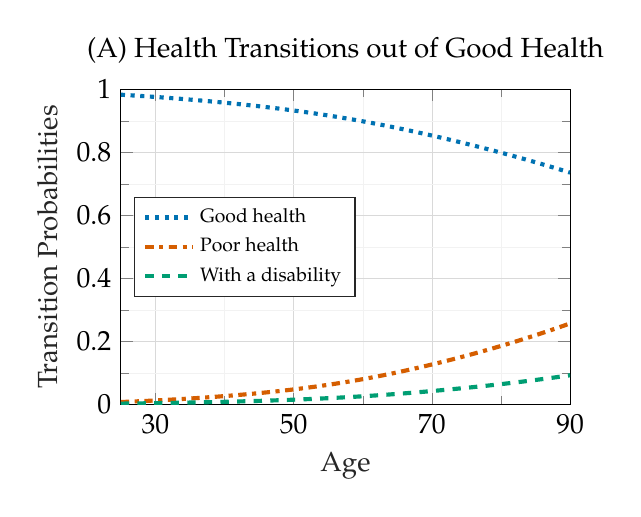
\begin{tikzpicture}
\begin{axis}[%
width=5.706cm,
height=4cm,
at={(0cm,0cm)},
scale only axis,
xmin=25,
xmax=90,
xtick={30,50,70,90},
xlabel style={font=\color{white!15!black}},
xlabel={Age},
ymin=0,
ymax=1,
ylabel style={font=\color{white!15!black}},
ylabel={Transition Probabilities},
axis background/.style={fill=white},
%title style={font=\bfseries},
title={(A) Health Transitions out of Good Health},
legend style={at={(0.03,0.5)}, anchor=west, legend cell align=left, align=left, draw=white!15!black,font=\scriptsize},
grid=both,
grid style={line width=0.2pt, draw=gray!30},
minor grid style={line width=0.1pt, draw=gray!10},
minor tick num=1
]
% Blue line - h(t)=0 - dotted line
\addplot [color=blue, line width=1.5pt, dotted]
  table[row sep=crcr]{%
25 0.98309247\\
26 0.98177065\\
27 0.98040043\\
28 0.97898087\\
29 0.97751107\\
30 0.97599011\\
31 0.97441706\\
32 0.97279099\\
33 0.97111097\\
34 0.96937609\\
35 0.96758542\\
36 0.96573805\\
37 0.96383308\\
38 0.96186959\\
39 0.95984659\\
40 0.95776298\\
41 0.95561743\\
42 0.95340817\\
43 0.95113281\\
44 0.94878801\\
45 0.94636924\\
46 0.94387079\\
47 0.94128627\\
48 0.93861018\\
49 0.93583981\\
50 0.93297328\\
51 0.93000876\\
52 0.92694444\\
53 0.92377856\\
54 0.92050939\\
55 0.91713528\\
56 0.91365461\\
57 0.91006583\\
58 0.90636744\\
59 0.90255801\\
60 0.89863619\\
61 0.89460071\\
62 0.89045035\\
63 0.88618399\\
64 0.88180192\\
65 0.87730914\\
66 0.87271271\\
67 0.86801917\\
68 0.86323358\\
69 0.85835934\\
70 0.85339844\\
71 0.84835184\\
72 0.8432198\\
73 0.83800218\\
74 0.83269856\\
75 0.82730842\\
76 0.82183118\\
77 0.81626625\\
78 0.81061306\\
79 0.80487101\\
80 0.79903956\\
81 0.79311816\\
82 0.78710628\\
83 0.78100339\\
84 0.77480897\\
85 0.76852255\\
86 0.76214369\\
87 0.75567204\\
88 0.74910741\\
89 0.74244985\\
90 0.73569986\\
};
\addlegendentry{Good health}

% Red line - h(t)=1 - dash-dotted line
\addplot [color=red, line width=1.5pt, dashdotted]
  table[row sep=crcr]{%
25 0.00740989\\
26 0.00829385\\
27 0.0092242\\
28 0.01020239\\
29 0.01122993\\
30 0.01230832\\
31 0.01343908\\
32 0.01462377\\
33 0.01586393\\
34 0.01716114\\
35 0.01851696\\
36 0.01993295\\
37 0.02141069\\
38 0.02295175\\
39 0.02455777\\
40 0.02623054\\
41 0.02797205\\
42 0.02978474\\
43 0.03167175\\
44 0.0336372\\
45 0.03568655\\
46 0.03782661\\
47 0.04006511\\
48 0.04240901\\
49 0.04486246\\
50 0.04742877\\
51 0.05011122\\
52 0.05291311\\
53 0.05583768\\
54 0.05888815\\
55 0.0620677\\
56 0.06537945\\
57 0.06882647\\
58 0.07241176\\
59 0.07613823\\
60 0.08000872\\
61 0.08402595\\
62 0.08819256\\
63 0.09251107\\
64 0.09698204\\
65 0.10159943\\
66 0.10635428\\
67 0.1112381\\
68 0.11624445\\
69 0.12136908\\
70 0.1266097\\
71 0.13196542\\
72 0.13743634\\
73 0.14302316\\
74 0.14872693\\
75 0.15454888\\
76 0.16049033\\
77 0.16655263\\
78 0.1727371\\
79 0.17904508\\
80 0.18547785\\
81 0.1920367\\
82 0.19872287\\
83 0.20553761\\
84 0.21248211\\
85 0.21955753\\
86 0.22676493\\
87 0.23410525\\
88 0.24157916\\
89 0.24918697\\
90 0.25692832\\
};
\addlegendentry{Poor health}

% Green line - h(t)=2 - dashed line
\addplot [color=green, line width=1.5pt, dashed]
  table[row sep=crcr]{%
25 0.00232342\\
26 0.00258882\\
27 0.00286849\\
28 0.00316296\\
29 0.00347276\\
30 0.00379847\\
31 0.00414063\\
32 0.00449986\\
33 0.00487673\\
34 0.00527188\\
35 0.00568592\\
36 0.00611948\\
37 0.00657321\\
38 0.00704778\\
39 0.00754387\\
40 0.00806223\\
41 0.0086037\\
42 0.00916924\\
43 0.00976009\\
44 0.0103778\\
45 0.01102439\\
46 0.01170237\\
47 0.0124146\\
48 0.01316373\\
49 0.01395159\\
50 0.01477974\\
51 0.0156498\\
52 0.01656341\\
53 0.01752226\\
54 0.01852807\\
55 0.01958259\\
56 0.02068762\\
57 0.02184496\\
58 0.02305648\\
59 0.02432406\\
60 0.02564961\\
61 0.02703505\\
62 0.02848236\\
63 0.02999351\\
64 0.03156963\\
65 0.03320868\\
66 0.03490704\\
67 0.03666119\\
68 0.03846841\\
69 0.040327\\
70 0.04223612\\
71 0.04419564\\
72 0.04620591\\
73 0.04826763\\
74 0.05038168\\
75 0.05254912\\
76 0.05477106\\
77 0.0570487\\
78 0.05938328\\
79 0.06177607\\
80 0.0642284\\
81 0.06674166\\
82 0.06931726\\
83 0.07195667\\
84 0.07466143\\
85 0.07743309\\
86 0.08027324\\
87 0.08318347\\
88 0.08616529\\
89 0.08922008\\
90 0.0923489\\
};
\addlegendentry{With a disability}
\end{axis}
\end{tikzpicture} & 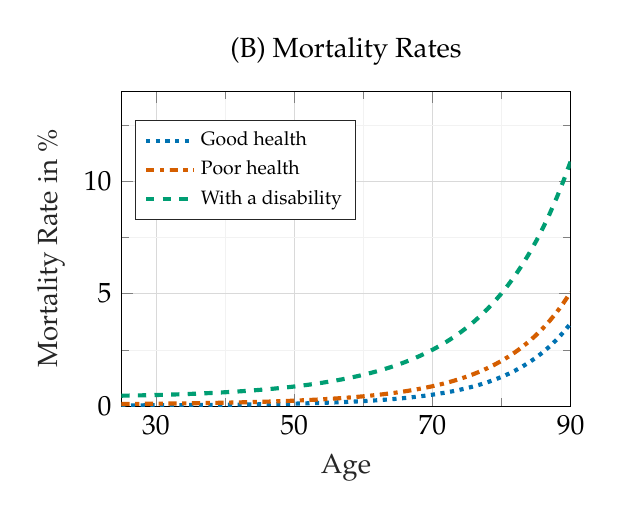
\begin{tikzpicture}
\begin{axis}[%
width=5.706cm,
height=4cm,
at={(0cm,0cm)},
scale only axis,
xmin=25,
xmax=90,
xtick={30,50,70,90},
xlabel style={font=\color{white!15!black}},
xlabel={Age},
ymin=0,
ymax=14,
ylabel style={font=\color{white!15!black}},
ylabel={Mortality Rate in \%},
axis background/.style={fill=white},
%title style={font=\bfseries},
title={(B) Mortality Rates},
legend style={at={(axis cs:27,10.5)}, anchor=west, legend cell align=left, align=left, draw=white!15!black, font=\scriptsize},
grid=both,
grid style={line width=0.2pt, draw=gray!30},
minor grid style={line width=0.1pt, draw=gray!10},
minor tick num=1
]
% Back line (Overall) - full
% \addplot [color=black, line width=1.5pt]
%   table[row sep=crcr]{%
% 25 0.04479\\
% 26 0.04675\\
% 27 0.0481\\
% 28 0.05082\\
% 29 0.05277\\
% 30 0.05375\\
% 31 0.05639\\
% 32 0.05905\\
% 33 0.06249\\
% 34 0.06579\\
% 35 0.06926\\
% 36 0.07637\\
% 37 0.07822\\
% 38 0.08325\\
% 39 0.08796\\
% 40 0.09379\\
% 41 0.09919\\
% 42 0.10925\\
% 43 0.11504\\
% 44 0.12074\\
% 45 0.12909\\
% 46 0.13868\\
% 47 0.1475\\
% 48 0.15626\\
% 49 0.16962\\
% 50 0.18554\\
% 51 0.20082\\
% 52 0.21588\\
% 53 0.23697\\
% 54 0.25106\\
% 55 0.27595\\
% 56 0.30314\\
% 57 0.32832\\
% 58 0.35589\\
% 59 0.38782\\
% 60 0.41329\\
% 61 0.45229\\
% 62 0.48501\\
% 63 0.52826\\
% 64 0.55276\\
% 65 0.59562\\
% 66 0.66072\\
% 67 0.70075\\
% 68 0.74535\\
% 69 0.80985\\
% 70 0.87603\\
% 71 1.00144\\
% 72 1.03708\\
% 73 1.21095\\
% 74 1.28609\\
% 75 1.47924\\
% 76 1.53636\\
% 77 1.74536\\
% 78 1.86332\\
% 79 2.00865\\
% 80 2.31624\\
% 81 2.51996\\
% 82 2.79552\\
% 83 3.17659\\
% 84 3.35743\\
% 85 3.97544\\
% 86 4.09512\\
% 87 4.87983\\
% 88 5.39166\\
% 89 6.00628\\
% 90 6.48326\\
% };
% \addlegendentry{Overall}
% Blue line (Good health) - dotted
\addplot [color=blue, line width=1.5pt, dotted]
  table[row sep=crcr]{%
25 0.035\\
26 0.03614\\
27 0.03736\\
28 0.03868\\
29 0.04009\\
30 0.0416\\
31 0.04323\\
32 0.04497\\
33 0.04685\\
34 0.04886\\
35 0.05103\\
36 0.05335\\
37 0.05586\\
38 0.05855\\
39 0.06146\\
40 0.06458\\
41 0.06795\\
42 0.07159\\
43 0.07552\\
44 0.07975\\
45 0.08434\\
46 0.0893\\
47 0.09467\\
48 0.10049\\
49 0.1068\\
50 0.11365\\
51 0.12109\\
52 0.12917\\
53 0.13798\\
54 0.14756\\
55 0.158\\
56 0.1694\\
57 0.18184\\
58 0.19545\\
59 0.21032\\
60 0.22662\\
61 0.24448\\
62 0.26407\\
63 0.28558\\
64 0.30923\\
65 0.33525\\
66 0.3639\\
67 0.39548\\
68 0.43033\\
69 0.46882\\
70 0.51137\\
71 0.55844\\
72 0.61059\\
73 0.66839\\
74 0.73254\\
75 0.80378\\
76 0.88297\\
77 0.97108\\
78 1.06919\\
79 1.17854\\
80 1.3005\\
81 1.43664\\
82 1.58871\\
83 1.75871\\
84 1.94885\\
85 2.16166\\
86 2.39997\\
87 2.66694\\
88 2.96613\\
89 3.30152\\
90 3.67755\\
};
\addlegendentry{Good health}

% Red line (Poor health) - dash-dotted
\addplot [color=red, line width=1.5pt, dashdotted]
  table[row sep=crcr]{%
25 0.09962\\
26 0.10175\\
27 0.10405\\
28 0.10654\\
29 0.10922\\
30 0.11212\\
31 0.11523\\
32 0.11858\\
33 0.12218\\
34 0.12605\\
35 0.1302\\
36 0.13466\\
37 0.13944\\
38 0.14458\\
39 0.15009\\
40 0.15601\\
41 0.16236\\
42 0.16919\\
43 0.17652\\
44 0.18441\\
45 0.19288\\
46 0.202\\
47 0.21181\\
48 0.22237\\
49 0.23376\\
50 0.24603\\
51 0.25927\\
52 0.27356\\
53 0.289\\
54 0.30569\\
55 0.32375\\
56 0.3433\\
57 0.36448\\
58 0.38745\\
59 0.41237\\
60 0.43943\\
61 0.46884\\
62 0.50084\\
63 0.53568\\
64 0.57364\\
65 0.61503\\
66 0.66022\\
67 0.70958\\
68 0.76354\\
69 0.82259\\
70 0.88726\\
71 0.95816\\
72 1.03592\\
73 1.12131\\
74 1.21513\\
75 1.31831\\
76 1.43187\\
77 1.55694\\
78 1.6948\\
79 1.84687\\
80 2.01472\\
81 2.20011\\
82 2.40499\\
83 2.63155\\
84 2.8822\\
85 3.15962\\
86 3.46679\\
87 3.80701\\
88 4.1839\\
89 4.60146\\
90 5.06408\\
};
\addlegendentry{Poor health}

% Green line (With a Disability) - dashed
\addplot [color=green, line width=1.5pt, dashed]
  table[row sep=crcr]{%
25 0.46695\\
26 0.47172\\
27 0.47714\\
28 0.48322\\
29 0.48999\\
30 0.49748\\
31 0.50572\\
32 0.51473\\
33 0.52456\\
34 0.53524\\
35 0.54682\\
36 0.55934\\
37 0.57287\\
38 0.58745\\
39 0.60316\\
40 0.62006\\
41 0.63821\\
42 0.65772\\
43 0.67867\\
44 0.70115\\
45 0.72527\\
46 0.75115\\
47 0.77892\\
48 0.8087\\
49 0.84066\\
50 0.87496\\
51 0.91177\\
52 0.9513\\
53 0.99376\\
54 1.03937\\
55 1.0884\\
56 1.14113\\
57 1.19786\\
58 1.25892\\
59 1.32469\\
60 1.39555\\
61 1.47196\\
62 1.55439\\
63 1.64337\\
64 1.73947\\
65 1.84333\\
66 1.95565\\
67 2.07718\\
68 2.20877\\
69 2.35133\\
70 2.50586\\
71 2.67347\\
72 2.85536\\
73 3.05287\\
74 3.26744\\
75 3.50067\\
76 3.75428\\
77 4.03018\\
78 4.33044\\
79 4.65732\\
80 5.01328\\
81 5.40098\\
82 5.82331\\
83 6.28341\\
84 6.78464\\
85 7.33061\\
86 7.92519\\
87 8.57248\\
88 9.27686\\
89 10.04289\\
90 10.87536\\
};
\addlegendentry{With a disability}
\end{axis}
\end{tikzpicture} \\[1ex]
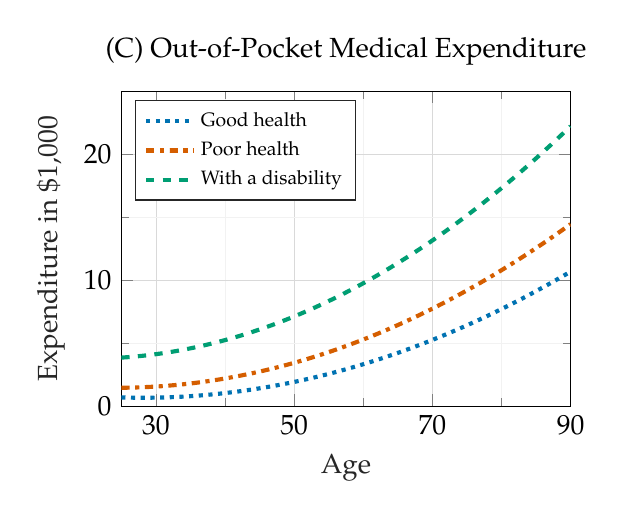
\begin{tikzpicture}
\begin{axis}[%
width=5.706cm,
height=4cm,
at={(0cm,0cm)},
scale only axis,
xmin=25,
xmax=90,
xtick={30,50,70,90},
xlabel style={font=\color{white!15!black}},
xlabel={Age},
ymin=0,
ymax=25,
ylabel style={font=\color{white!15!black}},
ylabel={Expenditure in \$1,000},
axis background/.style={fill=white},
%title style={font=\bfseries},
title={(C) Out-of-Pocket Medical Expenditure},
legend style={at={(axis cs:27,20.3)}, anchor=west, legend cell align=left, align=left, draw=white!15!black, font=\scriptsize},
grid=both,
grid style={line width=0.2pt, draw=gray!30},
minor grid style={line width=0.1pt, draw=gray!10},
minor tick num=1
]
% Blue line (h(t)=0) - dotted
\addplot [color=blue, line width=1.5pt, dotted]
  table[row sep=crcr]{%
25 0.69549069\\
26 0.68199083\\
27 0.67371464\\
28 0.6706623\\
29 0.67283363\\
30 0.68022881\\
31 0.69284784\\
32 0.71069035\\
33 0.73375671\\
34 0.76204674\\
35 0.79556062\\
36 0.83429816\\
37 0.87825956\\
38 0.92744462\\
39 0.98185335\\
40 1.04148593\\
41 1.10634236\\
42 1.17642228\\
43 1.25172585\\
44 1.33225347\\
45 1.41800457\\
46 1.5089797\\
47 1.60517831\\
48 1.70660078\\
49 1.81324709\\
50 1.92511801\\
51 2.04221129\\
52 2.16452841\\
53 2.29206939\\
54 2.42483423\\
55 2.56282291\\
56 2.70603545\\
57 2.85447183\\
58 3.00813021\\
59 3.1670143\\
60 3.33112225\\
61 3.50045404\\
62 3.67500783\\
63 3.85478546\\
64 4.03978882\\
65 4.23001602\\
66 4.42546521\\
67 4.62613826\\
68 4.83203516\\
69 5.0431559\\
70 5.25950051\\
71 5.48107082\\
72 5.70786313\\
73 5.93987742\\
74 6.17711743\\
75 6.41958129\\
76 6.667269\\
77 6.92017871\\
78 7.17831412\\
79 7.44167339\\
80 7.71025465\\
81 7.98406162\\
82 8.26309058\\
83 8.5473434\\
84 8.83682006\\
85 9.13152245\\
86 9.43144682\\
87 9.73659504\\
88 10.0469652\\
89 10.362563\\
90 10.6833828\\
};
\addlegendentry{Good health}

% Red line (h(t)=1) - dash-dotted
\addplot [color=red, line width=1.5pt, dashdotted]
  table[row sep=crcr]{%
25 1.46408419\\
26 1.47088973\\
27 1.48372673\\
28 1.50259464\\
29 1.52749401\\
30 1.55842446\\
31 1.59538601\\
32 1.63837884\\
33 1.68740294\\
34 1.74245794\\
35 1.8035444\\
36 1.87066252\\
37 1.94381135\\
38 2.02299071\\
39 2.10820247\\
40 2.19944476\\
41 2.29671758\\
42 2.40002279\\
43 2.50935854\\
44 2.62472481\\
45 2.74612348\\
46 2.87355268\\
47 3.00701427\\
48 3.14650454\\
49 3.29202905\\
50 3.44358224\\
51 3.60116782\\
52 3.76478393\\
53 3.93443244\\
54 4.11011148\\
55 4.29182105\\
56 4.47956301\\
57 4.6733355\\
58 4.87313852\\
59 5.07897394\\
60 5.29083989\\
61 5.50873637\\
62 5.73266525\\
63 5.96262465\\
64 6.19861645\\
65 6.44063878\\
66 6.68869164\\
67 6.94277503\\
68 7.20289082\\
69 7.46903714\\
70 7.74121585\\
71 8.01942509\\
72 8.30366486\\
73 8.59393703\\
74 8.89023973\\
75 9.19257296\\
76 9.50093858\\
77 9.81533473\\
78 10.1357614\\
79 10.4622205\\
80 10.7947101\\
81 11.1332302\\
82 11.4777846\\
83 11.8283658\\
84 12.1849813\\
85 12.5476292\\
86 12.9163038\\
87 13.2910127\\
88 13.6717522\\
89 14.0585203\\
90 14.4513245\\
};
\addlegendentry{Poor health}

% Green line (h(t)=2) - dashed
\addplot [color=green, line width=1.5pt, dashed]
  table[row sep=crcr]{%
25 3.85542075\\
26 3.89487722\\
27 3.94193474\\
28 3.99658957\\
29 4.05884358\\
30 4.12869677\\
31 4.20614726\\
32 4.29119694\\
33 4.38384579\\
34 4.48409196\\
35 4.5919373\\
36 4.70738183\\
37 4.83042552\\
38 4.9610684\\
39 5.09930859\\
40 5.24514795\\
41 5.3985865\\
42 5.55962235\\
43 5.72825925\\
44 5.90449346\\
45 6.08832499\\
46 6.27975755\\
47 6.47878743\\
48 6.68541649\\
49 6.89964472\\
50 7.12147213\\
51 7.35089685\\
52 7.58792075\\
53 7.83254383\\
54 8.08476422\\
55 8.34458379\\
56 8.61200254\\
57 8.88702046\\
58 9.16963756\\
59 9.45985011\\
60 9.7576637\\
61 10.0630765\\
62 10.3760884\\
63 10.6966977\\
64 11.0249061\\
65 11.3607119\\
66 11.7041168\\
67 12.0551246\\
68 12.4137279\\
69 12.7799285\\
70 13.1537301\\
71 13.5351272\\
72 13.9241253\\
73 14.3207226\\
74 14.7249191\\
75 15.1367111\\
76 15.5561059\\
77 15.983098\\
78 16.4176856\\
79 16.8598761\\
80 17.3096621\\
81 17.7670491\\
82 18.2320353\\
83 18.7046132\\
84 19.1848014\\
85 19.6725907\\
86 20.1679624\\
87 20.6709351\\
88 21.1815089\\
89 21.6997024\\
90 22.2254782\\
};
\addlegendentry{With a disability}
\end{axis}
\end{tikzpicture} & 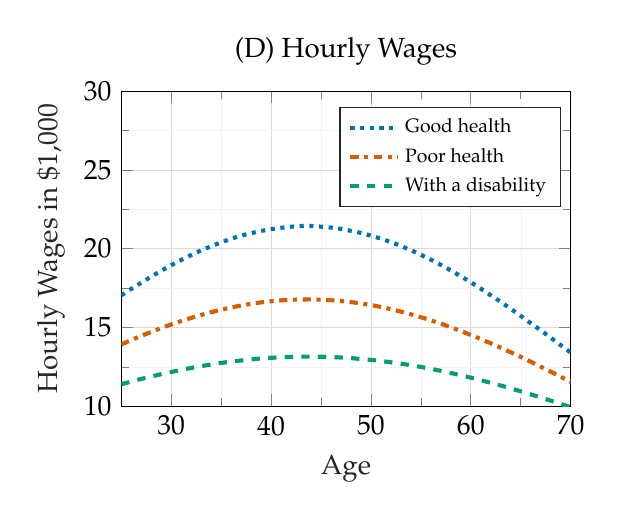
\begin{tikzpicture}
\begin{axis}[%
width=5.706cm,
height=4cm,
at={(0cm,0cm)},
scale only axis,
xmin=25,
xmax=70,
xlabel style={font=\color{white!15!black}},
xlabel={Age},
ymin=10,
ymax=30,
ylabel style={font=\color{white!15!black}},
ylabel={Hourly Wages in \$1,000},
axis background/.style={fill=white},
%title style={font=\bfseries},
title={(D) Hourly Wages},
legend style={at={(axis cs:69,29)}, anchor=north east, legend cell align=left, align=left, draw=white!15!black, font=\scriptsize},
grid=both,
grid style={line width=0.2pt, draw=gray!30},
minor grid style={line width=0.1pt, draw=gray!10},
minor tick num=1
]
% Blue line (h(t)=0) - dotted
\addplot [color=blue, line width=1.5pt, dotted]
  table[row sep=crcr]{%
25 17.038732931\\
26 17.4542862\\
27 17.8458896\\
28 18.2333825\\
29 18.6034326\\
30 18.9545214\\
31 19.2874174\\
32 19.6000282\\
33 19.8910738\\
34 20.1595058\\
35 20.4032752\\
36 20.6349778\\
37 20.8299873\\
38 20.9875306\\
39 21.1294096\\
40 21.2430726\\
41 21.3293168\\
42 21.3971419\\
43 21.4465891\\
44 21.4472714\\
45 21.4000386\\
46 21.3431199\\
47 21.2595208\\
48 21.1359871\\
49 21.0057627\\
50 20.8289922\\
51 20.6396637\\
52 20.4187952\\
53 20.1755905\\
54 19.9054845\\
55 19.6151301\\
56 19.3050955\\
57 18.9731394\\
58 18.6231478\\
59 18.2534162\\
60 17.8725251\\
61 17.4667029\\
62 17.0430688\\
63 16.6240313\\
64 16.1871244\\
65 15.7395087\\
66 15.2739585\\
67 14.8207176\\
68 14.3532838\\
69 13.8810528\\
70 13.4097773\\
71 12.9349057\\
72 12.4596877\\
73 11.9863954\\
74 11.5156889\\
75 11.0495625\\
76 10.5862582\\
77 10.1178357\\
78 9.6800105\\
79 9.2399334\\
80 8.8042616\\
81 8.3797474\\
82 7.9649453\\
83 7.5606193\\
84 7.1672203\\
85 6.7840423\\
86 6.4149422\\
87 6.0569024\\
88 5.7111602\\
89 5.3778823\\
90 5.0573577\\
};
\addlegendentry{Good health}

% Red line (h(t)=1) - dash-dotted
\addplot [color=red, line width=1.5pt, dashdotted]
  table[row sep=crcr]{%
25 13.9207948\\
26 14.2047403\\
27 14.4674653\\
28 14.7182134\\
29 14.9623434\\
30 15.1910459\\
31 15.4087123\\
32 15.6087075\\
33 15.7961556\\
34 15.9738525\\
35 16.1282511\\
36 16.2684047\\
37 16.3923221\\
38 16.5039362\\
39 16.5943431\\
40 16.6654026\\
41 16.7207774\\
42 16.7588626\\
43 16.7789271\\
44 16.7809953\\
45 16.7649334\\
46 16.7304199\\
47 16.6802994\\
48 16.6140951\\
49 16.5227746\\
50 16.4246175\\
51 16.3035138\\
52 16.1600103\\
53 16.0063856\\
54 15.8372274\\
55 15.6530267\\
56 15.4545121\\
57 15.2417903\\
58 15.0159812\\
59 14.7776676\\
60 14.5274988\\
61 14.2621611\\
62 13.9945643\\
63 13.7143475\\
64 13.4233456\\
65 13.1343654\\
66 12.8222313\\
67 12.5077179\\
68 12.1916875\\
69 11.8699484\\
70 11.5442478\\
71 11.2153607\\
72 10.8822157\\
73 10.5514423\\
74 10.2179713\\
75 9.8842727\\
76 9.5512479\\
77 9.2185561\\
78 8.8888729\\
79 8.5626167\\
80 8.2386738\\
81 7.9184131\\
82 7.6024837\\
83 7.2932698\\
84 6.9862644\\
85 6.6848614\\
86 6.3906564\\
87 6.0569024\\
88 5.7111602\\
89 5.3778823\\
90 5.0573577\\
};
\addlegendentry{Poor health}

% Green line (h(t)=2) - dashed
\addplot [color=green, line width=1.5pt, dashed]
  table[row sep=crcr]{%
25 11.3963276\\
26 11.5667395\\
27 11.7321955\\
28 11.8862335\\
29 12.0326526\\
30 12.1689006\\
31 12.3078104\\
32 12.4301344\\
33 12.5440848\\
34 12.6468777\\
35 12.7489912\\
36 12.8328886\\
37 12.9037903\\
38 12.9716965\\
39 13.0340029\\
40 13.0733775\\
41 13.1080689\\
42 13.1321171\\
43 13.1455988\\
44 13.1483318\\
45 13.1403785\\
46 13.1218273\\
47 13.0926326\\
48 13.0528585\\
49 13.0016644\\
50 12.9431201\\
51 12.8703837\\
52 12.7866147\\
53 12.7004345\\
54 12.6064182\\
55 12.4933071\\
56 12.3756657\\
57 12.2442144\\
58 12.1086155\\
59 11.9659139\\
60 11.8118108\\
61 11.6521229\\
62 11.4852695\\
63 11.3116547\\
64 11.1304946\\
65 10.9473952\\
66 10.7536501\\
67 10.5566969\\
68 10.354914\\
69 10.1486702\\
70 9.9385408\\
71 9.7247835\\
72 9.5079214\\
73 9.2853921\\
74 9.0644669\\
75 8.8426994\\
76 8.6174101\\
77 8.3910749\\
78 8.1640136\\
79 7.9366855\\
80 7.7074157\\
81 7.4825711\\
82 7.2584391\\
83 7.0344812\\
84 6.8119217\\
85 6.5861317\\
86 6.3664108\\
87 6.0569024\\
88 5.7111602\\
89 5.3778823\\
90 5.0573577\\
};
\addlegendentry{With a disability}
\end{axis}
\end{tikzpicture}
\end{tabular}
\tabnotes{\textit{Notes:} Panel A shows the probability of being in good health, in poor health, or with a disability at age $t+1$ for an individual in good health at age $t$. Panel B shows annual mortality rates (percent), panel C annual out-of-pocket medical expenditures (thousands of dollars), and panel D offered hourly wages corrected for selection (dollars), by age and health status. Blue dotted, red dash-dotted, and green dashed lines refer to good health, poor health, and disability. Monetary values are in 2016 dollars. \textit{Data sources:} Panel Study of Income Dynamics (panels A, B, and D) and Medical Expenditure Panel Survey (panel C).}
\end{figure}

\begin{table}[!htbp]
\centering
\caption{First-Step and Calibrated Parameters}\label{tab:calibrated}
\small
% Table body for tab:calibrated (Section 3).
% Sources: FROT tables/parameters_summary.tex (rho = 0.981, sigma^2 = 0.016, ERA 62, NRA 65, DRC 4.5%; scratchpad src/tables/parameters_summary.tex);
% r_f = 4%, 20% wedge, consumption floor $3,500: FROT 2025_sub/5_quantitative_model.tex (First-Step Estimation) and blueprint Sec. 5; floor attribution corrected to French2004.
\begin{tabular}{@{}l l l l@{}}
\toprule
Parameter & Description & Value & Source \\
\midrule
\multicolumn{4}{@{}l}{\textit{A. Estimated from data outside the model}} \\
$\pi_{j,i,t+1}$ & Health transition probabilities & Fig.~\ref{fig:firststep}A & PSID \\
$S(h,t)$ & Survival probabilities & Fig.~\ref{fig:firststep}B & PSID \\
$M(h,t,P)$ & Out-of-pocket medical expenses & Fig.~\ref{fig:firststep}C & MEPS \\
$W(h,t)$ & Deterministic wage profiles & Fig.~\ref{fig:firststep}D & PSID \\
$\rho$ & Autocorrelation of log ability & 0.981 & PSID \\
$\sigma^2$ & Variance of ability innovations & 0.016 & PSID \\
$\lambda_t,\tau_t$ & Income tax function by age & Age-specific & \citet{Borella2023} \\
\addlinespace
\multicolumn{4}{@{}l}{\textit{B. Taken from the literature}} \\
% AUTHORS: the r_f (French 2005) and tau_k (Stantcheva 2017) attributions follow FROT 2025_sub/5_quantitative_model.tex; a reviewer could not locate either value in the cited papers. Add page/table references or cite the original sources.
$r_f$ & Gross interest rate & 4\% & \citet{french2005effects} \\
$\tau_k$ & Wedge between gross and net return & 20\% & \citet{Stantcheva2017} \\
$\underline{c}$ & Consumption floor & \$3,500 & \citet{French2004} \\ % Attribution per verified_facts item 8: $3,500 is French and Jones (2004, CRR WP 2004-12), not French and Jones (2011).
\addlinespace
\multicolumn{4}{@{}l}{\textit{C. Program rules, cohorts born 1920--1940}} \\
ERA & Early retirement age & 62 & SSA \\
NRA & Normal retirement age & 65 & SSA \\
DRC & Delayed retirement credit & 4.5\% & SSA \\
 & Other Social Security rules & Table~\ref{tab:ssparams} & SSA \\
\bottomrule
\end{tabular}

\tabnotes{\textit{Notes:} Parameters fixed before the second-step estimation. Panel A lists objects estimated directly from the data (Appendix~\ref{app:firststep}); $\rho$ and $\sigma^2$ are the autocorrelation and innovation variance of log ability $\ln\theta_t$; the income tax function $T_t(y)=y-\lambda_t y^{1-\tau_t}$ is estimated by age following \citet{Borella2023}. Panel B lists values taken from earlier studies; the net return on savings is $r=(1-\tau_k)r_f=3.2\%$. Panel C lists Social Security rules for the 1920--1940 birth cohorts; the DRC is the cohort average of credits that varied with the year of birth. Abbreviations: ERA, early retirement age; NRA, normal retirement age; DRC, delayed retirement credit; PSID, Panel Study of Income Dynamics; MEPS, Medical Expenditure Panel Survey; SSA, Social Security Administration.}
\end{table}

\subsection{Second-Step Estimation by the Method of Simulated Moments}

\paragraph{Moments and criterion.} For each age from 30 to 69 ($T=40$ ages), we match seven moments: the participation rates of healthy and unhealthy individuals, the mean annual hours of healthy and unhealthy participants, mean and median nonpension assets, and the mean reentry rate. This yields $7\times 40=280$ moment conditions. Because the labor-supply moments pool poor health and disability, the two states share a fixed cost of participation, $\phi_n(1)=\phi_n(2)$.

Let $\hat{\varphi}(\mathcal{P};\chi)$ denote the 280-element vector of differences between the data moments and the corresponding moments of the model, simulated from the decision rules (Appendix~\ref{app:solution}) for individuals who start from the empirical distribution of initial conditions and draw health, survival, and wage shocks from the first-step processes. The MSM estimator is
\[
\hat{\mathcal{P}}=\argmin_{\mathcal{P}}\ \frac{N}{1+N/N_s}\ \hat{\varphi}(\mathcal{P};\chi)'\,\hat{\mathbf{W}}\,\hat{\varphi}(\mathcal{P};\chi),
\]
where $N$ is the number of observations in the data, $N_s$ is the number of simulated observations, and the factor $1+N/N_s$ accounts for simulation error. The weighting matrix $\hat{\mathbf{W}}$ is the inverse of a diagonal matrix that holds the sampling variances of the data moments, so each moment is weighted by its precision. Appendix~\ref{app:msm} lists the moment conditions and the estimation algorithm and derives the standard errors.

\paragraph{Identification.} As in \citet{french2005effects}, identification rests on two assumptions: work decisions do not affect health or wages, and age shifts the incentives to work and save---through wages, health, mortality, medical expenses, and the rules of Social Security and pensions---but not preferences. Under these assumptions, the first step measures how incentives change with age and health, and the behavior that these incentives do not explain identifies preferences. The discount factor $\beta$ is identified by intertemporal substitution, and hence by the asset and labor-supply profiles, especially at the ages at which individuals accumulate wealth for retirement. The time endowment $L$ and the fixed costs $\phi_n(h)$ are identified by participation and hours by health status: with a fixed cost, individuals either work substantial hours or do not work at all, so the participation rate and the hours of those who work carry separate information, and the gap between the participation profiles of healthy and unhealthy individuals, given their first-step wages and medical costs, pins down the health gradient in the fixed cost. The reentry cost $\phi_{RE}$ is identified by the low reentry rates in the data. The curvature parameters $\nu$ and $\gamma$ are identified by the asset and labor-supply profiles: higher risk aversion raises precautionary saving and encourages more work earlier in life.

\subsection{Parameter Estimates}

\autoref{tab:estimates} reports the estimates. The discount factor is 0.98. The annual time endowment is 4,491 hours, and the fixed cost of working is 791 hours for healthy individuals and 868 hours for individuals in poor health or with a disability. A healthy participant thus gives up about 18 percent of her time endowment before working the first hour, and an unhealthy participant about 19 percent (ratios of the table entries, $791.07/4490.5$ and $867.54/4490.5$). This nonconvexity is what makes retirement a discrete decision in the model: workers choose between substantial hours and full exit, so a reform moves labor supply mainly by changing the age of exit. The health gradient in the fixed cost compounds the lower wages, higher medical expenses, and access to DI of unhealthy individuals, each of which also pulls their exit forward. The time endowment and the fixed costs fall within the range of estimates in \citet{french2011effects} and \citet{Borella2023}.

The reentry cost is 3,312 hours, about three-quarters of the annual time endowment (the ratio $3311.5/4490.5$). Leaving the labor force is therefore close to irreversible, and a reform that encourages later retirement acts on workers before they exit rather than drawing retirees back into work.

The curvature of flow utility is $\nu=1.70$ and the consumption weight is $\gamma=0.54$, which imply a coefficient of relative risk aversion over consumption, $-u_{cc}c/u_c=1-\gamma(1-\nu)$, of approximately 1.38. Because $\nu>1$, the marginal utility of consumption falls as leisure rises, so consumption optimally declines at retirement. The two parameters also scale the consumption-equivalent welfare measure of Section~\ref{sec:fw_welfare}, which converts changes in expected utility into changes in consumption through $\gamma(1-\nu)$.

The overidentification statistic is 1463 with $280-7=273$ degrees of freedom, so the test formally rejects the model, as in earlier studies that estimate life-cycle retirement models on many precisely measured moments \citep{french2005effects,french2011effects}. The test asks the model to match 280 profiles at every age within sampling error; the relevant question for our purposes is whether it reproduces the patterns of labor supply and saving through which retirement reforms operate, to which we now turn.

\begin{table}[!htbp]
\centering
\caption{Estimated Preference Parameters}\label{tab:estimates}
\small
% Table body for tab:estimates (Section 3).
% Source: FROT tables/estimated_parameters.tex (scratchpad copy: src/tables/estimated_parameters.tex).
% Every estimate, standard error, and the chi-square statistic is copied exactly; rows regrouped only.
\begin{tabular}{@{}l l r r@{}}
\toprule
Parameter & Description & Estimate & Std.\ error \\
\midrule
\multicolumn{4}{@{}l}{\textit{Preferences}} \\
$\gamma$ & Consumption weight & 0.5354 & 0.0047 \\
$\nu$ & Curvature of the consumption--leisure composite & 1.7029 & 0.0681 \\
$\beta$ & Time discount factor & 0.9797 & 0.0023 \\
\addlinespace
\multicolumn{4}{@{}l}{\textit{Time endowment and time costs (hours per year)}} \\
$L$ & Time endowment & 4490.5 & 21.65 \\
$\phi_n(0)$ & Fixed cost of work, good health & 791.07 & 15.65 \\
$\phi_n(1)=\phi_n(2)$ & Fixed cost of work, poor health or disability & 867.54 & 22.68 \\
$\phi_{RE}$ & Labor market reentry cost & 3311.5 & 82.02 \\
\midrule
\multicolumn{2}{@{}l}{Overidentification statistic, $\chi^2$ (273 degrees of freedom)} & 1463 & \\
\bottomrule
\end{tabular}

\tabnotes{\textit{Notes:} Method-of-simulated-moments estimates of the preference parameters and their asymptotic standard errors (Appendix~\ref{app:msm}). $\gamma$ is the weight on consumption and $\nu$ the curvature in $u(c,l)=(c^{\gamma}l^{1-\gamma})^{1-\nu}/(1-\nu)$; the implied relative risk aversion over consumption is $1-\gamma(1-\nu)\approx1.38$. $L$, $\phi_n(h)$, and $\phi_{RE}$ are measured in hours per year; poor health ($h=1$) and disability ($h=2$) share one fixed cost of work. The overidentification statistic tests the 280 moment conditions against 7 parameters. \textit{Data source:} Panel Study of Income Dynamics.}
\end{table}

\subsection{Match of Moments}

\autoref{fig:fit_labor} compares the simulated profiles of participation and hours with their PSID counterparts and 95 percent confidence intervals. In the data, participation is high and stable in the 30s and 40s, declines from the early 50s for individuals in poor health or with a disability, and drops sharply in the 60s in both health groups. These declines coincide with falling wages and with growing retirement incentives from pensions and Social Security. The model reproduces these patterns. As emphasized by \citet{Yu2024}, the explicit disability state and DI benefits are essential for the decline in the participation of unhealthy individuals from their 50s: DI provides an alternative pathway out of the labor force for people with a disability \citep{Maestas2013,French2014,Low2015,Li2018}, and modeling it yields a closer fit for this group than in earlier work such as \citet{french2005effects}.

The departures are informative about where the model is weakest. For unhealthy individuals, the model overstates participation in the 40s and concentrates the decline at age 50, the age from which DI is available in the model, whereas the decline in the data is spread over the late 40s and early 50s. Between the late 50s and the mid-60s, simulated participation of the unhealthy lies at or below the lower bound of the confidence band, and simulated participation of the healthy lies slightly below the data around age 60: simulated exit is somewhat early. Hours of participants decline in the 60s in the model as in the data, but the model places the hours of unhealthy workers, and to a lesser extent those of healthy workers, below the data before age 60.

The fit of unhealthy participation between 55 and 69 matters for the reform analysis because these are the ages at which three exit routes compete for the same individuals: DI, which pays the primary insurance amount without an early-claiming reduction until the NRA; early claiming of reduced retirement benefits from age 62; and continued work. Claiming-age reforms shift the relative value of these routes. Raising the NRA lowers retirement benefits at every claiming age while extending the ages at which DI is paid; raising the DRC increases the reward for delay, which individuals with higher mortality value less. The resulting reallocation across programs is what the indirect fiscal effects of Section~\ref{sec:framework} measure. Because simulated exit of the unhealthy is somewhat early, the model, if anything, places fewer unhealthy workers at the margin between work and claiming at ages 62 to 64 than the data do.

\begin{figure}[!htbp]
\centering
\caption{Data and Simulated Profiles: Participation and Hours}\label{fig:fit_labor}
\vspace{0.5em}
% Fit panels: corrected 2026 re-simulation of the estimated model at the same estimates (FROT figures/abdou/*_c.tex), copied verbatim.
\begin{tabular}{@{}c@{\hspace{1.5em}}c@{}}
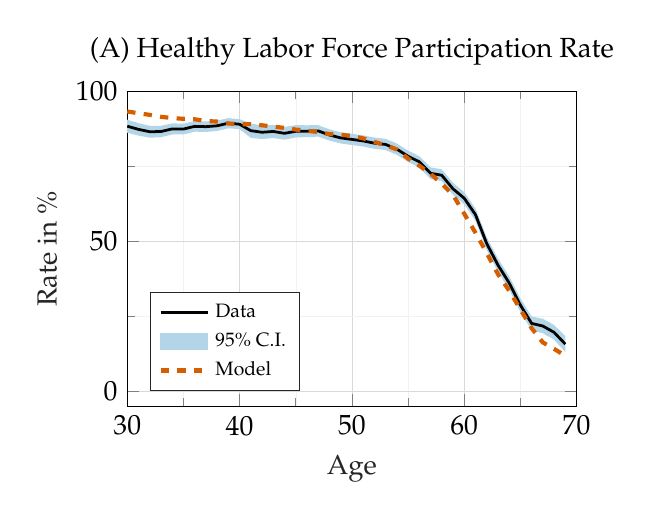
\begin{tikzpicture}
\begin{axis}[%
width=5.706cm,
height=4cm,
at={(0cm,0cm)},
scale only axis,
xmin=30,
xmax=70,
xlabel style={font=\color{white!15!black}},
xlabel={Age},
ymin=-5,
ymax=100,
ylabel style={font=\color{white!15!black}},
ylabel={Rate in \%},
axis background/.style={fill=white},
%title style={font=\bfseries},
title={(A) Healthy Labor Force Participation Rate},
legend style={at={(axis cs:32,0)}, anchor=south west, legend cell align=left, align=left, draw=white!15!black, font=\scriptsize},
grid=both,
grid style={line width=0.2pt, draw=gray!30},
minor grid style={line width=0.1pt, draw=gray!10},
minor tick num=1
]

% Main line (lfprlr0) - blue solid line
\addplot [color=black, line width=1pt]
  table[row sep=crcr, y expr=\thisrowno{1}*100]{%
30 0.8833822\\
31 0.8728638\\
32 0.8650124\\
33 0.8656822\\
34 0.8743696\\
35 0.873809\\
36 0.8829339\\
37 0.8818902\\
38 0.8847443\\
39 0.8934818\\
40 0.8900082\\
41 0.8684802\\
42 0.8632262\\
43 0.8659114\\
44 0.8597141\\
45 0.8664337\\
46 0.866869\\
47 0.8677746\\
48 0.8541223\\
49 0.8445035\\
50 0.8394285\\
51 0.8343548\\
52 0.8268231\\
53 0.8226036\\
54 0.8069361\\
55 0.7833442\\
56 0.7647346\\
57 0.7266455\\
58 0.7198906\\
59 0.6746376\\
60 0.6433743\\
61 0.5887213\\
62 0.4924323\\
63 0.4207888\\
64 0.3610537\\
65 0.2870897\\
66 0.2260264\\
67 0.21724\\
68 0.1962348\\
69 0.1569484\\
% 70 0.1681354\\
% 71 0.121358\\
% 72 0.1394618\\
% 73 0.1092736\\
% 74 0.1141775\\
% 75 0.0792269\\
% 76 0.0917666\\
% 77 0.0850947\\
% 78 0.0388536\\
% 79 0.0336195\\
% 80 0.058109\\
% 81 0.016314\\
% 82 0.0270162\\
% 83 -0.0089496\\
% 84 0.0236253\\
% 85 -0.0178846\\
};
\addlegendentry{Data}

% Upper bound (standard error high)
\addplot[name path=upper, draw=none, forget plot] 
  table[row sep=crcr,y expr=\thisrowno{1}*100]{%
30 0.9051051\\
31 0.8935855\\
32 0.8848711\\
33 0.88477\\
34 0.892873\\
35 0.8917789\\
36 0.9007229\\
37 0.8994025\\
38 0.9019169\\
39 0.9103903\\
40 0.9066504\\
41 0.8923349\\
42 0.8859496\\
43 0.8876875\\
44 0.8808528\\
45 0.8869151\\
46 0.88653\\
47 0.8869081\\
48 0.8729149\\
49 0.863117\\
50 0.858066\\
51 0.8529794\\
52 0.8455561\\
53 0.8413141\\
54 0.8257702\\
55 0.8021987\\
56 0.7835673\\
57 0.7460628\\
58 0.739598\\
59 0.6947576\\
60 0.663489\\
61 0.6094228\\
62 0.5136542\\
63 0.4426488\\
64 0.3833388\\
65 0.3098885\\
66 0.2493425\\
67 0.2413235\\
68 0.2207975\\
69 0.1832494\\
% 70 0.194256\\
% 71 0.1491448\\
% 72 0.1675596\\
% 73 0.1396055\\
% 74 0.1450964\\
% 75 0.1120739\\
% 76 0.1273876\\
% 77 0.1228318\\
% 78 0.0783176\\
% 79 0.0761687\\
% 80 0.1034711\\
% 81 0.0718914\\
% 82 0.080405\\
% 83 0.0504064\\
% 84 0.082339\\
% 85 0.0525297\\
};

% Lower bound (standard error low)
\addplot[name path=lower, draw=none, forget plot] 
  table[row sep=crcr,y expr=\thisrowno{1}*100]{%
30 0.8616592\\
31 0.852142\\
32 0.8451536\\
33 0.8465945\\
34 0.8558661\\
35 0.855839\\
36 0.8651446\\
37 0.8643779\\
38 0.8675715\\
39 0.8765733\\
40 0.8733659\\
41 0.8446254\\
42 0.8405027\\
43 0.8441353\\
44 0.8385755\\
45 0.8459523\\
46 0.8472079\\
47 0.848641\\
48 0.8353298\\
49 0.8258898\\
50 0.8207909\\
51 0.81573\\
52 0.80809\\
53 0.8038934\\
54 0.788102\\
55 0.7644898\\
56 0.7459021\\
57 0.7072282\\
58 0.7001832\\
59 0.6545175\\
60 0.6232595\\
61 0.5680198\\
62 0.4712104\\
63 0.3989288\\
64 0.3387687\\
65 0.2642909\\
66 0.2027102\\
67 0.1931565\\
68 0.1716722\\
69 0.1306474\\
% 70 0.1420148\\
% 71 0.0935712\\
% 72 0.111364\\
% 73 0.0789419\\
% 74 0.0832585\\
% 75 0.04638\\
% 76 0.0561455\\
% 77 0.0473576\\
% 78 -0.0006104\\
% 79 -0.0089297\\
% 80 0.012747\\
% 81 -0.0392634\\
% 82 -0.0263728\\
% 83 -0.0683057\\
% 84 -0.0350885\\
% 85 -0.0882989\\
};

% Fill between the paths
\addplot[blue!30] fill between[of=upper and lower];
\addlegendentry{95\% C.I.}

\addplot [color=red, line width=1.5pt, dashed]
  table[row sep=crcr,y expr=\thisrowno{1}*100]{%
30	0.932489451	\\
31	0.926638605	\\
32	0.921274038	\\
33	0.914777879	\\
34	0.910546993	\\
35	0.908122908	\\
36	0.906507791	\\
37	0.900768049	\\
38	0.898980538	\\
39	0.892446379	\\
40	0.889968652	\\
41	0.890397979	\\
42	0.886493342	\\
43	0.882240611	\\
44	0.877681716	\\
45	0.872236671	\\
46	0.868164063	\\
47	0.864026403	\\
48	0.85709527	\\
49	0.855082187	\\
50	0.850991114	\\
51	0.842930153	\\
52	0.831024931	\\
53	0.820189274	\\
54	0.805821796	\\
55	0.775583483	\\
56	0.751822157	\\
57	0.725018505	\\
58	0.69141791	\\
59	0.654428463	\\
60	0.591907514	\\
61	0.528448948	\\
62	0.460984394	\\
63	0.39049167	\\
64	0.335378323	\\
65	0.272953885	\\
66	0.210012728	\\
67	0.162587413	\\
68	0.141104294	\\
69	0.118198037	\\
  };
\addlegendentry{Model}

\end{axis}
\end{tikzpicture} & 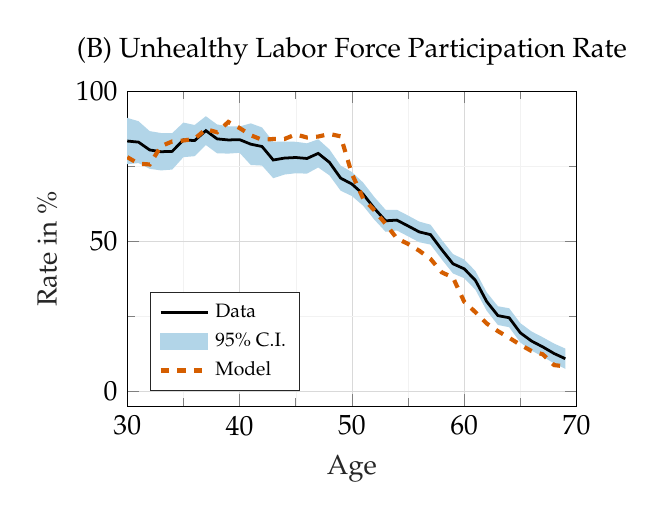
\begin{tikzpicture}
\begin{axis}[%
width=5.706cm,
height=4cm,
at={(0cm,0cm)},
scale only axis,
xmin=30,
xmax=70,
xlabel style={font=\color{white!15!black}},
xlabel={Age},
ymin=-5,
ymax=100,
ylabel style={font=\color{white!15!black}},
ylabel={Rate in \%},
axis background/.style={fill=white},
%title style={font=\bfseries},
title={(B) Unhealthy Labor Force Participation Rate},
legend style={at={(axis cs:32,0)}, anchor=south west, legend cell align=left, align=left, draw=white!15!black, font=\scriptsize},
grid=both,
grid style={line width=0.2pt, draw=gray!30},
minor grid style={line width=0.1pt, draw=gray!10},
minor tick num=1
]

% Main line (lfprlr0) - blue solid line
\addplot [color=black, line width=1pt]
  table[row sep=crcr,y expr=\thisrowno{1}*100]{%
30 0.8339695\\
31 0.830355\\
32 0.8042343\\
33 0.7983715\\
34 0.7995418\\
35 0.8378634\\
36 0.8354884\\
37 0.8686402\\
38 0.8411449\\
39 0.8375973\\
40 0.8386171\\
41 0.8234905\\
42 0.8157026\\
43 0.7707186\\
44 0.7771355\\
45 0.7791017\\
46 0.7758368\\
47 0.7928331\\
48 0.762918\\
49 0.710295\\
50 0.6906397\\
51 0.6569952\\
52 0.6095482\\
53 0.5680759\\
54 0.5703449\\
55 0.5509109\\
56 0.5310219\\
57 0.5219091\\
58 0.4718995\\
59 0.4247883\\
60 0.4079395\\
61 0.3693248\\
62 0.2990521\\
63 0.2519826\\
64 0.2448949\\
65 0.1944834\\
66 0.1670593\\
67 0.1475739\\
68 0.1256826\\
69 0.1083655\\
% 70 0.1681354\\
% 71 0.121358\\
% 72 0.1394618\\
% 73 0.1092736\\
% 74 0.1141775\\
% 75 0.0792269\\
% 76 0.0917666\\
% 77 0.0850947\\
% 78 0.0388536\\
% 79 0.0336195\\
% 80 0.058109\\
% 81 0.016314\\
% 82 0.0270162\\
% 83 -0.0089496\\
% 84 0.0236253\\
% 85 -0.0178846\\
};
\addlegendentry{Data}

% Upper bound (standard error high)
\addplot[name path=upper, draw=none, forget plot] 
  table[row sep=crcr,y expr=\thisrowno{1}*100]{%
30 0.9111052\\
31 0.9001306\\
32 0.8669667\\
33 0.8606798\\
34 0.860257\\
35 0.8955216\\
36 0.8874309\\
37 0.9166927\\
38 0.8892378\\
39 0.8830312\\
40 0.8826435\\
41 0.8928777\\
42 0.8792804\\
43 0.8314206\\
44 0.83197\\
45 0.8315616\\
46 0.8263692\\
47 0.8398106\\
48 0.8062539\\
49 0.7522238\\
50 0.7306355\\
51 0.6956045\\
52 0.6471571\\
53 0.6047442\\
54 0.6048974\\
55 0.5855613\\
56 0.5653728\\
57 0.5550599\\
58 0.5043322\\
59 0.4570315\\
60 0.4391904\\
61 0.4005467\\
62 0.3297285\\
63 0.2832072\\
64 0.2764793\\
65 0.2267636\\
66 0.1990062\\
67 0.1796762\\
68 0.1588332\\
69 0.142154\\
% 70 0.194256\\
% 71 0.1491448\\
% 72 0.1675596\\
% 73 0.1396055\\
% 74 0.1450964\\
% 75 0.1120739\\
% 76 0.1273876\\
% 77 0.1228318\\
% 78 0.0783176\\
% 79 0.0761687\\
% 80 0.1034711\\
% 81 0.0718914\\
% 82 0.080405\\
% 83 0.0504064\\
% 84 0.082339\\
% 85 0.0525297\\
};

% Lower bound (standard error low)
\addplot[name path=lower, draw=none, forget plot] 
  table[row sep=crcr,y expr=\thisrowno{1}*100]{%
30 0.7568338\\
31 0.7605796\\
32 0.7415019\\
33 0.7360631\\
34 0.7388266\\
35 0.7802051\\
36 0.7835459\\
37 0.8205878\\
38 0.7930518\\
39 0.7921634\\
40 0.7945906\\
41 0.7541034\\
42 0.7521245\\
43 0.7100167\\
44 0.7223011\\
45 0.7266418\\
46 0.7253045\\
47 0.7458558\\
48 0.719582\\
49 0.6683661\\
50 0.6506439\\
51 0.618386\\
52 0.5719393\\
53 0.5314076\\
54 0.5357924\\
55 0.5162606\\
56 0.496671\\
57 0.4887584\\
58 0.4394668\\
59 0.3925449\\
60 0.3766887\\
61 0.3381029\\
62 0.2683756\\
63 0.2207581\\
64 0.2133105\\
65 0.1622031\\
66 0.1351124\\
67 0.1154717\\
68 0.092532\\
69 0.0745769\\
% 70 0.1420148\\
% 71 0.0935712\\
% 72 0.111364\\
% 73 0.0789419\\
% 74 0.0832585\\
% 75 0.04638\\
% 76 0.0561455\\
% 77 0.0473576\\
% 78 -0.0006104\\
% 79 -0.0089297\\
% 80 0.012747\\
% 81 -0.0392634\\
% 82 -0.0263728\\
% 83 -0.0683057\\
% 84 -0.0350885\\
% 85 -0.0882989\\
};

% Fill between the paths
\addplot[blue!30] fill between[of=upper and lower];
\addlegendentry{95\% C.I.}

\addplot [color=red, line width=1.5pt, dashed]
  table[row sep=crcr,y expr=\thisrowno{1}*100]{%
30	0.78021978	\\
31	0.75862069	\\
32	0.755813953	\\
33	0.816753927	\\
34	0.832460733	\\
35	0.835680751	\\
36	0.841409692	\\
37	0.873469388	\\
38	0.863117871	\\
39	0.897526502	\\
40	0.877419355	\\
41	0.853293413	\\
42	0.838150289	\\
43	0.840782123	\\
44	0.840848806	\\
45	0.856132075	\\
46	0.845794393	\\
47	0.84893617	\\
48	0.857429719	\\
49	0.849710983	\\
50	0.724738676	\\
51	0.642477876	\\
52	0.602941176	\\
53	0.557959815	\\
54	0.509516837	\\
55	0.490909091	\\
56	0.468253968	\\
57	0.441102757	\\
58	0.396341463	\\
59	0.378787879	\\
60	0.298342541	\\
61	0.263383298	\\
62	0.225774226	\\
63	0.200192493	\\
64	0.178199052	\\
65	0.154620311	\\
66	0.133858268	\\
67	0.122937294	\\
68	0.087027915	\\
69	0.082670906	\\
  };
\addlegendentry{Model}

\end{axis}
\end{tikzpicture} \\[1ex]
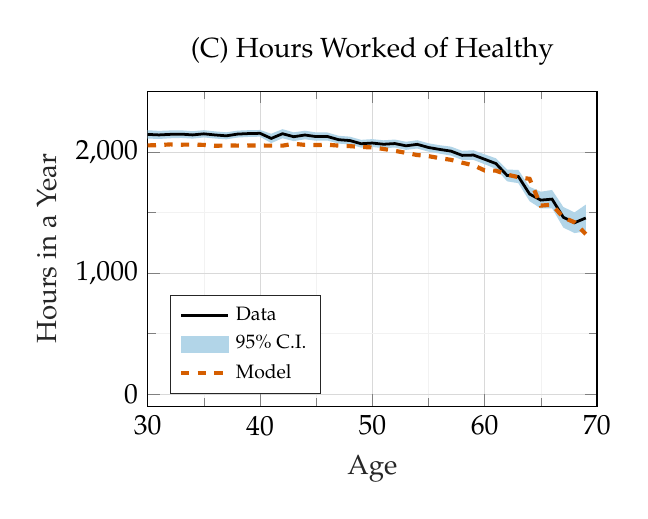
\begin{tikzpicture}
\begin{axis}[%
width=5.706cm,
height=4cm,
at={(0cm,0cm)},
scale only axis,
xmin=30,
xmax=70,
xlabel style={font=\color{white!15!black}},
xlabel={Age},
ymin=-100,
ymax=2500,
ylabel style={font=\color{white!15!black}},
ylabel={Hours in a Year},
axis background/.style={fill=white},
%title style={font=\bfseries},
title={(C) Hours Worked of Healthy},
legend style={at={(axis cs:32,0)}, anchor=south west, legend cell align=left, align=left, draw=white!15!black, font=\scriptsize},
grid=both,
grid style={line width=0.2pt, draw=gray!30},
minor grid style={line width=0.1pt, draw=gray!10},
minor tick num=1
]

% Main line (lfprlr0) - blue solid line
\addplot [color=black, line width=1pt]
  table[row sep=crcr]{%
30 2143.776\\
31 2139.441\\
32 2143.99\\
33 2145.759\\
34 2139.533\\
35 2148.389\\
36 2139.108\\
37 2131.988\\
38 2146.241\\
39 2150.673\\
40 2152.556\\
41 2110.49\\
42 2149.378\\
43 2124.506\\
44 2138.751\\
45 2125.451\\
46 2126.24\\
47 2100.008\\
48 2092.962\\
49 2066.729\\
50 2072.279\\
51 2062.416\\
52 2068.127\\
53 2049.428\\
54 2061.603\\
55 2035.663\\
56 2019.648\\
57 2005.664\\
58 1970.462\\
59 1973.028\\
60 1938.318\\
61 1903.091\\
62 1804.867\\
63 1795.704\\
64 1651.485\\
65 1601.154\\
66 1609.429\\
67 1459.81\\
68 1414.398\\
69 1453.738\\
% 70 0.1681354\\
% 71 0.121358\\
% 72 0.1394618\\
% 73 0.1092736\\
% 74 0.1141775\\
% 75 0.0792269\\
% 76 0.0917666\\
% 77 0.0850947\\
% 78 0.0388536\\
% 79 0.0336195\\
% 80 0.058109\\
% 81 0.016314\\
% 82 0.0270162\\
% 83 -0.0089496\\
% 84 0.0236253\\
% 85 -0.0178846\\
};
\addlegendentry{Data}

% Upper bound (standard error high)
\addplot[name path=upper, draw=none, forget plot] 
  table[row sep=crcr]{%
30 2178.159\\
31 2172.766\\
32 2176.314\\
33 2177.107\\
34 2170.112\\
35 2178.354\\
36 2168.583\\
37 2161.071\\
38 2174.72\\
39 2178.67\\
40 2180.178\\
41 2149.47\\
42 2186.848\\
43 2160.524\\
44 2174.171\\
45 2159.688\\
46 2159.397\\
47 2132.224\\
48 2125.058\\
49 2098.81\\
50 2104.721\\
51 2095.058\\
52 2101.074\\
53 2082.783\\
54 2095.726\\
55 2070.287\\
56 2054.273\\
57 2042.598\\
58 2008.204\\
59 2012.989\\
60 1978.96\\
61 1946.624\\
62 1853.525\\
63 1850.296\\
64 1710.904\\
65 1670.316\\
66 1684.934\\
67 1544.774\\
68 1499.869\\
69 1563.532\\
% 70 0.194256\\
% 71 0.1491448\\
% 72 0.1675596\\
% 73 0.1396055\\
% 74 0.1450964\\
% 75 0.1120739\\
% 76 0.1273876\\
% 77 0.1228318\\
% 78 0.0783176\\
% 79 0.0761687\\
% 80 0.1034711\\
% 81 0.0718914\\
% 82 0.080405\\
% 83 0.0504064\\
% 84 0.082339\\
% 85 0.0525297\\
};

% Lower bound (standard error low)
\addplot[name path=lower, draw=none, forget plot] 
  table[row sep=crcr]{%
30 2109.393\\
31 2106.114\\
32 2111.666\\
33 2114.411\\
34 2108.954\\
35 2118.425\\
36 2109.633\\
37 2102.906\\
38 2117.763\\
39 2122.676\\
40 2124.933\\
41 2071.511\\
42 2111.908\\
43 2088.489\\
44 2103.332\\
45 2091.215\\
46 2093.082\\
47 2067.791\\
48 2060.867\\
49 2034.649\\
50 2039.836\\
51 2029.775\\
52 2035.18\\
53 2016.075\\
54 2027.478\\
55 2001.039\\
56 1985.023\\
57 1968.731\\
58 1932.72\\
59 1933.067\\
60 1897.676\\
61 1859.56\\
62 1756.209\\
63 1741.111\\
64 1592.067\\
65 1531.993\\
66 1533.925\\
67 1374.848\\
68 1328.928\\
69 1343.943\\
% 70 0.1420148\\
% 71 0.0935712\\
% 72 0.111364\\
% 73 0.0789419\\
% 74 0.0832585\\
% 75 0.04638\\
% 76 0.0561455\\
% 77 0.0473576\\
% 78 -0.0006104\\
% 79 -0.0089297\\
% 80 0.012747\\
% 81 -0.0392634\\
% 82 -0.0263728\\
% 83 -0.0683057\\
% 84 -0.0350885\\
% 85 -0.0882989\\
};

% Fill between the paths
\addplot[blue!30] fill between[of=upper and lower];
\addlegendentry{95\% C.I.}

\addplot [color=red, line width=1.5pt, dashed]
  table[row sep=crcr,y expr=\thisrowno{1}*10000]{%
30	0.205295842	\\
31	0.205526395	\\
32	0.206114898	\\
33	0.205867054	\\
34	0.206015468	\\
35	0.20569313	\\
36	0.204987772	\\
37	0.20519013	\\
38	0.205139498	\\
39	0.20520453	\\
40	0.205179348	\\
41	0.205100805	\\
42	0.205075625	\\
43	0.206607399	\\
44	0.205723535	\\
45	0.205571237	\\
46	0.205841736	\\
47	0.205101708	\\
48	0.204669166	\\
49	0.203989067	\\
50	0.203620959	\\
51	0.202356117	\\
52	0.200801548	\\
53	0.199159249	\\
54	0.197332475	\\
55	0.196406289	\\
56	0.194772139	\\
57	0.193386441	\\
58	0.190991453	\\
59	0.188867887	\\
60	0.184614878	\\
61	0.18442398	\\
62	0.181224373	\\
63	0.17900882	\\
64	0.177673307	\\
65	0.155600545	\\
66	0.156352262	\\
67	0.145757376	\\
68	0.14182622	\\
69	0.132082454	\\
  };
\addlegendentry{Model}

\end{axis}
\end{tikzpicture} & 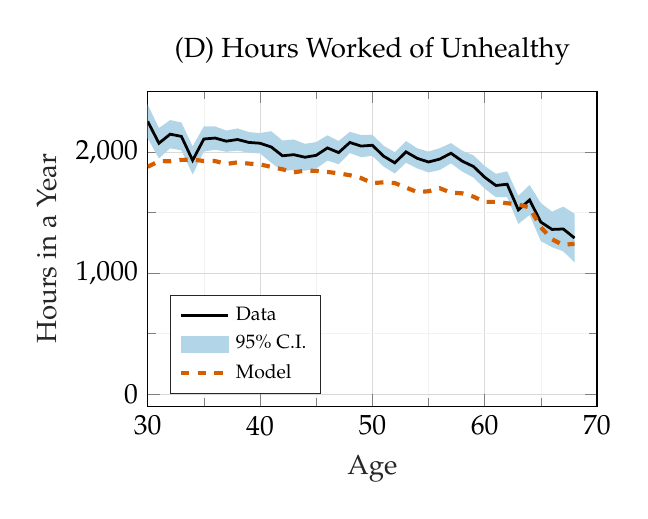
\begin{tikzpicture}
\begin{axis}[%
width=5.706cm,
height=4cm,
at={(0cm,0cm)},
scale only axis,
xmin=30,
xmax=70,
xlabel style={font=\color{white!15!black}},
xlabel={Age},
ymin=-100,
ymax=2500,
ylabel style={font=\color{white!15!black}},
ylabel={Hours in a Year},
axis background/.style={fill=white},
%title style={font=\bfseries},
title={(D) Hours Worked of Unhealthy},
legend style={at={(axis cs:32,0)}, anchor=south west, legend cell align=left, align=left, draw=white!15!black, font=\scriptsize},
grid=both,
grid style={line width=0.2pt, draw=gray!30},
minor grid style={line width=0.1pt, draw=gray!10},
minor tick num=1
]

% Main line (lfprlr0) - blue solid line
\addplot [color=black, line width=1pt]
  table[row sep=crcr]{%
30 2251.003\\
31 2070.796\\
32 2145.518\\
33 2127.26\\
34 1929.438\\
35 2105.717\\
36 2113.603\\
37 2087.747\\
38 2101.477\\
39 2077.569\\
40 2070.723\\
41 2039.721\\
42 1967.084\\
43 1976.383\\
44 1955.178\\
45 1970.855\\
46 2031.943\\
47 1993.444\\
48 2077.078\\
49 2047.202\\
50 2053.981\\
51 1964.306\\
52 1908.962\\
53 1999.357\\
54 1945.93\\
55 1915.884\\
56 1939.809\\
57 1988.51\\
58 1923.068\\
59 1878.974\\
60 1790.333\\
61 1721.866\\
62 1732.454\\
63 1520.456\\
64 1602.545\\
65 1420.01\\
66 1359.269\\
67 1362.846\\
68 1288.484\\
%69 1807.444\\
};
\addlegendentry{Data}

% Upper bound (standard error high)
\addplot[name path=upper, draw=none, forget plot] 
  table[row sep=crcr]{%
30 2390.313\\
31 2195.989\\
32 2262.114\\
33 2242.274\\
34 2044.891\\
35 2209.809\\
36 2209.399\\
37 2175.672\\
38 2193.126\\
39 2162.5\\
40 2154.901\\
41 2169.775\\
42 2092.91\\
43 2101.938\\
44 2065.909\\
45 2080.342\\
46 2136.135\\
47 2089.37\\
48 2164.87\\
49 2138.22\\
50 2141.137\\
51 2050.262\\
52 1996.334\\
53 2089.142\\
54 2029.02\\
55 2001.805\\
56 2030.229\\
57 2071.969\\
58 2009.097\\
59 1970.57\\
60 1883.818\\
61 1818.307\\
62 1838.893\\
63 1636.977\\
64 1726.484\\
65 1577.326\\
66 1505.979\\
67 1547.479\\
68 1488.87\\
%69 2023.508\\
};

% Lower bound (standard error low)
\addplot[name path=lower, draw=none, forget plot] 
  table[row sep=crcr]{%
30 2111.693\\
31 1945.602\\
32 2028.922\\
33 2012.246\\
34 1813.987\\
35 2001.627\\
36 2017.806\\
37 1999.822\\
38 2009.828\\
39 1992.638\\
40 1986.546\\
41 1909.665\\
42 1841.258\\
43 1850.828\\
44 1844.447\\
45 1861.37\\
46 1927.751\\
47 1897.518\\
48 1989.286\\
49 1956.185\\
50 1966.826\\
51 1878.35\\
52 1821.59\\
53 1909.572\\
54 1862.839\\
55 1829.962\\
56 1849.388\\
57 1905.05\\
58 1837.039\\
59 1787.379\\
60 1696.848\\
61 1625.426\\
62 1626.016\\
63 1403.934\\
64 1478.605\\
65 1262.693\\
66 1212.56\\
67 1178.212\\
68 1088.099\\
%69 1591.381\\
};

% Fill between the paths
\addplot[blue!30] fill between[of=upper and lower];
\addlegendentry{95\% C.I.}

\addplot [color=red, line width=1.5pt, dashed]
  table[row sep=crcr,y expr=\thisrowno{1}*10000]{%
30	0.187588598	\\
31	0.192390747	\\
32	0.192173911	\\
33	0.193311463	\\
34	0.193609164	\\
35	0.192411646	\\
36	0.192379998	\\
37	0.189944085	\\
38	0.1912981	\\
39	0.190264372	\\
40	0.189650774	\\
41	0.187501925	\\
42	0.185557516	\\
43	0.183047389	\\
44	0.184401807	\\
45	0.184252797	\\
46	0.183396436	\\
47	0.182204533	\\
48	0.180671643	\\
49	0.178315392	\\
50	0.174125435	\\
51	0.17480496	\\
52	0.17421259	\\
53	0.170458916	\\
54	0.166733425	\\
55	0.167446385	\\
56	0.169953485	\\
57	0.166272829	\\
58	0.165723098	\\
59	0.162980792	\\
60	0.158670974	\\
61	0.158646658	\\
62	0.157559775	\\
63	0.156468874	\\
64	0.154061234	\\
65	0.137729406	\\
66	0.127735163	\\
67	0.123107954	\\
68	0.124116753	\\
%69	0.116047467	\\
  };
\addlegendentry{Model}

\end{axis}
\end{tikzpicture}
\end{tabular}
\tabnotes{\textit{Notes:} Panels A and B show labor force participation rates (percent) of healthy individuals ($h=0$) and unhealthy individuals (poor health or disability, $h\in\{1,2\}$); panels C and D show annual hours worked conditional on participation for the same groups. An individual participates if she works more than 800 hours in the year. Solid lines are data profiles estimated from the Panel Study of Income Dynamics as described in Appendix~\ref{app:msm}, shaded areas are 95\% confidence intervals, and dashed lines are profiles simulated from the model at the estimates of \autoref{tab:estimates}. All profiles are targeted in the estimation.}
\end{figure}

\autoref{fig:fit_assets} shows the wealth and reentry profiles. The model tracks mean assets until the early 50s. It overstates median assets in the 30s and 40s, when the data median lies well below the data mean: wealth in the data is more concentrated than in a model in which households differ only in their shocks. After the mid-50s, simulated mean and median wealth fall below the data. The divergence arises because the model has accidental bequests but no bequest motive, which typically raises saving at older ages \citep{Denardi2010,lockwood2018incidental}. We abstract from bequest motives to keep the model comparable with the life-cycle taxation literature \citep{farhi2013insurance,golosov2016redistribution,Stantcheva2017} and with our companion normative analysis. As a result, older households in the model rely more on Social Security income and the consumption floor than their counterparts in the data. A specification with separable logarithmic utility over consumption, estimated in Appendix~\ref{app:logpref}, fits old-age assets better but participation worse.

Reentry rates are low in the data, below 5 percent at every age, and the model generates no reentry. The large estimated reentry cost reconciles the model with this fact, and makes exit from the labor force effectively absorbing. Overall, the estimated model reproduces the patterns of labor supply and saving over the life cycle through which retirement reforms operate, which makes it a useful laboratory for measuring their welfare and fiscal effects. \citet{NdiayeYu2026frot} use the same estimated economy to quantify the channels---fixed costs of work, health-related productivity losses, and differential mortality---through which health shapes retirement.

\begin{figure}[!htbp]
\centering
\caption{Data and Simulated Profiles: Assets and Reentry}\label{fig:fit_assets}
\vspace{0.5em}
% Asset panels: corrected 2026 re-simulation at the same estimates (FROT figures/abdou/*_c.tex); reentry panel: FROT figures/abdou/h800_reentry_edit.tex. Copied verbatim.
\begin{tabular}{@{}c@{\hspace{1.5em}}c@{}}
% EDITED (MVPF paper, revision pass): axis range and legend placement only: ymin/ymax -5/10 -> -1/5; legend moved to the upper left (axis cs:31,4.8, anchor north west). Data unchanged.
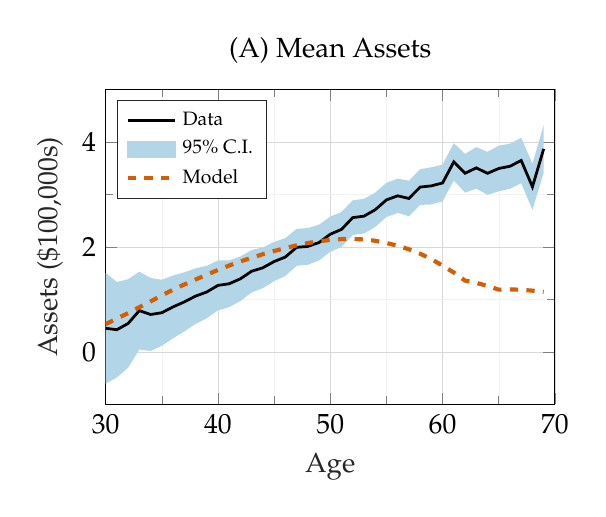
\begin{tikzpicture}
\begin{axis}[%
width=5.706cm,
height=4cm,
at={(0cm,0cm)},
scale only axis,
xmin=30,
xmax=70,
xlabel style={font=\color{white!15!black}},
xlabel={Age},
ymin=-1,
ymax=5,
ylabel style={font=\color{white!15!black}},
ylabel={Assets (\$100{,}000s)},
axis background/.style={fill=white},
%title style={font=\bfseries},
title={(A) Mean Assets},
legend style={at={(axis cs:31,4.8)}, anchor=north west, legend cell align=left, align=left, draw=white!15!black, font=\scriptsize},
grid=both,
grid style={line width=0.2pt, draw=gray!30},
minor grid style={line width=0.1pt, draw=gray!10},
minor tick num=1
]

% Main line (lfprlr0) - blue solid line
\addplot [color=black, line width=1pt]
  table[row sep=crcr]{%, y expr=\thisrowno{1}*100]{%
30	0.44883396	\\
31	0.42199558	\\
32	0.54018803	\\
33	0.78561033	\\
34	0.71175356	\\
35	0.74541797	\\
36	0.85600565	\\
37	0.95088265	\\
38	1.0613716	\\
39	1.1398318	\\
40	1.2659439	\\
41	1.2972758	\\
42	1.3919758	\\
43	1.535846	\\
44	1.6013677	\\
45	1.7205047	\\
46	1.8064766	\\
47	1.9908018	\\
48	2.0085264	\\
49	2.0823645	\\
50	2.2407959	\\
51	2.3326437	\\
52	2.556798	\\
53	2.5850001	\\
54	2.7065999	\\
55	2.8947089	\\
56	2.9723681	\\
57	2.9223428	\\
58	3.1388551	\\
59	3.1621034	\\
60	3.2175482	\\
61	3.620027	\\
62	3.4022311	\\
63	3.50429	\\
64	3.4009493	\\
65	3.4932815	\\
66	3.5353909	\\
67	3.6457606	\\
68	3.1442149	\\
69	3.8660995	\\
};
\addlegendentry{Data}

% Upper bound (standard error high)
\addplot[name path=upper, draw=none, forget plot] 
  table[row sep=crcr]{%,y expr=\thisrowno{1}*100]{%
%age1	plus2se	
30	1.5034447	\\
31	1.3318214	\\
32	1.3825211	\\
33	1.5269781	\\
34	1.4072133	\\
35	1.3745624	\\
36	1.4530003	\\
37	1.5145966	\\
38	1.5909592	\\
39	1.6398946	\\
40	1.7404519	\\
41	1.742667	\\
42	1.8167697	\\
43	1.9404281	\\
44	1.9883948	\\
45	2.0936916	\\
46	2.1680532	\\
47	2.3425176	\\
48	2.3583419	\\
49	2.4231668	\\
50	2.5766613	\\
51	2.6659567	\\
52	2.8871246	\\
53	2.9148088	\\
54	3.0332248	\\
55	3.2218368	\\
56	3.2981602	\\
57	3.260209	\\
58	3.4790351	\\
59	3.5159971	\\
60	3.5670526	\\
61	3.9753495	\\
62	3.7715802	\\
63	3.9004755	\\
64	3.8095388	\\
65	3.92889	\\
66	3.964179	\\
67	4.080106	\\
68	3.5837879	\\
69	4.3190544	\\
};

% Lower bound (standard error low)
\addplot[name path=lower, draw=none, forget plot] 
  table[row sep=crcr]{%,y expr=\thisrowno{1}*100]{%
%age1	minus2se	
30	-0.60577681	\\
31	-0.48783214	\\
32	-0.3021432	\\
33	0.04424252	\\
34	0.01629566	\\
35	0.11627356	\\
36	0.25901103	\\
37	0.38716866	\\
38	0.53178403	\\
39	0.63977097	\\
40	0.79143593	\\
41	0.85188656	\\
42	0.96718204	\\
43	1.1312658	\\
44	1.2143407	\\
45	1.347316	\\
46	1.4449018	\\
47	1.639086	\\
48	1.6587109	\\
49	1.7415622	\\
50	1.9049305	\\
51	1.9993306	\\
52	2.2264713	\\
53	2.2551913	\\
54	2.379975	\\
55	2.567581	\\
56	2.6465741	\\
57	2.5844784	\\
58	2.798675	\\
59	2.8082117	\\
60	2.8680457	\\
61	3.2647044	\\
62	3.032882	\\
63	3.1081044	\\
64	2.9923581	\\
65	3.057673	\\
66	3.1066009	\\
67	3.2114152	\\
68	2.7046419	\\
69	3.4131445	\\
};

% Fill between the paths
\addplot[blue!30] fill between[of=upper and lower];
\addlegendentry{95\% C.I.}

\addplot [color=red, line width=1.5pt, dashed]
  table[row sep=crcr]{%,y expr=\thisrowno{1}*100]{%
%age1	means	
30	0.528489028	\\
31	0.633230367	\\
32	0.739050697	\\
33	0.849863772	\\
34	0.960606134	\\
35	1.073980097	\\
36	1.183967902	\\
37	1.282999342	\\
38	1.377252345	\\
39	1.468645169	\\
40	1.559869506	\\
41	1.644474279	\\
42	1.722001208	\\
43	1.791600174	\\
44	1.860443712	\\
45	1.9207767	\\
46	1.976688014	\\
47	2.028959309	\\
48	2.072432524	\\
49	2.106475279	\\
50	2.131889566	\\
51	2.14796458	\\
52	2.151009084	\\
53	2.141524019	\\
54	2.116176358	\\
55	2.073609879	\\
56	2.020872452	\\
57	1.953956345	\\
58	1.870023323	\\
59	1.766523005	\\
60	1.641839629	\\
61	1.511149276	\\
62	1.357284975	\\
63	1.314517195	\\
64	1.255450127	\\
65	1.185440906	\\
66	1.189826815	\\
67	1.183263906	\\
68	1.165725954	\\
69	1.140764718	\\
  };
\addlegendentry{Model};

\end{axis}
\end{tikzpicture} & % EDITED (MVPF paper, revision pass): axis range and legend placement only: ymin/ymax -5/10 -> -1/5; legend moved to the upper left (axis cs:31,4.8, anchor north west). Data unchanged.
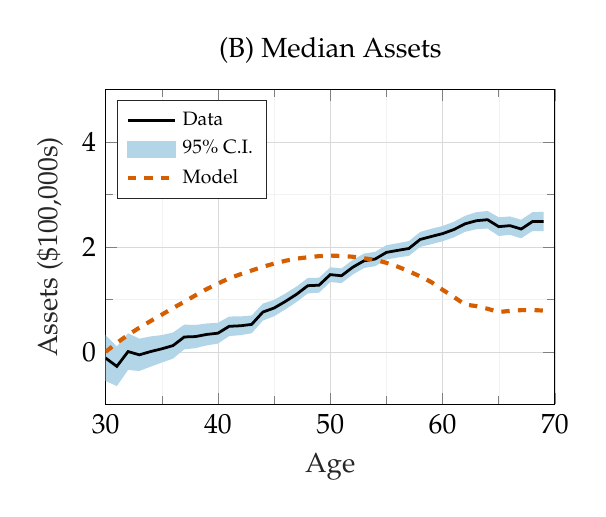
\begin{tikzpicture}
\begin{axis}[%
width=5.706cm,
height=4cm,
at={(0cm,0cm)},
scale only axis,
xmin=30,
xmax=70,
xlabel style={font=\color{white!15!black}},
xlabel={Age},
ymin=-1,
ymax=5,
ylabel style={font=\color{white!15!black}},
ylabel={Assets (\$100{,}000s)},
axis background/.style={fill=white},
%title style={font=\bfseries},
title={(B) Median Assets},
legend style={at={(axis cs:31,4.8)}, anchor=north west, legend cell align=left, align=left, draw=white!15!black, font=\scriptsize},
grid=both,
grid style={line width=0.2pt, draw=gray!30},
minor grid style={line width=0.1pt, draw=gray!10},
minor tick num=1
]

% Main line (lfprlr0) - blue solid line
\addplot [color=black, line width=1pt]
  table[row sep=crcr]{%, y expr=\thisrowno{1}*100]{%
30	-0.11895441	\\
31	-0.27639282	\\
32	0.0054679	\\
33	-0.05680846	\\
34	0.00530582	\\
35	0.05775673	\\
36	0.11935496	\\
37	0.283448	\\
38	0.29103227	\\
39	0.3317854	\\
40	0.3554958	\\
41	0.48654667	\\
42	0.49660314	\\
43	0.5230298	\\
44	0.75761317	\\
45	0.83516986	\\
46	0.95970209	\\
47	1.09713	\\
48	1.2602245	\\
49	1.2697649	\\
50	1.4709074	\\
51	1.4499263	\\
52	1.6115453	\\
53	1.7346132	\\
54	1.768639	\\
55	1.894712	\\
56	1.932978	\\
57	1.9691985	\\
58	2.1408199	\\
59	2.198014	\\
60	2.2522161	\\
61	2.329607	\\
62	2.4388831	\\
63	2.4980613	\\
64	2.5174607	\\
65	2.3850927	\\
66	2.403937	\\
67	2.3398796	\\
68	2.4810502	\\
69	2.4844838	\\
};
\addlegendentry{Data}

% Upper bound (standard error high)
\addplot[name path=upper, draw=none, forget plot] 
  table[row sep=crcr]{%,y expr=\thisrowno{1}*100]{%
30	0.31699318	\\
31	0.10011389	\\
32	0.35445438	\\
33	0.2506089	\\
34	0.29365724	\\
35	0.31921015	\\
36	0.36788288	\\
37	0.51851016	\\
38	0.51206232	\\
39	0.54050287	\\
40	0.55375253	\\
41	0.6729007	\\
42	0.67474134	\\
43	0.69266526	\\
44	0.9196122	\\
45	0.99146252	\\
46	1.1109516	\\
47	1.2443443	\\
48	1.4066153	\\
49	1.4124912	\\
50	1.6117372	\\
51	1.5897184	\\
52	1.74986	\\
53	1.8723206	\\
54	1.9050796	\\
55	2.0317431	\\
56	2.069126	\\
57	2.1103524	\\
58	2.2830432	\\
59	2.3452282	\\
60	2.3976214	\\
61	2.4770057	\\
62	2.5911442	\\
63	2.660554	\\
64	2.6842085	\\
65	2.563393	\\
66	2.5792043	\\
67	2.5160896	\\
68	2.66001	\\
69	2.6677378	\\
};

% Lower bound (standard error low)
\addplot[name path=lower, draw=none, forget plot] 
  table[row sep=crcr]{%,y expr=\thisrowno{1}*100]{%
30	-0.55490014	\\
31	-0.65290139	\\
32	-0.34352043	\\
33	-0.36422581	\\
34	-0.28304559	\\
35	-0.20369669	\\
36	-0.12917297	\\
37	0.04838584	\\
38	0.07000223	\\
39	0.12306792	\\
40	0.15724093	\\
41	0.30019264	\\
42	0.31846681	\\
43	0.35339433	\\
44	0.595616	\\
45	0.6788772	\\
46	0.80845444	\\
47	0.94991389	\\
48	1.1138318	\\
49	1.1270405	\\
50	1.3300777	\\
51	1.3101343	\\
52	1.4732306	\\
53	1.5969077	\\
54	1.6321967	\\
55	1.757679	\\
56	1.79683	\\
57	1.8280445	\\
58	1.9985966	\\
59	2.0507979	\\
60	2.1068127	\\
61	2.1822064	\\
62	2.2866238	\\
63	2.3355686	\\
64	2.3507148	\\
65	2.2067924	\\
66	2.2286696	\\
67	2.1636714	\\
68	2.3020905	\\
69	2.3012316	\\
};

% Fill between the paths
\addplot[blue!30] fill between[of=upper and lower];
\addlegendentry{95\% C.I.}

\addplot [color=red, line width=1.5pt, dashed]
  table[row sep=crcr]{%,y expr=\thisrowno{1}*100]{%
30	0	\\
31	0.169848043	\\
32	0.324047755	\\
33	0.458929333	\\
34	0.58588607	\\
35	0.708232142	\\
36	0.834945068	\\
37	0.953362006	\\
38	1.077344885	\\
39	1.195834593	\\
40	1.301419969	\\
41	1.400786892	\\
42	1.478278188	\\
43	1.5495248	\\
44	1.620944859	\\
45	1.681464662	\\
46	1.734871359	\\
47	1.775941666	\\
48	1.80198262	\\
49	1.82314822	\\
50	1.833265634	\\
51	1.827195632	\\
52	1.811864454	\\
53	1.782321958	\\
54	1.75352012	\\
55	1.695517106	\\
56	1.623180416	\\
57	1.535345572	\\
58	1.437292072	\\
59	1.328316533	\\
60	1.182584964	\\
61	1.045613071	\\
62	0.90142578	\\
63	0.871179625	\\
64	0.820927595	\\
65	0.758226595	\\
66	0.780832251	\\
67	0.794580994	\\
68	0.797297309	\\
69	0.785855602	\\
  };
\addlegendentry{Model}

\end{axis}
\end{tikzpicture}
\end{tabular}\\[1ex]
% EDITED (MVPF paper, revision pass): axis range and legend placement only: ymin/ymax -5/100 -> -0.5/10; legend moved to the upper left (axis cs:31,9.6, anchor north west). Data unchanged.
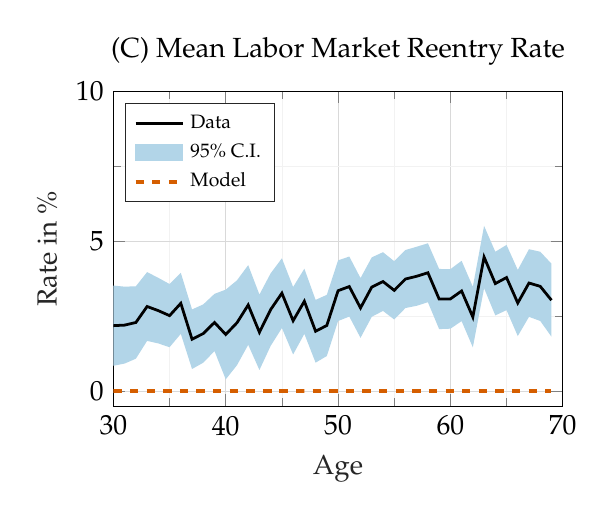
\begin{tikzpicture}
\begin{axis}[%
width=5.706cm,
height=4cm,
at={(0cm,0cm)},
scale only axis,
xmin=30,
xmax=70,
xlabel style={font=\color{white!15!black}},
xlabel={Age},
ymin=-0.5,
ymax=10,
ylabel style={font=\color{white!15!black}},
ylabel={Rate in \%},
axis background/.style={fill=white},
%title style={font=\bfseries},
title={(C) Mean Labor Market Reentry Rate},
legend style={at={(axis cs:31,9.6)}, anchor=north west, legend cell align=left, align=left, draw=white!15!black, font=\scriptsize},
grid=both,
grid style={line width=0.2pt, draw=gray!30},
minor grid style={line width=0.1pt, draw=gray!10},
minor tick num=1
]

% Main line (lfprlr0) - blue solid line
\addplot [color=black, line width=1pt]
  table[row sep=crcr]{%, y expr=\thisrowno{1}*100]{%
30		2.18517	\\
31		2.20335	\\
32		2.29117	\\
33		2.82388	\\
34		2.68548	\\
35		2.51887	\\
36		2.93026	\\
37		1.73287	\\
38		1.92231	\\
39		2.29121	\\
40		1.89049	\\
41		2.28087	\\
42		2.87458	\\
43		1.96387	\\
44		2.72082	\\
45		3.2679	\\
46		2.34941	\\
47		2.99802	\\
48		1.99764	\\
49		2.19266	\\
50		3.35012	\\
51		3.48878	\\
52		2.77504	\\
53		3.4707	\\
54		3.65526	\\
55		3.36258	\\
56		3.73983	\\
57		3.83127	\\
58		3.94909	\\
59		3.07238	\\
60		3.07621	\\
61		3.34096	\\
62		2.47159	\\
63		4.47199	\\
64		3.58776	\\
65		3.78918	\\
66		2.94066	\\
67		3.6062	\\
68		3.49552	\\
69		3.03359	\\
};
\addlegendentry{Data}

% Upper bound (standard error high)
\addplot[name path=upper, draw=none, forget plot] 
  table[row sep=crcr]{%,y expr=\thisrowno{1}*100]{%
30	3.52233	\\
31	3.48453	\\
32	3.49816	\\
33	3.97023	\\
34	3.77836	\\
35	3.57231	\\
36	3.94685	\\
37	2.7254	\\
38	2.89398	\\
39	3.24539	\\
40	3.38602	\\
41	3.69561	\\
42	4.20236	\\
43	3.22092	\\
44	3.9306	\\
45	4.43054	\\
46	3.47433	\\
47	4.08391	\\
48	3.0435	\\
49	3.21237	\\
50	4.36057	\\
51	4.48915	\\
52	3.77012	\\
53	4.46092	\\
54	4.63324	\\
55	4.33491	\\
56	4.7065	\\
57	4.81561	\\
58	4.93147	\\
59	4.07507	\\
60	4.06802	\\
61	4.34707	\\
62	3.48016	\\
63	5.51106	\\
64	4.64884	\\
65	4.87608	\\
66	4.04335	\\
67	4.7332	\\
68	4.6497	\\
69	4.25052	\\
};

% Lower bound (standard error low)
\addplot[name path=lower, draw=none, forget plot] 
  table[row sep=crcr]{%,y expr=\thisrowno{1}*100]{%
30	0.84801	\\
31	0.92216	\\
32	1.08417	\\
33	1.67754	\\
34	1.5926	\\
35	1.46544	\\
36	1.91367	\\
37	0.74035	\\
38	0.95064	\\
39	1.33704	\\
40	0.39496	\\
41	0.86613	\\
42	1.5468	\\
43	0.70682	\\
44	1.51103	\\
45	2.10526	\\
46	1.2245	\\
47	1.91214	\\
48	0.95177	\\
49	1.17295	\\
50	2.33967	\\
51	2.48841	\\
52	1.77995	\\
53	2.48048	\\
54	2.67729	\\
55	2.39025	\\
56	2.77315	\\
57	2.84692	\\
58	2.96672	\\
59	2.06969	\\
60	2.08439	\\
61	2.33486	\\
62	1.46303	\\
63	3.43292	\\
64	2.52668	\\
65	2.70228	\\
66	1.83796	\\
67	2.47919	\\
68	2.34135	\\
69	1.81667	\\
};

% Fill between the paths
\addplot[blue!30] fill between[of=upper and lower];
\addlegendentry{95\% C.I.}

\addplot [color=red, line width=1.5pt, dashed]
  table[row sep=crcr]{%
30	0	\\
31	0	\\
32	0	\\
33	0	\\
34	0	\\
35	0	\\
36	0	\\
37	0	\\
38	0	\\
39	0	\\
40	0	\\
41	0	\\
42	0	\\
43	0	\\
44	0	\\
45	0	\\
46	0	\\
47	0	\\
48	0	\\
49	0	\\
50	0	\\
51	0	\\
52	0	\\
53	0	\\
54	0	\\
55	0	\\
56	0	\\
57	0	\\
58	0	\\
59	0	\\
60	0	\\
61	0	\\
62	0	\\
63	0	\\
64	0	\\
65	0	\\
66	0	\\
67	0	\\
68	0	\\
69	0	\\
  };
\addlegendentry{Model}

\end{axis}
\end{tikzpicture}
\tabnotes{\textit{Notes:} Panels A and B show mean and median nonpension assets (hundreds of thousands of 2016 dollars); panel C shows the mean labor market reentry rate (percent). Solid lines are data profiles estimated from the Panel Study of Income Dynamics as described in Appendix~\ref{app:msm}, shaded areas are 95\% confidence intervals, and dashed lines are profiles simulated from the model at the estimates of \autoref{tab:estimates}. All profiles are targeted in the estimation. Asset and reentry profiles are not conditioned on health.}
\end{figure}

% ============================================================================
%  Section 4: Measuring the Value of Retirement Reforms
%  Sources: FROT 2025_sub/12_app_quant.tex ("Construction of Reforms",
%  "Construction of Outcomes"), 2025_sub/7_policy_reforms.tex; blueprint sec. 7.
%  Derivations: Appendix E (sections/E_derivations.tex).
% ============================================================================
\section{Measuring the Value of Retirement Reforms}\label{sec:framework}

The marginal value of public funds (MVPF) of a policy is the willingness to pay of its beneficiaries divided by its net cost to the government, including the fiscal externalities of the behavioral responses it induces \citep{hendren2016policy,hendren2020unified}. For a life-cycle policy, both objects must be measured over the whole life cycle: the willingness to pay before individuals know the health and earnings histories that determine what they receive, and the net cost across every program the policy affects, including responses that occur decades before or after the reformed rule applies. This section defines both objects in our model, relates their ratio to the sufficient-statistics analysis of pension reform, and derives the accounting identity that governs the fiscal effects of claiming-age reforms.

\subsection{Reforms}

A reform is a permanent change in the policy rules of Section~\ref{sec:model}, announced before the cohort enters the model at age 30 and in force over its entire life; the status quo is the estimated economy of Section~\ref{sec:estimation}. For each reform, we solve the individual's problem \eqref{eq:value} under the new rules and simulate the cohort from the same initial distribution. Because the reform is known from age 30, its effects include responses long before the reformed rule applies: a worker who expects a more generous benefit formula adjusts her hours at 35, when her earnings enter her AIME, as well as her exit at 63.

We study 66 reforms in five families, constructed in Appendix~\ref{app:reforms}. The first family (17 reforms) changes the claiming-age adjustment $\alpha(\cdot)$ of Section~\ref{sec:model_ss}. Reforms AN1--AN3 raise the NRA from 65 to 66, 67, and 68, which shifts the entire schedule of benefits by claiming age to the right. Reforms AD1--AD5 raise the DRC from 4.5 percent to 8, 8.5, 9, 9.5, and 10 percent and leave the reductions for early claiming unchanged. Reforms AL1--AL9 make the adjustment symmetric around the NRA of 65: the benefit changes by $x$ percent of the PIA for each year by which the claim precedes or follows the NRA, with $x$ from 7 to 15 percent. \autoref{fig:schedules} and \autoref{tab:schedules} display the schedules. The second family (39 reforms) raises the replacement rates of the benefit formula \eqref{eq:pia}. Reforms P1.1--P1.9 raise the first rate from 0.90 to 0.91, \ldots, 0.99; with the first rate at 0.99, reforms P2.0--P2.9 raise the second rate from 0.32 in ten steps of 1 percent of its initial value, to 0.3232, \ldots, 0.352; and with the second rate at 0.352, reforms P3.0--P3.9 raise the third rate from 0.15 in the same proportional steps, to 0.1515, \ldots, 0.165. Reforms L0--L9 raise all three rates in proportion, by 1 to 10 percent.

The third family (two reforms) raises the share of medical expenditures after age 65 that Medicare covers by 20 percentage points, for all individuals (Part A) or for labor market nonparticipants (Part B), relative to a baseline in which coverage rates vary with health and working status as in the MEPS. The fourth family (five reforms) lowers income taxes in old age: reforms I1--I5 raise the level parameter of the tax function \eqref{eq:tax} from $\lambda_t$ to $\lambda_t+x(t-61)$ at ages $t\geq 62$, with $x$ from 1 to 5 percent, which raises after-tax income at every income level by the proportion $x(t-61)/\lambda_t$. The fifth family (three reforms) raises the net return on assets at every age by 0.2, 0.4, and 0.8 percentage points; the largest subsidy sets the net return equal to the pretax return $r_f$. All reforms except the savings subsidies change benefits, coverage, or taxes only from age 62, the earliest claiming age; this distinction governs the conversion of welfare into dollars (Section~\ref{sec:fw_mvpf}).

We also remove the existing instruments one at a time: D1 sets Social Security benefits to zero, D2 compares the status quo with full coverage of medical expenditures after age 65, D3 sets the net return equal to the pretax return, D4 eliminates the income tax, and D5 eliminates DI. These experiments are not financed, and we report only their welfare effects (Section~\ref{sec:results_elim}).

\subsection{Welfare}\label{sec:fw_welfare}

Let $\bar V^{0}$ be the average over simulated individuals of the value at age 30, $V_{30}(X_{30})$, in the status quo, and $\bar V^{1}$ the same average under a reform. Flow utility \eqref{eq:utility} is homogeneous of degree $\gamma(1-\nu)$ in consumption: multiplying consumption by $e^{x}$ at every age and in every state, with leisure unchanged, multiplies flow utility by $e^{\gamma(1-\nu)x}$, and therefore multiplies each individual's expected lifetime utility, and their average $\bar V^{0}$, by the same factor. The consumption-equivalent welfare change (CE) of a reform is the $x$ that solves $\bar V^{1}=e^{\gamma(1-\nu)x}\,\bar V^{0}$:
\begin{equation}\label{eq:ce}
\mathit{CE}=\frac{\ln\big(\bar V^{1}/\bar V^{0}\big)}{\gamma(1-\nu)},
\qquad
\mathit{LE}=\frac{\ln\big(\bar V^{1}/\bar V^{0}\big)}{(1-\gamma)(1-\nu)}.
\end{equation}
The ratio $\bar V^{1}/\bar V^{0}$ is positive because, with $\nu>1$, lifetime utility is negative under every policy. $\mathit{CE}$ is the proportional increase in status-quo consumption, at every age and in every state, that the cohort values as much as the reform. The leisure equivalent $\mathit{LE}$, obtained by scaling leisure instead, equals $\mathit{CE}\,\gamma/(1-\gamma)$ and ranks reforms identically. We report $\mathit{CE}$, in percent, as the willingness to pay for the reform, $\WTP$. As a log ratio, it is antisymmetric: the CE of a move from one set of rules to another is minus the CE of the reverse move.

The willingness to pay is ex ante. It is evaluated at age 30, before health, ability, and survival histories are realized, and it averages expected utility with equal weights across individuals who differ in initial assets, wages, and health. It therefore includes the value of a reform as insurance. The welfare effect of a change in resources in a given state is weighted by the marginal utility of consumption in that state, so a reform that raises resources in states where marginal utility is high is worth more ex ante than its expected transfer, and a reform that lowers them in such states costs more than its expected saving. Health shocks, low ability, and medical expenses determine which states these are; the claiming-age schedule and the benefit formula determine the resources available in them.

Many applications of the MVPF instead sum the ex post willingness to pay of the individuals a policy affects, each in her own dollars, which for small policies equals the mechanical transfer each receives; distributional and insurance considerations then enter through separate welfare weights \citep{hendren2020unified,Finkelstein2020welfare,saez2016generalized}. Our measure embeds the weights of a utilitarian evaluation of one cohort behind the veil of ignorance. It does not weigh the welfare of different cohorts (Section~\ref{sec:financing}).

\subsection{Fiscal Accounting}\label{sec:fw_fiscal}

The fiscal effects of a reform are changes in the government accounts of Section~\ref{sec:model_gov}: the per capita present values at age 62, discounted at the net return $r$, of Social Security retirement outlays $\mathit{SS}$, DI outlays $\mathit{DI}$, consumption-floor transfers $\mathit{TR}$, income-tax revenue $\mathit{IT}$, payroll-tax revenue $\mathit{PT}$, and Medicare payments, with net government spending $G=\mathit{SS}+\mathit{DI}+\mathit{TR}-\mathit{IT}-\mathit{PT}$. Flows before age 62, such as the taxes paid during the working life, are compounded forward to 62. We denote by $\Delta$ the difference between the reform and the status quo. No reform is required to balance the budget: the MVPF values the change in net cost without specifying how it is financed or how a saving is used.

We split the net cost of a reform into a direct cost on the program that the reform changes and an indirect cost on all other programs. The direct cost includes the behavioral responses within the reformed program: for a claiming-age reform, it is the change in retirement outlays, which combines the change in benefits at given claiming ages with the effect of the induced changes in claiming ages. The indirect cost collects the fiscal externalities on all other programs: income and payroll taxes, DI, transfers, and, for reforms outside Social Security, Social Security itself. In dollars per capita, the direct cost $\mathit{DC}$, the indirect cost $\mathit{IC}$, and the net cost $\mathit{NC}=\mathit{DC}+\mathit{IC}$ are
\begin{alignat*}{4}
&\text{Social Security:}\quad &&\mathit{DC}=\Delta\mathit{SS}, \quad &&\mathit{IC}=\Delta(\mathit{DI}+\mathit{TR}-\mathit{IT}-\mathit{PT}), \quad &&\mathit{NC}=\Delta G,\\
&\text{Medicare:} &&\mathit{DC}=\Delta\mathit{MC}^{tg}, &&\mathit{IC}=\Delta G, &&\mathit{NC}=\Delta G+\Delta\mathit{MC}^{tg},\\
&\text{Income tax:} &&\mathit{DC}=-\Delta\mathit{IT}, &&\mathit{IC}=\Delta(\mathit{SS}+\mathit{DI}+\mathit{TR}-\mathit{PT}), \quad &&\mathit{NC}=\Delta G,\\
&\text{Savings subsidy:} &&\mathit{DC}=K, &&\mathit{IC}=\Delta G, &&\mathit{NC}=\Delta G+K,
\end{alignat*}
where the Social Security family comprises the claiming-age, progressivity, and level reforms, $\mathit{MC}^{tg}$ is the present value of Medicare's payments to the beneficiaries that the reform targets (all individuals aged 65 and older for Part A, nonparticipants aged 65 and older for Part B), and $K$ is the present value of the savings subsidy, the additional return the government pays on assets from age 30.

% AUTHORS: the absolute-value bases are inferred from the tables, not stated in FROT 2025_sub/12_app_quant.tex. Regressing Net on Direct and Indirect fits to rounding precision only with |G0| as base and G0<0 (SS0 ~ 0.137|G0|, IT0 ~ 1.13|G0|, PT0 ~ 0.076|G0| in the Medicare baseline). Confirm against the code.
The results tables report each cost as a percentage of the absolute value of a baseline present value, so that a positive entry is a cost to the government and a negative entry a saving. Net is expressed relative to baseline net government spending, $|G^{0}|$. Direct is expressed relative to baseline retirement outlays $\mathit{SS}^{0}$ for Social Security reforms, baseline income-tax revenue $\mathit{IT}^{0}$ for income-tax reforms, baseline payroll-tax revenue $\mathit{PT}^{0}$ for Medicare reforms---so that it is the proportional increase in the payroll tax that would finance the additional Medicare payments---and $|G^{0}|$ for savings subsidies. Indirect is expressed relative to the baseline value of the aggregate it measures (Appendix~\ref{app:outcomes}). Because the bases differ, Net is in general not the sum of Direct and Indirect; the dollar amounts add up.

\subsection{The Marginal Value of Public Funds}\label{sec:fw_mvpf}

We convert the willingness to pay into dollars with a present value of baseline per capita consumption $\bar c^{\,0}_{t}$:
\begin{equation}\label{eq:mvpf}
\MVPF=\frac{\WTP^{\$}}{\mathit{NC}},
\qquad
\WTP^{\$}=\frac{\WTP}{100}\,\bar C^{0}_{s},
\qquad
\bar C^{0}_{s}=\sum_{t=s}^{T}(1+r)^{-(t-62)}\,\bar c^{\,0}_{t},
\end{equation}
with $s=62$ for the reforms of Social Security, Medicare, and income taxes and $s=30$ for the savings subsidies. Numerator and denominator are per capita present values at age 62, in dollars.

We follow the conventions of \citet{hendren2020unified}. When the net cost is positive, the MVPF is the welfare delivered per dollar of government spending. When the WTP is positive and the net cost is zero or negative, the MVPF is infinite: the reform pays for itself, since the government could implement it, return the saving to the cohort, and keep the entire welfare gain. When the WTP and the net cost are both negative---a cut that lowers welfare and saves money---the MVPF is the welfare cost per dollar of revenue raised, the shadow price of raising revenue from the beneficiaries of a policy by reducing spending on it. By the antisymmetry of the CE and of the dollar fiscal effects, it equals the MVPF of the reverse reform up to the baseline used for the dollar conversion. Financing a reform with MVPF $\MVPF_1$ by a cut with MVPF $\MVPF_2$ raises welfare when $\MVPF_1>\MVPF_2$, the comparison Section~\ref{sec:financing} uses to order the ways of closing a financing gap.

For some reforms, we also report a lower bound that counts only the direct cost:
\begin{equation}\label{eq:mvpf_lb}
\underline{\MVPF}=\frac{\WTP^{\$}}{\mathit{DC}}.
\end{equation}
For a reform with positive WTP, negative net cost, and positive direct cost, $\underline{\MVPF}$ is the MVPF that would obtain if none of the fiscal externalities on other programs, which are savings, materialized; it bounds the infinite MVPF from below and isolates the part of the evaluation that rests on the reformed program alone. When the direct cost is negative as well, the MVPF is infinite under either cost. For the savings subsidies, the model taxes interest income as it accrues, as if all capital income were realized and taxed every period, whereas saving for retirement, much of it in retirement accounts, is long-term investment whose returns are taxed later or not at all. % Source: FROT 2025_sub/7_policy_reforms.tex (savings subsidy discussion: realization assumption, IRAs and 401(k) plans).
The indirect saving is therefore an upper bound, and we report the MVPF of a subsidy as the interval $[\WTP^{\$}/\mathit{DC},\,\WTP^{\$}/\mathit{NC}]$.

The dollar conversion is a convention. The CE scales consumption at every age from 30 to $T$, whereas \eqref{eq:mvpf} values it over the ages at which the reform operates: from 62 for reforms that start at 62, and over the whole life cycle for savings subsidies. It does not affect whether an MVPF is finite or infinite, which depends only on the signs of WTP and net cost, nor the ranking of reforms within a family, which share the base. It does affect the levels of finite MVPFs, which scale with the base: valuing the CE of a reform that starts at 62 over the whole life cycle would multiply its finite MVPF by $\bar C^{0}_{30}/\bar C^{0}_{62}$, and comparisons of MVPF levels with one, the MVPF of a transfer that induces no behavioral response, depend on the base in the same way. Because the savings subsidies use the larger lifetime base, the levels of their MVPFs are not directly comparable with those of the other families; Section~\ref{sec:discussion} quantifies the difference.

The construction implies a simple relation between the columns of the results tables. Since $\WTP^{\$}$ and $\mathit{NC}$ scale fixed baseline aggregates and $\mathit{Net}=100\,\mathit{NC}/|G^{0}|$,
\begin{equation*}
\MVPF=\frac{\WTP}{\mathit{Net}}\times\frac{\bar C^{0}_{s}}{|G^{0}|},
\end{equation*}
where the second factor depends on the baseline but not on the reform. Computed from the rounded table entries, this factor lies between 0.38 and 0.40 for all 48 reforms with a finite MVPF that start at 62 and between 1.87 and 1.99 for the three savings subsidies, a dispersion of the order of the rounding error in the entries. % Derived: MVPF x Net / WTP from tables/tab_claiming_body.tex, tab_generosity_body.tex, tab_generosity_app_body.tex, tab_other_body.tex (savings: upper end of interval).
Every MVPF computed with the net cost can thus be recovered, up to rounding, from the WTP and Net columns.

\subsection{Decomposition and Sufficient Statistics}\label{sec:fw_decomp}

The net cost of a reform also splits into a mechanical and a behavioral component. Let $\mathit{ME}$ be the change in net cost that the reform would cause if every individual kept her status-quo hours, claiming age, and saving, and let the fiscal externality $\mathit{FE}$ be the remainder, due to the behavioral responses. Then
\begin{equation}\label{eq:netcost}
\mathit{NC}=\mathit{ME}+\mathit{FE}=\mathit{DC}+\mathit{IC}.
\end{equation}
The direct cost contains the mechanical cost on the reformed program together with the behavioral responses within it; the indirect cost contains the fiscal externalities on all other programs together with mechanical interactions between programs, such as the fall in consumption-floor transfers when benefits rise for individuals at the floor (Appendix~\ref{app:derivations}).

For a small reform, the envelope theorem implies that behavioral responses have no first-order effect on welfare: since individuals were optimizing, the WTP equals the mechanical change in each individual's resources weighted by the marginal utility of consumption in the state in which it occurs \citep{hendren2016policy}. In our units, the CE of a small reform is the ratio of this marginal-utility-weighted transfer to the marginal-utility-weighted consumption stream of the status quo (Appendix~\ref{app:derivations}); the result holds with discrete participation and claiming choices because the value function is the upper envelope of the values of the alternatives \citep{milgrom2002envelope}. Behavioral responses then affect the MVPF only through the budget. We do not rely on this approximation: we compute WTP exactly from the value functions and $\mathit{FE}$ from the simulated responses.

The fiscal externality has three sources. The first is participation and hours: a worker who enters the labor force or postpones her exit pays income and payroll taxes, may forgo DI and transfers through their income and means tests, may have benefits withheld by the earnings test, and may raise her AIME and future benefits. Each such response lowers the net cost by the participation tax on her earnings: the taxes paid, benefits withheld, and DI and transfers forgone, net of the increase in future benefits \citep{kleven2006marginal}. The second is the claiming age, whose effect on retirement outlays Section~\ref{sec:fw_claiming} characterizes. The third is saving, which raises taxable interest income and lowers means-tested transfers. The fiscal columns are organized by program rather than by margin, but the margins map into programs: for a Social Security reform, claiming responses enter Direct, and participation and saving responses enter Indirect, except for their effects on retirement outlays through the earnings test and the AIME.

\citet{haller2022welfare} evaluates pension reforms with a dynamic version of the Baily--Chetty formula, which compares the value of the consumption smoothing a reform provides, per dollar of mechanical transfer, with a fiscal multiplier, the ratio of the reform's total fiscal cost to its mechanical cost; a reform is desirable when the former exceeds the latter. With the multiplier $\mathit{FM}\equiv\mathit{NC}/\mathit{ME}$,
\begin{equation*}
\MVPF=\frac{\WTP^{\$}/\mathit{ME}}{\mathit{FM}}:
\end{equation*}
the MVPF is the value of consumption smoothing per mechanical dollar divided by the fiscal multiplier. A reform is desirable when its MVPF exceeds that of the instrument that finances it, and the Baily--Chetty comparison is the case in which that instrument has an MVPF of one (Appendix~\ref{app:derivations}). For a reform with a positive mechanical cost, an infinite MVPF corresponds to a negative multiplier: the behavioral responses more than finance the mechanical transfer.

The structural model measures the fiscal externality over the whole life cycle, across every program, and by health, and it computes the ex ante WTP of reforms outside the range of historical variation. Quasi-experimental evidence provides credible local responses without a full model: of retirement to financial incentives \citep{Liebman2009labor,Manoli2016nonparametric}, of employment to the earnings test \citep{gelber2020employment}, of disability enrollment to the NRA \citep{Duggan2007aching}, and of retirement to statutory ages \citep{seibold2021reference}. Such responses can discipline and test those of a structural model, which in turn extends them to the life cycle and to every program; the two approaches are complements \citep{Chetty2009sufficient,Kleven2021sufficient}.

\subsection{The Fiscal Logic of Claiming-Age Reforms}\label{sec:fw_claiming}

The fiscal effects of claiming-age reforms rest on an accounting identity. Consider an individual alive at age 62, with a fixed primary insurance amount $\mathit{PIA}$, who claims at age $a$ at or after the NRA and receives $b(a)=\mathit{PIA}\,[1+\delta(a-\mathit{NRA})]$ every year from $a$ until death, where $\delta$ is the DRC. We abstract from the earnings test. Let $\mathcal{S}(t)$ be the probability, as of age 62, that she survives to age $t$, with $\mathcal{S}(62)=1$, and let the government discount at the net return $r$.

\begin{lemma}\label{lem:claiming}
Let $A(a)\equiv\sum_{t=a}^{T}(1+r)^{-(t-62)}\,\mathcal{S}(t)$. The present value at 62 of the individual's benefits when she claims at age $a\in\{\mathit{NRA},\ldots,69\}$ is $B(a)=b(a)\,A(a)$, and
\begin{equation}\label{eq:claimnpv}
B(a+1)-B(a)=\delta\,\mathit{PIA}\,A(a+1)\;-\;b(a)\,(1+r)^{-(a-62)}\,\mathcal{S}(a).
\end{equation}
A one-year delay therefore lowers the present value of her benefits if and only if $\delta<\delta^{*}(a)$, where
\begin{equation}\label{eq:faircredit}
\delta^{*}(a)\equiv\frac{b(a)\,(1+r)^{-(a-62)}\,\mathcal{S}(a)}{\mathit{PIA}\,A(a+1)}
=\frac{b(a)/\mathit{PIA}}{\sum_{t=a+1}^{T}(1+r)^{-(t-a)}\,\mathcal{S}(t)/\mathcal{S}(a)}.
\end{equation}
The rate $\delta^{*}(a)$ is strictly decreasing in the conditional survival probability $\mathcal{S}(t)/\mathcal{S}(a)$ at every age $t>a$ and nonincreasing in the terminal age $T$.
\end{lemma}

\noindent Appendix~\ref{app:derivations} gives the proof. The first term of \eqref{eq:claimnpv} is the cost of the higher benefit, paid for the rest of the individual's life; the second is the saving on the year of benefits she forgoes. The rate $\delta^{*}(a)$ is the credit that is actuarially fair from the government's perspective for this individual: it makes the program indifferent to her delaying by one year, given the government's discount rate and her survival prospects. At the NRA, where $b(a)=\mathit{PIA}$, it is the inverse of the present value of an annuity of one dollar a year starting one year later.

The fair rate is individual-specific, and in the model it varies through health. Survival is lower in poor health and with a disability at every age (panel B of \autoref{fig:firststep}), so an individual in worse health typically has lower conditional survival and a higher $\delta^{*}(a)$ (Appendix~\ref{app:derivations} gives a sufficient condition). At a common credit, a one-year delay saves the program more per dollar of PIA when the claimant's conditional survival is lower, and the same delay can save money for one claimant and cost money for another. The fair rate also depends on the length of the horizon over which the higher benefit is paid, which in the model ends at $T=85$. Whether a delay is privately valuable is a separate question: the individual discounts with $\beta$ and her marginal utility of consumption, values the longevity insurance of a larger annuity, and, if she keeps working, avoids the withholding of benefits by the earnings test.

Consider an increase in the DRC from $\delta$ to $\delta+d\delta$, with the reductions for early claiming unchanged. Its direct cost has a mechanical part, the higher benefit paid to inframarginal late claimers, which is nonnegative because the reform raises the benefit at every claiming age after the NRA and lowers it at none, and a behavioral part, the change in the present value of benefits of individuals whose claiming age changes. Each such change is a sequence of one-year steps valued by \eqref{eq:claimnpv} or its analog before the NRA, so the behavioral part is negative when the induced delays occur at ages and for individuals for whom the increment of the new schedule is below its actuarially fair value, $\delta^{*}(a)$ after the NRA (Appendix~\ref{app:derivations}). The direct cost is negative if and only if the behavioral part is negative and exceeds the mechanical cost in absolute value. The indirect cost adds the taxes paid during longer careers and the resulting changes in DI and transfers. The earnings test adds an interaction: benefits withheld after the NRA are credited at the DRC, so a higher DRC lowers the implicit tax on work after the NRA and raises the future benefits of those whose benefits are withheld. The symmetric reforms AL1--AL9 also raise the reduction for early claiming; their mechanical effect is a saving on early claimers and a cost on late claimers, and the same identity values the induced changes in claiming ages.

An increase in the NRA works differently. It shifts the schedule to the right, so that the benefit falls at every claiming age from 62 to 70 (\autoref{tab:schedules}). Its mechanical effect is a cut for every claimant, a saving whatever the claiming ages, to which behavioral responses add or from which they subtract. It does not raise the credit for delay beyond the new NRA; it changes the year-to-year increments of the schedule only by moving the boundary between the early-claiming reductions and the DRC. Its welfare cost falls on all claimants, including those in poor health, whose higher fixed cost of work makes it costlier for them to offset the cut by working longer. Because DI is paid until the NRA without the reduction for early claiming, an NRA increase also lengthens the period over which individuals with a disability can receive DI. A higher DRC rewards delay and raises only the benefits of those who claim after the NRA; a higher NRA mandates delay by lowering the benefits of everyone, including those who do not delay. Section~\ref{sec:results_claiming} shows what this difference implies for welfare and the budget.

\section{Results}\label{sec:results}

This section reports the welfare and fiscal effects of the five instrument eliminations and of the 66 reforms, from the value of the existing instruments to a map of all reforms. Every entry in the tables and figures below comes from simulating the estimated model of Sections~\ref{sec:model} and~\ref{sec:estimation} for the cohort under the reform, announced before age 30 and in force over the whole life cycle, with wages and the interest rate held fixed. The reform tables share one format. WTP is the ex ante consumption-equivalent welfare change at age 30, in percent of consumption at every age (Section~\ref{sec:fw_welfare}). The three fiscal columns are percentage changes in present values at age 62: Direct refers to the program that the reform changes, including the behavioral responses within that program; Indirect to all other taxes and transfers; and Net to total government spending (Section~\ref{sec:fw_fiscal}). The MVPF converts WTP into dollars with the present value of baseline per capita consumption and divides it by the dollar change in government spending (equation~\eqref{eq:mvpf}). It is infinite when WTP is positive and the net cost negative; for a reform that lowers welfare and saves money, it is the welfare cost per dollar saved. The last three columns report changes in labor force participation, in percentage points, at ages 30--49, 62--64, and 65--69.

% ---------------------------------------------------------------------------
\subsection{The Value of Existing Instruments}\label{sec:results_elim}

We first measure what each existing instrument contributes to welfare by removing it, one at a time, from the estimated economy. \autoref{tab:elim} reports the results. Eliminating Social Security benefits (D1) lowers welfare by 5.89 percent of consumption, the largest change among the five experiments. Eliminating only the retirement benefits, and keeping disability benefits, lowers welfare by 5.34 percent in consumption-equivalent and 6.15 percent in leisure-equivalent terms. % Source: FROT 2025_sub/7_policy_reforms.tex (footnote in Welfare Decomposition)
Social Security benefits are an annuity whose level depends on lifetime earnings through a progressive formula. They insure longevity risk, which individuals can otherwise self-insure only by holding wealth that is lost at death, and they insure part of the consequences of low ability and poor health for lifetime earnings.

\begin{table}[!htbp]
\centering
\caption{Welfare Value of Existing Policy Instruments}\label{tab:elim}
\small
% Source: FROT tables/welfare_decomposition_gradient.tex (May 2025 simulation of the estimated model). Authors: rerun on corrected code before submission if results changed.
% Source: FROT tables/welfare_decomposition_gradient.tex.
% AUTHORS: reform and elimination results are from the May 2025 simulation; fit figures are the 2026 corrected re-simulation. Rerun reforms on the corrected code before submission.
% Values copied exactly from the source (CE and LE columns); D2 keeps the source sign convention (loss from incomplete coverage).
\begin{tabular}{@{}l l c c@{}}
\toprule
 & Experiment & CE (\%) & LE (\%) \\
\midrule
(D1) & No Social Security benefits & $-$5.89 & $-$6.79 \\
(D2) & Incomplete Medicare coverage after 65 (loss relative to full coverage) & $-$4.28 & $-$4.93 \\
(D3) & Full savings subsidy ($r=r_f$) & 3.60 & 4.15 \\
(D4) & No income tax & 3.16 & 3.64 \\
(D5) & No disability benefits & $-$0.34 & $-$0.40 \\
\bottomrule
\end{tabular}

\tabnotes{\textit{Notes:} Welfare change, in percent, from eliminating one policy instrument from the estimated economy, all other rules unchanged. CE is the ex ante consumption-equivalent change at age 30: the proportional change in consumption at every age that gives the same expected lifetime utility (equation~\eqref{eq:ce}). LE is the analogous leisure-equivalent change; because utility is homothetic, $\text{LE}=\text{CE}\times\gamma/(1-\gamma)$. D1 sets Social Security benefits to zero. D2 compares the status quo with an economy in which all medical expenditures after age 65 are covered for participants and nonparticipants; it is reported as the welfare loss from the incomplete coverage of the status quo, so full coverage would raise welfare by 4.28 percent (CE). D3 sets the net return on assets $r$ equal to the pretax return $r_f$. D4 sets the income tax to zero. D5 sets disability insurance benefits to zero. The experiments are not budget balanced. Each entry comes from simulating the estimated model for the cohort under the counterfactual, with prices held fixed. Participation profiles under each experiment are in \autoref{fig:elim_lfpr} and \autoref{fig:elim_lfpr_health}.}
\end{table}

Medicare ranks second. Covering all medical expenditures after age 65, for participants and nonparticipants alike, would raise welfare by 4.28 percent; \autoref{tab:elim} reports this gain with a negative sign, as the welfare loss from the incomplete coverage of the status quo. Out-of-pocket medical expenses rise steeply with age and are concentrated among individuals in poor health or with a disability (Section~\ref{sec:model_medical}), so their uninsured part is a large old-age risk \citep{Denardi2010}. A full subsidy to saving that raises the net return to the pretax return (D3) raises welfare by 3.60 percent, and abolishing the income tax (D4) raises it by 3.16 percent. Eliminating disability insurance (D5) lowers welfare by only 0.34 percent. The loss falls on individuals with a disability after age 50, a small share of the cohort, and the ex ante measure weights it by the probability of reaching that state. The leisure-equivalent changes are proportional to the consumption-equivalent ones and preserve the ordering.

The elimination of Social Security also moves participation the most (\autoref{fig:elim_lfpr} and \autoref{fig:elim_lfpr_health} in Appendix~\ref{app:figures}). Without benefits, participation falls slightly before age 50, when work no longer builds future benefits, and rises sharply from the 50s on, in every health state, as individuals must finance old-age consumption from their own earnings and savings. Eliminating DI raises the participation of individuals with a disability after age 50 substantially, which reflects its role as the main pathway out of the labor force for this group. The three experiments that raise welfare---full Medicare coverage, the full savings subsidy, and the abolition of the income tax---lower aggregate participation at older ages: each raises the resources available in old age, and the income effect dominates.

These rankings qualify the emphasis that \citet{french2011effects} place on Medicare in retirement decisions.\footnote{The working-paper version of their analysis, \citet{French2004}, finds a larger effect of Social Security than of Medicare on labor supply; the published version places more weight on Medicare, whose effect it finds to be close to that of Social Security.} Medicare matters in our economy: full coverage after 65 would be worth 4.28 percent of consumption. Social Security is nonetheless the more valuable instrument, and its elimination moves participation the most.

None of these experiments holds the government budget fixed. D3 and D4 transfer resources to households without financing them, and the other experiments change government spending without any offsetting change elsewhere in the budget. Their welfare effects measure the value of the instruments as they stand, not the desirability of changing them: the gain from D4 does not imply that the income tax should be abolished, because the experiment does not ask who pays for its abolition. The MVPF puts the welfare effect of each reform against its net cost to the government, and we use it for the rest of the section.

% ---------------------------------------------------------------------------
\subsection{Rewarding versus Mandating Delay}\label{sec:results_claiming}

The reforms of the claiming-age schedule produce the central result of the paper. \autoref{fig:schedules} shows how each family changes the benefit, in percent of the PIA, that an individual receives for each claiming age between 62 and 70. Raising the NRA (Panel A) shifts the whole schedule to the right, so that the benefit falls at every claiming age: under an NRA of 66 (AN1), a claim at 66 pays what a claim at 65 pays in the status quo. The DRC reforms AD1--AD5 (Panel B) raise the benefit at every claiming age above the NRA and leave it unchanged at and below the NRA. The symmetric reforms AL1--AL9 set the reduction for early claiming and the credit for delay to a common rate and rotate the schedule around the NRA, which stays at 65: under AL9, benefits range from 55 percent of the PIA at 62 to 175 percent at 70, against 80 and 122.5 percent in the status quo. At unchanged claiming ages, an NRA increase lowers the benefit of every claimant, whereas an AD reform raises the benefit of every claimant who claims after 65 and lowers no one's. An NRA increase mandates later retirement; a higher credit rewards it.

\begin{figure}[!htbp]
\centering
\caption{Claiming-Age Schedules under the Status Quo and Selected Reforms}\label{fig:schedules}
\vspace{0.5em}
% Generated from FROT tables/DRC_visualization_4.tex (program rules; see figures/schedules_A.tex and schedules_B.tex).
\begin{tabular}{@{}c@{\hspace{0.5em}}c@{}}
% Generated by gen_figs.py from FROT tables/DRC_visualization_4.tex (program rules: benefit as % of PIA by claiming age).
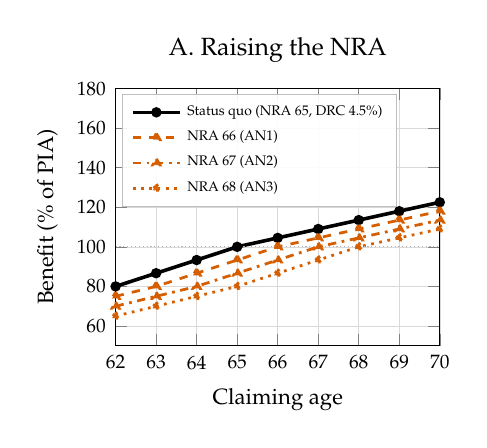
\begin{tikzpicture}
\begin{axis}[width=0.47\textwidth,height=0.40\textwidth,xmin=62,xmax=70,ymin=50,ymax=180,
  xtick={62,...,70},ytick={60,80,100,120,140,160,180},
  title={A. Raising the NRA},title style={font=\small},
  xlabel={Claiming age},ylabel={Benefit (\% of PIA)},
  grid=both,grid style={line width=.1pt, draw=gray!15},major grid style={line width=.2pt,draw=gray!30},
  tick label style={font=\scriptsize},label style={font=\footnotesize},
  legend style={font=\tiny,at={(0.02,0.98)},anchor=north west,draw=gray!50,fill=white,fill opacity=0.9,text opacity=1},legend cell align=left]
\addplot[black,line width=1.3pt,mark=*,mark size=1.2pt] coordinates {(62,80) (63,86.67) (64,93.33) (65,100) (66,104.5) (67,109) (68,113.5) (69,118) (70,122.5)};
\addlegendentry{Status quo (NRA 65, DRC 4.5\%)}
\addplot[red,line width=1pt,dashed,mark=triangle*,mark size=1.5pt] coordinates {(62,75) (63,80) (64,86.67) (65,93.33) (66,100) (67,104.5) (68,109) (69,113.5) (70,118)};
\addlegendentry{NRA 66 (AN1)}
\addplot[red,line width=1pt,dashdotted,mark=triangle*,mark size=1.5pt] coordinates {(62,70) (63,75) (64,80) (65,86.67) (66,93.33) (67,100) (68,104.5) (69,109) (70,113.5)};
\addlegendentry{NRA 67 (AN2)}
\addplot[red,line width=1pt,dotted,mark=triangle*,mark size=1.5pt] coordinates {(62,65) (63,70) (64,75) (65,80) (66,86.67) (67,93.33) (68,100) (69,104.5) (70,109)};
\addlegendentry{NRA 68 (AN3)}
\draw[gray!60,densely dotted] (axis cs:62,100) -- (axis cs:70,100);
\end{axis}
\end{tikzpicture}
 & % Generated by gen_figs.py from FROT tables/DRC_visualization_4.tex (program rules: benefit as % of PIA by claiming age).
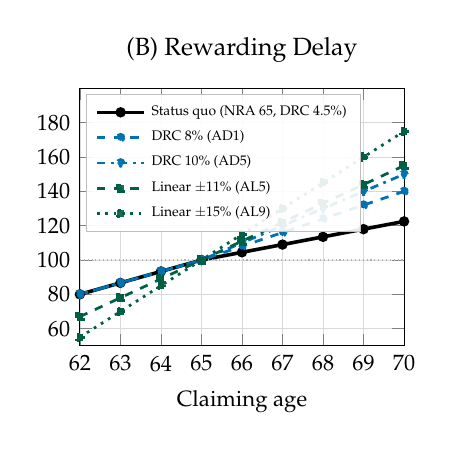
\begin{tikzpicture}
\begin{axis}[width=0.47\textwidth,height=0.40\textwidth,xmin=62,xmax=70,ymin=50,ymax=200,
  xtick={62,...,70},ytick={60,80,100,120,140,160,180},
  title={(B) Rewarding Delay},title style={font=\small},
  xlabel={Claiming age},
  grid=both,grid style={line width=.1pt, draw=gray!15},major grid style={line width=.2pt,draw=gray!30},
  tick label style={font=\footnotesize},label style={font=\footnotesize},
  legend style={font=\tiny,at={(0.02,0.98)},anchor=north west,draw=gray!50,fill=white,fill opacity=0.9,text opacity=1},legend cell align=left]
\addplot[black,line width=1.3pt,mark=*,mark size=1.2pt] coordinates {(62,80) (63,86.67) (64,93.33) (65,100) (66,104.5) (67,109) (68,113.5) (69,118) (70,122.5)};
\addlegendentry{Status quo (NRA 65, DRC 4.5\%)}
\addplot[blue,line width=1pt,dashed,mark=*,mark size=1.2pt] coordinates {(62,80) (63,86.67) (64,93.33) (65,100) (66,108) (67,116) (68,124) (69,132) (70,140)};
\addlegendentry{DRC 8\% (AD1)}
\addplot[blue,line width=1pt,dashdotted,mark=*,mark size=1.2pt] coordinates {(62,80) (63,86.67) (64,93.33) (65,100) (66,110) (67,120) (68,130) (69,140) (70,150)};
\addlegendentry{DRC 10\% (AD5)}
\addplot[green!60!black,line width=1pt,dashed,mark=square*,mark size=1.2pt] coordinates {(62,67) (63,78) (64,89) (65,100) (66,111) (67,122) (68,133) (69,144) (70,155)};
\addlegendentry{Linear $\pm$11\% (AL5)}
\addplot[green!60!black,line width=1pt,dotted,mark=square*,mark size=1.2pt] coordinates {(62,55) (63,70) (64,85) (65,100) (66,115) (67,130) (68,145) (69,160) (70,175)};
\addlegendentry{Linear $\pm$15\% (AL9)}
\draw[gray!60,densely dotted] (axis cs:62,100) -- (axis cs:70,100);
\end{axis}
\end{tikzpicture}

\end{tabular}
\tabnotes{\textit{Notes:} Retirement benefit received by an individual who claims at each age from 62 to 70, in percent of the primary insurance amount (PIA). Status quo (black): normal retirement age (NRA) of 65, reduction of 6.67 percent of the PIA per year of claiming before the NRA, and delayed retirement credit (DRC) of 4.5 percent of the PIA per year of claiming after the NRA, the rules of the 1920--1940 birth cohorts. Panel A: AN1--AN3 raise the NRA to 66, 67, and 68. Panel B: AD1 and AD5 raise the DRC to 8 and 10 percent; AL5 and AL9 set both the early-claiming reduction and the DRC to 11 and 15 percent per year. \autoref{tab:schedules} reports the schedules of all reforms; Appendix~\ref{app:reforms} describes their construction.}
\end{figure}

\autoref{tab:claiming} reports the results. Raising the NRA lowers welfare and saves money. An NRA of 66, 67, or 68 lowers WTP by 0.38, 0.74, or 1.09 percent and lowers net government spending by 0.87, 1.75, or 2.38 percent. The saving comes from Social Security itself: retirement outlays fall by 6.13, 11.82, and 16.75 percent, whereas the indirect effects are small, between $-0.02$ and $-0.12$ percent. The taxes paid by individuals who work longer are partly offset elsewhere in the budget: participation falls slightly at ages 30--49 and, for the two larger increases, at 62--64, and DI, which is paid until the NRA, is paid for longer to individuals with a disability, so that part of the saving on retirement benefits reappears as DI outlays (Section~\ref{sec:model_di}). Participation rises at 65--69, by 0.60, 1.98, and 3.27 points. This is an income effect: with lower benefits at every claiming age, individuals work longer to finance their retirement. The small decline at 30--49 reflects the lower return to the earnings that build the AIME when each dollar of PIA pays less.

\begin{table}[!htbp]
\centering
\caption{Reforms of the Claiming-Age Schedule}\label{tab:claiming}
\footnotesize
\setlength{\tabcolsep}{4.5pt}
% Source: FROT tables/welfare_age_dependence_mvpfv5.tex (May 2025 simulation of the estimated model). Authors: rerun on corrected code before submission if results changed.
% Generated by gen_tables.py from FROT tables/welfare_age_dependence_mvpfv5.tex.
% Source numbers: May 2025 simulation of the estimated model (FROT 2025 submission). Do not edit numbers by hand.
\begin{tabular}{@{}l l c c c c c c c c@{}}
\toprule
 & & \multicolumn{2}{c}{Welfare} & \multicolumn{3}{c}{Fiscal cost (\% change)} & \multicolumn{3}{c}{$\Delta$ Participation (pp)} \\
\cmidrule(lr){3-4}\cmidrule(lr){5-7}\cmidrule(lr){8-10}
 & Reform & MVPF & WTP (\%) & Net & Direct & Indirect & 30--49 & 62--64 & 65--69 \\
\midrule
\multicolumn{10}{@{}l}{\textit{A. Raising the normal retirement age (NRA)}} \\
(AN1) & NRA at 66 & 0.17 & $-$0.38 & $-$0.87 & $-$6.13 & $-$0.02 & $-$0.04 & 0.38 & 0.60 \\
(AN2) & NRA at 67 & 0.16 & $-$0.74 & $-$1.75 & $-$11.82 & $-$0.12 & $-$0.07 & $-$0.04 & 1.98 \\
(AN3) & NRA at 68 & 0.18 & $-$1.09 & $-$2.38 & $-$16.75 & $-$0.08 & $-$0.14 & $-$0.43 & 3.27 \\
\addlinespace
\multicolumn{10}{@{}l}{\textit{B. Raising the delayed retirement credit (DRC)}} \\
(AD1) & DRC at 8\% & $\infty$ & 0.16 & $-$0.45 & $-$2.46 & $-$0.10 & 0.11 & 0.15 & 0.74 \\
(AD2) & DRC at 8.5\% & $\infty$ & 0.19 & $-$0.44 & $-$2.87 & $-$0.04 & 0.10 & 0.18 & 0.57 \\
(AD3) & DRC at 9\% & $\infty$ & 0.23 & $-$0.66 & $-$4.22 & $-$0.07 & 0.09 & $-$0.36 & 1.20 \\
(AD4) & DRC at 9.5\% & $\infty$ & 0.26 & $-$0.73 & $-$4.56 & $-$0.09 & 0.12 & $-$0.49 & 1.37 \\
(AD5) & DRC at 10\% & $\infty$ & 0.3 & $-$0.78 & $-$5.05 & $-$0.08 & 0.14 & $-$0.97 & 1.39 \\
\addlinespace
\multicolumn{10}{@{}l}{\textit{C. Symmetric actuarial adjustment around the NRA}} \\
(AL1) & Linear $\pm$7\% & $\infty$ & 0.10 & $-$0.12 & $-$0.74 & $-$0.01 & 0.05 & 0.24 & 0.22 \\
(AL2) & Linear $\pm$8\% & $\infty$ & 0.15 & $-$0.46 & $-$2.81 & $-$0.07 & 0.11 & 0.05 & 0.61 \\
(AL3) & Linear $\pm$9\% & $\infty$ & 0.21 & $-$0.72 & $-$4.74 & $-$0.07 & 0.11 & $-$0.31 & 1.21 \\
(AL4) & Linear $\pm$10\% & $\infty$ & 0.29 & $-$0.86 & $-$5.54 & $-$0.09 & 0.14 & $-$0.93 & 1.42 \\
(AL5) & Linear $\pm$11\% & $\infty$ & 0.37 & $-$1.17 & $-$7.02 & $-$0.19 & 0.19 & $-$1.15 & 2.01 \\
(AL6) & Linear $\pm$12\% & $\infty$ & 0.47 & $-$1.37 & $-$7.72 & $-$0.28 & 0.30 & $-$1.46 & 2.61 \\
(AL7) & Linear $\pm$13\% & $\infty$ & 0.57 & $-$1.38 & $-$8.21 & $-$0.23 & 0.32 & $-$2.90 & 2.50 \\
(AL8) & Linear $\pm$14\% & $\infty$ & 0.69 & $-$1.47 & $-$8.22 & $-$0.31 & 0.34 & $-$3.30 & 2.42 \\
(AL9) & Linear $\pm$15\% & $\infty$ & 0.80 & $-$1.57 & $-$8.45 & $-$0.37 & 0.36 & $-$3.49 & 2.26 \\
\bottomrule
\end{tabular}

\tabnotes{\textit{Notes:} Each row reports the outcomes of simulating the estimated model for the 1920--1940 birth cohorts under the reform, announced before age 30 and in force over the life cycle, with prices held fixed (partial equilibrium). Status quo: NRA of 65, early-claiming reduction of 6.67 percent of the PIA per year, DRC of 4.5 percent per year. AN1--AN3 raise the NRA; AD1--AD5 raise the DRC in steps of 0.5 percentage points; AL1--AL9 set the early-claiming reduction and the DRC to a common rate of 7 to 15 percent per year (\autoref{fig:schedules} and \autoref{tab:schedules}). WTP: ex ante consumption-equivalent welfare change at age 30, in percent of consumption at every age. Direct: percentage change in the present value of Social Security retirement benefits, including the effect of claiming responses. Indirect: percentage change in the present value of all other taxes and transfers (DI benefits and consumption-floor transfers, net of income- and payroll-tax revenue). Net: percentage change in the present value of government spending. Present values are per capita and discounted to age 62 at the net interest rate (Section~\ref{sec:fw_fiscal}); because the three fiscal columns have different bases, Net is not the sum of Direct and Indirect. MVPF: WTP valued with the present value of per capita baseline consumption from age 62, divided by the dollar change in the present value of per capita government spending (equation~\eqref{eq:mvpf}). $\infty$: WTP $>0$ and net cost $<0$; here the direct cost is also negative, so the lower bound of equation~\eqref{eq:mvpf_lb} is infinite as well. For AN1--AN3, which lower welfare and save money, the MVPF is the welfare cost per dollar saved. $\Delta$ Participation: change in the labor force participation rate at ages 30--49, 62--64, and 65--69, in percentage points.}
\end{table}

The MVPFs of the NRA increases, 0.17, 0.16, and 0.18, are welfare costs per dollar saved: each dollar of government spending saved by raising the NRA costs the cohort 16 to 18 cents of willingness to pay, in dollars of consumption from age 62. Up to the baseline used for the dollar conversion, they are also the MVPFs of the reverse reforms, which would return the NRA to 65 for a cohort that faces a higher NRA: the shadow price of raising revenue by cutting the policy \citep{hendren2020unified}. The MVPF is nearly constant across the three increases.

Reforms that reward delay raise welfare and save money. Every AD and AL reform has a positive WTP, from 0.10 percent for AL1 to 0.80 percent for AL9, and lowers net, direct, and indirect spending. Their MVPF is therefore infinite under any accounting: with the net cost, with the direct cost alone (equation~\eqref{eq:mvpf_lb}), or with any partial count of the fiscal externalities.

The direct effect is the most informative column. Because an AD reform raises the benefit at every claiming age above the NRA and lowers none, its mechanical effect on retirement outlays, evaluated at unchanged claiming ages, is nonnegative. Yet retirement outlays fall, by 2.46 percent under AD1 and by 5.05 percent under AD5. The claiming responses induced by the higher credit therefore more than pay for the higher credit within Social Security, before any effect on taxes. Section~\ref{sec:fw_claiming} gives the accounting. A one-year delay lowers the present value of a claimant's benefits when the credit is below the rate that makes the delay actuarially fair for that claimant from the government's perspective (equation~\eqref{eq:faircredit}), and this rate is higher for claimants with lower survival. The fall in direct outlays implies that, at credits of 8 to 10 percent, the delays the reforms induce occur mostly among claimants for whom the new credit is still below their actuarially fair rate.\footnote{Two features of the model bear on the level of the fair rate. The horizon ends at age 85, which truncates the stream of benefits that a delay raises and therefore raises the fair rate relative to an economy with survival beyond 85. Benefits are discounted at the net return $r$; a lower discount rate for the government would lower the fair rate.} In terms of the decomposition of Section~\ref{sec:fw_decomp}, the behavioral fiscal externality of an AD reform is negative and larger in absolute value than its mechanical cost, so the ratio of the net to the mechanical cost is negative. The indirect effects add to the saving: longer careers raise income- and payroll-tax revenue, and the net cost of all other programs falls by 0.01 to 0.37 percent across the AD and AL reforms.

The moderate reforms raise participation in every age group we track. AD1, AD2, AL1, and AL2 raise participation by 0.05 to 0.11 points at 30--49, by 0.05 to 0.24 points at 62--64, and by 0.22 to 0.74 points at 65--69. The response at young ages reflects the higher value of a dollar of PIA for those who expect to claim late. Steeper schedules move participation at 62--64 and at 65--69 in opposite directions. From AD3 and AL3 on, participation at 62--64 falls, by up to 3.49 points under AL9, while participation at 65--69 rises by 1.20 to 2.61 points. We interpret this pattern as selection by health. A steeper schedule widens the gap between the benefits of early and late claimers and sorts individuals more sharply by the cost of continued work: those in good health, with low costs of work, stay longer to collect the larger credit, while less healthy workers leave earlier. The larger credit is also a windfall, at unchanged behavior, for those who would claim late in any case, and its income effect lowers their participation before 65. The fiscal saving nonetheless grows with the slope of the schedule: from AL3 to AL9, the indirect saving rises from 0.07 to 0.37 percent even as participation at 62--64 falls.

The contrast between the two families comes from the difference between a reward and a mandate when the cost of work differs across individuals. A credit is paid only to those who choose to delay. By revealed preference, they are the individuals for whom continued work is least costly relative to its reward: those in good health, with low fixed costs of work, and with higher wages. The credit leaves unchanged the option to claim early for those whose health makes work costly, and under the AD reforms it leaves their benefits unchanged as well. Because WTP is computed at age 30, before health is known, this preserved option is valued as insurance against bad health. An NRA increase is a benefit cut for everyone. It saves money mechanically, and the participation it generates at 65--69 is the income effect of being poorer rather than a response to a higher reward. Its cost falls also on those who cannot delay cheaply: individuals in poor health, who face a higher fixed cost of work (Section~\ref{sec:estimation}), claim early, and receive less whenever they claim.

The symmetric reforms combine a larger credit with a larger reduction for early claiming, and comparing reforms with the same credit isolates the role of the reduction. AL2 and AD1 both pay a credit of 8 percent; AL4 and AD5 both pay 10 percent. The additional reduction for early claiming adds little to the saving ($-0.46$ against $-0.45$ percent; $-0.86$ against $-0.78$ percent) and subtracts little from WTP (0.15 against 0.16 percent; 0.29 against 0.30 percent). The reward does most of the work. The steepest AL reforms raise welfare by more than any AD reform because their credits, 11 to 15 percent, are larger. Within the AL family, WTP and fiscal savings both rise with the slope of the schedule up to the steepest reform we consider, so our grid does not reach the slope at which further steepening would stop paying for itself. This is in line with the finding of \citet{NdiayeYu2026frot} that, in the constrained-efficient allocation of the same economy, consumption in retirement rises with the claiming age more steeply than the statutory credit implies.

Two reforms in our grid reproduce, for the cohort we study, the two changes to claiming incentives in the Social Security Amendments of 1983, which raised the NRA from 65 to 67 and the DRC to 8 percent per year, both phased in by birth cohort \citep{Svahn1983social}. AN2 sets the NRA at 67, and AD1 sets the DRC at 8 percent. In the model, the credit increase raises welfare by 0.16 percent and lowers government spending by 0.45 percent, an infinite MVPF; the NRA increase lowers welfare by 0.74 percent and saves 1.75 percent, an MVPF of 0.16. The two halves of the change in claiming incentives sit at opposite ends of the ranking. This is a comparison within the model, for cohorts born between 1920 and 1940. It is not an evaluation of the 1983 law, which changed other provisions as well and applied to later cohorts (Section~\ref{sec:discussion}).

In our grid, rewarding delay dominates mandating it for moderate fiscal savings. AD5 saves 0.78 percent of government spending, against 0.87 percent for AN1, and raises welfare by 0.30 percent where AN1 lowers it by 0.38 percent. AL4 saves 0.86 percent and raises welfare by 0.29 percent. AL9 saves more than AN1, 1.57 percent, raises welfare by 0.80 percent, and raises participation at 65--69 by more, 2.26 against 0.60 points. Only the two larger NRA increases save more than any reward-delay reform in the grid, 1.75 and 2.38 percent; Section~\ref{sec:financing} draws the implications for closing a financing gap. In the model, the NRA affects behavior only through the benefit schedule; Section~\ref{sec:discussion} discusses evidence that statutory ages also act as reference points \citep{seibold2021reference}.

% ---------------------------------------------------------------------------
\subsection{Benefit Progressivity and Level}\label{sec:results_generosity}

The second family changes the benefit formula itself. P1.1--P1.9 raise the replacement rate of the first bracket of the PIA formula from 0.90 to between 0.91 and 0.99. The level reforms L0--L9 raise all three rates proportionally, by 1 to 10 percent. \autoref{tab:generosity_app} in Appendix~\ref{app:figures} reports reforms that raise the second rate (P2) and then the third rate (P3), in each case on top of a first rate of 0.99. At unchanged behavior, each of these reforms raises the benefit of every retiree with a given AIME, so its mechanical effect is a transfer to retirees. All of them raise Social Security outlays, and all but the smallest raise net government spending (\autoref{tab:generosity}).

\begin{table}[!htbp]
\centering
\caption{Reforms of Benefit Progressivity and Level}\label{tab:generosity}
\footnotesize
\setlength{\tabcolsep}{4.5pt}
% Source: FROT tables/welfare_progressivity_mvpfv7.tex, rows P1 and L (May 2025 simulation of the estimated model). Authors: rerun on corrected code before submission if results changed.
% Generated by gen_tables.py from FROT tables/welfare_progressivity_mvpfv7.tex (rows P1, L).
% Source numbers: May 2025 simulation of the estimated model (FROT 2025 submission). Do not edit numbers by hand.
\begin{tabular}{@{}l l c c c c c c c c@{}}
\toprule
 & & \multicolumn{2}{c}{Welfare} & \multicolumn{3}{c}{Fiscal cost (\% change)} & \multicolumn{3}{c}{$\Delta$ Participation (pp)} \\
\cmidrule(lr){3-4}\cmidrule(lr){5-7}\cmidrule(lr){8-10}
 & PIA rates & MVPF & WTP (\%) & Net & Direct & Indirect & 30--49 & 62--64 & 65--69 \\
\midrule
\multicolumn{10}{@{}l}{\textit{A. Raising the first PIA rate (bottom bracket)}} \\
(P1.1) & (0.91, 0.32, 0.15) & $[0.52,\, +\infty)$ & 0.10 & $-$0.03 & 0.57 & $-$0.10 & 0.08 & 0.20 & 0.06 \\
(P1.2) & (0.92, 0.32, 0.15) & 0.97 & 0.22 & 0.09 & 1.23 & $-$0.07 & 0.14 & $-$0.07 & 0.00 \\
(P1.3) & (0.93, 0.32, 0.15) & 0.92 & 0.31 & 0.13 & 1.66 & $-$0.09 & 0.14 & 0.15 & 0.01 \\
(P1.4) & (0.94, 0.32, 0.15) & 0.84 & 0.40 & 0.19 & 2.16 & $-$0.10 & 0.14 & $-$0.17 & $-$0.23 \\
(P1.5) & (0.95, 0.32, 0.15) & 0.91 & 0.50 & 0.21 & 2.32 & $-$0.09 & 0.16 & $-$0.34 & $-$0.31 \\
(P1.6) & (0.96, 0.32, 0.15) & 1.14 & 0.59 & 0.20 & 2.80 & $-$0.16 & 0.19 & $-$0.27 & $-$0.15 \\
(P1.7) & (0.97, 0.32, 0.15) & 1.01 & 0.67 & 0.26 & 3.22 & $-$0.16 & 0.21 & $-$0.57 & $-$0.50 \\
(P1.8) & (0.98, 0.32, 0.15) & 0.86 & 0.75 & 0.34 & 3.72 & $-$0.15 & 0.24 & $-$0.71 & $-$0.49 \\
(P1.9) & (0.99, 0.32, 0.15) & 0.69 & 0.80 & 0.44 & 4.12 & $-$0.11 & 0.25 & $-$0.85 & $-$0.60 \\
\addlinespace
\multicolumn{10}{@{}l}{\textit{B. Raising all PIA rates proportionally (level)}} \\
(L0) & (0.909, 0.3232, 0.1515) & 0.51 & 0.16 & 0.12 & 1.34 & $-$0.05 & 0.11 & $-$0.05 & 0.01 \\
(L1) & (0.918, 0.3264, 0.153) & 0.59 & 0.32 & 0.21 & 2.47 & $-$0.11 & 0.14 & $-$0.15 & $-$0.13 \\
(L2) & (0.927, 0.3296, 0.1545) & 0.49 & 0.46 & 0.36 & 3.48 & $-$0.10 & 0.13 & $-$0.49 & $-$0.08 \\
(L3) & (0.936, 0.3328, 0.156) & 0.61 & 0.60 & 0.38 & 4.25 & $-$0.18 & 0.18 & $-$0.29 & $-$0.3 \\
(L4) & (0.945, 0.336, 0.1575) & 0.59 & 0.74 & 0.49 & 5.28 & $-$0.21 & 0.21 & $-$0.48 & $-$0.43 \\
(L5) & (0.954, 0.3392, 0.159) & 0.52 & 0.87 & 0.64 & 6.31 & $-$0.19 & 0.23 & $-$0.72 & $-$0.68 \\
(L6) & (0.963, 0.3424, 0.1605) & 0.47 & 0.95 & 0.79 & 7.41 & $-$0.20 & 0.24 & $-$1.00 & $-$1.22 \\
(L7) & (0.972, 0.3456, 0.162) & 0.42 & 1.00 & 0.92 & 8.66 & $-$0.23 & 0.26 & $-$1.40 & $-$1.43 \\
(L8) & (0.981, 0.3488, 0.1635) & 0.35 & 1.02 & 1.14 & 9.80 & $-$0.18 & 0.27 & $-$1.76 & $-$1.86 \\
(L9) & (0.99, 0.352, 0.165) & 0.30 & 0.98 & 1.24 & 10.70 & $-$0.20 & 0.28 & $-$2.37 & $-$1.99 \\
\bottomrule
\end{tabular}

\tabnotes{\textit{Notes:} Each row reports the outcomes of simulating the estimated model for the cohort under the reform, announced before age 30 and in force over the life cycle, with prices held fixed (partial equilibrium). The second column gives the three replacement rates of the PIA formula (first, second, and third bracket of the AIME); the status quo is (0.90, 0.32, 0.15). P1.1--P1.9 raise the first rate by 1 to 9 percentage points; L0--L9 raise all three rates proportionally by 1 to 10 percent. L9 sets the same rates as P3.9 in \autoref{tab:generosity_app}. WTP: ex ante consumption-equivalent welfare change at age 30, in percent. Direct: percentage change in the present value of Social Security retirement benefits. Indirect: percentage change in the present value of all other taxes and transfers (DI benefits and consumption-floor transfers, net of income- and payroll-tax revenue). Net: percentage change in the present value of government spending. Present values are per capita and discounted to age 62 (Section~\ref{sec:fw_fiscal}). MVPF: WTP valued with the present value of per capita baseline consumption from age 62, divided by the dollar change in government spending (equation~\eqref{eq:mvpf}). For P1.1, the net cost is negative and the MVPF infinite; the interval reports as lower bound the MVPF computed with the direct cost only (equation~\eqref{eq:mvpf_lb}). $\Delta$ Participation: change in the labor force participation rate at the indicated ages, in percentage points.}
\end{table}

The smallest expansion of the bottom bracket, P1.1, is the exception. It raises retirement outlays by 0.57 percent but lowers net government spending by 0.03 percent, so its MVPF is infinite; counting only its direct cost gives a lower bound of 0.52. The saving comes from participation: P1.1 raises participation in all three age groups, and the income taxes paid by the additional participants account for 57 percent of its indirect fiscal effect. % Source: FROT 2025_sub/7_policy_reforms.tex (Social Security Progressivity and Level Reforms)
The larger expansions of the first rate, P1.2--P1.9, have MVPFs between 0.69 and 1.14, the lowest for the largest reform. The level reforms have MVPFs between 0.30 and 0.61. Raising the second rate lowers the MVPF from 0.56 to 0.29, and raising the third rate leaves it at 0.29--0.30.

The generosity reforms move participation in opposite directions over the life cycle. At ages 30--49 participation rises slightly, by 0.08 to 0.28 points across all P and L reforms: because benefits depend on the AIME, a higher replacement rate raises the return to the earnings that build it. At older ages, the larger reforms lower participation through an income effect; under L9, participation falls by 2.37 points at 62--64 and by 1.99 points at 65--69. The indirect effects are small and negative for every reform: on net, the taxes gained from more work at 30--49 and the lower consumption-floor transfers to retirees with higher benefits outweigh the taxes lost from less work at older ages and the higher DI benefits that follow from a higher PIA.

The bottom bracket delivers the most welfare per dollar because of whom it pays. Comparing reforms with similar costs isolates this. P1.6 and L1 have net costs of 0.20 and 0.21 percent, but WTP of 0.59 and 0.32 percent and MVPFs of 1.14 and 0.59. P1.9 and L3 have similar direct costs (4.12 and 4.25 percent) and net costs (0.44 and 0.38 percent), but WTP of 0.80 and 0.60 percent. The difference lies in welfare, not in fiscal externalities. A dollar spent on the first bracket goes to retirees with a low AIME. In the model, a low AIME is the cumulative result of low ability and of health shocks that lowered wages, raised the cost of work, and shortened careers; retirees with such histories have few assets and a high marginal utility of consumption. Because WTP is measured before these histories are realized, a transfer toward them is insurance. A level increase spreads the same dollar over all retirees, including those with high lifetime earnings. Raising the upper rates on top of a first rate of 0.99 adds little welfare: from P1.9 to P2.9, WTP rises from 0.80 to 0.95 percent while the net cost rises from 0.44 to 1.27 percent, and the P3 reforms leave both nearly unchanged (\autoref{tab:generosity_app}).

This result bears on a lesson from dynamic taxation. In models in which retirement is exogenous, linear, age-dependent taxes that do not depend on earnings histories come close to the optimum \citep{farhi2013insurance}. In our economy, Social Security, whose benefits depend on the whole earnings history through the AIME, is the most valuable instrument (Section~\ref{sec:results_elim}), and the value of an additional dollar of benefits is highest where the formula targets low lifetime earnings. The history dependence of benefits is where the value lies.

% ---------------------------------------------------------------------------
\subsection{Medicare}\label{sec:results_medicare}

Panel A of \autoref{tab:other} reports two expansions of Medicare. For these reforms, the baseline coverage rates of medical expenditures after age 65 are re-estimated from the MEPS by health and working status, and the model with these rates serves as the status quo (Appendix~\ref{app:reforms}). The Part A reform raises the coverage rate of all individuals aged 65 and over by 20 percentage points; the Part B reform raises it by 20 points for nonparticipants only.\footnote{Part A covers mainly inpatient services and is premium-free for most beneficiaries. Part B covers physician and outpatient services, which most employer-provided plans also cover, and requires a premium; we therefore target the Part B expansion at nonparticipants.} % Source: FROT 2025_sub/7_policy_reforms.tex (Medicare Reforms)

\begin{table}[!htbp]
\centering
\caption{Reforms of Medicare, Old-Age Income Taxes, and Savings Returns}\label{tab:other}
\footnotesize
\setlength{\tabcolsep}{4.5pt}
% Source: FROT tables/welfare_medicare_mvpfv8.tex, welfare_tax_mvpf_v8.tex, welfare_savings_mvpf_v3.tex (May 2025 simulation of the estimated model). Authors: rerun on corrected code before submission if results changed.
% Generated by gen_tables.py from FROT tables/welfare_medicare_mvpfv8.tex, welfare_tax_mvpf_v8.tex, welfare_savings_mvpf_v3.tex.
% Source numbers: May 2025 simulation of the estimated model (FROT 2025 submission). Do not edit numbers by hand.
\begin{tabular}{@{}l l c c c c c c c c@{}}
\toprule
 & & \multicolumn{2}{c}{Welfare} & \multicolumn{3}{c}{Fiscal cost (\% change)} & \multicolumn{3}{c}{$\Delta$ Participation (pp)} \\
\cmidrule(lr){3-4}\cmidrule(lr){5-7}\cmidrule(lr){8-10}
 & Reform & MVPF & WTP (\%) & Net & Direct & Indirect & 30--49 & 62--64 & 65--69 \\
\midrule
\multicolumn{10}{@{}l}{\textit{A. Medicare: coverage of medical expenditures after age 65 raised by 20 percentage points}} \\
(MA) & Part A: all individuals & 0.146 & 1.36 & 3.53 & 45.17 & 0.10 & 0.22 & $-$1.70 & $-$0.38 \\
(MB) & Part B: nonparticipants & 0.155 & 1.30 & 3.19 & 41.61 & 0.03 & 0.21 & $-$1.95 & $-$3.44 \\
\addlinespace
\multicolumn{10}{@{}l}{\textit{B. Old-age income tax: after-tax income at ages 62+ raised by $x$ percent per year of age above 61}} \\
(I1) & $x=1\%$ & 0.25 & 0.44 & 0.69 & 0.70 & $-$0.81 & 0.06 & 0.76 & 1.98 \\
(I2) & $x=2\%$ & 0.26 & 0.87 & 1.28 & 1.31 & $-$1.51 & 0.15 & 1.58 & 4.12 \\
(I3) & $x=3\%$ & 0.25 & 1.29 & 2.01 & 2.03 & $-$2.18 & 0.18 & 2.76 & 6.07 \\
(I4) & $x=4\%$ & 0.23 & 1.69 & 2.80 & 2.80 & $-$2.78 & 0.2 & 3.19 & 7.71 \\
(I5) & $x=5\%$ & 0.23 & 2.09 & 3.46 & 3.47 & $-$3.58 & 0.26 & 4.11 & 8.92 \\
\addlinespace
\multicolumn{10}{@{}l}{\textit{C. Savings subsidy: net return on assets raised at all ages}} \\
(K1) & +0.2 pp & $[0.96,\,20.37]$ & 0.87 & 0.08 & 1.77 & $-$1.69 & 0.15 & $-$1.27 & $-$0.85 \\
(K2) & +0.4 pp & $[0.92,\,19.38]$ & 1.75 & 0.18 & 3.77 & $-$3.59 & 0.36 & $-$2.58 & $-$1.75 \\
(K3) & +0.8 pp & $[0.84,\,5.29]$ & 3.6 & 1.34 & 8.44 & $-$7.10 & 0.38 & $-$5.98 & $-$4.11 \\
\bottomrule
\end{tabular}

\tabnotes{\textit{Notes:} Each row reports the outcomes of simulating the estimated model for the cohort under the reform, announced before age 30 and in force over the life cycle, with prices held fixed (partial equilibrium). WTP: ex ante consumption-equivalent welfare change at age 30, in percent. Fiscal columns (Section~\ref{sec:fw_fiscal}; present values per capita, discounted to age 62): \textit{Panel A.} Coverage rates after 65 by health and working status re-estimated from the MEPS form the baseline; MA raises coverage of all individuals aged 65 and over, MB coverage of nonparticipants aged 65 and over. Direct: change in the present value of Medicare's payments to the targeted beneficiaries, in percent of baseline payroll-tax revenue. Indirect: percentage change in the present value of all taxes and transfers, including Social Security benefits. Net: change in government spending plus Medicare's payments to the targeted beneficiaries, in percent of baseline government spending. \textit{Panel B.} I1--I5 replace the level parameter $\lambda_t$ of the after-tax income schedule $\lambda_t y^{1-\tau_t}$ at ages $t\geq62$ by $\lambda_t+x(t-61)$, with $x$ from 0.01 to 0.05 (Appendix~\ref{app:reforms}). Direct: income-tax revenue forgone, in percent of its baseline present value. Indirect: percentage change in the present value of all other taxes and transfers, including Social Security benefits, net of payroll-tax revenue. Net: percentage change in government spending. \textit{Panel C.} K1--K3 raise the net return on assets at all ages; K3 sets it equal to the pretax return, as in D3 of \autoref{tab:elim}. Direct: present value of the subsidy, in percent of baseline government spending. Indirect: percentage change in government spending excluding the subsidy. Net: percentage change in government spending including the subsidy. MVPF (equation~\eqref{eq:mvpf}): WTP valued with the present value of per capita baseline consumption from age 62 in Panels A and B and from age 30 in Panel C, divided by the dollar change in government spending. In Panel C, the interval reports as lower bound the MVPF with the subsidy as the only cost (equation~\eqref{eq:mvpf_lb}) and as upper bound the MVPF with the net cost, which treats capital income as realized and taxed every period and therefore overstates the indirect saving. Because of the different consumption base, the levels of the MVPFs in Panel C are not comparable with those in Panels A and B (Section~\ref{sec:discussion}). $\Delta$ Participation: change in the labor force participation rate at the indicated ages, in percentage points.}
\end{table}

Both expansions raise welfare substantially, by 1.36 and 1.30 percent, but at a high cost. Medicare's payments to the targeted beneficiaries rise by an amount equal to 45.17 percent of baseline payroll-tax revenue for Part A and 41.61 percent for Part B, and net government spending, including these payments, rises by 3.53 and 3.19 percent. The cost is driven by large medical expenditures after age 70. % Source: FROT 2025_sub/7_policy_reforms.tex (Medicare Reforms)
The MVPFs are 0.146 and 0.155, the lowest among the benefit expansions we study. Coverage after 65 lowers participation at older ages: by 1.70 and 0.38 points at 62--64 and 65--69 under Part A, and by 1.95 and 3.44 points under Part B. Better coverage reduces the need to work and save for medical expenses in old age. Under Part B, the additional coverage is also conditional on not working, so that a worker over 65 who keeps working forgoes it; the expansion acts as an implicit tax on work, which accounts for its much larger participation response at 65--69. Lower participation reduces tax revenue, and the indirect effects are positive, 0.10 and 0.03 percent.

Estimates of the MVPF of the introduction of Medicare, based on variation in preexisting insurance coverage, lie between 0.52 and 3.83 \citep{finkelstein2008did,hendren2020unified}. Our estimates for expansions of an established program lie below this range, as diminishing returns to coverage would imply.\footnote{Estimates for subsidized health insurance for low-income adults find a willingness to pay well below the cost of coverage \citep{finkelstein2019subsidizing}; they concern a different population and program and are not directly comparable to ours.} Our Medicare MVPFs are close to those of the NRA increases, 0.16 to 0.18. In this economy, a dollar spent on additional Medicare coverage after 65 buys about as much welfare as a dollar spent on keeping the NRA at 65.

% ---------------------------------------------------------------------------
\subsection{Old-Age Income Taxes}\label{sec:results_tax}

Panel B of \autoref{tab:other} reports cuts in income taxes after age 61. Reforms I1--I5 raise the level parameter $\lambda_t$ of the after-tax income schedule $\lambda_t y^{1-\tau_t}$ at ages $t\geq 62$ to $\lambda_t+x(t-61)$, with $x$ from 0.01 to 0.05, so that the cut grows with age. These reforms produce the largest increases in old-age participation of any reform we study. Participation rises by 0.76 to 4.11 points at 62--64 and by 1.98 to 8.92 points at 65--69. The cut raises the after-tax return to work at older ages, and the substitution effect dominates the income effect. Participation also rises slightly at 30--49, by 0.06 to 0.26 points.

Despite these responses, the tax cuts do not pay for themselves. The induced work raises payroll-tax revenue and lowers other outlays, and the net cost of all other programs, including Social Security, falls by 0.81 to 3.58 percent. The revenue loss dominates: net spending rises by 0.69 to 3.46 percent, and the MVPFs lie between 0.23 and 0.26. The welfare gain per dollar is small because of whom the cut pays. Under the tax function, a higher $\lambda_t$ raises after-tax income in proportion to $y^{1-\tau_t}$, so the cut accrues mostly to individuals with high incomes in old age---those who keep working, typically in good health, and those with large pension and interest income---whose marginal utility is low. Ex ante, it is a transfer toward good states rather than insurance against bad ones.

The comparison with the claiming-age reforms shows that a large participation response is neither necessary nor sufficient for a high MVPF. The larger tax cuts raise participation at 65--69 by far more than any reward-delay reform, by up to 8.92 points against at most 2.61 points, and cost money; AD1 raises it by 0.74 points and saves money. What matters is the fiscal saving that a reform recovers from the behavior it induces relative to the transfer it makes to individuals who would have behaved the same way without it. A credit for delay pays nothing to those who claim at or before the NRA; a tax cut on old-age income pays every individual with old-age income.

% ---------------------------------------------------------------------------
\subsection{Savings Subsidies}\label{sec:results_savings}

Panel C of \autoref{tab:other} reports reforms that raise the net return on saving at all ages by 0.2, 0.4, and 0.8 percentage points. K3 raises the net return to the pretax return $r_f$ and is therefore the full subsidy of experiment D3; its WTP of 3.6 percent equals the welfare gain in \autoref{tab:elim}. The subsidies raise welfare by 0.87 to 3.6 percent. Their direct cost, the present value of the subsidy, is 1.77 to 8.44 percent of baseline government spending, but most of it returns to the budget: higher saving raises taxable interest income, and government spending excluding the subsidy falls by 1.69 to 7.10 percent, which leaves net costs of 0.08 to 1.34 percent. This recovery is an upper bound, because the model taxes interest income every period, as if capital income were realized and taxed as it accrues. We therefore report each MVPF as an interval. The lower bound counts only the subsidy as a cost and lies between 0.84 and 0.96; the upper bound uses the net cost and lies between 5.29 and 20.37.

The subsidies have a strong income effect at older ages. Participation falls by 1.27 to 5.98 points at 62--64 and by 0.85 to 4.11 points at 65--69, as individuals accumulate more wealth and retire earlier, while it rises slightly at 30--49. A higher return makes saving a better substitute for continued work as a source of old-age income.

The MVPFs of the savings subsidies rest on a different consumption base from those of the other reforms. Because a subsidy changes returns from age 30, its WTP is converted into dollars with the present value of baseline consumption from age 30 rather than from age 62 (Section~\ref{sec:fw_mvpf}). The lifetime base is larger, so the levels of the savings MVPFs, including their lower bounds, are not comparable with those of the reforms that start at 62. Section~\ref{sec:discussion} compares the two on a common base.

% ---------------------------------------------------------------------------
\subsection{Synthesis: The MVPF Map}\label{sec:results_map}

\autoref{fig:mvpfmap} places every reform in the plane of net fiscal cost and WTP. Both axes are measured in the same units for every reform, so the slope of the ray from the origin to a reform, WTP divided by net cost, is proportional to its MVPF on a common consumption base. For the reforms that start at 62, the MVPF equals, up to rounding, this slope times a common factor (Section~\ref{sec:fw_mvpf}).

\begin{figure}[!htbp]
\centering
\caption{The MVPF Map: Welfare and Net Fiscal Cost of All Reforms}\label{fig:mvpfmap}
\vspace{0.5em}
% Generated from the reform tables (FROT 2025 simulation): figures/mvpf_map.tex.
% Legend moved below the axis so that no marker is hidden (layout only; applied after the file's own axis options).
\pgfplotsset{every axis post/.append style={legend columns=3,legend style={at={(0.5,-0.16)},anchor=north,/tikz/every even column/.append style={column sep=0.6em}}}}
% Generated by gen_figs.py from the reform tables (FROT 2025 simulation). Each point is one reform:
% x = net fiscal cost (% change in NPV of government spending), y = WTP (consumption-equivalent welfare change, %).
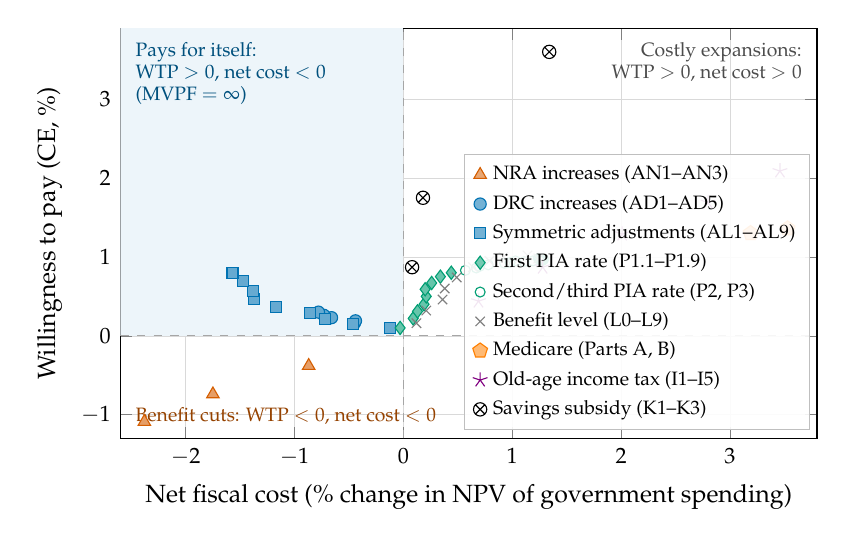
\begin{tikzpicture}
\begin{axis}[width=0.86\textwidth,height=0.56\textwidth,
  xmin=-2.6,xmax=3.8,ymin=-1.3,ymax=3.9,
  xlabel={Net fiscal cost (\% change in NPV of government spending)},
  ylabel={Willingness to pay (CE, \%)},
  grid=both,grid style={line width=.1pt, draw=gray!15},major grid style={line width=.2pt,draw=gray!30},
  tick label style={font=\footnotesize},label style={font=\small},
  legend style={font=\scriptsize,at={(0.99,0.02)},anchor=south east,draw=gray!50,fill=white,fill opacity=0.9,text opacity=1,cells={anchor=west}},
  legend cell align=left]
\fill[blue!7] (axis cs:-2.6,0) rectangle (axis cs:0,3.9);
\draw[gray!70,dashed] (axis cs:-2.6,0) -- (axis cs:3.8,0);
\draw[gray!70,dashed] (axis cs:0,-1.3) -- (axis cs:0,3.9);
\node[font=\scriptsize,align=left,anchor=north west,text=blue!70!black] at (axis cs:-2.55,3.85) {Pays for itself:\\ WTP $>0$, net cost $<0$\\ (MVPF $=\infty$)};
\node[font=\scriptsize,align=right,anchor=north east,text=black!70] at (axis cs:3.75,3.85) {Costly expansions:\\ WTP $>0$, net cost $>0$};
\node[font=\scriptsize,align=left,anchor=south west,text=red!70!black] at (axis cs:-2.55,-1.25) {Benefit cuts: WTP $<0$, net cost $<0$};
\addplot[only marks,mark=triangle*,mark size=2.6pt,color=red,mark options={solid,fill=red!60,draw=red}] coordinates {(-0.87,-0.38) (-1.75,-0.74) (-2.38,-1.09)};
\addlegendentry{NRA increases (AN1--AN3)}
\addplot[only marks,mark=*,mark size=2.2pt,color=blue,mark options={solid,fill=blue!60,draw=blue}] coordinates {(-0.45,0.16) (-0.44,0.19) (-0.66,0.23) (-0.73,0.26) (-0.78,0.3)};
\addlegendentry{DRC increases (AD1--AD5)}
\addplot[only marks,mark=square*,mark size=2.0pt,color=blue,mark options={solid,fill=blue!60,draw=blue}] coordinates {(-0.12,0.1) (-0.46,0.15) (-0.72,0.21) (-0.86,0.29) (-1.17,0.37) (-1.37,0.47) (-1.38,0.57) (-1.47,0.69) (-1.57,0.8)};
\addlegendentry{Symmetric adjustments (AL1--AL9)}
\addplot[only marks,mark=diamond*,mark size=2.4pt,color=green,mark options={solid,fill=green!60,draw=green}] coordinates {(-0.03,0.1) (0.09,0.22) (0.13,0.31) (0.19,0.4) (0.21,0.5) (0.2,0.59) (0.26,0.67) (0.34,0.75) (0.44,0.8)};
\addlegendentry{First PIA rate (P1.1--P1.9)}
\addplot[only marks,mark=o,mark size=1.8pt,color=green,mark options={solid,fill=green!60,draw=green}] coordinates {(0.57,0.83) (0.67,0.86) (0.7,0.88) (0.78,0.9) (0.93,0.92) (0.98,0.93) (1.03,0.95) (1.11,0.94) (1.19,0.95) (1.27,0.95) (1.26,0.95) (1.27,0.96) (1.28,0.96) (1.26,0.96) (1.27,0.96) (1.29,0.97) (1.27,0.97) (1.27,0.97) (1.25,0.97) (1.24,0.98)};
\addlegendentry{Second/third PIA rate (P2, P3)}
\addplot[only marks,mark=x,mark size=2.4pt,color=gray,mark options={solid,fill=gray!60,draw=gray}] coordinates {(0.12,0.16) (0.21,0.32) (0.36,0.46) (0.38,0.6) (0.49,0.74) (0.64,0.87) (0.79,0.95) (0.92,1) (1.14,1.02) (1.24,0.98)};
\addlegendentry{Benefit level (L0--L9)}
\addplot[only marks,mark=pentagon*,mark size=2.8pt,color=orange,mark options={solid,fill=orange!60,draw=orange}] coordinates {(3.53,1.36) (3.19,1.3)};
\addlegendentry{Medicare (Parts A, B)}
\addplot[only marks,mark=star,mark size=2.8pt,color=violet,mark options={solid,fill=violet!60,draw=violet}] coordinates {(0.69,0.44) (1.28,0.87) (2.01,1.29) (2.8,1.69) (3.46,2.09)};
\addlegendentry{Old-age income tax (I1--I5)}
\addplot[only marks,mark=otimes,mark size=2.4pt,color=black,mark options={solid,fill=black!60,draw=black}] coordinates {(0.08,0.87) (0.18,1.75) (1.34,3.6)};
\addlegendentry{Savings subsidy (K1--K3)}
\end{axis}
\end{tikzpicture}

\tabnotes{\textit{Notes:} Each marker is one reform of Tables~\ref{tab:claiming}, \ref{tab:generosity}, \ref{tab:generosity_app}, and~\ref{tab:other}. Horizontal axis: net fiscal cost, the percentage change in the present value of per capita government spending discounted to age 62 (Net). Vertical axis: willingness to pay, the ex ante consumption-equivalent welfare change at age 30, in percent (WTP). Shaded region: WTP $>0$ and net cost $<0$, where the MVPF is infinite. Lower-left quadrant: reforms that lower welfare and save money, for which the MVPF is the welfare cost per dollar saved. Upper-right quadrant: reforms that raise welfare at a positive net cost. For the reforms that start at age 62, the MVPF equals the slope of the ray from the origin times a common factor (Section~\ref{sec:fw_mvpf}). The savings subsidies use a different consumption base for their MVPFs, and their net costs treat capital income as taxed every period (\autoref{tab:other}). All entries come from simulations of the estimated model with prices held fixed.}
\end{figure}

The map has three regions. The shaded upper-left region contains the reforms that pay for themselves: all fourteen reforms that reward delay and the smallest expansion of the bottom bracket. Their savings are not small: the steepest symmetric reforms lie to the left of AN1. The lower-left quadrant contains the NRA increases, which lie on a flat ray: they save much per unit of welfare lost, but they lose welfare. The upper-right quadrant contains the costly expansions. Within it, the first-rate reforms lie above the level reforms at the same net cost; the reforms of the upper rates extend to the right at a nearly constant WTP, adding cost without adding welfare; the income-tax cuts lie along a ray of nearly constant slope, as their nearly constant MVPFs imply; and the Medicare expansions lie far to the right, on the flattest rays among the expansions.

Because the reforms that start at 62 share a common consumption base, their MVPFs can be ranked directly. Reforms that reward delay come first, with infinite MVPFs. Expansions of the bottom bracket follow, with MVPFs between 0.69 and 1.14 and an infinite MVPF for the smallest. Level reforms and increases in the upper rates follow at 0.29 to 0.61, then cuts in old-age income taxes at 0.23 to 0.26. A reduction of the NRA, the reverse of AN1--AN3, at 0.16 to 0.18, and the Medicare expansions, at 0.146 to 0.155, come last. The savings subsidies appear on the same axes, but their net costs rest on the upper-bound treatment of capital-income taxes, and Section~\ref{sec:discussion} places their MVPFs on the common base.

The ranking reflects two properties of a reform: whom it pays at unchanged behavior, and what it pays for at the margin. A credit for delay pays at the margin for delays that lower the program's outlays and pays nothing to those who cannot delay. The bottom bracket pays retirees whose lifetime earnings were depressed by low ability or poor health. A lower NRA pays every claimant, and an old-age tax cut pays in proportion to old-age income. A Medicare expansion pays for medical expenditures concentrated at the oldest ages, which drive its large cost.

\section{Closing a Financing Gap}\label{sec:financing}

Population aging puts the financing of Social Security under pressure \citep{trustees2024,cbo2024socialsecurity}, and closing a financing gap requires raising revenue or cutting outlays. The MVPF ranks the instruments available for this purpose by the welfare cost of each dollar they save \citep{hendren2016policy,hendren2020unified}. This section draws the implications of our estimates for that choice; all statements refer to the reforms in our grid and to the cohort we study.

\paragraph{Reforms that save money and raise welfare.} A reform with an infinite MVPF relaxes the budget at no welfare cost and therefore comes first in any consolidation. In our grid, these are the reforms that reward later claiming (\autoref{tab:claiming}). Their savings are not small. The DRC increases lower the present value of government spending by 0.44 to 0.78 percent, and the symmetric adjustments by 0.12 percent (AL1) to 1.57 percent (AL9), while raising welfare by 0.10 to 0.80 percent. Within the symmetric family, fiscal saving and welfare rise together with the slope of the schedule, so the reform that saves the most, AL9, also raises welfare the most. For these reforms there is no trade-off between the budget and welfare to resolve: the government obtains the saving by paying a larger reward to those who delay, and the induced delays and longer careers more than finance the reward (Section~\ref{sec:results_claiming}).

\paragraph{Rewarding delay and raising the NRA.} The relevant comparison is with increases in the NRA, the most common response to financing pressure. For a fiscal saving up to the size of AN1, 0.87 percent of government spending, several reward-delay reforms deliver a similar or larger saving with a welfare gain instead of a welfare loss. AD5 saves 0.78 percent and AL4 saves 0.86 percent; AL5, AL6, AL7, AL8, and AL9 save 1.17, 1.37, 1.38, 1.47, and 1.57 percent. AN1 lowers welfare by 0.38 percent; each of these reforms raises it. Larger consolidations are a different matter. AN2 and AN3 save 1.75 and 2.38 percent, more than any single reward-delay reform in our grid. We have not computed combinations of reforms, such as a steeper claiming schedule together with a higher NRA, so the grid does not say how a saving of that size would best be obtained. It does show that savings up to 1.57 percent of government spending can be obtained while raising welfare, and that, for the cohort we study, the steepest reward-delay reform saves more than an increase in the NRA from 65 to 66.

\paragraph{The welfare cost of a dollar saved.} Once the reforms with infinite MVPF are exhausted, further savings require reforms that lower welfare, and the MVPF of such a reform measures its welfare cost per dollar saved. Raising the NRA costs 16 to 18 cents of willingness to pay, in dollars of consumption from age 62, per dollar of government spending saved. Our grid contains two other families against which this cost can be compared, Medicare coverage after 65 and income taxes after 62, but we simulate them as expansions, with MVPFs of 0.146 to 0.155 and 0.23 to 0.26. To a first order, the MVPF of a cut equals the MVPF of the corresponding expansion. For a small change $d\theta$ in a policy parameter $\theta$, both the WTP and the net cost are proportional to $d\theta$; reversing the sign of $d\theta$ reverses the sign of both and leaves their ratio unchanged. Read this way, raising the NRA costs about as much welfare per dollar saved as forgoing or reversing an expansion of Medicare coverage after 65, and less than raising income taxes on older individuals, which would cost about 23 to 26 cents per dollar raised. Among the welfare-reducing instruments we consider, NRA increases are thus a comparatively inexpensive source of revenue, even though they are dominated by rewards for delay for moderate savings.

This symmetry is a first-order argument, and our reforms are not marginal. If the WTP is concave in the policy parameter, as diminishing returns imply, the welfare lost by moving the parameter down exceeds the welfare gained by moving it up by the same amount, and the reversed MVPFs understate the welfare cost of a cut. For old-age income taxes, the MVPFs of I1--I5 hardly change with the size of the reform, which suggests that this curvature is mild over the range we consider. For Medicare, the gap between our estimates and the estimates of the MVPF of its introduction, 0.52 to 3.83 (Section~\ref{sec:results_medicare}), suggests that the curvature is pronounced over larger changes, so that cuts in coverage could cost more per dollar than our expansions return. Behavioral responses to cuts and expansions also need not be symmetric when participation involves fixed costs of work and a cost of reentry. We have not simulated the reverse reforms, and the comparison between NRA increases and tax increases or Medicare cuts is an approximation rather than a computed result. The comparison between NRA increases and reward-delay reforms involves no such approximation.

\paragraph{Who bears the gap.} Our analysis concerns a single cohort, facing reforms announced before age 30 and in force over its whole life. A financing gap also raises the question of how a legacy debt is shared across cohorts, and a cohort analysis does not determine who should bear it. The MVPF ranks the instruments for raising a dollar from a given cohort; it does not say which cohorts should contribute that dollar. The transition generations, cohorts already in the middle of their careers or near retirement when a reform is announced, are not modeled. For them, both the welfare cost and the fiscal saving of a reform depend on how much of their working life remains when it is announced: an NRA increase announced late in a career leaves little room to adjust saving and labor supply, and a higher credit can change the behavior only of those who have not yet claimed. Prices are held fixed throughout, so the analysis also abstracts from the effects of a consolidation on wages and interest rates (Section~\ref{sec:discussion}).

With these qualifications, the MVPFs suggest an order for closing a financing gap. Reforms that reward later claiming come first, because they save money and raise welfare. Beyond the savings they can deliver, the choice among reforms that lower welfare should follow their welfare cost per dollar saved, on which increases in the NRA compare favorably with taxes on older individuals.

% ============================================================================
%  Section 7: Discussion
%  Sources: blueprint secs. 2, 5-7; Sections 4-6 of this paper; FROT 2025_sub/12_app_quant.tex
%  (Construction of Outcomes; Log Preferences Estimation); tables/msm_lnc.tex; tables/D_schedules.tex;
%  tables/est_parameters.tex; fix/verified_facts.md (literature facts).
%  Derived quantities (exact arithmetic on reported table entries) are marked with % Derived comments.
% ============================================================================
\section{Discussion}\label{sec:discussion}

This section examines which of our results depend on measurement conventions and modeling choices.

% ---------------------------------------------------------------------------
\subsection{Converting Welfare into Dollars}\label{sec:disc_dollars}

The WTP for a reform is the proportional change in consumption, at every age from 30 to $T$ and in every state, that the cohort values as much as the reform (equation~\eqref{eq:ce}). Equation~\eqref{eq:mvpf} converts it into dollars with the present value of baseline per capita consumption from age 62, $\bar C^{0}_{62}$, for the reforms that start at 62, and from age 30, $\bar C^{0}_{30}$, for the savings subsidies. Only the lifetime base values the consumption change that defines the CE: on it, a transfer that raises consumption in the same proportion at every age and in every state, and induces no behavioral response, has an MVPF of one, whereas on the post-62 base its MVPF is $\bar C^{0}_{62}/\bar C^{0}_{30}$. The tables pin down this ratio. Every MVPF computed with the net cost equals the ratio of the WTP and Net entries times a factor that depends on baseline aggregates but not on the reform; computed from the rounded entries, the factor lies between 0.38 and 0.40 for the reforms that start at 62 and between 1.87 and 1.99 for the savings subsidies (Section~\ref{sec:fw_mvpf}). Apart from the Medicare reforms, which use their own baseline, every Net entry is a percentage change of the same baseline aggregate, net government spending in the status quo, so the two factors differ only through the consumption base. The lifetime base, which adds the consumption of the 32 years from age 30 to 61, is therefore about five times the post-62 base: the ratio lies between 4.7 and 5.2. % Derived: 1.87/0.40 = 4.7 and 1.99/0.38 = 5.2 (factors from Section 4.4). AUTHORS: with the inferred bases the factor is C0_s/|G0|; not printed (decision D2).

Three kinds of statements do not depend on the base: whether an MVPF is infinite, which depends only on the signs of WTP and net cost; the ranking of reforms within a family, which share a base; and the ranking across the families that start at 62 (Section~\ref{sec:results_map}), which share the post-62 base. The central results of the paper are of these kinds. The base matters for the levels of finite MVPFs and for two comparisons. First, on the post-62 base, the lower bounds of the savings MVPFs, 0.84 to 0.96, would be about one-fifth as large, roughly 0.16 to 0.20: close in level to the MVPFs of the NRA increases and below those of the old-age income-tax cuts. Their upper bounds would be about 4 for K1 and K2 and about 1 for K3. % Derived: reported bounds x (0.38 to 0.40)/(1.87 to 1.99): 0.84/5.2 = 0.16, 0.96/4.7 = 0.20; 20.37/5 = 4.1, 19.38/5 = 3.9, 5.29/5 = 1.1.
Where the subsidies rank among the reforms that start at 62 thus depends on how much of the indirect saving from taxing interest income, an upper bound in the model, materializes.

Second, on the lifetime base, every finite MVPF of the reforms that start at 62 would be about five times larger. The MVPFs of the old-age income-tax cuts and of every expansion of the benefit formula would exceed one: about 3.2 to 5.9 for P1.2--P1.9, 1.4 to 3.2 for the level reforms, 1.4 to 2.9 for the P2 and P3 reforms, and 1.1 to 1.4 for the income-tax cuts. % Derived: reported MVPFs x (4.7 to 5.2): 0.69 x 4.7 = 3.24, 1.14 x 5.2 = 5.93; 0.30 x 4.7 = 1.41, 0.61 x 5.2 = 3.17; 0.29 x 4.7 = 1.36, 0.56 x 5.2 = 2.91; 0.23 x 4.7 = 1.08, 0.26 x 5.2 = 1.35.
The MVPFs of the Medicare expansions, about 0.7 to 0.8, would lie below the point estimate of about 1.6 for the introduction of Medicare but inside its 95 percent confidence interval of 0.48 to 3.55; on the post-62 base, they lie below that interval (Section~\ref{sec:results_medicare}). These levels embed the utilitarian weights of our ex ante WTP across individuals who differ at age 30 and the low old-age wealth of the model (Section~\ref{sec:estimation}); they are not comparable in a strict sense to MVPFs computed from beneficiaries' own willingness to pay. Each dollar saved by raising the NRA would cost about 75 to 94 cents of willingness to pay, rather than the 16 to 18 cents measured on the post-62 base. % Derived: reported MVPFs x (4.7 to 5.2): 0.146 x 4.7 = 0.69, 0.155 x 5.2 = 0.81; 0.16 x 4.7 = 0.75, 0.18 x 5.2 = 0.94; 0.23 x 4.7 = 1.08; 0.29 x 4.7 = 1.36 (smallest finite benefit-formula MVPF, tables/tab_generosity_app_body.tex). Medicare CI: fix/verified_facts.md item 7.
A comparison of an MVPF with one is therefore meaningful only on the lifetime base.

% ---------------------------------------------------------------------------
\subsection{General Equilibrium}\label{sec:disc_ge}

Every reform is evaluated at a fixed wage per efficiency unit and a fixed interest rate, without balancing the budget. Fixed prices are exact in a small open economy, in which, with constant returns to scale, the world return to capital also fixes the wage. In a closed economy, a reform applied to every cohort would also move the wage, through aggregate labor input, the return to capital, through aggregate saving, and the taxes or spending that absorb its effect on the budget. Overlapping-generations analyses of Social Security reform incorporate these channels \citep{Conesa1999social,nishiyama2007does,Imrohoroglu2012,Kitao2014sustainable}.

The price channels are pecuniary. By the envelope theorem, individuals' responses to a small price change have no first-order effect on their welfare, which changes only through the direct effect of prices on their income. With constant returns to scale, the fall in the wage and the rise in the return that follow an increase in labor input leave aggregate pretax income unchanged at the initial factor supplies. They redistribute it from workers to asset holders, and they move the WTP of a reform only through differences in marginal utility between those who gain and those who lose. Their effect on the budget differs: additional labor raises output and the tax base in general equilibrium as in partial equilibrium, and the shift of income from labor to capital changes revenue by the difference between the tax rates on the two.

The sign of the fiscal saving of the reward-delay reforms is likely to survive these feedbacks. Its first source, the fall in retirement outlays, comes from behavioral responses within Social Security; for the claiming responses among them, the fiscal sign depends on prices only through the discount rate of Lemma~\ref{lem:claiming}: both terms of equation~\eqref{eq:claimnpv} are proportional to the PIA, so the wage affects their size but not their sign. Its second source is additional work. These reforms raise participation at 65--69 and, in their moderate versions, in every age group we track; a lower wage would reduce the revenue from each additional hour but, for a small reform, would not reverse the response that generates it. Returned through any instrument with a positive MVPF, the saving raises welfare further while balancing the budget (Appendix~\ref{app:derivations}). The saving of the NRA increases is mechanical, so its sign does not depend on prices either. Correcting the size of these effects would require, beyond the cohort's responses that the model delivers, the elasticities of the wage and the return to capital with respect to aggregate labor and saving, each reform's effect on these aggregates summed over the cohorts alive in a steady state, the tax rates on labor and capital income, and the instrument that balances the budget.

% ---------------------------------------------------------------------------
\subsection{Statutory Ages as Reference Points}\label{sec:disc_reference}

In our model, the NRA matters only through the retirement benefits, DI eligibility, and earnings-test rules it determines. Evidence suggests that statutory ages matter beyond these incentives. \citet{seibold2021reference} documents bunching of retirements at statutory ages in Germany, including ages at which the financial incentives to retire change little or not at all, and interprets it as evidence that statutory ages act as reference points. In Switzerland, an increase in women's full retirement age delayed both claiming and labor market exit by more than a standard life-cycle model predicts, whereas changes in the penalties for early claiming with the full retirement age held fixed had much smaller effects \citep{Lalive2023how}. In the United States, the spike in benefit claiming at the full retirement age moved with it as the 1983 Amendments raised it \citep{behagel2012}; when it rose from 65 to 66, however, labor force exit remained concentrated at 65 \citep{Deshpande2024how}.

Reference dependence would change the fiscal effect of an NRA increase in ways our model does not capture, and it would make its welfare cost harder to measure. If claims and exits both follow the NRA, as in the Swiss evidence, an increase raises participation below the new NRA by more than our model predicts; for a given WTP, the larger fiscal saving would lower its MVPF further. If claims follow the NRA but exits do not, as in the US evidence, the rise in participation at 65--69 that our model predicts, 0.60 to 3.27 points, may overstate the response. Because the indirect effects of the NRA increases are small (Section~\ref{sec:results_claiming}), their saving would then change mainly through the shift of claims toward the new NRA, whose effect on outlays depends on the increments of the schedule relative to claimants' actuarially fair rates (Section~\ref{sec:fw_claiming}). On the welfare side, if the reference point is part of preferences, moving it changes utility directly; if it is a norm followed without optimizing, the envelope argument under which behavioral responses enter the MVPF only through the budget (Section~\ref{sec:fw_decomp}) fails. In both cases, a WTP computed from preferences over consumption and leisure misses part of the welfare effect of the reform, and the behavioral evidence does not determine its sign.

The reward-delay reforms leave the NRA, and any reference point at it, at 65. Reference dependence would bear on them through the response to the credit: if the NRA anchors claiming, fewer individuals would delay beyond it when the credit rises. The Swiss finding that early-claiming penalties move behavior much less than the full retirement age itself points in this direction \citep{Lalive2023how}. Because the mechanical effect of a DRC increase on retirement outlays is a cost, its infinite MVPF rests on these responses (Section~\ref{sec:results_claiming}), and strong anchoring would reduce its saving. Our model matches the concentration of exits in the 60s (\autoref{fig:fit_labor}) but attributes it to incentives, health, and the fixed costs of work; to the extent that anchoring at 65 accounts for part of it, the model may overstate the response to the credit.

% ---------------------------------------------------------------------------
\subsection{Cohort Rules and Current Law}\label{sec:disc_cohort}

Our status quo represents the rules faced by the cohorts born between 1920 and 1940 with an NRA of 65, a reduction for early claiming of $6\tfrac{2}{3}$ percent of the PIA per year, and a DRC of 4.5 percent, approximately the cohort average of credits that rose with the year of birth from 3 to 7 percent. AN2 and AD1 correspond to the end points of the two changes to claiming incentives in the 1983 Amendments, which raised the NRA toward 67 and the DRC to 8 percent, both phased in by birth cohort (Section~\ref{sec:results_claiming}; \citealp{Svahn1983social}). Combined, the two end points give the current-law schedule, which pays 70 percent of the PIA at 62 and 124 percent at 70. % Derived: AN2 schedule (tables/D_schedules.tex) with an 8 percent DRC after 67: 100 + 3 x 8 = 124.
Our grid does not contain this combination, whose effects need not equal the sum of those of AN2 and AD1, because the response to a higher credit depends on the age from which it accrues.

The grid still speaks to the direction of further reforms. Because the CE is a log ratio and the Net entries of a table share their baseline aggregate, the difference between two rows evaluates the move from one reform to the other. Relative to the status quo, every credit from 8 to 10 percent in our grid pays for itself. Relative to an 8 percent credit at an NRA of 65 (AD1), a credit of 9, 9.5, or 10 percent (AD3--AD5) raises WTP by 0.07 to 0.14 percent and lowers net government spending by 0.21 to 0.33 percent of its status-quo value, whereas a credit of 8.5 percent (AD2) changes WTP and net spending by amounts within the precision of the simulations. % Derived: row differences in tables/tab_claiming_body.tex (WTP 0.23-0.16 to 0.30-0.16; Net -0.66+0.45 to -0.78+0.45; AD2: +0.03, +0.01).
The reforms AD1--AD5 and AL2--AL9 are at least as steep, at every claiming age, as the current-law schedule, which rises by 5 percent of the PIA per year from 62 to 64, by $6\tfrac{2}{3}$ percent from 64 to 67, and by 8 percent after 67 (Appendix~\ref{app:reforms}). % Derived: year-to-year increments in tables/D_schedules.tex; AD1: 6.67, 6.66, 6.67, 8, 8, 8, 8, 8; AL1 (7 after 67) is less steep.
For the cohorts we study, and relative to their schedule, steeper schedules at an NRA of 65 raised welfare and saved money (Section~\ref{sec:results_claiming}); because these schedules differ from current law in level as well as in slope, the grid does not indicate whether steepening the current-law schedule would do so.

The grid does not say whether such reforms pay for themselves from current law, and four features of our setting favor the finding that rewards for delay pay for themselves. First, the baseline credit is 4.5 percent, at which delay past 65 was, on average, not actuarially advantageous (Section~\ref{sec:results_claiming}); under current law the credit is already 8 percent and accrues from 67, when fewer individuals still work, and who would respond to a further increase can be determined only by solving the model under current law. Second, the horizon ends at 85, which truncates the stream of benefits that a delay raises. Third, the government discounts at the net return $r$. Fourth, the individuals in our model receive no spousal or survivor benefits. By equation~\eqref{eq:faircredit}, survival beyond 85 and a lower discount rate each lower the actuarially fair credit, and survivor benefits would do the same by lengthening the stream of benefits that a primary earner's delay raises; each lowers the saving from a given delay. Spousal benefits work differently: they earn no delayed retirement credit, so a higher credit would reach fewer claimants than in our model. Later cohorts also live longer, by more at higher incomes \citep{chetty2016association}. \citet{Shoven2014does} find that the value of delaying has risen with the credit, with lower real interest rates, and with longer life expectancy, and that at the low real interest rates of recent years delaying is actuarially advantageous for many individuals, most of all for primary earners in married couples. When the claimant and the government discount at the same rate, such a delay raises the program's outlays (Lemma~\ref{lem:claiming}). We leave a re-evaluation at current-law parameters and current survival to future work.

For the current system, \citet{Jones2023} reach the opposite conclusion about claiming adjustments. In a life-cycle model of claiming, labor supply, and saving in which mortality differs by education, they find that welfare is maximized when baseline benefits do not depend on lifetime earnings and the claiming adjustments are reduced, and that eliminating the earnings test and the income taxation of benefits adds further gains. Three differences between the two exercises bear on the claiming adjustments. First, they search for the welfare-maximizing system starting from current law, under which the credit is 8 percent; we measure the value per dollar of changes from a credit of 4.5 percent. Second, with mortality that differs by education, a larger credit pays more to long-lived high earners, whose delays save the program less (Lemma~\ref{lem:claiming}); in our model, mortality varies with lifetime earnings only through health. Third, in our model part of the effect of a higher credit runs through the earnings test, because benefits withheld after the NRA are credited at the DRC (Section~\ref{sec:fw_claiming}); eliminating the earnings test acts on the same margin directly. Our results therefore concern a different starting point and a different mortality gradient, and they do not settle whether rewards for delay would pay for themselves under current law.

% ---------------------------------------------------------------------------
\subsection{Preferences, Health, and Disability Insurance}\label{sec:disc_prefs}

The reform results rest on the baseline preferences. The logarithmic specification of Appendix~\ref{app:logpref}, with fixed utility costs of participation and reentry, also implies a higher cost of work in poor health than in good health, 0.59 against 0.53 utils, % Source: tables/msm_lnc.tex (FROT tables/estimated_parameters_lnc.tex)
and a large reentry cost. It fits old-age assets better but participation worse, and we do not compute reforms under it.

How much the results depend on preferences differs across families. The sign of the WTP of the DRC increases does not depend on preferences at all: at fixed prices and taxes, an AD reform raises the benefit of every claim after the NRA, including the credit on benefits withheld by the earnings test, and lowers no benefit, so it weakly enlarges every individual's set of feasible choices. Its infinite MVPF depends on preferences only through the responses that determine the sign of its net cost. The structural feature behind these responses is the fixed cost of participation, 791 hours a year in good health and 868 hours in poor health or with a disability (\autoref{tab:estimates}). In the same estimated economy, this nonconvexity is the main driver of nonparticipation at older ages, ahead of the effects of health on wages and on mortality \citep{NdiayeYu2026frot}. What matters for these responses is primarily the level of this cost, which makes retirement a discrete choice and determines how many workers are close to the margin between work and exit at 62 to 69; its health gradient is modest, about 10 percent. % Derived: 867.54/791.07 = 1.097 (tables/est_parameters.tex).
Health sorts workers at this margin through wages, the fixed cost, and access to DI, and, through survival, it determines whether the induced delays occur among claimants for whom the credit is below their actuarially fair rate (Lemma~\ref{lem:claiming}). For the other families, the curvature of utility also governs the WTP, through the value of insurance across health and ability states. Simulated households also hold less wealth at old ages than in the data, likely because the model has no bequest motive (Section~\ref{sec:estimation}), which raises the weight of Social Security in their old-age resources and is likely to raise the value of an additional dollar of benefits.

Disability insurance is an alternative route out of the labor force before the NRA \citep{Yu2024}. Because DI is paid until the NRA without the reduction for early claiming, an NRA increase lengthens DI receipt and returns part of the saving on retirement outlays as DI outlays (Section~\ref{sec:results_claiming}). DI enters the model as an expected benefit, without an application process (Section~\ref{sec:model_di}), so the model captures this extension but not additional applications. \citet{Duggan2007aching} find that the increase in the NRA raised DI enrollment \citep[see also][]{Li2018}; with an application margin, more of the saving from an NRA increase would reappear as DI outlays. The reward-delay reforms leave the NRA, and hence DI eligibility, unchanged.

% ---------------------------------------------------------------------------
\subsection{Distribution}\label{sec:disc_distribution}

Our WTP is ex ante and utilitarian for one cohort: the change in average expected utility at age 30, before health, ability, and survival are realized (Section~\ref{sec:fw_welfare}). It values the insurance a reform provides, but we do not report who gains and who loses by realized health or lifetime earnings. The MVPF framework accommodates such concerns through welfare weights on beneficiaries \citep{hendren2016policy,hendren2020unified,saez2016generalized}, and the rules of each reform indicate how weights would bear on it.

The DRC increases are robust to any positive weights on individuals indexed by their circumstances at age 30: because an AD reform weakly enlarges every individual's set of feasible choices at the prices and taxes of the status quo (Section~\ref{sec:disc_prefs}), no individual is worse off ex ante, so with such weights its WTP is positive and its MVPF infinite. Ex post, after health and wages are realized, an individual can be worse off in some states, because she adjusts saving and work in anticipation of the higher credit, so weights on realized health or lifetime earnings could in principle change the sign. The symmetric reforms lower the benefit of every claim before 65 and raise it after 65, so at unchanged behavior they transfer resources from early to late claimers; in the model, poor health raises the cost of work and lowers survival, both of which favor an early claim (Section~\ref{sec:results_claiming}). In Swedish data, workers who retire earlier consume less in retirement and experience larger drops in consumption at retirement, so that reforms that push workers to retire later carry a substantial consumption-smoothing cost \citep{Kolsrud2024retirement}. Our ex ante WTP values this cost through the marginal utility of consumption in the states in which individuals claim early. The positive WTP of the symmetric reforms is an average over these and other states, and with sufficiently large weights on individuals in poor health it could turn negative. The NRA increases lower the benefit at every claiming age, including for individuals in poor health who cannot offset the cut by working longer; weights that favor them would tend to raise the welfare cost of each dollar saved and to reinforce the advantage of the DRC increases.

Among the other families, weights that favor low lifetime earners would raise the MVPFs of the bottom-bracket expansions relative to the level reforms and lower those of the old-age income-tax cuts, whose gains rise with taxable income in old age, which excludes Social Security benefits (Section~\ref{sec:model_taxes}). Mortality in the model varies with lifetime earnings only through health, whereas in the data life expectancy rises with income \citep{chetty2016association}; with such a gradient, a larger credit would also pay more to long-lived high earners (Section~\ref{sec:disc_cohort}). Section~\ref{sec:financing} discusses the distribution across cohorts.

\section{Conclusion}
\label{sec:conclusion}

Retirement policies change behavior over the entire working life, their effects depend on health, and their fiscal consequences spread across the tax and transfer system. This paper measures the marginal value of public funds of retirement reforms in an estimated life-cycle model with these features. For each reform, it computes the ex ante willingness to pay of workers who do not yet know their health and wage histories and the effect of the reform on Social Security outlays and on the net cost of income and payroll taxes, disability insurance, and means-tested transfers.

For the cohorts we study, one distinction organizes the ranking of reforms: whether a reform rewards later claiming or lowers benefits at every claiming age. Raising the delayed retirement credit, or steepening the adjustment of benefits around the normal retirement age, pays for itself. These reforms raise welfare and lower Social Security outlays; for the increases in the credit, outlays fall even though they would rise at unchanged behavior, so the claiming responses more than finance the higher credit. Raising the normal retirement age saves money by lowering benefits for every claimant and reduces welfare. Among expansions of benefits, an increase in the bottom replacement rate of the benefit formula delivers the most welfare per dollar; the smallest such increase is approximately budget neutral. Expansions of Medicare coverage after age 65 deliver the least, and cuts in old-age income taxes little more.

These results suggest an order of operations for closing a financing gap under the rules we study. Reforms that reward delay come first, because they raise revenue and welfare together. To a first-order approximation, an increase in the normal retirement age costs less welfare per dollar saved than higher income taxes on older workers, but in our grid it is dominated by rewards for delay whenever the required saving is moderate. The two changes to claiming incentives in the 1983 Amendments illustrate the distinction: evaluated for the 1920--1940 cohorts, the end point of the increase in the delayed retirement credit pays for itself, while the end point of the increase in the normal retirement age is a benefit cut with a low MVPF.

Four extensions would show how far these conclusions extend beyond the cohorts we study. The first is to evaluate rewards for delay at current-law parameters, with a delayed retirement credit of 8 percent and a normal retirement age of 67, and with survival beyond age 85. The second is to weight welfare gains by health and lifetime earnings rather than averaging them ex ante. The third is to allow wages and the government budget to respond in general equilibrium. The fourth is to let statutory retirement ages act as reference points. The logic behind our results is more general than the model: when the cost of continued work differs across workers, a reward for later claiming pays only the workers who choose to delay, so it can lower outlays when delays are cheap for the program, whereas an increase in the normal retirement age lowers the benefits of all claimants, including those for whom working longer is most costly.


\clearpage
\singlespacing
\bibliographystyle{aer}
\bibliography{references}

\clearpage
\onehalfspacing
\appendix


\counterwithin{table}{section}
\counterwithin{figure}{section}
\begin{center}{\Large\bfseries Appendix}\end{center}
% ============================================================================
%  Appendix A: Model Details and Numerical Solution
%  Sources: FROT 2025_sub/12_app_quant.tex ("Social Security Policy Rules",
%  "Disability Insurance", "Pension Benefits", "Taxes", "Dynamic Program of
%  Positive Economy"), 2025_sub/5_quantitative_model.tex (AIME footnote, interest
%  rate footnote), 2025_sub/11_app_data.tex ("Initial Distribution"),
%  tables/parameters_ss.tex.
% ============================================================================
\section{Model Details and Numerical Solution}\label{app:model}

This appendix documents the institutional parameters of the model of Section~\ref{sec:model} and the numerical method used to solve and simulate it.

\subsection{Social Security}\label{app:model_ss}

\paragraph{Program parameters.} According to the Social Security Administration (SSA), individuals born between 1920 and 1940 faced an early retirement age (ERA) of 62 and, on average, a normal retirement age (NRA) of 65. Their delayed retirement credit (DRC) ranged from 3 to 6 percent per year, depending on the year of birth; we use the cohort average of 4.5 percent. % 3--6%: FROT 2025_sub/12_app_quant.tex, Social Security Policy Rules
 The PIA formula had bend points at \$3,720 and \$22,392, and the AIME was capped at \$43,800. The retirement earnings test imposed different rates and thresholds by age: beneficiaries younger than 65 lost \$1 of benefits for every \$2 of earnings above \$6,000, and those aged 65 to 69 lost \$1 for every \$3 of earnings above \$8,186. \autoref{tab:ssparams} summarizes these parameters together with the threshold for disability insurance and the payroll-tax schedule. All monetary values are in 1987 dollars and, like $aime_t$ in \eqref{eq:aime}, at annual rates.

\begin{table}[!htbp]
\centering
\caption{Social Security Parameters}\label{tab:ssparams}
\small
% Table body for tab:ssparams (Appendix A).
% Source: FROT tables/parameters_ss.tex (scratchpad copy: src/tables/parameters_ss.tex).
% Every number copied exactly; rows regrouped and the redundant source column moved to the notes.
% The payroll-tax rate is denoted tau^p_t here (tau^{ss}_t in the source) to match the text.
% The 3%--7.65% range is the employee rate (OASDI plus HI); the source called it the combined employee and employer rate.
\begin{tabular}{@{}l l l@{}}
\toprule
Parameter & Description & Value \\
\midrule
\multicolumn{3}{@{}l}{\textit{A. Claiming ages and actuarial adjustment}} \\
ERA & Early retirement age & 62 \\
NRA & Normal retirement age & 65 \\
DRC & Delayed retirement credit, per year after the NRA & 4.5\% \\
\addlinespace
\multicolumn{3}{@{}l}{\textit{B. Benefit formula}} \\
$aime_0$ & First bend point of the PIA formula & \$3,720 \\
$aime_1$ & Second bend point of the PIA formula & \$22,392 \\
$aime_{max}$ & Maximum AIME & \$43,800 \\
\addlinespace
\multicolumn{3}{@{}l}{\textit{C. Retirement earnings test}} \\
$\tau_{ret}$ & Benefit reduction rate, below the NRA & 50\% \\
$\tau_{ret}$ & Benefit reduction rate, from the NRA to age 69 & 33\% \\
$y_{ret}$ & Exempt amount, below the NRA & \$6,000 \\
$y_{ret}$ & Exempt amount, from the NRA to age 69 & \$8,186 \\ % AUTHORS: SSA 1987 exempt amount for ages 65-69 is $8,160; confirm the code value.
\addlinespace
\multicolumn{3}{@{}l}{\textit{D. Disability insurance}} \\
$y_{db}$ & Earnings threshold for DI eligibility & \$3,600 \\
\addlinespace
\multicolumn{3}{@{}l}{\textit{E. Payroll tax}} \\
$\tau^p_t$ & Employee payroll tax rate (OASDI and HI) & 3\%--7.65\% \\
$\bar{y}^{ss}_t$ & Payroll tax threshold & \$14,459--\$64,974 \\
\bottomrule
\end{tabular}

\tabnotes{\textit{Notes:} Parameters of the Social Security, disability insurance, and payroll-tax rules faced by the cohort born between 1920 and 1940, as used in the model of Section~\ref{sec:model}. The NRA is the cohort average and the DRC is the average of the credits, which ranged from 3 to 6 percent by year of birth. The bend points and the maximum of the average indexed monthly earnings (AIME) enter the primary insurance amount (PIA) formula \eqref{eq:pia} and the law of motion \eqref{eq:aime}. The benefit reduction rate is the dollar reduction in benefits per dollar of labor earnings above the exempt amount \eqref{eq:ret}. The DI threshold corresponds to the monthly substantial gainful activity amount of \$300 for nonblind individuals \eqref{eq:di}. Payroll-tax rates and thresholds vary over the cohort's working life; the table reports their ranges. Abbreviations: ERA = early retirement age; NRA = normal retirement age; DRC = delayed retirement credit; RET = retirement earnings test; DI = disability insurance; OASDI = Old-Age, Survivors, and Disability Insurance; HI = Hospital Insurance (Medicare). Monetary values in 1987 dollars. \textit{Source:} Social Security Administration.}
\end{table}

\paragraph{Earnings record.} Following \citet{french2005effects}, individuals enter the labor market at age 25, so that by age 30, the first age in the model, they have accumulated five years of earnings. We impute the initial value of $aime_t$ by assuming that each individual worked 2,000 hours per year in these five years at her hourly wage at age 30. % Source: FROT 2025_sub/11_app_data.tex, Initial Distribution; age 25 entry: 2025_sub/5_quantitative_model.tex, AIME footnote
 Under the SSA rules, earnings up to two years before the age of eligibility, that is, up to age 60, are indexed to average wage growth to account for the rise in living standards over the working life. In the model, $aime_t$ is adjusted for inflation by indexing wages to the personal consumption expenditure price index. Under the law of motion \eqref{eq:aime}, each year of earnings from age 25 to 59, a span of 35 years, adds one thirty-fifth of annual earnings to $aime_t$. From age 60, earnings raise $aime_t$ only if they exceed its current value, which mimics the replacement of a low year among the highest 35.

\paragraph{Claiming schedule.} Under the status-quo rules, the benefit as a percentage of the PIA is 80, 86.67, 93.33, 100, 104.5, 109, 113.5, 118, and 122.5 for claiming ages 62 through 70. The schedule rises by 6.67 percentage points per year of delay up to the NRA and by the DRC of 4.5 percentage points per year after it. \autoref{fig:schedules} and \autoref{tab:schedules} report the schedules under the claiming-age reforms. Claiming is irreversible and must occur by age 70.
% Note for the authors: the state vector X_t contains b_{t-1} and aime_t but not the claiming age.
% FROT's working notes (2025_sub/5_quantitative_model.tex, commented block) follow French and Jones (2011,
% appendix) in folding the claiming-age adjustment into aime_t at the time of claiming. If this is how the code
% implements alpha(t^c), add: "As in French and Jones (2011), the actuarial adjustment and the crediting of
% withheld benefits are implemented as adjustments to aime_t, so that the claiming age need not be a separate
% state variable." Not printed because it is not stated in the submitted FROT text.

\paragraph{Earnings test and crediting.} Beneficiaries younger than 70 face the earnings test \eqref{eq:ret}. Following \citet{french2011effects}, benefits withheld by the test are credited through higher future benefits at the rates of the claiming schedule: if a year's worth of benefits is withheld before the NRA, future benefits rise by the early-claiming increment of 6.67 percent of the PIA; if a year's worth of benefits is withheld after the NRA, future benefits rise by the DRC. From age 70, benefits are not subject to the test.

\subsection{Disability Insurance}\label{app:model_di}

Individuals with a disability are eligible for DI benefits before the NRA if their labor earnings fall below a threshold. DI application is not an endogenous decision in the model, because it is not the focus of the paper and the relevant data are difficult to obtain. In models that treat applications explicitly, such as \citet{Low2015}, the probability that an application succeeds depends on age and health. To keep the model tractable, we grant DI benefits exclusively to individuals who have a disability ($h_t=2$), are older than 50, and earn less than $y_{db}=\$3{,}600$ per year, the annual equivalent of the monthly substantial gainful activity amount of \$300 that the SSA sets for nonblind individuals with a disability. The benefit, given by \eqref{eq:di}, equals the individual's PIA, without the reduction for early claiming, multiplied by $\pi^{db}$, the probability of receiving DI benefits for older individuals with severe work limitations estimated by \citet{Low2015}. Because not all individuals with a disability are awarded benefits, scaling by $\pi^{db}$ captures the average DI benefit received by individuals with a disability. DI benefits end at the NRA.
% The numerical value of pi^{db} appears only in a commented-out row of FROT tables/parameters_ss.tex; it is not printed here.

\subsection{Pensions}\label{app:model_pensions}

Pension benefits capture the main features of defined-benefit (DB) plans. Like Social Security benefits, they depend on the individual's work history and are illiquid before a specified age, which we set to 62. Unlike Social Security, DB plans often create strong incentives to leave the labor force at particular ages through the structure of their accrual rates \citep{Gustman2000,Ippolito1997}. To capture these features, we impute pension income as a function of Social Security benefits, following \citet{french2005effects}:
\begin{equation*}
pb_t=pb(PIA_t)+\xi_t \qquad \text{for } t\geq 62,
\end{equation*}
and $pb_t=0$ before age 62. The function $pb(\cdot)$ maps lifetime earnings, summarized by the PIA, into pension income, with parameters based on the estimates of \citet{Gustman1999}. The term $\xi_t$ is an age-specific adjustment, based on the pension accrual rates of \citet{Gustman2000}, that accounts for the difference between the accrual of pension wealth and the accrual of Social Security wealth over the life cycle; this difference tends to be positive at older ages. \citet{french2005effects} describes the procedure in detail. Pension income is part of taxable income $y_t$ in \eqref{eq:budget}.

\subsection{Taxes and the Return to Saving}\label{app:model_taxes}

\paragraph{Income tax.} Individuals face the age-dependent tax function \eqref{eq:tax} on total income, with parameters $(\lambda_t,\tau_t)$ estimated from PSID data as in \citet{Borella2023}. For tractability, individuals anticipate the changes in these parameters with age. Total income includes interest income, so that interest is taxed as it accrues.

\paragraph{Payroll tax.} Payroll-tax rates and taxable maxima are based on the historical data of the SSA for the Old-Age, Survivors, and Disability Insurance (OASDI) and Medicare Hospital Insurance (HI) programs. Since 1960, the combined OASDI and HI tax rates for employees and employers have ranged from 3 to 7.65 percent. % Source: FROT 2025_sub/12_app_quant.tex, Taxes
 The taxable maximum ranges from \$14,459 to \$64,974 in 1987 dollars (\autoref{tab:ssparams}).

\paragraph{Return to saving.} The pretax interest rate is $r_f=4$ percent \citep{french2005effects}. We set the wedge between the gross and the net return to $\tau_k=20$ percent, as in \citet{Stantcheva2017}. Even though interest income is taxed as part of total income by \eqref{eq:tax}, this wedge captures corporate and other direct capital taxes that the model does not represent. The analysis is therefore equivalent to one with a baseline net interest rate of $r=3.2$ percent. The savings-subsidy reforms of Section~\ref{sec:results_savings} raise the net return toward $r_f$.

\subsection{Solution and Simulation}\label{app:solution}

\paragraph{Parameters.} An individual's decisions at age $t$ depend on the state $X_t$, on the preference parameters $\mathcal{P}=(\gamma,\nu,\phi_n(0),\phi_n(1),\phi_{RE},L,\beta)$, with $\phi_n(2)=\phi_n(1)$, which are estimated in the second step (Section~\ref{sec:estimation}), and on the parameters that govern the data-generating process for the state variables and the policy environment,
\begin{equation*}
\chi=\Big(r,\,\sigma^2,\,\rho,\,\{W(h,t)\}_{t},\,\{\pi_{j,i,t+1}\}_{t},\,\{s_{t+1}\}_{t},\,\{m_t\}_{t},\,\{pb_t\}_{t},\,\{ss_t\}_{t},\,\{db_t\}_{t},\,Y_t(\cdot)\Big),
\end{equation*}
which are estimated or calibrated in the first step. Out-of-pocket medical expenses and pension income depend on the other state variables and are not separate state variables.

\paragraph{Backward induction.} The life cycle is divided into three stages. From 30 to 61, individuals choose consumption and hours; from 62 to 69, they also choose whether to claim; from 70 to 85, all have claimed and choose consumption and hours. We solve the problem \eqref{eq:value} by backward induction. At the terminal age $T=85$, $V_{T+1}\equiv0$ and $a_{T+1}=0$, so the individual consumes her remaining resources and chooses hours. Given the value function at $T$, we solve for the decision rules and the value function at $T-1$, and we proceed backward to age 30. The model features savings for retirement, precautionary savings against wage, health, and medical-expense risk, and accidental bequests, but no bequest motive. The solution consists of the consumption rules $c_t(X_t;\mathcal{P},\chi)$, the hours rules $n_t(X_t;\mathcal{P},\chi)$, and the claiming rules $b_t(X_t;\mathcal{P},\chi)$; participation $P_t$ follows from the hours rule, and next-period assets $a_{t+1}$ follow from the budget constraint \eqref{eq:budget}.

\paragraph{Grids, quadrature, and interpolation.} We discretize the state space with 30 asset points, 10 wage points, 10 AIME points, 2 claiming states ($b_{t-1}\in\{0,1\}$), 3 health states, and 2 states for previous participation ($P_{t-1}\in\{0,1\}$). We compute the value function directly at these grid points and integrate over the wage innovation $\varepsilon_{t+1}$ with five-node Gauss--Hermite quadrature \citep{Judd1998}. To evaluate the value function at points off the grid, we use linear interpolation within the grid and linear extrapolation outside it.

\paragraph{Simulation.} We simulate life-cycle histories forward with the decision rules. Initial states at age 30 are drawn from the empirical joint distribution of wages, health, assets, and labor force participation of individuals aged 28 to 32 in the target cohort in the PSID, % Source: FROT 2025_sub/11_app_data.tex, Initial Distribution
 with the mean of log wages adjusted to match the estimated wage profile within each health group (Appendix~\ref{app:data} and \autoref{tab:initial}). The initial AIME is imputed as described in Appendix~\ref{app:model_ss}, and no individual has claimed at age 30. Given the decisions at age 30, the state at age 31 is generated from the health transition probabilities, the survival probabilities, and draws of the wage innovation, and the process is repeated through age $T$, which yields complete simulated histories. The simulated histories deliver the life-cycle profiles used in estimation (Appendix~\ref{app:msm}), the value at age 30 used to measure welfare (Section~\ref{sec:fw_welfare}), and the per capita flows that enter the government accounts of Section~\ref{sec:model_gov}. For each reform, we solve the model again under the reform's rules and simulate the cohort from the same initial distribution (Appendix~\ref{app:reforms}).

% ============================================================================
%  Appendix B: Data and First-Step Estimation
%  Source: FROT 2025_sub/11_app_data.tex (Data, Health and Disability Measurement,
%          First Step of Estimation) and FROT tables/{sample_psid,sample_meps,
%          health_measures,survival_coeffs,wages_coeffs,initial_conditions}.tex.
%  Every number below is copied from these files; the path is noted next to it.
% ============================================================================
\section{Data and First-Step Estimation}\label{app:data}

This appendix describes the two samples, the measurement of health and disability, and the first-step estimation of the health, survival, medical-expense, and wage processes and of the initial conditions summarized in Section~\ref{sec:estimation}.

\subsection{Samples}

\paragraph{Panel Study of Income Dynamics.} The PSID is a longitudinal survey of a representative sample of the US population that collects detailed information on labor market outcomes, income, health, and wealth. It began in 1968 with interviews of about 4,800 families % Source: FROT 2025_sub/11_app_data.tex
and has followed the original respondents and their descendants since, with interviews conducted annually until 1997 and biennially thereafter. The original sample has two components: 1,872 low-income families drawn from the Survey of Economic Opportunity (SEO) and 2,930 families selected by the Survey Research Center (SRC) at the University of Michigan to represent the US population. % Source: FROT 2025_sub/11_app_data.tex

We keep individuals from the SRC component interviewed between 1968 and 2015. We exclude the SEO component, most of whose families were dropped from the survey after 1997, which makes the sample more representative of the US population. We keep household heads and their spouses, aged 20 to 90, with nonmissing labor and health information, and restrict the sample to individuals born between 1920 and 1940, a group of cohorts that faced similar Social Security rules and that the PSID observes over most of the life cycle. \autoref{tab:sample_psid} reports each selection step. The final sample has 2,248 individuals and 44,404 person--year observations. % Source: FROT tables/sample_psid.tex
We use it to estimate health transitions, wage profiles and dynamics, survival probabilities, the initial distribution of the state variables, and the target profiles of the second step.

\paragraph{Medical Expenditure Panel Survey.} The MEPS is a nationally representative survey of families, individuals, their medical providers, and employers across the United States, with detailed information on medical expenditures, sources of payment, insurance coverage, health status, and demographics. It covers individuals of all ages, with age top-coded at 85. % Source: FROT 2025_sub/11_app_data.tex
Medical spending is reported at the individual level and cross-validated with information from providers and insurers. We use the 1999--2012 waves, restrict the sample to household heads aged 20 and older, and exclude observations with missing age, medical spending, insurance coverage during working years, or health status. \autoref{tab:sample_meps} reports each step; the final sample has 120,731 individuals and 211,709 person--year observations. % Source: FROT tables/sample_meps.tex
We use the MEPS only to estimate out-of-pocket medical expenses.

\begin{table}[!htbp]
\centering
\caption{PSID Sample Selection}\label{tab:sample_psid}
\small
% Table body for tab:sample_psid (Appendix B). Source: FROT tables/sample_psid.tex (scratchpad src/tables/sample_psid.tex); numbers copied exactly.
\begin{tabular}{@{}l r r@{}}
\toprule
Selection step & Individuals & Observations \\
\midrule
Initial sample & 76,880 & 3,075,200 \\
Non-SEO sample & 36,430 & 1,457,200 \\
Household heads and spouse if present & 21,225 & 355,314 \\
Age 20 to 90 & 21,031 & 350,617 \\
No missing labor or health information & 19,433 & 222,319 \\
Born between 1920 and 1940 & 2,248 & 44,404 \\
\bottomrule
\end{tabular}

\tabnotes{\textit{Notes:} Number of individuals and person--year observations remaining after each selection step, applied sequentially from top to bottom. Non-SEO sample: excludes the Survey of Economic Opportunity low-income subsample and keeps the nationally representative Survey Research Center component. \textit{Data source:} Panel Study of Income Dynamics, 1968--2015 waves.}
\end{table}

\begin{table}[!htbp]
\centering
\caption{MEPS Sample Selection}\label{tab:sample_meps}
\small
% Table body for tab:sample_meps (Appendix B). Source: FROT tables/sample_meps.tex (scratchpad src/tables/sample_meps.tex); numbers copied exactly.
\begin{tabular}{@{}l r r@{}}
\toprule
Selection step & Individuals & Observations \\
\midrule
Initial sample & 259,263 & 491,795 \\
Household heads & 130,978 & 231,866 \\
Age above 20 & 125,587 & 222,495 \\
With insurance information at 25--65 & 121,385 & 213,005 \\
Nonmissing health status & 120,731 & 211,709 \\
\bottomrule
\end{tabular}

\tabnotes{\textit{Notes:} Number of individuals and person--year observations remaining after each selection step, applied sequentially from top to bottom. Insurance information is required at ages 25--65. \textit{Data source:} Medical Expenditure Panel Survey, 1999--2012 waves.}
\end{table}

\subsection{Health and Disability Measures}

\paragraph{PSID.} Health and disability status in the PSID are constructed from three self-reported work-limitation questions asked in each wave:
\begin{enumerate}[label=(\arabic*)]
\item \textit{Do you have any physical or nervous condition that limits the type of work or the amount of work that you can do?}
\item \textit{Does this condition keep you from doing some types of work?}
\item \textit{For work you can do, how much does it limit the amount of work you can do---a lot, somewhat, or just a little?}
\end{enumerate}
The first question admits \textit{Yes} or \textit{No}. The second question, available from 1986, admits \textit{Yes}, \textit{No}, or \textit{Can do nothing}. % Source: FROT 2025_sub/11_app_data.tex
The response options to the third question changed over time: since 1976 they have been \textit{Not at all}, \textit{Somewhat}, \textit{Just a little}, or \textit{A lot}; before 1976 they were \textit{We can't work}, \textit{It limits me a lot}, \textit{Some, not much}, or \textit{Limitation but not on work}. % Source: FROT 2025_sub/11_app_data.tex
For observations before 1986, health status is based on the first and third questions only.

Following \citet{Low2015}, we classify individuals into three health states. An individual is in good health ($h_t=0$) if she answers \textit{No} to the first question or \textit{Not at all} to the third; in poor health ($h_t=1$) if she answers \textit{Yes} to the first question and \textit{Somewhat} or \textit{Just a little} to the third; and has a disability ($h_t=2$) if she answers \textit{Yes} to the first question, \textit{Can do nothing} to the second, and \textit{A lot} to the third, in accordance with the Social Security Administration criterion for disability insurance qualification. Two alternative measures are not suitable for our purposes. The frailty index of \citet{Hosseini2021} relies on PSID questions available only since 2003, and self-rated health has been collected only since 1984. % Source: FROT 2025_sub/11_app_data.tex
Neither provides consistent information on health over the entire life cycle of the 1920--1940 cohorts.

\paragraph{MEPS.} In the MEPS, health status is based on self-rated health, following \citet{Pashchenko2019}. Each year includes three interview rounds, and in each round respondents rate their health as (1) excellent, (2) very good, (3) good, (4) fair, or (5) poor. An individual is in good health ($h_t=0$) if her rating falls in categories 1 to 3 in all three rounds, has a disability ($h_t=2$) if she reports poor health in any round, and is in poor health ($h_t=1$) otherwise.

\paragraph{Comparison.} \autoref{tab:health_measures} compares the distribution of health by age group in the two surveys. The shares of people with a disability are close in every age group, and both surveys show the share in good health declining with age. The MEPS classifies a larger share of individuals in poor health at every age, so out-of-pocket medical expenses by health state are estimated from a population whose poor-health group is somewhat broader than in the PSID.

\begin{table}[!htbp]
\centering
\caption{Health Status by Age in the MEPS and the PSID}\label{tab:health_measures}
\small
% Table body for tab:health_measures (Appendix B). Source: FROT tables/health_measures.tex (scratchpad src/tables/health_measures.tex); numbers copied exactly.
% AUTHORS: the PSID column for ages 70 and older sums to 99.0 (19.7 + 19.3 + 60.0), as in the FROT source; recheck these shares.
\begin{tabular}{@{}l cc c cc c cc@{}}
\toprule
 & \multicolumn{2}{c}{Ages 50--60} && \multicolumn{2}{c}{Ages 60--70} && \multicolumn{2}{c}{Ages 70 and older} \\
\cmidrule(lr){2-3}\cmidrule(lr){5-6}\cmidrule(l){8-9}
Health status (\%) & MEPS & PSID && MEPS & PSID && MEPS & PSID \\
\midrule
With a disability & 10 & 9.3 && 11.7 & 12.9 && 15 & 19.7 \\
Poor health & 21 & 10.6 && 23.6 & 17.0 && 28.7 & 19.3 \\
Good health & 69 & 80.1 && 64.7 & 70.1 && 56.3 & 60.0 \\
\bottomrule
\end{tabular}

\tabnotes{\textit{Notes:} Percentage of individuals in each health state within each age group and survey. Health states are defined from self-rated health in the Medical Expenditure Panel Survey (MEPS) and from work-limitation questions in the Panel Study of Income Dynamics (PSID), as described in the text. \textit{Data sources:} MEPS and PSID.}
\end{table}

\subsection{First-Step Estimation}\label{app:firststep}

\paragraph{Health transitions.} We estimate the transition probabilities $\Pr(h_t=j\mid h_{t-1}=i)$, $i,j\in\{0,1,2\}$, by probit regressions of the indicator $\Ind\{h_t=j\}$ on a full set of age dummies, using the observations with $h_{t-1}=i$. The predicted values are the estimated transition probabilities, which we interpolate linearly across ages so that the transition matrices change smoothly over the life cycle.

\paragraph{Survival.} We estimate age- and health-dependent survival probabilities in the PSID by a logistic regression of an indicator for survival on a polynomial in age, lagged health status, and their interactions, keeping the terms that are statistically significant. \autoref{tab:survival} reports the estimated coefficients, and panel B of \autoref{fig:firststep} shows the implied mortality rates by age and health state.

\begin{table}[!htbp]
\centering
\caption{Estimated Coefficients of the Survival Model}\label{tab:survival}
\small
% Table body for tab:survival (Appendix B). Source: FROT tables/survival_coeffs.tex (scratchpad src/tables/survival_coeffs.tex); coefficients and SEs copied exactly (".0006" printed as "0.0006").
\begin{tabular}{@{}l r r@{}}
\toprule
 & Coefficient & Std.\ error \\
\midrule
Age$^2$ & $-0.0006$*** & (0.0000) \\
Health$_{t-1}=1$ & $-1.3198$*** & (0.2288) \\
Health$_{t-1}=2$ & $-3.1419$*** & (0.4189) \\
Health$_{t-1}\times$Age$^2$ & 0.0109*** & (0.0032) \\
Constant & 7.8801*** & (0.1373) \\
\midrule
Observations & 132,070 & \\
\bottomrule
\end{tabular}

\tabnotes{\textit{Notes:} Logistic regression of an indicator of survival on the square of age, indicators of lagged health status (1: poor health; 2: disability), and the interaction of lagged health status with the square of age. Robust standard errors, clustered at the individual level, in parentheses. *** $p<0.01$. \textit{Data source:} Panel Study of Income Dynamics.}
\end{table}

\paragraph{Out-of-pocket medical expenses.} Out-of-pocket medical expenses are total medical expenditures net of the amount covered by health insurance, measured in the MEPS. Following the procedure of \citet{Pashchenko2019}, we estimate the profiles of total medical expenditures by weighted regressions on age and year dummies, separately for each health state, using both the cross-sectional and the longitudinal weights. We estimate the profiles of insurance coverage in the same way. For working-age individuals, coverage is the amount paid by insurance; for individuals aged 65 and older, it is the amount paid by Medicare. Out-of-pocket expenditures are the product of the estimated coinsurance rate and total medical expenses at each age and health state. Following \citet{Denardi2018}, we multiply the estimated expenditures by 1.60 below age 65 and by 1.90 from age 65 so that medical spending is consistent with the aggregates of the National Health Expenditure Accounts. % Source: FROT 2025_sub/11_app_data.tex
Finally, we smooth the profiles by regressing them on a quadratic function of age.

\paragraph{Wages.} Hourly wages are annual earnings divided by annual hours worked, both reported in the PSID for the previous calendar year. We exclude observations with hourly wages below \$6.50 or above \$250 in 2016 dollars. % Source: FROT 2025_sub/11_app_data.tex
Because wages are observed only for participants, we correct for selection with the two-stage estimator of \citet{Heckman1976}, as adapted by \citet{Guner2012}. In the first stage, a probit regression of labor force participation on all PSID observations generates an inverse Mills ratio. In the second stage, we regress log hourly wages on an age polynomial, the interactions of health with the age polynomial, and the inverse Mills ratio. Family size and year of birth enter the selection equation but not the wage equation. \autoref{tab:wages} reports the coefficients of both stages. Earlier studies instead estimate the wage equation inside the structural model by matching the wage profiles of participants \citep{french2005effects,french2011effects}; the Heckman correction fits the targeted moments well and keeps the wage profiles outside the second-step search, which saves computation.

\begin{table}[!htbp]
\centering
\caption{Estimated Coefficients of the Wage Equation with Selection}\label{tab:wages}
\small
% Table body for tab:wages (Appendix B). Source: FROT tables/wages_coeffs.tex (scratchpad src/tables/wages_coeffs.tex); coefficients and SEs copied exactly.
\begin{tabular}{@{}l r r@{}}
\toprule
 & Coefficient & Std.\ error \\
\midrule
\multicolumn{3}{@{}l}{\textit{Wage equation (dependent variable: log hourly wage)}} \\
Age & 0.0582*** & (0.00500) \\
Age$^2$ & $-0.00067$*** & (0.00006) \\
Health$\times$Age & $-0.0113$*** & (0.00127) \\
Health$\times$Age$^2$ & 0.00013*** & (0.00002) \\
Constant & 1.447*** & (0.104) \\
\addlinespace
\multicolumn{3}{@{}l}{\textit{Selection equation (dependent variable: participation)}} \\
Age & 0.0977*** & (0.00453) \\
Age$^2$ & $-0.00162$*** & (0.00004) \\
Health & $-1.371$*** & (0.0682) \\
Health$\times$Age & 0.0122*** & (0.00119) \\
Family size & 0.0225*** & (0.00369) \\
Birth year & $-0.0123$*** & (0.00080) \\
Constant & 23.79*** & (1.581) \\
\addlinespace
Inverse Mills ratio & 0.182*** & (0.0482) \\
\midrule
Observations & 64,941 & \\
\bottomrule
\end{tabular}

\tabnotes{\textit{Notes:} Two-stage Heckman selection model. Wage equation: dependent variable is the logarithm of the hourly wage. Selection equation: dependent variable is an indicator of labor force participation. Robust standard errors, clustered at the individual level, in parentheses. * $p<0.10$, ** $p<0.05$, *** $p<0.01$. \textit{Data source:} Panel Study of Income Dynamics.}
\end{table}

\paragraph{Ability process.} We estimate the autoregressive coefficient and innovation variance $(\rho,\sigma^2)$ of the ability process \eqref{eq:ability} from the wage residuals of the second stage. We restrict the residuals to ages 25 to 65 and drop the top 0.5 percent to limit the influence of outliers on the variance. % Source: FROT 2025_sub/11_app_data.tex
Estimation is by maximum likelihood with the standard Kalman filter recursions. The estimates are $(\rho,\sigma^2)=(0.981,0.016)$.

\paragraph{Initial conditions.} Simulated individuals enter the model at age 30. We draw their initial states from the empirical joint distribution of wages, health, assets, and labor force participation of individuals aged 28 to 32 in the PSID sample, % Source: FROT 2025_sub/11_app_data.tex
adjusting the mean of log wages to match the estimated wage profile within each health state. To impute initial average indexed monthly earnings, we assume, following \citet{french2005effects}, that every individual has worked for five years, 2,000 hours per year, at her hourly wage at age 30. % Source: FROT 2025_sub/11_app_data.tex
\autoref{tab:initial} summarizes the initial distribution. Individuals in good health have higher wages, assets, and participation, on average, than individuals in poor health or with a disability.

\begin{table}[!htbp]
\centering
\caption{Initial Conditions}\label{tab:initial}
\small
% Table body for tab:initial (Appendix B). Source: FROT tables/initial_conditions.tex (scratchpad src/tables/initial_conditions.tex); numbers copied exactly.
\begin{tabular}{@{}l r r r r@{}}
\toprule
 & & \multicolumn{3}{c}{By health status} \\
\cmidrule(l){3-5}
 & Overall & Good health & Poor health & With a disability \\
\midrule
\multicolumn{5}{@{}l}{\textit{Assets (2016 dollars)}} \\
\quad Mean & 60,241 & 61,388 & 42,022 & 30,289 \\
\quad Standard deviation & 146,975 & 149,670 & 91,894 & 19,310 \\
\addlinespace
\multicolumn{5}{@{}l}{\textit{Hourly wages (2016 dollars)}} \\
\quad Mean & 18.95 & 19.19 & 15.13 & 12.50 \\
\quad Standard deviation & 9.32 & 9.32 & 8.29 & 6.98 \\
\addlinespace
\multicolumn{5}{@{}l}{\textit{Participation}} \\
\quad Mean & 0.96 & 0.97 & 0.89 & 0.45 \\
\quad Standard deviation & 0.20 & 0.18 & 0.31 & 0.50 \\
\addlinespace
Share of sample (\%) & & 94.74 & 4.17 & 1.09 \\
Observations & 4,849 & 4,594 & 202 & 53 \\
\bottomrule
\end{tabular}

\tabnotes{\textit{Notes:} Summary statistics of the empirical joint distribution from which initial states at age 30 are drawn: individuals aged 28 to 32 in the PSID sample. Participation is an indicator for working more than 800 hours in the year. Share of sample: percentage of observations in each health state. Monetary values in 2016 dollars. \textit{Data source:} Panel Study of Income Dynamics.}
\end{table}

% ============================================================================
%  Appendix C: Second-Step Estimation and Alternative Preferences
%  Sources: FROT 2025_sub/11_app_data.tex (Second Step of Estimation: Target Profiles),
%           FROT 2025_sub/12_app_quant.tex (Second Step of Estimation Strategy;
%           Log Preferences Estimation), FROT tables/estimated_parameters_lnc.tex.
% ============================================================================
\section{Second-Step Estimation and Alternative Preferences}\label{app:msm}

This appendix describes the construction of the target profiles, the moment conditions and the estimation algorithm of the second step, and the standard errors, and it reports the estimates of an alternative specification with separable logarithmic preferences.

\subsection{Target Profiles}

The target profiles are labor force participation by health status, hours worked conditional on participation by health status, mean and median assets, and mean labor market reentry rates over the life cycle, all constructed from the PSID sample of Appendix~\ref{app:data}.

\paragraph{Variables.} Labor force participation is an indicator equal to one if an individual's annual hours worked exceed 800, % Source: FROT 2025_sub/11_app_data.tex
which captures both full-time and part-time employment. Hours worked are self-reported; respondents in survey year $t$ report their hours worked in year $t-1$. Assets include real estate, farm or business equity, vehicles, stocks, mutual funds, individual retirement accounts, Keogh plans, liquid assets, bonds, and investment trusts, net of mortgages and other debts, plus home equity net of outstanding debts; they exclude pension and Social Security wealth. Following \citet{Borella2018}, we divide the assets of a couple equally between the two partners. Asset data are available only in selected survey years starting in 1984. % Source: FROT 2025_sub/11_app_data.tex
For the other years, we impute assets from a fixed-effects regression of assets on an age polynomial, log wages, family size, education, the unemployment rate, health status indicators, the interactions of log wages and of health status with the age polynomial, and the interactions of health status with education, family size, the unemployment rate, and wages. The asset profiles use both observed and imputed values.

\paragraph{Fixed-effects profiles.} Following \citet{french2005effects}, we estimate the labor-supply profiles from the fixed-effects regression
\begin{multline*}
Z_{it}=f_i+\sum_{k}B_{gk}\Ind\{\text{age}_{it}=k\}\Ind\{h_{it}=0\}+\sum_{k}B_{bk}\Ind\{\text{age}_{it}=k\}\Ind\{h_{it}\neq0\}\\
+\sum_{f}B_{f}\Ind\{\text{fs}_{it}=f\}+B_{u}U_{t}+u_{it},
\end{multline*}
where $Z_{it}$ is participation or hours of individual $i$ at age $t$, $f_i$ is an individual effect, $\text{fs}_{it}$ is family size, $U_t$ is the unemployment rate, and the coefficients $B_{gk}$ and $B_{bk}$ trace the age profiles of healthy and unhealthy individuals. To remove family-size and business-cycle effects, we evaluate the profiles at a family size of 3 and an unemployment rate of 6.5 percent. % Source: FROT 2025_sub/11_app_data.tex
To control for cohort effects and for the correlation between the individual effect and health, we use the mean individual effect of individuals born in 1935 who are in average health at age 50. % Source: FROT 2025_sub/11_app_data.tex
The asset and reentry profiles are not conditioned on health. Healthy individuals work considerably more than unhealthy individuals over the life cycle, particularly after age 50, and reentry rates remain below 5 percent at every age (\autoref{fig:fit_labor} and \autoref{fig:fit_assets}).

\subsection{Moment Conditions and Criterion}

Let $t\in\{30,\dots,69\}$ index the $T=40$ target ages and $g\in\{\text{healthy},\text{unhealthy}\}$ the two health groups, with unhealthy meaning $h\in\{1,2\}$. Let $p_t(X;\mathcal{P},\chi)$, $n_t(X;\mathcal{P},\chi)$, $a_t(X;\mathcal{P},\chi)$, and $RE_t(X;\mathcal{P},\chi)$ denote the participation, hours, asset, and reentry outcomes implied by the model's decision rules in state $X$, and let $F_{g,t}(\cdot;\mathcal{P},\chi)$ and $F_t(\cdot;\mathcal{P},\chi)$ denote the simulated distributions of the state at age $t$ within health group $g$ and in the whole population. The vector of moment conditions stacks, for every $t$ and $g$,
\[
\hat{\varphi}(\mathcal{P};\chi)=
\begin{bmatrix}
\hat{p}_{g,t}-\int p_t(X;\mathcal{P},\chi)\,dF_{g,t}(X;\mathcal{P},\chi)\\[0.3ex]
\hat{n}_{g,t}-\int n_t(X;\mathcal{P},\chi)\,dF_{g,t}(X\mid n_t>0;\mathcal{P},\chi)\\[0.3ex]
\hat{a}_{t}-\int a_t(X;\mathcal{P},\chi)\,dF_{t}(X;\mathcal{P},\chi)\\[0.3ex]
\hat{a}^{\mathrm{med}}_{t}-\operatorname{med}_{F_t}\big[a_t(X;\mathcal{P},\chi)\big]\\[0.3ex]
\widehat{re}_{t}-\int RE_t(X;\mathcal{P},\chi)\,dF_{t}(X;\mathcal{P},\chi)
\end{bmatrix},
\]
where hats denote the data profiles of Section~\ref{sec:estimation}: $\hat{p}_{g,t}$ and $\hat{n}_{g,t}$ are participation and hours of participants in group $g$ at age $t$, $\hat{a}_t$ and $\hat{a}^{\mathrm{med}}_t$ are mean and median assets, and $\widehat{re}_t$ is the mean reentry rate. The vector has
\begin{enumerate}[label=(\roman*)]
\item $2T$ elements for participation by health group,
\item $2T$ elements for hours conditional on participation by health group,
\item $2T$ elements for mean and median assets, and
\item $T$ elements for the reentry rate,
\end{enumerate}
for a total of $7T=280$ moment conditions. The MSM estimator minimizes
\[
Q(\mathcal{P})=\frac{N}{1+N/N_s}\,\hat{\varphi}(\mathcal{P};\chi)'\,\hat{\mathbf{W}}\,\hat{\varphi}(\mathcal{P};\chi),
\]
where $N$ is the number of observations in the data and $N_s$ the number of simulated observations; the ratio $N/N_s$ accounts for the additional variance introduced by simulation. The weighting matrix $\hat{\mathbf{W}}$ is the inverse of the $7T\times7T$ diagonal matrix whose diagonal elements are the sampling variances of the data moments.

\subsection{Estimation Algorithm}

The estimation proceeds in five steps.
\begin{enumerate}[label=\arabic*.]
\item Estimate the empirical life-cycle profiles of participation and hours by health group, mean and median assets, and reentry, and their sampling variances.
\item Given the initial distribution of the state variables (\autoref{tab:initial}) and the first-step parameters $\chi$ that govern the data-generating process for the states, draw the health, survival, and wage shocks for the simulated individuals.
\item Given a value of $\mathcal{P}$, solve the model by backward induction (Appendix~\ref{app:solution}) and use the decision rules to simulate the life cycles of participation, hours, assets, and reentry.
\item Construct the moment conditions $\hat{\varphi}(\mathcal{P};\chi)$ and evaluate the criterion $Q(\mathcal{P})$.
\item Choose a new value of $\mathcal{P}$ and repeat steps 3 and 4 until the criterion is minimized.
\end{enumerate}

\subsection{Identification and Standard Errors}

Identification follows \citet{french2005effects} and rests on two assumptions: individuals' work decisions do not affect their health or wages, and age changes the incentives to work and save but not preferences. Section~\ref{sec:estimation} discusses which features of the data identify each parameter.

We compute standard errors from the asymptotic distribution of the MSM estimator. Let $\mathbf{D}=\partial\hat{\varphi}(\mathcal{P};\chi)/\partial\mathcal{P}'$ denote the $280\times7$ Jacobian of the moment conditions evaluated at $\hat{\mathcal{P}}$, and let $\boldsymbol{\Omega}$ denote the variance--covariance matrix of the data moments, scaled by $N$. Then
\[
\sqrt{N}\big(\hat{\mathcal{P}}-\mathcal{P}_0\big)\ \xrightarrow{d}\ \mathcal{N}\!\left(0,\ \Big(1+\frac{N}{N_s}\Big)\big(\mathbf{D}'\mathbf{W}\mathbf{D}\big)^{-1}\mathbf{D}'\mathbf{W}\boldsymbol{\Omega}\mathbf{W}\mathbf{D}\big(\mathbf{D}'\mathbf{W}\mathbf{D}\big)^{-1}\right),
\]
where $\mathbf{W}$ is the probability limit of $\hat{\mathbf{W}}$, and the factor $1+N/N_s$ inflates the variance for simulation error. Because $\mathbf{W}$ is diagonal rather than the inverse of $\boldsymbol{\Omega}$, the sandwich form does not simplify. Under the null hypothesis that the model is correctly specified, the overidentification statistic reported in \autoref{tab:estimates} is distributed $\chi^2$ with $280-7=273$ degrees of freedom.

\subsection{Alternative Preferences: Logarithmic Utility}\label{app:logpref}

The baseline specification has nonseparable preferences over consumption and leisure, with participation and reentry costs measured in hours. As a check on this functional form, we reestimate the model with preferences that are separable in consumption and hours, logarithmic in consumption, and subject to fixed utility costs of participation and reentry:
\[
u(c,n)=\ln c-\kappa\,\frac{n^{1+1/\eta}}{1+1/\eta}-\tilde{\phi}(h)\,\Ind\{P=1\}-\tilde{\phi}_{RE}\,\Ind\{RE=1\},
\]
where $n$ is annual hours, $\kappa$ scales the disutility of hours, $\eta$ is the Frisch elasticity of hours, $\tilde{\phi}(h)$ is the utility cost of participation in health state $h$, with $\tilde{\phi}(1)=\tilde{\phi}(2)$ as in the baseline, and $\tilde{\phi}_{RE}$ is the utility cost of reentering the labor market. We set $\eta=0.5$, following \citet{chetty2012bounds}, and estimate $(\beta,\kappa,\tilde{\phi}(0),\tilde{\phi}(1),\tilde{\phi}_{RE})$ by the same MSM procedure. All other components of the model---the health and wage processes, medical expenses, policy rules, and estimation targets---are unchanged.

\autoref{tab:lnc} reports the estimates, and \autoref{fig:fit_lnc} compares the simulated and empirical profiles. The estimates are broadly consistent with the baseline. The utility cost of working is higher for unhealthy individuals than for healthy ones, 0.59 against 0.53, as the time cost is higher in the baseline; and the reentry cost is large relative to the per-period cost of participation. The two specifications fit different parts of the data. The logarithmic specification fits assets at older ages better than the baseline, but it matches participation less accurately: simulated participation remains above the data until about age 60 in both health groups and misses the earlier decline of unhealthy individuals, and simulated assets exceed the data at younger ages.

The reform analysis in Sections~\ref{sec:framework} to \ref{sec:financing} uses the baseline nonseparable specification of \autoref{tab:estimates}. Participation and its decline by health status govern the behavioral responses and fiscal externalities of retirement reforms, and the baseline matches these profiles more closely.

\begin{table}[!htbp]
\centering
\caption{Estimated Parameters: Logarithmic Utility}\label{tab:lnc}
\small
% Table body for tab:lnc (Appendix C). Source: FROT tables/estimated_parameters_lnc.tex (scratchpad src/tables/estimated_parameters_lnc.tex); estimates and SEs copied exactly.
% The Frisch elasticity row is the fixed value from FROT 2025_sub/12_app_quant.tex (Log Preferences Estimation), not an estimate.
\begin{tabular}{@{}l l r r@{}}
\toprule
Parameter & Description & Estimate & Std.\ error \\
\midrule
\multicolumn{4}{@{}l}{\textit{Estimated}} \\
$\beta$ & Time discount factor & 0.97 & 0.0015 \\
$\kappa$ & Scale of the disutility of hours & $1.37\times 10^{-10}$ & $0.14\times 10^{-10}$ \\
$\tilde{\phi}(0)$ & Utility cost of work, good health & 0.53 & 0.0082 \\
$\tilde{\phi}(1)=\tilde{\phi}(2)$ & Utility cost of work, poor health or disability & 0.59 & 0.0152 \\
$\tilde{\phi}_{RE}$ & Utility cost of labor market reentry & 36.15 & 1.2686 \\
\addlinespace
\multicolumn{4}{@{}l}{\textit{Fixed}} \\
$\eta$ & Frisch elasticity of hours & 0.5 & \\
\bottomrule
\end{tabular}

\tabnotes{\textit{Notes:} Method-of-simulated-moments estimates and standard errors for the specification $u(c,n)=\ln c-\kappa n^{1+1/\eta}/(1+1/\eta)-\tilde{\phi}(h)\Ind\{P=1\}-\tilde{\phi}_{RE}\Ind\{RE=1\}$. The costs $\tilde{\phi}(h)$ and $\tilde{\phi}_{RE}$ are in utils; poor health ($h=1$) and disability ($h=2$) share one cost of work. The Frisch elasticity $\eta$ is fixed at 0.5 following \citet{chetty2012bounds}. Targets, first-step parameters, and policy rules are those of the baseline estimation. \textit{Data source:} Panel Study of Income Dynamics.}
\end{table}

\begin{figure}[!htbp]
\centering
\caption{Data and Simulated Profiles: Logarithmic Utility}\label{fig:fit_lnc}
\vspace{0.5em}
\pgfplotsset{every axis title/.append style={font=\footnotesize}}
% Panels copied verbatim from FROT figures/abdou/{h800_l0_lnc_edit,h800_l1_lnc_edit,h800_lnc_meana,h800_lnc_mediana}.tex (2025 simulation of the log-utility model).
\begin{tabular}{@{}c@{\hspace{1.5em}}c@{}}
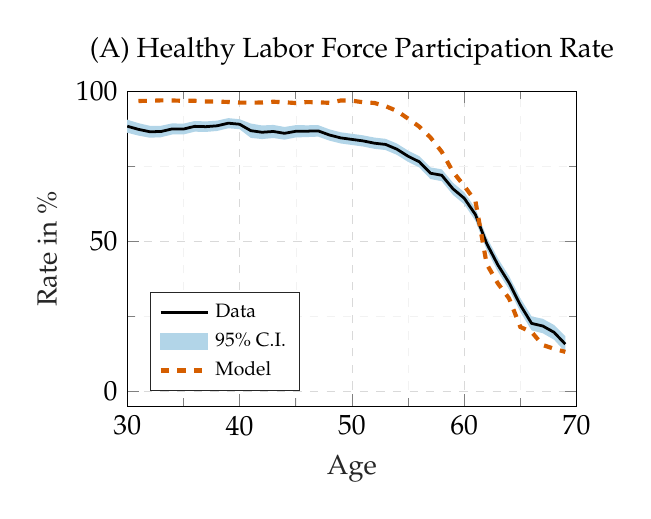
\begin{tikzpicture}
\begin{axis}[%
scale only axis,
width=5.706cm,
height=4cm,
at={(0cm,0cm)},
xmin=30,
xmax=70,
xlabel style={font=\color{white!15!black}},
xlabel={Age},
ymin=-5,
ymax=100,
ymajorgrids=true,
grid style=dashed,
ylabel style={font=\color{white!15!black}},
ylabel={Rate in \%},
axis background/.style={fill=white},
%title style={font=\bfseries},
title={(A) Healthy Labor Force Participation Rate},
legend style={at={(axis cs:32,0)}, anchor=south west, legend cell align=left, align=left, draw=white!15!black, font=\scriptsize},
grid=both,
grid style={line width=0.2pt, draw=gray!30},
minor grid style={line width=0.1pt, draw=gray!10},
minor tick num=1
]

% Main line (lfprlr0) - blue solid line
\addplot [color=black, line width=1pt]
  table[row sep=crcr, y expr=\thisrowno{1}*100]{%
30 0.8833822\\
31 0.8728638\\
32 0.8650124\\
33 0.8656822\\
34 0.8743696\\
35 0.873809\\
36 0.8829339\\
37 0.8818902\\
38 0.8847443\\
39 0.8934818\\
40 0.8900082\\
41 0.8684802\\
42 0.8632262\\
43 0.8659114\\
44 0.8597141\\
45 0.8664337\\
46 0.866869\\
47 0.8677746\\
48 0.8541223\\
49 0.8445035\\
50 0.8394285\\
51 0.8343548\\
52 0.8268231\\
53 0.8226036\\
54 0.8069361\\
55 0.7833442\\
56 0.7647346\\
57 0.7266455\\
58 0.7198906\\
59 0.6746376\\
60 0.6433743\\
61 0.5887213\\
62 0.4924323\\
63 0.4207888\\
64 0.3610537\\
65 0.2870897\\
66 0.2260264\\
67 0.21724\\
68 0.1962348\\
69 0.1569484\\
% 70 0.1681354\\
% 71 0.121358\\
% 72 0.1394618\\
% 73 0.1092736\\
% 74 0.1141775\\
% 75 0.0792269\\
% 76 0.0917666\\
% 77 0.0850947\\
% 78 0.0388536\\
% 79 0.0336195\\
% 80 0.058109\\
% 81 0.016314\\
% 82 0.0270162\\
% 83 -0.0089496\\
% 84 0.0236253\\
% 85 -0.0178846\\
};
\addlegendentry{Data}

% Upper bound (standard error high)
\addplot[name path=upper, draw=none, forget plot] 
  table[row sep=crcr,y expr=\thisrowno{1}*100]{%
30 0.9051051\\
31 0.8935855\\
32 0.8848711\\
33 0.88477\\
34 0.892873\\
35 0.8917789\\
36 0.9007229\\
37 0.8994025\\
38 0.9019169\\
39 0.9103903\\
40 0.9066504\\
41 0.8923349\\
42 0.8859496\\
43 0.8876875\\
44 0.8808528\\
45 0.8869151\\
46 0.88653\\
47 0.8869081\\
48 0.8729149\\
49 0.863117\\
50 0.858066\\
51 0.8529794\\
52 0.8455561\\
53 0.8413141\\
54 0.8257702\\
55 0.8021987\\
56 0.7835673\\
57 0.7460628\\
58 0.739598\\
59 0.6947576\\
60 0.663489\\
61 0.6094228\\
62 0.5136542\\
63 0.4426488\\
64 0.3833388\\
65 0.3098885\\
66 0.2493425\\
67 0.2413235\\
68 0.2207975\\
69 0.1832494\\
% 70 0.194256\\
% 71 0.1491448\\
% 72 0.1675596\\
% 73 0.1396055\\
% 74 0.1450964\\
% 75 0.1120739\\
% 76 0.1273876\\
% 77 0.1228318\\
% 78 0.0783176\\
% 79 0.0761687\\
% 80 0.1034711\\
% 81 0.0718914\\
% 82 0.080405\\
% 83 0.0504064\\
% 84 0.082339\\
% 85 0.0525297\\
};

% Lower bound (standard error low)
\addplot[name path=lower, draw=none, forget plot] 
  table[row sep=crcr,y expr=\thisrowno{1}*100]{%
30 0.8616592\\
31 0.852142\\
32 0.8451536\\
33 0.8465945\\
34 0.8558661\\
35 0.855839\\
36 0.8651446\\
37 0.8643779\\
38 0.8675715\\
39 0.8765733\\
40 0.8733659\\
41 0.8446254\\
42 0.8405027\\
43 0.8441353\\
44 0.8385755\\
45 0.8459523\\
46 0.8472079\\
47 0.848641\\
48 0.8353298\\
49 0.8258898\\
50 0.8207909\\
51 0.81573\\
52 0.80809\\
53 0.8038934\\
54 0.788102\\
55 0.7644898\\
56 0.7459021\\
57 0.7072282\\
58 0.7001832\\
59 0.6545175\\
60 0.6232595\\
61 0.5680198\\
62 0.4712104\\
63 0.3989288\\
64 0.3387687\\
65 0.2642909\\
66 0.2027102\\
67 0.1931565\\
68 0.1716722\\
69 0.1306474\\
% 70 0.1420148\\
% 71 0.0935712\\
% 72 0.111364\\
% 73 0.0789419\\
% 74 0.0832585\\
% 75 0.04638\\
% 76 0.0561455\\
% 77 0.0473576\\
% 78 -0.0006104\\
% 79 -0.0089297\\
% 80 0.012747\\
% 81 -0.0392634\\
% 82 -0.0263728\\
% 83 -0.0683057\\
% 84 -0.0350885\\
% 85 -0.0882989\\
};

% Fill between the paths
\addplot[blue!30] fill between[of=upper and lower];
\addlegendentry{95\% C.I.}

\addplot [color=red, line width=1.5pt, dashed]
  table[row sep=crcr,y expr=\thisrowno{1}*100]{%
age1	hlfprs	
30	0.968957203	\\
31	0.967528563	\\
32	0.968149038	\\
33	0.969477183	\\
34	0.969174977	\\
35	0.968055978	\\
36	0.96822487	\\
37	0.965898618	\\
38	0.965400062	\\
39	0.964252409	\\
40	0.962068966	\\
41	0.962097284	\\
42	0.962270133	\\
43	0.964990452	\\
44	0.963176433	\\
45	0.960663199	\\
46	0.963867188	\\
47	0.963036304	\\
48	0.961359094	\\
49	0.969137873	\\
50	0.968557758	\\
51	0.963202726	\\
52	0.960872576	\\
53	0.95022783	\\
54	0.934327299	\\
55	0.908797127	\\
56	0.881924198	\\
57	0.845669874	\\
58	0.798134328	\\
59	0.731264194	\\
60	0.684393064	\\
61	0.633671083	\\
62	0.423769508	\\
63	0.359203576	\\
64	0.308793456	\\
65	0.213959285	\\
66	0.197284684	\\
67	0.153846154	\\
68	0.141542507	\\
69	0.131132917	\\
  };
\addlegendentry{Model}

\end{axis}
\end{tikzpicture} & 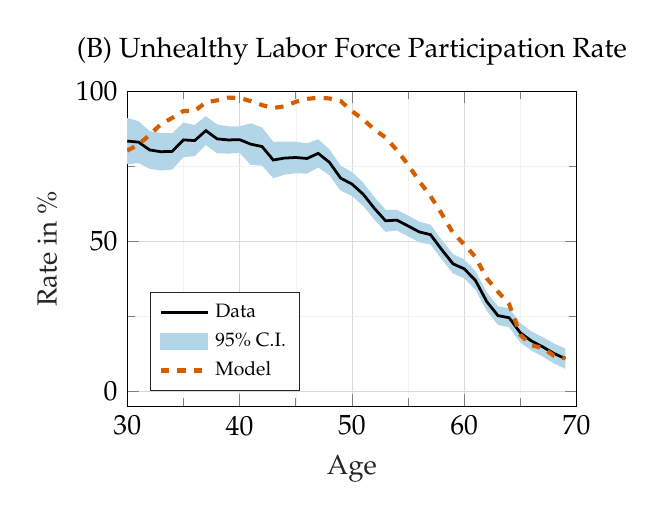
\begin{tikzpicture}
\begin{axis}[%
width=5.706cm,
height=4cm,
at={(0cm,0cm)},
scale only axis,
xmin=30,
xmax=70,
xlabel style={font=\color{white!15!black}},
xlabel={Age},
ymin=-5,
ymax=100,
ylabel style={font=\color{white!15!black}},
ylabel={Rate in \%},
axis background/.style={fill=white},
%title style={font=\bfseries},
title={(B) Unhealthy Labor Force Participation Rate},
legend style={at={(axis cs:32,0)}, anchor=south west, legend cell align=left, align=left, draw=white!15!black, font=\scriptsize},
grid=both,
grid style={line width=0.2pt, draw=gray!30},
minor grid style={line width=0.1pt, draw=gray!10},
minor tick num=1
]

% Main line (lfprlr0) - blue solid line
\addplot [color=black, line width=1pt]
  table[row sep=crcr,y expr=\thisrowno{1}*100]{%
30 0.8339695\\
31 0.830355\\
32 0.8042343\\
33 0.7983715\\
34 0.7995418\\
35 0.8378634\\
36 0.8354884\\
37 0.8686402\\
38 0.8411449\\
39 0.8375973\\
40 0.8386171\\
41 0.8234905\\
42 0.8157026\\
43 0.7707186\\
44 0.7771355\\
45 0.7791017\\
46 0.7758368\\
47 0.7928331\\
48 0.762918\\
49 0.710295\\
50 0.6906397\\
51 0.6569952\\
52 0.6095482\\
53 0.5680759\\
54 0.5703449\\
55 0.5509109\\
56 0.5310219\\
57 0.5219091\\
58 0.4718995\\
59 0.4247883\\
60 0.4079395\\
61 0.3693248\\
62 0.2990521\\
63 0.2519826\\
64 0.2448949\\
65 0.1944834\\
66 0.1670593\\
67 0.1475739\\
68 0.1256826\\
69 0.1083655\\
% 70 0.1681354\\
% 71 0.121358\\
% 72 0.1394618\\
% 73 0.1092736\\
% 74 0.1141775\\
% 75 0.0792269\\
% 76 0.0917666\\
% 77 0.0850947\\
% 78 0.0388536\\
% 79 0.0336195\\
% 80 0.058109\\
% 81 0.016314\\
% 82 0.0270162\\
% 83 -0.0089496\\
% 84 0.0236253\\
% 85 -0.0178846\\
};
\addlegendentry{Data}

% Upper bound (standard error high)
\addplot[name path=upper, draw=none, forget plot] 
  table[row sep=crcr,y expr=\thisrowno{1}*100]{%
30 0.9111052\\
31 0.9001306\\
32 0.8669667\\
33 0.8606798\\
34 0.860257\\
35 0.8955216\\
36 0.8874309\\
37 0.9166927\\
38 0.8892378\\
39 0.8830312\\
40 0.8826435\\
41 0.8928777\\
42 0.8792804\\
43 0.8314206\\
44 0.83197\\
45 0.8315616\\
46 0.8263692\\
47 0.8398106\\
48 0.8062539\\
49 0.7522238\\
50 0.7306355\\
51 0.6956045\\
52 0.6471571\\
53 0.6047442\\
54 0.6048974\\
55 0.5855613\\
56 0.5653728\\
57 0.5550599\\
58 0.5043322\\
59 0.4570315\\
60 0.4391904\\
61 0.4005467\\
62 0.3297285\\
63 0.2832072\\
64 0.2764793\\
65 0.2267636\\
66 0.1990062\\
67 0.1796762\\
68 0.1588332\\
69 0.142154\\
% 70 0.194256\\
% 71 0.1491448\\
% 72 0.1675596\\
% 73 0.1396055\\
% 74 0.1450964\\
% 75 0.1120739\\
% 76 0.1273876\\
% 77 0.1228318\\
% 78 0.0783176\\
% 79 0.0761687\\
% 80 0.1034711\\
% 81 0.0718914\\
% 82 0.080405\\
% 83 0.0504064\\
% 84 0.082339\\
% 85 0.0525297\\
};

% Lower bound (standard error low)
\addplot[name path=lower, draw=none, forget plot] 
  table[row sep=crcr,y expr=\thisrowno{1}*100]{%
30 0.7568338\\
31 0.7605796\\
32 0.7415019\\
33 0.7360631\\
34 0.7388266\\
35 0.7802051\\
36 0.7835459\\
37 0.8205878\\
38 0.7930518\\
39 0.7921634\\
40 0.7945906\\
41 0.7541034\\
42 0.7521245\\
43 0.7100167\\
44 0.7223011\\
45 0.7266418\\
46 0.7253045\\
47 0.7458558\\
48 0.719582\\
49 0.6683661\\
50 0.6506439\\
51 0.618386\\
52 0.5719393\\
53 0.5314076\\
54 0.5357924\\
55 0.5162606\\
56 0.496671\\
57 0.4887584\\
58 0.4394668\\
59 0.3925449\\
60 0.3766887\\
61 0.3381029\\
62 0.2683756\\
63 0.2207581\\
64 0.2133105\\
65 0.1622031\\
66 0.1351124\\
67 0.1154717\\
68 0.092532\\
69 0.0745769\\
% 70 0.1420148\\
% 71 0.0935712\\
% 72 0.111364\\
% 73 0.0789419\\
% 74 0.0832585\\
% 75 0.04638\\
% 76 0.0561455\\
% 77 0.0473576\\
% 78 -0.0006104\\
% 79 -0.0089297\\
% 80 0.012747\\
% 81 -0.0392634\\
% 82 -0.0263728\\
% 83 -0.0683057\\
% 84 -0.0350885\\
% 85 -0.0882989\\
};

% Fill between the paths
\addplot[blue!30] fill between[of=upper and lower];
\addlegendentry{95\% C.I.}

\addplot [color=red, line width=1.5pt, dashed]
  table[row sep=crcr,y expr=\thisrowno{1}*100]{%
30	0.802197802	\\
31	0.82183908	\\
32	0.854651163	\\
33	0.890052356	\\
34	0.910994764	\\
35	0.9342723	\\
36	0.933920705	\\
37	0.963265306	\\
38	0.969581749	\\
39	0.978798587	\\
40	0.977419355	\\
41	0.967065868	\\
42	0.953757225	\\
43	0.944134078	\\
44	0.949602122	\\
45	0.964622642	\\
46	0.974299065	\\
47	0.978723404	\\
48	0.975903614	\\
49	0.967244701	\\
50	0.933797909	\\
51	0.90619469	\\
52	0.87254902	\\
53	0.845440495	\\
54	0.803806735	\\
55	0.755244755	\\
56	0.69973545	\\
57	0.65037594	\\
58	0.591463415	\\
59	0.527972028	\\
60	0.489502762	\\
61	0.447537473	\\
62	0.376623377	\\
63	0.332050048	\\
64	0.290047393	\\
65	0.187557182	\\
66	0.153105862	\\
67	0.143564356	\\
68	0.118226601	\\
69	0.109697933	\\
  };
\addlegendentry{Model};

\end{axis}
\end{tikzpicture} \\[1ex]
% EDITED (MVPF paper, revision pass): axis range and legend placement only: ymin/ymax -5/10 -> -1/5; legend moved to the upper left (axis cs:31,4.8, anchor north west). Data unchanged.
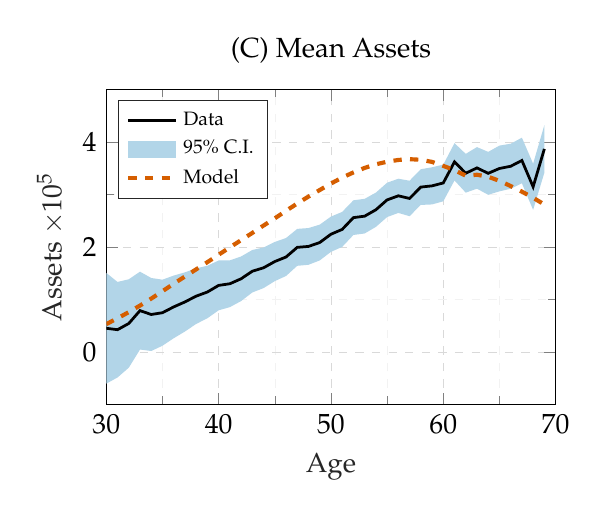
\begin{tikzpicture}
\begin{axis}[%
scale only axis,
width=5.706cm,
height=4cm,
at={(0cm,0cm)},
ylabel={Short label\phantom{(extra)}},
xmin=30,
xmax=70,
xlabel style={font=\color{white!15!black}},
xlabel={Age},
ymin=-1,
ymax=5,
ymajorgrids=true,
grid style=dashed,
ylabel style={font=\color{white!15!black}},
ylabel={Assets $\times10^5$},
axis background/.style={fill=white},
%title style={font=\bfseries},
title={(C) Mean Assets},
legend style={at={(axis cs:31,4.8)}, anchor=north west, legend cell align=left, align=left, draw=white!15!black, font=\scriptsize},
grid=both,
grid style={line width=0.2pt, draw=gray!30},
minor grid style={line width=0.1pt, draw=gray!10},
minor tick num=1
]

% Main line (lfprlr0) - blue solid line
\addplot [color=black, line width=1pt]
  table[row sep=crcr]{%, y expr=\thisrowno{1}*100]{%
30	0.44883396	\\
31	0.42199558	\\
32	0.54018803	\\
33	0.78561033	\\
34	0.71175356	\\
35	0.74541797	\\
36	0.85600565	\\
37	0.95088265	\\
38	1.0613716	\\
39	1.1398318	\\
40	1.2659439	\\
41	1.2972758	\\
42	1.3919758	\\
43	1.535846	\\
44	1.6013677	\\
45	1.7205047	\\
46	1.8064766	\\
47	1.9908018	\\
48	2.0085264	\\
49	2.0823645	\\
50	2.2407959	\\
51	2.3326437	\\
52	2.556798	\\
53	2.5850001	\\
54	2.7065999	\\
55	2.8947089	\\
56	2.9723681	\\
57	2.9223428	\\
58	3.1388551	\\
59	3.1621034	\\
60	3.2175482	\\
61	3.620027	\\
62	3.4022311	\\
63	3.50429	\\
64	3.4009493	\\
65	3.4932815	\\
66	3.5353909	\\
67	3.6457606	\\
68	3.1442149	\\
69	3.8660995	\\
};
\addlegendentry{Data}

% Upper bound (standard error high)
\addplot[name path=upper, draw=none, forget plot] 
  table[row sep=crcr]{%,y expr=\thisrowno{1}*100]{%
%age1	plus2se	
30	1.5034447	\\
31	1.3318214	\\
32	1.3825211	\\
33	1.5269781	\\
34	1.4072133	\\
35	1.3745624	\\
36	1.4530003	\\
37	1.5145966	\\
38	1.5909592	\\
39	1.6398946	\\
40	1.7404519	\\
41	1.742667	\\
42	1.8167697	\\
43	1.9404281	\\
44	1.9883948	\\
45	2.0936916	\\
46	2.1680532	\\
47	2.3425176	\\
48	2.3583419	\\
49	2.4231668	\\
50	2.5766613	\\
51	2.6659567	\\
52	2.8871246	\\
53	2.9148088	\\
54	3.0332248	\\
55	3.2218368	\\
56	3.2981602	\\
57	3.260209	\\
58	3.4790351	\\
59	3.5159971	\\
60	3.5670526	\\
61	3.9753495	\\
62	3.7715802	\\
63	3.9004755	\\
64	3.8095388	\\
65	3.92889	\\
66	3.964179	\\
67	4.080106	\\
68	3.5837879	\\
69	4.3190544	\\
};

% Lower bound (standard error low)
\addplot[name path=lower, draw=none, forget plot] 
  table[row sep=crcr]{%,y expr=\thisrowno{1}*100]{%
%age1	minus2se	
30	-0.60577681	\\
31	-0.48783214	\\
32	-0.3021432	\\
33	0.04424252	\\
34	0.01629566	\\
35	0.11627356	\\
36	0.25901103	\\
37	0.38716866	\\
38	0.53178403	\\
39	0.63977097	\\
40	0.79143593	\\
41	0.85188656	\\
42	0.96718204	\\
43	1.1312658	\\
44	1.2143407	\\
45	1.347316	\\
46	1.4449018	\\
47	1.639086	\\
48	1.6587109	\\
49	1.7415622	\\
50	1.9049305	\\
51	1.9993306	\\
52	2.2264713	\\
53	2.2551913	\\
54	2.379975	\\
55	2.567581	\\
56	2.6465741	\\
57	2.5844784	\\
58	2.798675	\\
59	2.8082117	\\
60	2.8680457	\\
61	3.2647044	\\
62	3.032882	\\
63	3.1081044	\\
64	2.9923581	\\
65	3.057673	\\
66	3.1066009	\\
67	3.2114152	\\
68	2.7046419	\\
69	3.4131445	\\
};

% Fill between the paths
\addplot[blue!30] fill between[of=upper and lower];
\addlegendentry{95\% C.I.}

\addplot [color=red, line width=1.5pt, dashed]
  table[row sep=crcr]{%,y expr=\thisrowno{1}*100]{%
%age1	means	
30		0.52848903	\\
31		0.63949028	\\
32		0.75641608	\\
33		0.88135533	\\
34		1.0146479	\\
35		1.15531	\\
36		1.2980178	\\
37		1.4347526	\\
38		1.5716783	\\
39		1.7089924	\\
40		1.8504481	\\
41		1.990505	\\
42		2.1279477	\\
43		2.2655075	\\
44		2.4060401	\\
45		2.543429	\\
46		2.6864321	\\
47		2.8260226	\\
48		2.9579886	\\
49		3.0826261	\\
50		3.2063248	\\
51		3.3196893	\\
52		3.418323	\\
53		3.503818	\\
54		3.572795	\\
55		3.6217814	\\
56		3.6555198	\\
57		3.6704038	\\
58		3.6589162	\\
59		3.6182893	\\
60		3.5423121	\\
61		3.4621445	\\
62		3.3563867	\\
63		3.3740218	\\
64		3.3360893	\\
65		3.2575333	\\
66		3.15897	\\
67		3.0522143	\\
68		2.9347336	\\
69		2.8075372	\\
  };
\addlegendentry{Model};

\end{axis}
\end{tikzpicture} & % EDITED (MVPF paper, revision pass): axis range and legend placement only: ymin/ymax -5/10 -> -1/5; legend moved to the upper left (axis cs:31,4.8, anchor north west). Data unchanged.
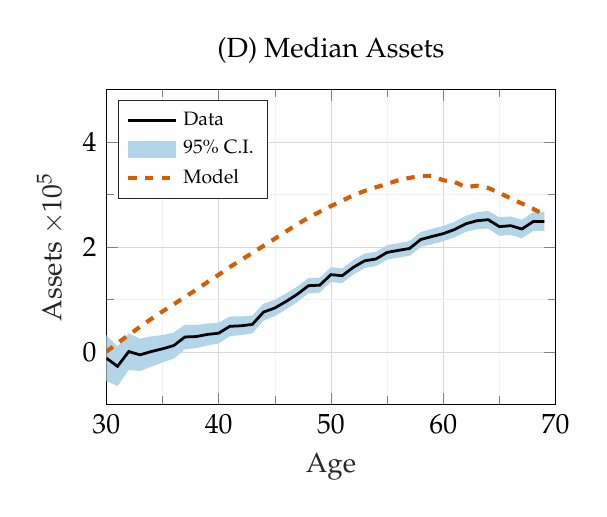
\begin{tikzpicture}
\begin{axis}[%
width=5.706cm,
height=4cm,
at={(0cm,0cm)},
scale only axis,
xmin=30,
xmax=70,
xlabel style={font=\color{white!15!black}},
xlabel={Age},
ymin=-1,
ymax=5,
ylabel style={font=\color{white!15!black}},
ylabel={Assets $\times10^5$},
axis background/.style={fill=white},
%title style={font=\bfseries},
title={(D) Median Assets},
legend style={at={(axis cs:31,4.8)}, anchor=north west, legend cell align=left, align=left, draw=white!15!black, font=\scriptsize},
grid=both,
grid style={line width=0.2pt, draw=gray!30},
minor grid style={line width=0.1pt, draw=gray!10},
minor tick num=1
]

% Main line (lfprlr0) - blue solid line
\addplot [color=black, line width=1pt]
  table[row sep=crcr]{%, y expr=\thisrowno{1}*100]{%
30	-0.11895441	\\
31	-0.27639282	\\
32	0.0054679	\\
33	-0.05680846	\\
34	0.00530582	\\
35	0.05775673	\\
36	0.11935496	\\
37	0.283448	\\
38	0.29103227	\\
39	0.3317854	\\
40	0.3554958	\\
41	0.48654667	\\
42	0.49660314	\\
43	0.5230298	\\
44	0.75761317	\\
45	0.83516986	\\
46	0.95970209	\\
47	1.09713	\\
48	1.2602245	\\
49	1.2697649	\\
50	1.4709074	\\
51	1.4499263	\\
52	1.6115453	\\
53	1.7346132	\\
54	1.768639	\\
55	1.894712	\\
56	1.932978	\\
57	1.9691985	\\
58	2.1408199	\\
59	2.198014	\\
60	2.2522161	\\
61	2.329607	\\
62	2.4388831	\\
63	2.4980613	\\
64	2.5174607	\\
65	2.3850927	\\
66	2.403937	\\
67	2.3398796	\\
68	2.4810502	\\
69	2.4844838	\\
};
\addlegendentry{Data}

% Upper bound (standard error high)
\addplot[name path=upper, draw=none, forget plot] 
  table[row sep=crcr]{%,y expr=\thisrowno{1}*100]{%
30	0.31699318	\\
31	0.10011389	\\
32	0.35445438	\\
33	0.2506089	\\
34	0.29365724	\\
35	0.31921015	\\
36	0.36788288	\\
37	0.51851016	\\
38	0.51206232	\\
39	0.54050287	\\
40	0.55375253	\\
41	0.6729007	\\
42	0.67474134	\\
43	0.69266526	\\
44	0.9196122	\\
45	0.99146252	\\
46	1.1109516	\\
47	1.2443443	\\
48	1.4066153	\\
49	1.4124912	\\
50	1.6117372	\\
51	1.5897184	\\
52	1.74986	\\
53	1.8723206	\\
54	1.9050796	\\
55	2.0317431	\\
56	2.069126	\\
57	2.1103524	\\
58	2.2830432	\\
59	2.3452282	\\
60	2.3976214	\\
61	2.4770057	\\
62	2.5911442	\\
63	2.660554	\\
64	2.6842085	\\
65	2.563393	\\
66	2.5792043	\\
67	2.5160896	\\
68	2.66001	\\
69	2.6677378	\\
};

% Lower bound (standard error low)
\addplot[name path=lower, draw=none, forget plot] 
  table[row sep=crcr]{%,y expr=\thisrowno{1}*100]{%
30	-0.55490014	\\
31	-0.65290139	\\
32	-0.34352043	\\
33	-0.36422581	\\
34	-0.28304559	\\
35	-0.20369669	\\
36	-0.12917297	\\
37	0.04838584	\\
38	0.07000223	\\
39	0.12306792	\\
40	0.15724093	\\
41	0.30019264	\\
42	0.31846681	\\
43	0.35339433	\\
44	0.595616	\\
45	0.6788772	\\
46	0.80845444	\\
47	0.94991389	\\
48	1.1138318	\\
49	1.1270405	\\
50	1.3300777	\\
51	1.3101343	\\
52	1.4732306	\\
53	1.5969077	\\
54	1.6321967	\\
55	1.757679	\\
56	1.79683	\\
57	1.8280445	\\
58	1.9985966	\\
59	2.0507979	\\
60	2.1068127	\\
61	2.1822064	\\
62	2.2866238	\\
63	2.3355686	\\
64	2.3507148	\\
65	2.2067924	\\
66	2.2286696	\\
67	2.1636714	\\
68	2.3020905	\\
69	2.3012316	\\
};

% Fill between the paths
\addplot[blue!30] fill between[of=upper and lower];
\addlegendentry{95\% C.I.}

\addplot [color=red, line width=1.5pt, dashed]
  table[row sep=crcr]{%,y expr=\thisrowno{1}*100]{%
30	0	\\
31	0.16779459	\\
32	0.32122598	\\
33	0.4767707	\\
34	0.62655105	\\
35	0.76897051	\\
36	0.90586907	\\
37	1.0457174	\\
38	1.1805579	\\
39	1.3286312	\\
40	1.4692509	\\
41	1.6162862	\\
42	1.7495322	\\
43	1.8845477	\\
44	2.0202169	\\
45	2.155189	\\
46	2.2940789	\\
47	2.4300734	\\
48	2.5560681	\\
49	2.6679432	\\
50	2.777585	\\
51	2.8791545	\\
52	2.9829276	\\
53	3.0654487	\\
54	3.1348877	\\
55	3.1996158	\\
56	3.2695508	\\
57	3.3144833	\\
58	3.3506717	\\
59	3.3531731	\\
60	3.2686488	\\
61	3.2387078	\\
62	3.1352764	\\
63	3.1648646	\\
64	3.1213115	\\
65	3.0298607	\\
66	2.923937	\\
67	2.8263209	\\
68	2.7256512	\\
69	2.6072655	\\
  };
\addlegendentry{Model};

\end{axis}
\end{tikzpicture}
\end{tabular}
\tabnotes{\textit{Notes:} Panels A and B show labor force participation rates (percent) of healthy individuals ($h=0$) and unhealthy individuals (poor health or disability, $h\in\{1,2\}$); panels C and D show mean and median nonpension assets (hundreds of thousands of 2016 dollars). Solid lines are data profiles estimated from the Panel Study of Income Dynamics, shaded areas are 95\% confidence intervals, and dashed lines are profiles simulated from the model with logarithmic utility at the estimates of \autoref{tab:lnc}. Compared with the baseline (\autoref{fig:fit_labor} and \autoref{fig:fit_assets}), the logarithmic specification fits assets at older ages better and participation worse.}
\end{figure}

% ============================================================================
%  Appendix D: Construction of Reforms and Outcomes
%  Sources: FROT 2025_sub/12_app_quant.tex ("Reforms": Construction of Reforms,
%  Construction of Outcomes); 2025_sub/7_policy_reforms.tex (notes to the table of
%  elimination experiments); tables/DRC_visualization_4.tex (claiming schedules).
% ============================================================================
\section{Construction of Reforms and Outcomes}\label{app:reforms}

This appendix describes how each instrument-elimination experiment and each reform is implemented and how its welfare, fiscal, MVPF, and participation outcomes are computed. Every reform is a permanent change in the rules of Section~\ref{sec:model} that the cohort knows from age 30. For each reform, we solve the model again by backward induction under the new rules (Appendix~\ref{app:solution}) and simulate the cohort forward from the same initial distribution as in the status quo. All other rules and parameters keep their status-quo values, and the wage profiles and the pretax return $r_f$ are held fixed. Outcomes are computed from the simulated histories.

\subsection{Instrument-Elimination Experiments}

The five experiments of \autoref{tab:elim} each remove one instrument from the estimated economy.
\begin{itemize}
\item \textit{D1, no Social Security benefits:} Social Security benefits are set to zero. In a variant reported in Section~\ref{sec:results_elim}, only retirement benefits are set to zero and disability benefits are kept.
\item \textit{D2, loss from incomplete coverage in Medicare:} out-of-pocket medical expenses after age 65 are set to zero for participants and nonparticipants, so that all medical expenditures after 65 are covered. The table reports the welfare change of the status quo relative to this economy, which, by the antisymmetry of the CE, is minus the welfare gain from full coverage.
\item \textit{D3, full savings subsidy:} the net return on assets $r$ is set equal to the pretax return $r_f$. This experiment coincides with reform K3.
\item \textit{D4, no income tax:} the income tax $T_t(\cdot)$ of \eqref{eq:tax} is set to zero at every age.
\item \textit{D5, no disability benefits:} DI benefits $db_t$ of \eqref{eq:di} are set to zero.
\end{itemize}
These experiments change the government budget without financing the change. We report their CE and LE welfare changes only.

\subsection{Claiming-Age Dependence}

Let $\alpha(a)=b(a)/PIA$ be the benefit, as a fraction of the PIA, of an individual who claims at age $a\in\{62,\ldots,70\}$. Under the rules of the status quo and of the AN and AD reforms,
\begin{equation*}
\alpha(a)=
\begin{cases}
1-\dfrac{1}{15}\min\{\mathit{NRA}-a,\,3\}-\dfrac{1}{20}\max\{\mathit{NRA}-a-3,\,0\} & \text{if } a<\mathit{NRA},\\[2ex]
1+\delta\,(a-\mathit{NRA}) & \text{if } a\geq \mathit{NRA}:
\end{cases}
\end{equation*}
benefits fall by $6\tfrac{2}{3}$ percent of the PIA for each of the first three years by which the claim precedes the NRA and by 5 percent for each additional year, and they rise by the DRC $\delta$ for each year of delay past the NRA. The status quo (AN0) has $\mathit{NRA}=65$ and $\delta=4.5$ percent. % Reductions of 6.67% (first three years) and 5% (earlier years): FROT 2025_sub/12_app_quant.tex (commented rule text in 'Reforms of Social Security Claiming-Age Dependence') and tables/DRC_visualization_4.tex.
\begin{itemize}
\item \textit{AN1--AN3:} $\mathit{NRA}=66$, 67, and 68, with $\delta=4.5$ percent. The schedule shifts to the right by one, two, and three years, so that the benefit at 62 falls from 80 to 75, 70, and 65 percent of the PIA. Because DI benefits are paid until the NRA \eqref{eq:di}, they are paid until the new NRA.
\item \textit{AD1--AD5:} $\mathit{NRA}=65$ and $\delta=8$, 8.5, 9, 9.5, and 10 percent. Benefits for claims before the NRA are unchanged.
\item \textit{AL1--AL9:} $\alpha(a)=1+x\,(a-65)$ at every claiming age, with $x=7,8,\ldots,15$ percent. The reduction for early claiming and the credit for delay are equal in absolute value.
\end{itemize}
\autoref{tab:schedules} reports $\alpha(a)$, in percent, for every claiming age and every reform; \autoref{fig:schedules} plots selected schedules. The adjustments of the AN reforms follow the rules of the Social Security Administration for the corresponding NRA.

\begin{table}[!htbp]
\centering
\caption{Benefits by Claiming Age under the Claiming-Age Reforms}\label{tab:schedules}
\small
% Source: FROT tables/DRC_visualization_4.tex (program rules; benefit as % of PIA by claiming age).
% Values copied exactly as printed in the source; only the formatting (booktabs, no color gradient) differs.
\begin{tabular}{@{}l l c c c c c c c c c@{}}
\toprule
 & & \multicolumn{9}{c}{Claiming age} \\
\cmidrule(l){3-11}
 & Schedule & 62 & 63 & 64 & 65 & 66 & 67 & 68 & 69 & 70 \\
\midrule
(AN0) & Status quo (NRA 65) & 80 & 86.67 & 93.33 & \textbf{100} & 104.5 & 109 & 113.5 & 118 & 122.5 \\
\addlinespace
\multicolumn{11}{@{}l}{\textit{A. Raising the normal retirement age (NRA)}} \\
(AN1) & NRA at 66 & 75 & 80 & 86.67 & 93.33 & \textbf{100} & 104.5 & 109 & 113.5 & 118 \\
(AN2) & NRA at 67 & 70 & 75 & 80 & 86.67 & 93.33 & \textbf{100} & 104.5 & 109 & 113.5 \\
(AN3) & NRA at 68 & 65 & 70 & 75 & 80 & 86.67 & 93.33 & \textbf{100} & 104.5 & 109 \\
\addlinespace
\multicolumn{11}{@{}l}{\textit{B. Raising the delayed retirement credit (DRC)}} \\
(AD1) & DRC at 8\% & 80 & 86.67 & 93.33 & \textbf{100} & 108 & 116 & 124 & 132 & 140 \\
(AD2) & DRC at 8.5\% & 80 & 86.67 & 93.33 & \textbf{100} & 108.5 & 117 & 125.5 & 134 & 142.5 \\
(AD3) & DRC at 9\% & 80 & 86.67 & 93.33 & \textbf{100} & 109 & 118 & 127 & 136 & 145 \\
(AD4) & DRC at 9.5\% & 80 & 86.67 & 93.33 & \textbf{100} & 109.5 & 119 & 128.5 & 138 & 147.5 \\
(AD5) & DRC at 10\% & 80 & 86.67 & 93.33 & \textbf{100} & 110 & 120 & 130 & 140 & 150 \\
\addlinespace
\multicolumn{11}{@{}l}{\textit{C. Symmetric adjustment around the NRA of 65}} \\
(AL1) & Linear $\pm$7\% & 79 & 86 & 93 & \textbf{100} & 107 & 114 & 121 & 128 & 135 \\
(AL2) & Linear $\pm$8\% & 76 & 84 & 92 & \textbf{100} & 108 & 116 & 124 & 132 & 140 \\
(AL3) & Linear $\pm$9\% & 73 & 82 & 91 & \textbf{100} & 109 & 118 & 127 & 136 & 145 \\
(AL4) & Linear $\pm$10\% & 70 & 80 & 90 & \textbf{100} & 110 & 120 & 130 & 140 & 150 \\
(AL5) & Linear $\pm$11\% & 67 & 78 & 89 & \textbf{100} & 111 & 122 & 133 & 144 & 155 \\
(AL6) & Linear $\pm$12\% & 64 & 76 & 88 & \textbf{100} & 112 & 124 & 136 & 148 & 160 \\
(AL7) & Linear $\pm$13\% & 61 & 74 & 87 & \textbf{100} & 113 & 126 & 139 & 152 & 165 \\
(AL8) & Linear $\pm$14\% & 58 & 72 & 86 & \textbf{100} & 114 & 128 & 142 & 156 & 170 \\
(AL9) & Linear $\pm$15\% & 55 & 70 & 85 & \textbf{100} & 115 & 130 & 145 & 160 & 175 \\
\bottomrule
\end{tabular}

\tabnotes{\textit{Notes:} Retirement benefit received by an individual who claims at each age from 62 to 70, in percent of the primary insurance amount (PIA). Bold entries mark the normal retirement age (NRA), at which the benefit equals the PIA. AN0: status quo of the 1920--1940 birth cohorts, with an NRA of 65, a reduction of $6\tfrac{2}{3}$ percent of the PIA per year of claiming before the NRA, and a delayed retirement credit (DRC) of 4.5 percent of the PIA per year of claiming after the NRA. AN1--AN3 raise the NRA to 66, 67, and 68; the reduction is $6\tfrac{2}{3}$ percent per year for the three years before the NRA and 5 percent per year before that. AD1--AD5 raise the DRC to 8, 8.5, 9, 9.5, and 10 percent. AL1--AL9 set the reduction for early claiming and the DRC to a common rate of 7 to 15 percent per year. \textit{Source:} rules of the Social Security Administration for the status quo and the AN reforms; authors' construction for the AD and AL reforms.}
\end{table}

\subsection{Benefit Progressivity and Level}

Write the PIA formula \eqref{eq:pia} with replacement rates $\omega=(\omega_1,\omega_2,\omega_3)$:
\begin{equation*}
\begin{split}
PIA_t={}&\omega_1\min\{aime_t,aime_0\}+\omega_2\min\big\{\max\{aime_t-aime_0,0\},\,aime_1-aime_0\big\}\\
&+\omega_3\max\{aime_t-aime_1,0\},
\end{split}
\end{equation*}
with $\omega=(0.90,\,0.32,\,0.15)$ in the status quo. The bend points $aime_0$ and $aime_1$ and the claiming-age adjustments are unchanged. The reforms set:
\begin{itemize}
\item \textit{P1.1--P1.9:} $\omega=(0.90+0.01k,\;0.32,\;0.15)$ for $k=1,\ldots,9$, which raises the first rate by one percentage point per step, from 0.91 to 0.99.
\item \textit{P2.0--P2.9:} $\omega=\big(0.99,\;0.32\,(1.01+0.01k),\;0.15\big)$ for $k=0,\ldots,9$, which raises the second rate by 0.32 percentage points (1 percent of its initial value) per step, from 0.3232 to 0.352, on top of the first rate of P1.9.
\item \textit{P3.0--P3.9:} $\omega=\big(0.99,\;0.352,\;0.15\,(1.01+0.01k)\big)$ for $k=0,\ldots,9$, which raises the third rate by 0.15 percentage points (1 percent of its initial value) per step, from 0.1515 to 0.165, on top of the first two rates of P2.9.
\item \textit{L0--L9:} $\omega=(1.01+0.01k)\times(0.90,\;0.32,\;0.15)$ for $k=0,\ldots,9$, which raises all three rates proportionally by 1 to 10 percent; L0 sets $\omega=(0.909,\,0.3232,\,0.1515)$ and L9 sets $\omega=(0.99,\,0.352,\,0.165)$.
\end{itemize}
The P reforms trace a path from the status quo to a 10 percent increase in all three rates that raises the brackets one at a time, from the bottom up. The path ends at the formula of L9: P3.9 and L9 set the same rates, and their simulated outcomes in \autoref{tab:generosity} and \autoref{tab:generosity_app} coincide.

\subsection{Medicare}

To implement the Medicare reforms, we first measure from the MEPS the average share of medical expenditures that Medicare covers for individuals aged 65 and older, by health status and working status. Denote this coverage rate by $q(h,P)$. At ages $t\geq65$, out-of-pocket medical expenses are $m_t=\big(1-q(h_t,P_t)\big)\,m^{tot}_t$, where $m^{tot}_t$ is total medical expenditure, and Medicare pays $m^{G}_t=q(h_t,P_t)\,m^{tot}_t$ (Section~\ref{sec:model_medical}). We simulate the estimated model with these coverage rates and use the simulated economy as the baseline for the two Medicare reforms.
\begin{itemize}
\item \textit{Part A:} the coverage rate of every individual aged 65 and older rises by 20 percentage points, $q(h,P)\to q(h,P)+0.20$, which represents expanded coverage of inpatient services. The targeted beneficiaries are all individuals aged 65 and older.
\item \textit{Part B:} the coverage rate of nonparticipants aged 65 and older rises by 20 percentage points, $q(h,0)\to q(h,0)+0.20$, which represents expanded coverage of physician and outpatient services. Because most employer-provided health insurance plans already cover these services, the reform targets nonparticipants. % Source: FROT 2025_sub/7_policy_reforms.tex, paragraph 'Medicare Reforms'.
The targeted beneficiaries are the nonparticipants aged 65 and older.
\end{itemize}
At unchanged behavior, each reform shifts 20 percent of the total medical expenditure of the targeted beneficiaries from out-of-pocket expenses to Medicare. Under Part B, the shift is conditional on not working, so the reform also changes the return to work after 65.

\subsection{Old-Age Income Taxes}

Reforms I1--I5 lower income taxes from age 62 by raising the level parameter of the after-tax income schedule $y-T_t(y)=\lambda_t\,y^{1-\tau_t}$:
\begin{equation*}
\tilde\lambda_t=
\begin{cases}
\lambda_t & \text{if } t\leq 61,\\
\lambda_t+x\,(t-61) & \text{if } t\geq 62,
\end{cases}
\qquad x=0.01,\,0.02,\,0.03,\,0.04,\,0.05,
\end{equation*}
with the progressivity parameter $\tau_t$ unchanged. At age $t\geq62$, after-tax income rises at every income level by the proportion $x(t-61)/\lambda_t$, and the tax cut $x(t-61)\,y^{1-\tau_t}$ rises with income and with age. Individuals anticipate the reform from age 30.

\subsection{Savings Subsidies}

Reforms K1--K3 raise the net return on assets at every age from $r$ to $\tilde r=r+\Delta_K$, with $\Delta_K=0.2$, 0.4, and 0.8 percentage points. The government pays the additional return $\Delta_K a_t$ on assets held at every age, and the present value of the subsidy is
\begin{equation*}
K=\sum_{t=30}^{T}(1+r)^{-(t-62)}\,\overline{\Delta_K a_t},
\end{equation*}
where the bar denotes the per capita value in the simulated cohort under the reform. Since $r=(1-\tau_k)\,r_f$ with $r_f=4$ percent and $\tau_k=20$ percent, the three subsidies are equivalent to lowering the capital-tax wedge $\tau_k$ to 15, 10, and 0 percent (exact arithmetic: $(1-\tilde\tau_k)\times 4=3.4$, 3.6, and 4.0 percent). K3 sets the net return equal to the pretax return and coincides with experiment D3.

\subsection{Construction of Outcomes}\label{app:outcomes}

\paragraph{Welfare.} Let $\bar V^{j}=\frac{1}{N}\sum_{i=1}^{N}V_{30}(X^{i}_{30};j)$ be the average value at age 30 over the $N$ simulated individuals under the rules $j$, where $j=0$ denotes the baseline and $j=1$ the reform; the initial states $X^{i}_{30}$ are the same under both. Because flow utility satisfies $u(e^{x}c,l)=e^{\gamma(1-\nu)x}u(c,l)$, scaling consumption in the baseline allocation by $e^{x}$ at every age and in every state multiplies $\bar V^{0}$ by $e^{\gamma(1-\nu)x}$. The consumption-equivalent welfare change is the $x$ that solves $\bar V^{1}=e^{\gamma(1-\nu)x}\bar V^{0}$, and the leisure-equivalent change the $y$ that solves $\bar V^{1}=e^{(1-\gamma)(1-\nu)y}\bar V^{0}$:
\begin{equation*}
\mathit{CE}=\frac{\ln\bar V^{1}-\ln\bar V^{0}}{\gamma(1-\nu)},
\qquad
\mathit{LE}=\frac{\ln\bar V^{1}-\ln\bar V^{0}}{(1-\gamma)(1-\nu)},
\end{equation*}
where, since $\bar V^{0}$ and $\bar V^{1}$ are negative when $\nu>1$, the logarithms apply to their absolute values; the difference is $\ln(\bar V^{1}/\bar V^{0})$, as in \eqref{eq:ce}. The tables report $100\times\mathit{CE}$ and $100\times\mathit{LE}$, in percent. The two measures satisfy $\mathit{LE}=\mathit{CE}\times\gamma/(1-\gamma)$; at the estimates, $\gamma/(1-\gamma)=0.5354/0.4646\approx1.15$, which reproduces the ratio of the LE and CE columns of \autoref{tab:elim} up to rounding. % Derived: exact arithmetic on gamma = 0.5354 (tables/est_parameters.tex). Both measures are antisymmetric: the welfare change of moving from rules $j$ to rules $k$ is minus that of moving from $k$ to $j$. The willingness to pay for a reform is $\WTP=100\times\mathit{CE}$.

\paragraph{Fiscal effects.} The fiscal aggregates $\mathit{SS}$, $\mathit{DI}$, $\mathit{TR}$, $\mathit{IT}$, $\mathit{PT}$, and $G=\mathit{SS}+\mathit{DI}+\mathit{TR}-\mathit{IT}-\mathit{PT}$ are the per capita present values at age 62 of Section~\ref{sec:model_gov}, discounted at the net return $r$. A superscript 0 denotes the baseline, and $\Delta$ the difference between the reform and the baseline. % AUTHORS: absolute-value bases inferred from the table entries (see the comment in sections/4_framework.tex, Section 4.3); confirm against the code.
Each fiscal effect is a dollar change expressed as a percentage of the absolute value of a baseline aggregate, so that positive entries are costs to the government and negative entries savings. The three columns of the results tables are constructed as follows.
\begin{itemize}
\item \textit{Social Security reforms} (claiming age, progressivity, and level). Direct is the percentage change in the present value of total retirement benefits paid by the program; Indirect is the percentage change in the present value of all other taxes and transfers, DI benefits and consumption-floor transfers net of income- and payroll-tax revenue; Net combines the two and is the percentage change in net government spending:
\begin{equation*}
\mathit{Direct}=100\,\frac{\Delta\mathit{SS}}{\mathit{SS}^{0}},\quad
\mathit{Indirect}=100\,\frac{\Delta(\mathit{DI}+\mathit{TR}-\mathit{IT}-\mathit{PT})}{|\mathit{DI}^{0}+\mathit{TR}^{0}-\mathit{IT}^{0}-\mathit{PT}^{0}|},\quad
\mathit{Net}=100\,\frac{\Delta G}{|G^{0}|}.
\end{equation*}
\item \textit{Medicare reforms.} Direct is the change in the present value of Medicare's payments to the targeted beneficiaries after age 65 (all individuals for Part A, nonparticipants for Part B), $\Delta\mathit{MC}^{tg}$, as a share of baseline payroll-tax revenue; Indirect is the percentage change in the present value of all taxes and transfers, including Social Security benefits; Net is the change in government spending plus the change in Medicare's payments to the targeted beneficiaries, as a share of baseline government spending:
\begin{equation*}
\mathit{Direct}=100\,\frac{\Delta\mathit{MC}^{tg}}{\mathit{PT}^{0}},\qquad
\mathit{Indirect}=100\,\frac{\Delta G}{|G^{0}|},\qquad
\mathit{Net}=100\,\frac{\Delta G+\Delta\mathit{MC}^{tg}}{|G^{0}|},
\end{equation*}
where $\mathit{MC}^{tg}=\sum_{t=65}^{T}(1+r)^{-(t-62)}\,\overline{m^{G}_t\,\Ind\{\text{targeted at } t\}}$ and all baseline values refer to the Medicare baseline.
\item \textit{Income-tax reforms.} Direct is the percentage change in the present value of negative total income-tax revenue, that is, the revenue loss; Indirect is the percentage change in the present value of all other taxes and transfers, including Social Security benefits, net of payroll-tax revenue; Net combines the two:
\begin{equation*}
\mathit{Direct}=100\,\frac{-\Delta\mathit{IT}}{\mathit{IT}^{0}},\quad
\mathit{Indirect}=100\,\frac{\Delta(\mathit{SS}+\mathit{DI}+\mathit{TR}-\mathit{PT})}{|\mathit{SS}^{0}+\mathit{DI}^{0}+\mathit{TR}^{0}-\mathit{PT}^{0}|},\quad
\mathit{Net}=100\,\frac{\Delta G}{|G^{0}|}.
\end{equation*}
\item \textit{Savings subsidies.} Direct is the present value of the subsidy as a share of baseline government spending; Indirect is the percentage change in the present value of government spending excluding the subsidy; Net is the percentage change in the present value of government spending including the subsidy:
\begin{equation*}
\mathit{Direct}=100\,\frac{K}{|G^{0}|},\qquad
\mathit{Indirect}=100\,\frac{\Delta G}{|G^{0}|},\qquad
\mathit{Net}=100\,\frac{\Delta G+K}{|G^{0}|}.
\end{equation*}
\end{itemize}
In dollars, the direct cost $\mathit{DC}$, the indirect cost $\mathit{IC}$, and the net cost $\mathit{NC}$ are the numerators of these expressions, and $\mathit{NC}=\mathit{DC}+\mathit{IC}$ in every family. The percentages add up only when the three columns share a base, as for the savings subsidies.

\paragraph{Marginal value of public funds.} For the reforms of Social Security, Medicare, and income taxes, the MVPF is the dollar value of the CE welfare gain divided by the dollar change in the present value of per capita government spending, direct and indirect effects included. The dollar value of the welfare gain is the CE times the present value of per capita baseline consumption from age 62, discounted to age 62:
\begin{equation*}
\MVPF=\frac{\mathit{CE}\times\bar C^{0}_{62}}{\mathit{NC}},\qquad \bar C^{0}_{62}=\sum_{t=62}^{T}(1+r)^{-(t-62)}\,\bar c^{\,0}_{t}.
\end{equation*}
For the savings subsidies, which change returns from age 30, the dollar value of the welfare gain uses per capita baseline consumption from age 30, discounted to age 62, $\bar C^{0}_{30}=\sum_{t=30}^{T}(1+r)^{-(t-62)}\bar c^{\,0}_t$, and the denominator is the dollar change in government spending including the subsidy, $\mathit{NC}=\Delta G+K$. When the WTP is positive and the net cost negative, the MVPF is infinite. For such reforms, we report as a lower bound the dollar value of the welfare gain divided by the dollar direct cost, $\mathit{CE}\times\bar C^{0}_{62}/\mathit{DC}$, when the direct cost is positive; when it is negative, the lower bound is infinite as well. For the savings subsidies, the lower bound uses only the subsidy in the denominator, $\mathit{CE}\times\bar C^{0}_{30}/K$, and the MVPF computed with the net cost is an upper bound (Section~\ref{sec:fw_mvpf}). When the WTP and the net cost are both negative, the MVPF is positive and measures the welfare cost per dollar saved. Since $\mathit{NC}=\mathit{Net}\times|G^{0}|/100$, every MVPF equals $(\WTP/\mathit{Net})\times\bar C^{0}_{s}/|G^{0}|$, with $s=62$ or $s=30$.

\paragraph{Participation.} The participation columns report the change in the labor force participation rate of the simulated cohort, in percentage points, between the reform and the baseline, for ages 30--49, 62--64, and 65--69.

% ============================================================================
%  Appendix E: Derivations for Section 4
%  Proof of Lemma 1 (claiming-age accounting) and the algebra of the
%  decomposition in Section 4.5. No numbers.
% ============================================================================
\section{Derivations}\label{app:derivations}

This appendix proves Lemma~\ref{lem:claiming}, gives a sufficient condition under which the fair credit is higher in worse health, decomposes the change in retirement outlays caused by a change in the claiming-age schedule, and derives the relations between the net cost, the willingness to pay, and the fiscal multiplier used in Section~\ref{sec:fw_decomp}.

\subsection{Proof of Lemma~\ref{lem:claiming}}

Let $b(\cdot)$ be any schedule of benefits by claiming age and $\Delta b(a)\equiv b(a+1)-b(a)$ its increment at age $a$. The definition of $A(\cdot)$ implies $A(a)=(1+r)^{-(a-62)}\mathcal{S}(a)+A(a+1)$. Hence
\begin{equation*}
\begin{split}
B(a+1)-B(a)&=b(a+1)\,A(a+1)-b(a)\,A(a)\\
&=\Delta b(a)\,A(a+1)-b(a)\,(1+r)^{-(a-62)}\,\mathcal{S}(a).
\end{split}
\end{equation*}
For $a\geq\mathit{NRA}$, $\Delta b(a)=\delta\,\mathit{PIA}$, which gives \eqref{eq:claimnpv}. Since $a+1\leq 70\leq T$ and $\mathcal{S}(a+1)>0$, $\mathit{PIA}\,A(a+1)>0$, and $B(a+1)<B(a)$ if and only if $\delta<\delta^{*}(a)$ as defined in \eqref{eq:faircredit}. Dividing the numerator and the denominator of $\delta^{*}(a)$ by $(1+r)^{-(a-62)}\mathcal{S}(a)>0$ gives the second expression in \eqref{eq:faircredit}, $\delta^{*}(a)=[b(a)/\mathit{PIA}]/\ddot a(a)$, where
\begin{equation*}
\ddot a(a)\equiv\sum_{t=a+1}^{T}(1+r)^{-(t-a)}\,\frac{\mathcal{S}(t)}{\mathcal{S}(a)}
\end{equation*}
is the expected present value at age $a$, for an individual alive at $a$, of one dollar a year from age $a+1$ until death. The factor $b(a)/\mathit{PIA}=1+\delta(a-\mathit{NRA})$ does not depend on survival, and $\ddot a(a)$ is strictly increasing in each $\mathcal{S}(t)/\mathcal{S}(a)$, $t>a$, and nondecreasing in $T$, since a later terminal age adds nonnegative terms. Therefore $\delta^{*}(a)$ is strictly decreasing in conditional survival at every age $t>a$ and nonincreasing in $T$. \hfill$\square$

Three remarks qualify the lemma. First, the identity holds before the NRA with the corresponding increment: a one-year delay at any age $a$ lowers the present value of benefits if and only if $\Delta b(a)/\mathit{PIA}<[b(a)/\mathit{PIA}]/\ddot a(a)$, the benefit forgone divided by the annuity factor. Under the schedules of \autoref{tab:schedules}, $\Delta b(a)/\mathit{PIA}$ is $1/15$ in the three years before the NRA, $1/20$ in earlier years, $\delta$ after the NRA, and $\psi$ at every age under the symmetric reforms. Second, only conditional survival $\mathcal{S}(t)/\mathcal{S}(a)$ enters $\delta^{*}(a)$, so the lemma holds with survival probabilities conditional on any information available at age $a$, in particular on health at $a$. Third, the lemma abstracts from the earnings test and from changes in the PIA. Additional earnings after age 60 raise the AIME only if they exceed its current value \eqref{eq:aime}, and benefits withheld by the earnings test are credited as if claiming had been delayed (Section~\ref{sec:model_ss}); both add terms to the fiscal value of a delay by a worker who keeps working.

\subsection{Health and the Fair Credit}

Order health states from best to worst, $h\in\{0,1,2\}$, and write conditional survival from age $a$ to age $t>a$ as $\mathcal{S}(t)/\mathcal{S}(a)=\E\big[\prod_{k=a+1}^{t}S(h_{k-1},k)\,\big|\,h_a\big]$, where the expectation is over the health paths generated by the transition probabilities $\pi_{j,i,k}$. Suppose that (i) one-period survival $S(h,k)$ is nonincreasing in $h$ at every age, and (ii) health transitions are stochastically monotone: for every age $k$ and state $j$, $\Pr(h_{k}\geq j\mid h_{k-1}=i)$ is nondecreasing in $i$. Then an individual in health $h_a$ has weakly higher conditional survival at every horizon than an individual in health $h'_a>h_a$, and hence, by Lemma~\ref{lem:claiming}, a weakly lower fair credit $\delta^{*}(a)$.

To see this, construct both health paths from common uniform draws $U_k$, setting $h_k$ equal to the smallest $j$ such that $\Pr(h_k\leq j\mid h_{k-1})\geq U_k$. By (ii), the conditional distribution functions are ordered, so $h_{k-1}\leq h'_{k-1}$ implies $h_k\leq h'_k$; by induction, the path that starts in better health is never in worse health. By (i), each factor $S(h_{k-1},k)$ is then weakly larger along that path, and so is the product. Taking expectations gives the result. In the estimated model, one-period survival is lower in poor health and with a disability at every age (panel B of \autoref{fig:firststep}), which is condition (i). We do not verify condition (ii) for the estimated transition probabilities, of which panel A of \autoref{fig:firststep} shows only those from good health. % AUTHORS: check condition (ii) in the estimated transition matrices (first-step inputs only) and state the result.

\subsection{Retirement Outlays under a Change in the Claiming-Age Schedule}

Consider a population of $N$ individuals indexed by $i$, with primary insurance amounts $\mathit{PIA}_i$, survival probabilities $\mathcal{S}_i(\cdot)$, and annuity values $A_i(\cdot)$ as in Lemma~\ref{lem:claiming}. Under the status-quo schedule $b^0_i(\cdot)$, individual $i$ claims at age $a^0_i$; under the reformed schedule $b^1_i(\cdot)$, at age $a^1_i$. Write $B^{j}_i(a)=b^{j}_i(a)A_i(a)$. Holding each PIA fixed and abstracting from the earnings test, the change in the per capita present value of retirement outlays is, in expectation over survival,
\begin{equation*}
\Delta\mathit{SS}
=\underbrace{\frac{1}{N}\sum_{i}\big[b^{1}_i(a^{0}_i)-b^{0}_i(a^{0}_i)\big]A_i(a^{0}_i)}_{\text{mechanical}}
\;+\;\underbrace{\frac{1}{N}\sum_{i}\big[B^{1}_i(a^{1}_i)-B^{1}_i(a^{0}_i)\big]}_{\text{behavioral}}.
\end{equation*}
For an individual who delays, $a^1_i>a^0_i$, the behavioral term telescopes into one-year steps, $B^{1}_i(a^{1}_i)-B^{1}_i(a^{0}_i)=\sum_{a=a^0_i}^{a^1_i-1}\big[B^{1}_i(a+1)-B^{1}_i(a)\big]$, each valued by the identity of the proof of Lemma~\ref{lem:claiming} under the new schedule; for an individual who claims earlier, it is minus the corresponding sum from $a^1_i$ to $a^0_i-1$.

For an increase in the DRC from $\delta$ to $\delta+d\delta$, $b^{1}_i(a)-b^{0}_i(a)=(a-\mathit{NRA})\,\mathit{PIA}_i\,d\delta$ for $a>\mathit{NRA}$ and zero otherwise, so the mechanical term is
\begin{equation*}
\frac{1}{N}\sum_{i}\Ind\{a^{0}_i>\mathit{NRA}\}\,(a^{0}_i-\mathit{NRA})\,\mathit{PIA}_i\,A_i(a^{0}_i)\,d\delta\;\geq\;0,
\end{equation*}
the additional benefits of the inframarginal late claimers. Each one-year delay after the NRA contributes a negative amount to the behavioral term if and only if $\delta+d\delta<\delta^{*}_i(a)$, evaluated under the new schedule, and each delay before the NRA if and only if $\Delta b^{1}_i(a)<b^{1}_i(a)/\ddot a_i(a)$, where $\Delta b^{1}_i(a)$ is the increment of the new schedule at age $a$. The direct cost of the reform is negative if and only if the behavioral term is negative and larger in absolute value than the mechanical term. For an increase in the NRA, $b^{1}_i(a)<b^{0}_i(a)$ at every claiming age from 62 to 70 (\autoref{tab:schedules}), so the mechanical term is negative whatever the claiming ages, and behavioral responses add to or subtract from this saving. In both cases, the earnings test and the effect of additional earnings on the PIA add terms to $\Delta\mathit{SS}$, and the effects on taxes, DI, and transfers enter the indirect cost.

\subsection{Mechanical Effects, Fiscal Externalities, and Program Accounts}

Let $\zeta^{0}$ and $\zeta^{1}$ denote the rules of the status quo and of the reform, and $\mathcal{B}^{0}$ and $\mathcal{B}^{1}$ the simulated histories of the cohort under them: hours, claiming dates, and asset holdings at every age, together with the health, survival, and wage draws, which are the same under both. Let $\Gamma(\zeta,\mathcal{B})$ be the per capita present value at age 62 of the cost aggregate of the reform family---$G$, $G+\mathit{MC}^{tg}$, or $G+K$---computed by applying the rules $\zeta$ to the histories $\mathcal{B}$. Then
\begin{equation*}
\mathit{NC}=\Gamma(\zeta^{1},\mathcal{B}^{1})-\Gamma(\zeta^{0},\mathcal{B}^{0})
=\underbrace{\Gamma(\zeta^{1},\mathcal{B}^{0})-\Gamma(\zeta^{0},\mathcal{B}^{0})}_{\mathit{ME}}
+\underbrace{\Gamma(\zeta^{1},\mathcal{B}^{1})-\Gamma(\zeta^{1},\mathcal{B}^{0})}_{\mathit{FE}},
\end{equation*}
which is the first equality in \eqref{eq:netcost}: the mechanical effect applies the new rules to unchanged behavior, and the fiscal externality is the change in cost caused by the change in behavior under the new rules.

The cost aggregate is a sum of signed program accounts, $\Gamma=\sum_{p}\Gamma_{p}$, with outlays entering positively and revenues negatively. Let $o$ denote the program the reform changes. The direct cost is $\mathit{DC}=\Delta\Gamma_{o}=\mathit{ME}_{o}+\mathit{FE}_{o}$ and the indirect cost $\mathit{IC}=\sum_{p\neq o}\Delta\Gamma_{p}=\mathit{ME}_{-o}+\mathit{FE}_{-o}$, with each term defined as above for the corresponding accounts. Summing gives the second equality in \eqref{eq:netcost}. The mechanical effect on other programs, $\mathit{ME}_{-o}$, is nonzero when programs interact at given behavior. For example, the consumption floor \eqref{eq:transfer} falls one for one with benefits for an individual whose transfer is positive both before and after the reform, so a benefit increase lowers transfers mechanically.

For a small reform, the fiscal externality can be attributed to margins to first order: it is the sum, over the choices that the reform changes, of the induced change in each choice times its fiscal value, the change in the cost aggregate $\Gamma$ that the choice causes when the individual's other choices are held fixed. The fiscal value of a one-year delay of the claim is the change in outlays of Lemma~\ref{lem:claiming}, together with the changes in transfers and in benefits withheld by the earnings test. The fiscal value of participation at age $t$ is minus the participation tax,
\begin{equation*}
\tau^{P}_t=\big[T_t(y^{1}_t)-T_t(y^{0}_t)\big]+T^{p}_t(w_t n_t)+\big(db^{0}_t-db^{1}_t\big)+\big(tr^{0}_t-tr^{1}_t\big)+\big(ss^{0}_t-ss^{1}_t\big)-\Delta B^{aime}_t,
\end{equation*}
where superscripts 1 and 0 denote values when the individual works $n_t$ hours and when she does not work, the term in $ss_t$ is the withholding by the earnings test of a beneficiary, and $\Delta B^{aime}_t$ is the present value of the increase in future retirement and disability benefits caused by the year's earnings, through the AIME and through the crediting of benefits withheld by the earnings test \citep[see][for participation tax rates]{kleven2006marginal}. The fiscal value of an additional dollar of assets is minus the present value of the income taxes on the additional interest income and of the reduction in means-tested transfers. For nonmarginal reforms, such an attribution depends on the order in which margins are changed; the program accounts do not.

\subsection{The Willingness to Pay for a Small Reform}

Index the rules by a scalar $\zeta$ that affects only the resources available at each age,
\begin{equation*}
R_t\equiv a_t+Y_t+b_t\,ss_t+db_t+tr_t-m_t,
\end{equation*}
so that $c_t=R_t-a_{t+1}$ by \eqref{eq:budget}; every reform of Section~\ref{sec:framework} has this form, since benefits, taxes, out-of-pocket medical expenses, and the return on assets enter only $R_t$. Treat hours $n_t$, claiming $b_t$, and next-period assets $a_{t+1}$ as the choices. Holding them fixed, a change in $\zeta$ changes consumption one for one with resources, $dc_t=(\partial R_t/\partial\zeta)\,d\zeta$, where $\partial R_t/\partial\zeta$ is the mechanical change in resources at age $t$, including the offsetting change in consumption-floor transfers. Because individuals choose optimally, the envelope theorem gives
\begin{equation*}
\frac{dV_{30}(X_{30})}{d\zeta}=\E_{30}\sum_{t=30}^{T}\beta^{t-30}\Bigg(\prod_{k=31}^{t}s_k\Bigg)\,u_c(c_t,l_t)\,\frac{\partial R_t}{\partial\zeta},
\end{equation*}
evaluated at the optimal choices. The theorem applies with discrete participation and claiming choices because $V_{30}$ is the upper envelope of the values of the discrete alternatives and is differentiable at almost every $\zeta$ \citep{milgrom2002envelope}; individuals who switch alternatives in response to the reform are indifferent between them at the margin, so their switch has no first-order effect on welfare.

Homogeneity of \eqref{eq:utility} implies $u_c(c,l)\,c=\gamma(1-\nu)\,u(c,l)$, so that $\gamma(1-\nu)\,\bar V^{0}$ equals the average over individuals of $\E_{30}\sum_{t}\beta^{t-30}(\prod_{k}s_k)\,u_c(c_t,l_t)\,c_t$. Differentiating \eqref{eq:ce} at the status quo, the CE of a small reform $d\zeta$ is
\begin{equation*}
d\,\mathit{CE}=\frac{d\bar V/d\zeta}{\gamma(1-\nu)\,\bar V^{0}}\,d\zeta
=\frac{\overline{\E_{30}\sum_{t}\beta^{t-30}\big(\prod_{k}s_k\big)\,u_c(c_t,l_t)\,\partial R_t/\partial\zeta}}{\overline{\E_{30}\sum_{t}\beta^{t-30}\big(\prod_{k}s_k\big)\,u_c(c_t,l_t)\,c_t}}\;d\zeta,
\end{equation*}
where the bars denote averages over individuals. The numerator is the marginal-utility-weighted mechanical transfer, the willingness to pay of \citet{hendren2016policy} expressed in utility units; the denominator is the marginal-utility-weighted consumption stream, which converts it into a uniform proportional change in consumption. Behavioral responses do not enter. The dollar willingness to pay of \eqref{eq:mvpf}, $\WTP^{\$}=\bar C^{0}_{s}\,d\,\mathit{CE}$, and the value of consumption smoothing per mechanical dollar, $\WTP^{\$}/\mathit{ME}$, depend both on how the transfer is distributed across states and ages relative to consumption and on the base $\bar C^{0}_{s}$.

\subsection{The Fiscal Multiplier and the Desirability of a Reform}

Combine a reform with net cost $\mathit{NC}$ with a change in another policy that balances the budget: if $\mathit{NC}>0$, the other policy is cut so as to raise $\mathit{NC}$; if $\mathit{NC}<0$, it is expanded so as to spend $-\mathit{NC}$. Let $\MVPF_f\geq0$ be the MVPF of that policy at the margin, so that each dollar raised by cutting it costs its beneficiaries $\MVPF_f$ dollars of willingness to pay and each dollar spent on it delivers $\MVPF_f$ dollars. In both cases, the combined change raises welfare, in dollars, by
\begin{equation*}
\WTP^{\$}-\MVPF_f\,\mathit{NC}.
\end{equation*}
For $\mathit{NC}>0$, this is positive if and only if $\MVPF>\MVPF_f$. With $\mathit{FM}=\mathit{NC}/\mathit{ME}$ and $\mathit{ME}>0$, $\MVPF=(\WTP^{\$}/\mathit{ME})/\mathit{FM}$, so the condition is
\begin{equation*}
\frac{\WTP^{\$}}{\mathit{ME}}>\MVPF_f\times\mathit{FM}.
\end{equation*}
When the financing policy costs its payers one dollar of willingness to pay per dollar raised, $\MVPF_f=1$, and the condition compares the value of consumption smoothing with the fiscal multiplier, the two terms of the Baily--Chetty form used by \citet{haller2022welfare}. For $\WTP^{\$}>0$ and $\mathit{NC}\leq0$, the combined change raises welfare for every $\MVPF_f\geq0$; for $\mathit{ME}>0$, this is the case $\mathit{FM}\leq0$, in which the behavioral responses finance the entire mechanical cost.

\section{Additional Results}\label{app:figures}

This appendix reports the participation profiles under the instrument eliminations of Section~\ref{sec:results_elim} and the reforms of the upper replacement rates of the PIA formula.

\paragraph{Participation under the instrument eliminations.} \autoref{fig:elim_lfpr} shows the participation profiles of the whole cohort under the five eliminations of \autoref{tab:elim}, and \autoref{fig:elim_lfpr_health} shows them by health status. Eliminating Social Security lowers participation before age 50, by up to about 4 percentage points in the aggregate and by up to about 6 and 9 points in poor health and with a disability, and raises it afterward in every health state: from age 50 for individuals with a disability, from the early 50s for those in poor health, and from the mid-50s for those in good health. Eliminating DI leaves participation unchanged before age 50 and raises it afterward in every health state, most for individuals with a disability, for whom DI is the main pathway out of the labor force. Full Medicare coverage, the full savings subsidy, and the abolition of the income tax lower aggregate participation at older ages.
% Derived: figures/frot_weld1.tex, frot_weld1_1.tex, frot_weld1_2.tex (D1 minus Model, ages 40-49): aggregate down to -3.7 pp (age 49), poor health -6.4 (48), disability -9.5 (45).

\begin{figure}[!htbp]
\centering
\caption{Participation under the Elimination of Policy Instruments}\label{fig:elim_lfpr}
\vspace{0.5em}
% Panels copied verbatim from the FROT project (figures/abdou/frot_weld1.tex, frot_weld2.tex), arranged as in FROT 2025_sub/12_app_quant.tex.
% AUTHORS: reform and elimination results are from the May 2025 simulation; fit figures are the 2026 corrected re-simulation. Rerun reforms on the corrected code before submission.
\begin{tabular}{@{}c@{\hspace{1em}}c@{}}
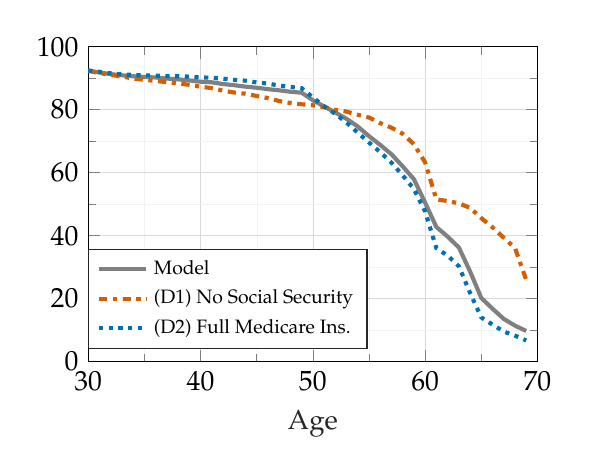
\begin{tikzpicture}
\begin{axis}[%
width=5.706cm,
height=4cm,
at={(0cm,0cm)},
scale only axis,
xmin=30,
xmax=70,
xlabel style={font=\color{white!15!black}},
xlabel={Age},
ymin=-0,
ymax=0100,
ylabel style={font=\color{white!15!black}},
ylabel={},
axis background/.style={fill=white},
%title style={font=\bfseries},
title={},
legend style={at={(axis cs:30,20)}, anchor=west, legend cell align=left, align=left, draw=white!15!black, font=\scriptsize},
grid=both,
grid style={line width=0.2pt, draw=gray!30},
minor grid style={line width=0.1pt, draw=gray!10},
minor tick num=1
]
% Back line (Overall) - full
\addplot [color=gray, line width=1.5pt]
  table[row sep=crcr]{%
30		92.457143	\\
31		91.828571	\\
32		91.314286	\\
33		90.942857	\\
34		90.657143	\\
35		90.4	\\
36		90.257143	\\
37		89.914286	\\
38		89.657143	\\
39		89.314286	\\
40		88.914286	\\
41		88.714286	\\
42		88.171429	\\
43		87.8	\\
44		87.342857	\\
45		87	\\
46		86.542857	\\
47		86.171429	\\
48		85.714286	\\
49		85.428571	\\
50		83.028571	\\
51		81.057143	\\
52		79.142857	\\
53		77.114286	\\
54		74.685714	\\
55		71.628571	\\
56		68.857143	\\
57		65.885714	\\
58		62.028571	\\
59		57.971429	\\
60		50.485714	\\
61		42.771429	\\
62		39.714286	\\
63		36.285714	\\
64		28.657143	\\
65		20.228571	\\
66		16.828571	\\
67		13.6	\\
68		11.457143	\\
69		9.771429	\\
};
\addlegendentry{Model}
% Blue line (Good health) - dotted
\addplot [color=red, line width=1.5pt, dashdotted]
  table[row sep=crcr]{%
30	92.342857	\\
31	91.685714	\\
32	91.057143	\\
33	90.571429	\\
34	89.914286	\\
35	89.514286	\\
36	89.171429	\\
37	88.742857	\\
38	88.371429	\\
39	87.914286	\\
40	87.342857	\\
41	86.857143	\\
42	86.057143	\\
43	85.485714	\\
44	85.085714	\\
45	84.371429	\\
46	83.714286	\\
47	82.771429	\\
48	82.142857	\\
49	81.742857	\\
50	81.428571	\\
51	80.857143	\\
52	79.971429	\\
53	79.428571	\\
54	78.4	\\
55	77.542857	\\
56	75.742857	\\
57	74.314286	\\
58	72.4	\\
59	69.057143	\\
60	63.285714	\\
61	51.542857	\\
62	51.028571	\\
63	50.285714	\\
64	48.857143	\\
65	45.6	\\
66	42.657143	\\
67	39.342857	\\
68	36.114286	\\
69	25.971429	\\
};
\addlegendentry{(D1) No Social Security}

% Red line (Poor health) - dash-dotted
\addplot [color=blue, line width=1.5pt, dotted]
  table[row sep=crcr]{%
30	92.485714	\\
31	92.028571	\\
32	91.6	\\
33	91.228571	\\
34	91.057143	\\
35	90.942857	\\
36	90.857143	\\
37	90.685714	\\
38	90.628571	\\
39	90.514286	\\
40	90.285714	\\
41	90.142857	\\
42	89.885714	\\
43	89.485714	\\
44	89.228571	\\
45	88.685714	\\
46	88.314286	\\
47	87.685714	\\
48	87.257143	\\
49	86.857143	\\
50	83.942857	\\
51	81.085714	\\
52	78.714286	\\
53	75.914286	\\
54	72.742857	\\
55	69.6	\\
56	66.542857	\\
57	63.2	\\
58	59.171429	\\
59	54.857143	\\
60	47.685714	\\
61	36.057143	\\
62	33.714286	\\
63	30.314286	\\
64	21.857143	\\
65	14.057143	\\
66	11.8	\\
67	9.571429	\\
68	8.285714	\\
69	6.742857	\\
};
\addlegendentry{(D2) Full Medicare Ins.}

% Green line (Disabled) - dashed
% \addplot [color=green, line width=1.5pt, dashed]
%   table[row sep=crcr]{%
% 30	92.6	\\
% 31	92.2	\\
% 32	91.7714286	\\
% 33	91.4285714	\\
% 34	91.2571429	\\
% 35	91.1142857	\\
% 36	91.0571429	\\
% 37	90.8857143	\\
% 38	90.8285714	\\
% 39	90.7142857	\\
% 40	90.4571429	\\
% 41	90.2857143	\\
% 42	90.0285714	\\
% 43	89.6571429	\\
% 44	89.3142857	\\
% 45	88.7714286	\\
% 46	88.2857143	\\
% 47	87.6571429	\\
% 48	87.1714286	\\
% 49	86.6285714	\\
% 50	83.7142857	\\
% 51	80.8285714	\\
% 52	78.5428571	\\
% 53	75.9142857	\\
% 54	72.8857143	\\
% 55	69.7428571	\\
% 56	66.6285714	\\
% 57	63.1428571	\\
% 58	59.0857143	\\
% 59	54.7714286	\\
% 60	47.2571429	\\
% 61	35.0571429	\\
% 62	32.8285714	\\
% 63	29.5714286	\\
% 64	21.0571429	\\
% 65	5.5714286	\\
% 66	3.1428571	\\
% 67	2.0285714	\\
% 68	1.3428571	\\
% 69	0.7142857	\\
% };
% \addlegendentry{Medicare B Reform Full}
\end{axis}
\end{tikzpicture} & 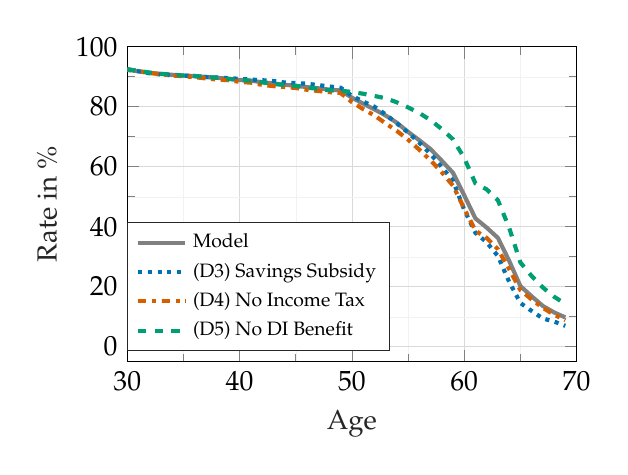
\begin{tikzpicture}
\begin{axis}[%
width=5.706cm,
height=4cm,
at={(0cm,0cm)},
scale only axis,
xmin=30,
xmax=70,
xlabel style={font=\color{white!15!black}},
xlabel={Age},
ymin=-5,
ytick={0,20,...,100},
ymax=0100,
ylabel style={font=\color{white!15!black}},
ylabel={Rate in \%},
axis background/.style={fill=white},
%title style={font=\bfseries},
title={},
legend style={at={(axis cs:30,20)}, anchor=west, legend cell align=left, align=left, draw=white!15!black, font=\scriptsize},
grid=both,
grid style={line width=0.2pt, draw=gray!30},
minor grid style={line width=0.1pt, draw=gray!10},
minor tick num=1
]
% Back line (Overall) - full
\addplot [color=gray, line width=1.5pt]
  table[row sep=crcr]{%
30		92.457143	\\
31		91.828571	\\
32		91.314286	\\
33		90.942857	\\
34		90.657143	\\
35		90.4	\\
36		90.257143	\\
37		89.914286	\\
38		89.657143	\\
39		89.314286	\\
40		88.914286	\\
41		88.714286	\\
42		88.171429	\\
43		87.8	\\
44		87.342857	\\
45		87	\\
46		86.542857	\\
47		86.171429	\\
48		85.714286	\\
49		85.428571	\\
50		83.028571	\\
51		81.057143	\\
52		79.142857	\\
53		77.114286	\\
54		74.685714	\\
55		71.628571	\\
56		68.857143	\\
57		65.885714	\\
58		62.028571	\\
59		57.971429	\\
60		50.485714	\\
61		42.771429	\\
62		39.714286	\\
63		36.285714	\\
64		28.657143	\\
65		20.228571	\\
66		16.828571	\\
67		13.6	\\
68		11.457143	\\
69		9.771429	\\
};
\addlegendentry{Model}


% Red line (Poor health) - dash-dotted
\addplot [color=blue, line width=1.5pt, dotted]
  table[row sep=crcr]{%
30	92.285714	\\
31	91.828571	\\
32	91.142857	\\
33	90.742857	\\
34	90.542857	\\
35	90.4	\\
36	90.2	\\
37	89.914286	\\
38	89.742857	\\
39	89.542857	\\
40	89.314286	\\
41	89.057143	\\
42	88.857143	\\
43	88.6	\\
44	88.085714	\\
45	87.914286	\\
46	87.685714	\\
47	87.228571	\\
48	86.771429	\\
49	86.342857	\\
50	83.657143	\\
51	81.742857	\\
52	80.028571	\\
53	77.457143	\\
54	74.485714	\\
55	71.4	\\
56	68	\\
57	64.228571	\\
58	59.942857	\\
59	55.285714	\\
60	45.657143	\\
61	37.971429	\\
62	34.828571	\\
63	30.228571	\\
64	21.657143	\\
65	14.6	\\
66	11.942857	\\
67	9.428571	\\
68	8.4	\\
69	6.971429	\\
};
\addlegendentry{(D3) Savings Subsidy}
% Blue line (Good health) - dotted
\addplot [color=red, line width=1.5pt, dashdotted]
  table[row sep=crcr]{%
30	92.485714	\\
31	91.857143	\\
32	91.257143	\\
33	90.857143	\\
34	90.428571	\\
35	90.171429	\\
36	89.857143	\\
37	89.457143	\\
38	89.085714	\\
39	88.857143	\\
40	88.314286	\\
41	88.028571	\\
42	87.314286	\\
43	86.885714	\\
44	86.6	\\
45	86.257143	\\
46	85.657143	\\
47	85.257143	\\
48	84.885714	\\
49	84.571429	\\
50	81.571429	\\
51	79.228571	\\
52	77.114286	\\
53	74.485714	\\
54	71.942857	\\
55	69.028571	\\
56	65.685714	\\
57	62.171429	\\
58	58.171429	\\
59	53.714286	\\
60	46.114286	\\
61	38.685714	\\
62	36.257143	\\
63	32.514286	\\
64	25.885714	\\
65	18.914286	\\
66	15.771429	\\
67	12.971429	\\
68	10.685714	\\
69	8.857143	\\
};
\addlegendentry{(D4) No Income Tax}


% Green line (Disabled) - dashed
\addplot [color=green, line width=1.5pt, dashed]
  table[row sep=crcr]{%
30	92.542857	\\
31	91.914286	\\
32	91.4	\\
33	90.971429	\\
34	90.742857	\\
35	90.4	\\
36	90.257143	\\
37	89.942857	\\
38	89.657143	\\
39	89.314286	\\
40	88.942857	\\
41	88.685714	\\
42	88.171429	\\
43	87.6	\\
44	87.257143	\\
45	86.942857	\\
46	86.371429	\\
47	85.971429	\\
48	85.485714	\\
49	85.342857	\\
50	84.942857	\\
51	84.342857	\\
52	83.6	\\
53	82.857143	\\
54	81.485714	\\
55	79.8	\\
56	77.914286	\\
57	75.542857	\\
58	72.571429	\\
59	69.142857	\\
60	62.942857	\\
61	54.428571	\\
62	52.457143	\\
63	48.828571	\\
64	39.685714	\\
65	28.114286	\\
66	23.6	\\
67	19.742857	\\
68	16.685714	\\
69	14.285714	\\
};
\addlegendentry{(D5) No DI Benefit}
\end{axis}
\end{tikzpicture}
\end{tabular}
\tabnotes{\textit{Notes:} Labor force participation rate (percent) by age, simulated from the estimated model (Model) and from counterfactual economies that eliminate one policy instrument. Left panel: the \textit{No Social Security} experiment (D1) sets Social Security benefits to zero; the \textit{Full Medicare Insurance} experiment (D2) sets out-of-pocket medical expenses after age 65 to zero for participants and nonparticipants. Right panel: the \textit{Full Savings Subsidy} experiment (D3) sets the net return on assets equal to the pretax return; the \textit{No Income Tax} experiment (D4) sets the income tax to zero; the \textit{No Disability Benefit} experiment (D5) sets disability benefits to zero. The \textit{No Social Security} experiment produces the largest increase in participation, followed by the \textit{No Disability Benefit} experiment. Welfare effects are in \autoref{tab:elim}.}
\end{figure}

\paragraph{Upper replacement rates.} \autoref{tab:generosity_app} reports reforms that raise the second replacement rate of the PIA formula from 0.32 to 0.352 (P2.0--P2.9) and then the third from 0.15 to 0.165 (P3.0--P3.9), in steps of 1 percent of the initial rate. All of them keep the first rate at 0.99, the value under P1.9, so each row, MVPF included, reports the total effect relative to the status quo, and the effect of the upper rates is the difference between a row and P1.9 in \autoref{tab:generosity}. Across P2.0--P2.9, the cumulative MVPF falls from 0.56 to 0.29: WTP rises from 0.83 to 0.95 percent, while the net cost more than doubles, from 0.57 to 1.27 percent. Relative to P1.9, P2.9 adds 0.15 percent to WTP and 0.83 percent to the net cost. Raising the third rate changes neither WTP nor the net cost by more than a few hundredths of a percentage point, within the precision of the simulations, and the MVPF stays at 0.29--0.30. Participation at 30--49 rises by 0.24 to 0.28 points, and participation at 62--64 and 65--69 falls by 0.83 to 2.41 points, more than under any bottom-bracket reform. P3.9 and L9 set the same three rates, (0.99, 0.352, 0.165), and their rows coincide.

\begin{table}[!htbp]
\centering
\caption{Reforms of the Upper Replacement Rates}\label{tab:generosity_app}
\footnotesize
\setlength{\tabcolsep}{4.5pt}
% Source: FROT tables/welfare_progressivity_mvpfv7.tex, rows P2 and P3.
% AUTHORS: reform and elimination results are from the May 2025 simulation; fit figures are the 2026 corrected re-simulation. Rerun reforms on the corrected code before submission.
% Generated by gen_tables.py from FROT tables/welfare_progressivity_mvpfv7.tex (rows P2, P3).
% Source numbers: May 2025 simulation of the estimated model (FROT 2025 submission). Do not edit numbers by hand.
\begin{tabular}{@{}l l c c c c c c c c@{}}
\toprule
 & & \multicolumn{2}{c}{Welfare} & \multicolumn{3}{c}{Fiscal cost (\% change)} & \multicolumn{3}{c}{$\Delta$ Participation (pp)} \\
\cmidrule(lr){3-4}\cmidrule(lr){5-7}\cmidrule(lr){8-10}
 & PIA rates & MVPF & WTP (\%) & Net & Direct & Indirect & 30--49 & 62--64 & 65--69 \\
\midrule
\multicolumn{10}{@{}l}{\textit{A. Raising the second PIA rate (first rate at 0.99)}} \\
(P2.0) & (0.99, 0.3232, 0.15) & 0.56 & 0.83 & 0.57 & 4.75 & $-$0.07 & 0.25 & $-$1.10 & $-$0.83 \\
(P2.1) & (0.99, 0.3264, 0.15) & 0.50 & 0.86 & 0.67 & 5.28 & $-$0.05 & 0.24 & $-$1.29 & $-$1.03 \\
(P2.2) & (0.99, 0.3296, 0.15) & 0.49 & 0.88 & 0.70 & 5.99 & $-$0.11 & 0.25 & $-$1.05 & $-$1.01 \\
(P2.3) & (0.99, 0.3328, 0.15) & 0.44 & 0.90 & 0.78 & 6.56 & $-$0.10 & 0.24 & $-$1.37 & $-$1.15 \\
(P2.4) & (0.99, 0.336, 0.15) & 0.38 & 0.92 & 0.93 & 7.21 & $-$0.05 & 0.24 & $-$1.60 & $-$1.63 \\
(P2.5) & (0.99, 0.3392, 0.15) & 0.37 & 0.93 & 0.98 & 7.95 & $-$0.10 & 0.27 & $-$1.63 & $-$1.58 \\
(P2.6) & (0.99, 0.3424, 0.15) & 0.36 & 0.95 & 1.03 & 8.46 & $-$0.11 & 0.28 & $-$1.47 & $-$1.68 \\
(P2.7) & (0.99, 0.3456, 0.15) & 0.33 & 0.94 & 1.11 & 8.99 & $-$0.10 & 0.27 & $-$1.74 & $-$1.99 \\
(P2.8) & (0.99, 0.3488, 0.15) & 0.31 & 0.95 & 1.19 & 9.49 & $-$0.10 & 0.28 & $-$2.29 & $-$2.10 \\
(P2.9) & (0.99, 0.352, 0.15) & 0.29 & 0.95 & 1.27 & 9.97 & $-$0.09 & 0.28 & $-$2.26 & $-$2.05 \\
\addlinespace
\multicolumn{10}{@{}l}{\textit{B. Raising the third PIA rate (first two rates at 0.99 and 0.352)}} \\
(P3.0) & (0.99, 0.352, 0.1515) & 0.29 & 0.95 & 1.26 & 10.04 & $-$0.10 & 0.28 & $-$2.22 & $-$2.05 \\
(P3.1) & (0.99, 0.352, 0.153) & 0.29 & 0.96 & 1.27 & 10.13 & $-$0.10 & 0.28 & $-$2.30 & $-$2.07 \\
(P3.2) & (0.99, 0.352, 0.1545) & 0.29 & 0.96 & 1.28 & 10.19 & $-$0.10 & 0.28 & $-$2.30 & $-$2.07 \\
(P3.3) & (0.99, 0.352, 0.156) & 0.29 & 0.96 & 1.26 & 10.26 & $-$0.13 & 0.28 & $-$2.25 & $-$2.03 \\
(P3.4) & (0.99, 0.352, 0.1575) & 0.29 & 0.96 & 1.27 & 10.34 & $-$0.13 & 0.28 & $-$2.23 & $-$2.03 \\
(P3.5) & (0.99, 0.352, 0.159) & 0.29 & 0.97 & 1.29 & 10.41 & $-$0.12 & 0.28 & $-$2.41 & $-$2.02 \\
(P3.6) & (0.99, 0.352, 0.1605) & 0.29 & 0.97 & 1.27 & 10.48 & $-$0.14 & 0.28 & $-$2.39 & $-$2.02 \\
(P3.7) & (0.99, 0.352, 0.162) & 0.30 & 0.97 & 1.27 & 10.55 & $-$0.15 & 0.28 & $-$2.39 & $-$2.02 \\
(P3.8) & (0.99, 0.352, 0.1635) & 0.30 & 0.97 & 1.25 & 10.63 & $-$0.18 & 0.28 & $-$2.37 & $-$2.01 \\
(P3.9) & (0.99, 0.352, 0.165) & 0.30 & 0.98 & 1.24 & 10.70 & $-$0.20 & 0.28 & $-$2.37 & $-$1.99 \\
\bottomrule
\end{tabular}

\tabnotes{\textit{Notes:} Each row reports the outcomes of simulating the estimated model for the cohort under the reform, announced before age 30 and in force over the life cycle, with prices held fixed (partial equilibrium). The second column gives the three replacement rates of the PIA formula; the status quo is (0.90, 0.32, 0.15). P2.0--P2.9 raise the second rate in steps of 0.32 percentage points with the first rate at 0.99; P3.0--P3.9 raise the third rate in steps of 0.15 percentage points with the first two rates at 0.99 and 0.352. Every row includes the increase of the first rate to 0.99 (P1.9 in \autoref{tab:generosity}) and reports the change from the status quo. WTP: ex ante consumption-equivalent welfare change at age 30, in percent. Direct: percentage change in the present value of Social Security retirement benefits. Indirect: percentage change in the present value of all other taxes and transfers (DI benefits and consumption-floor transfers, net of income- and payroll-tax revenue). Net: percentage change in the present value of net government spending. Present values are per capita and discounted to age 62 (Section~\ref{sec:fw_fiscal}); because the three fiscal columns have different bases, Net is not the sum of Direct and Indirect. MVPF: WTP valued with the present value of per capita baseline consumption from age 62, divided by the dollar change in net government spending (equation~\eqref{eq:mvpf}). $\Delta$ Participation: change in the labor force participation rate at the indicated ages, in percentage points. Abbreviations: AIME, average indexed monthly earnings; DI, disability insurance; PIA, primary insurance amount.}
\end{table}

\begin{figure}[!htbp]
\centering
\caption{Participation under the Elimination of Policy Instruments, by Health Status}\label{fig:elim_lfpr_health}
\vspace{0.5em}
% Panels copied verbatim from the FROT project (figures/abdou/frot_weld{1,2}_{0,1,2}.tex), arranged as in FROT 2025_sub/12_app_quant.tex; scaled to 0.9 to fit the page.
% AUTHORS: reform and elimination results are from the May 2025 simulation; fit figures are the 2026 corrected re-simulation. Rerun reforms on the corrected code before submission.
\begin{tabular}{@{}c@{\hspace{1em}}c@{}}
\multicolumn{2}{c}{\small (A) Good Health}\\[0.3ex]
\scalebox{0.9}{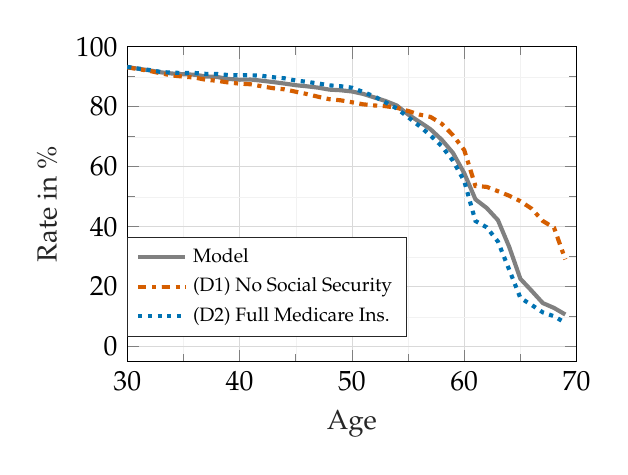
\begin{tikzpicture}
\begin{axis}[%
width=5.706cm,
height=4cm,
at={(0cm,0cm)},
scale only axis,
xmin=30,
xmax=70,
xlabel style={font=\color{white!15!black}},
xlabel={Age},
ymin=-5,
ytick={0,20,...,100},
ymax=0100,
ylabel style={font=\color{white!15!black}},
ylabel={Rate in \%},
axis background/.style={fill=white},
%title style={font=\bfseries},
title={},
legend style={at={(axis cs:30,20)}, anchor=west, legend cell align=left, align=left, draw=white!15!black, font=\scriptsize},
grid=both,
grid style={line width=0.2pt, draw=gray!30},
minor grid style={line width=0.1pt, draw=gray!10},
minor tick num=1
]
% Back line (Overall) - full
\addplot [color=gray, line width=1.5pt]
  table[row sep=crcr]{%
30	93.248945	\\
31	92.66386	\\
32	92.127404	\\
33	91.477788	\\
34	91.08492	\\
35	90.842714	\\
36	90.681332	\\
37	90.107527	\\
38	89.928947	\\
39	89.275723	\\
40	89.028213	\\
41	89.071383	\\
42	88.68104	\\
43	88.224061	\\
44	87.736151	\\
45	87.191157	\\
46	86.816406	\\
47	86.369637	\\
48	85.709527	\\
49	85.508219	\\
50	85.099111	\\
51	84.293015	\\
52	83.102493	\\
53	81.913775	\\
54	80.404686	\\
55	77.450628	\\
56	75	\\
57	72.50185	\\
58	68.992537	\\
59	64.610144	\\
60	57.880539	\\
61	49.142634	\\
62	46.258503	\\
63	42.21861	\\
64	33.333333	\\
65	22.642293	\\
66	18.667798	\\
67	14.554196	\\
68	12.927257	\\
69	10.749331	\\
};
\addlegendentry{Model}
% Blue line (Good health) - dotted
\addplot [color=red, line width=1.5pt, dashdotted]
  table[row sep=crcr]{%
30	93.128391	\\
31	92.543596	\\
32	91.947115	\\
33	91.145361	\\
34	90.420066	\\
35	90.051719	\\
36	89.734189	\\
37	89.001536	\\
38	88.662342	\\
39	88.094498	\\
40	87.711599	\\
41	87.492104	\\
42	86.810399	\\
43	86.187142	\\
44	85.814922	\\
45	85.013004	\\
46	84.244792	\\
47	83.333333	\\
48	82.511659	\\
49	82.15364	\\
50	81.510595	\\
51	80.817717	\\
52	80.436288	\\
53	80.196285	\\
54	79.659212	\\
55	78.599641	\\
56	77.405248	\\
57	76.609919	\\
58	74.328358	\\
59	70.514762	\\
60	65.587669	\\
61	53.585347	\\
62	53.301321	\\
63	51.848842	\\
64	50.347648	\\
65	48.525135	\\
66	46.033093	\\
67	41.914336	\\
68	39.658195	\\
69	29.125781	\\
};
\addlegendentry{(D1) No Social Security}

% Red line (Poor health) - dash-dotted
\addplot [color=blue, line width=1.5pt, dotted]
  table[row sep=crcr]{%
30	93.279084	\\
31	92.723993	\\
32	92.247596	\\
33	91.59867	\\
34	91.356905	\\
35	91.268634	\\
36	91.261839	\\
37	90.967742	\\
38	90.917516	\\
39	90.581287	\\
40	90.470219	\\
41	90.524321	\\
42	90.298034	\\
43	89.847231	\\
44	89.497278	\\
45	88.751625	\\
46	88.313802	\\
47	87.755776	\\
48	87.141905	\\
49	86.85005	\\
50	86.363636	\\
51	84.940375	\\
52	83.448753	\\
53	81.458114	\\
54	79.410721	\\
55	76.552962	\\
56	73.61516	\\
57	70.429312	\\
58	66.865672	\\
59	61.998486	\\
60	55.260116	\\
61	41.93297	\\
62	39.815926	\\
63	35.067046	\\
64	25.725971	\\
65	16.285833	\\
66	13.915995	\\
67	11.451049	\\
68	10.166521	\\
69	7.983943	\\
};
\addlegendentry{(D2) Full Medicare Ins.}

% % Green line (Disabled) - dashed
% \addplot [color=green, line width=1.5pt, dashed]
%   table[row sep=crcr]{%
% 30	88.42857143	\\
% 31	88.22857143	\\
% 32	87.85714286	\\
% 33	86.77142857	\\
% 34	86.57142857	\\
% 35	85.88571429	\\
% 36	85.51428571	\\
% 37	84.77142857	\\
% 38	84.25714286	\\
% 39	83.45714286	\\
% 40	82.62857143	\\
% 41	82.02857143	\\
% 42	81.51428571	\\
% 43	80.82857143	\\
% 44	79.97142857	\\
% 45	78.08571429	\\
% 46	77.54285714	\\
% 47	76	\\
% 48	74.71428571	\\
% 49	73.77142857	\\
% 50	72.02857143	\\
% 51	70.97142857	\\
% 52	68.62857143	\\
% 53	66.31428571	\\
% 54	63.85714286	\\
% 55	60.91428571	\\
% 56	57.57142857	\\
% 57	54.2	\\
% 58	51.11428571	\\
% 59	46.62857143	\\
% 60	40.71428571	\\
% 61	29.94285714	\\
% 62	27.68571429	\\
% 63	23.88571429	\\
% 64	17.48571429	\\
% 65	5.314285714	\\
% 66	3	\\
% 67	1.942857143	\\
% 68	1.257142857	\\
% 69	0.685714286	\\
% };
% \addlegendentry{Medicare B Reform Full}
\end{axis}
\end{tikzpicture}} & \scalebox{0.9}{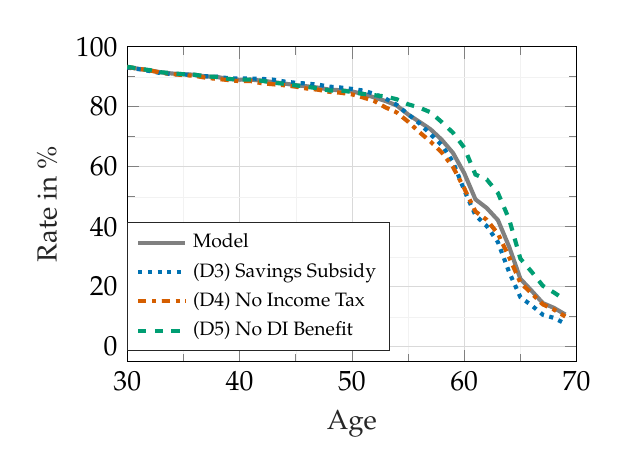
\begin{tikzpicture}
\begin{axis}[%
width=5.706cm,
height=4cm,
at={(0cm,0cm)},
scale only axis,
xmin=30,
xmax=70,
xlabel style={font=\color{white!15!black}},
xlabel={Age},
ymin=-5,
ytick={0,20,...,100},
ymax=0100,
ylabel style={font=\color{white!15!black}},
ylabel={Rate in \%},
axis background/.style={fill=white},
%title style={font=\bfseries},
title={},
legend style={at={(axis cs:30,20)}, anchor=west, legend cell align=left, align=left, draw=white!15!black, font=\scriptsize},
grid=both,
grid style={line width=0.2pt, draw=gray!30},
minor grid style={line width=0.1pt, draw=gray!10},
minor tick num=1
]
% Back line (Overall) - full
\addplot [color=gray, line width=1.5pt]
  table[row sep=crcr]{%
30	93.248945	\\
31	92.66386	\\
32	92.127404	\\
33	91.477788	\\
34	91.08492	\\
35	90.842714	\\
36	90.681332	\\
37	90.107527	\\
38	89.928947	\\
39	89.275723	\\
40	89.028213	\\
41	89.071383	\\
42	88.68104	\\
43	88.224061	\\
44	87.736151	\\
45	87.191157	\\
46	86.816406	\\
47	86.369637	\\
48	85.709527	\\
49	85.508219	\\
50	85.099111	\\
51	84.293015	\\
52	83.102493	\\
53	81.913775	\\
54	80.404686	\\
55	77.450628	\\
56	75	\\
57	72.50185	\\
58	68.992537	\\
59	64.610144	\\
60	57.880539	\\
61	49.142634	\\
62	46.258503	\\
63	42.21861	\\
64	33.333333	\\
65	22.642293	\\
66	18.667798	\\
67	14.554196	\\
68	12.927257	\\
69	10.749331	\\
};
\addlegendentry{Model}


% Red line (Poor health) - dash-dotted
\addplot [color=blue, line width=1.5pt, dotted]
  table[row sep=crcr]{%
30	93.068113	\\
31	92.543596	\\
32	91.917067	\\
33	91.205802	\\
34	90.903596	\\
35	90.751445	\\
36	90.55912	\\
37	90.168971	\\
38	90.021625	\\
39	89.524402	\\
40	89.404389	\\
41	89.418825	\\
42	89.28345	\\
43	89.05156	\\
44	88.408581	\\
45	88.003901	\\
46	87.727865	\\
47	87.359736	\\
48	86.708861	\\
49	86.413955	\\
50	85.95352	\\
51	85.417376	\\
52	84.279778	\\
53	82.719944	\\
54	80.617678	\\
55	77.522442	\\
56	74.489796	\\
57	70.873427	\\
58	67.201493	\\
59	61.619985	\\
60	52.2158	\\
61	43.842557	\\
62	40.256102	\\
63	34.863876	\\
64	24.867076	\\
65	16.535106	\\
66	13.788714	\\
67	10.664336	\\
68	9.596845	\\
69	7.671722	\\
};
\addlegendentry{(D3) Savings Subsidy}


% Blue line (Good health) - dotted
\addplot [color=red, line width=1.5pt, dashdotted]
  table[row sep=crcr]{%
30	93.279084	\\
31	92.66386	\\
32	92.097356	\\
33	91.387126	\\
34	90.873376	\\
35	90.568908	\\
36	90.314696	\\
37	89.677419	\\
38	89.280198	\\
39	88.902704	\\
40	88.526646	\\
41	88.566014	\\
42	87.824984	\\
43	87.492043	\\
44	87.159782	\\
45	86.703511	\\
46	86.067708	\\
47	85.676568	\\
48	84.976682	\\
49	84.669574	\\
50	84.142174	\\
51	83.100511	\\
52	81.890582	\\
53	79.775675	\\
54	78.097267	\\
55	75.044883	\\
56	71.574344	\\
57	68.393782	\\
58	64.776119	\\
59	59.91673	\\
60	52.83237	\\
61	45.089634	\\
62	42.336935	\\
63	37.667615	\\
64	29.856851	\\
65	21.354383	\\
66	17.776835	\\
67	14.117133	\\
68	12.357581	\\
69	10.080285	\\
};
\addlegendentry{(D4) No Income Tax}
% Green line (Disabled) - dashed
\addplot [color=green, line width=1.5pt, dashed]
  table[row sep=crcr]{%
30	93.339361	\\
31	92.723993	\\
32	92.217548	\\
33	91.508008	\\
34	91.175582	\\
35	90.842714	\\
36	90.681332	\\
37	90.138249	\\
38	89.928947	\\
39	89.275723	\\
40	89.059561	\\
41	89.039798	\\
42	88.649334	\\
43	88.0331	\\
44	87.64009	\\
45	87.126138	\\
46	86.653646	\\
47	86.138614	\\
48	85.443038	\\
49	85.441127	\\
50	84.92823	\\
51	84.258944	\\
52	83.864266	\\
53	83.42096	\\
54	82.499113	\\
55	80.825853	\\
56	79.737609	\\
57	78.164323	\\
58	74.88806	\\
59	71.347464	\\
60	66.396917	\\
61	57.404521	\\
62	55.782313	\\
63	51.279967	\\
64	42.494888	\\
65	29.372663	\\
66	24.989393	\\
67	20.323427	\\
68	18.054338	\\
69	15.566459	\\
};
\addlegendentry{(D5) No DI Benefit}
\end{axis}
\end{tikzpicture}} \\[0.4ex]
\multicolumn{2}{c}{\small (B) Poor Health}\\[0.3ex]
\scalebox{0.9}{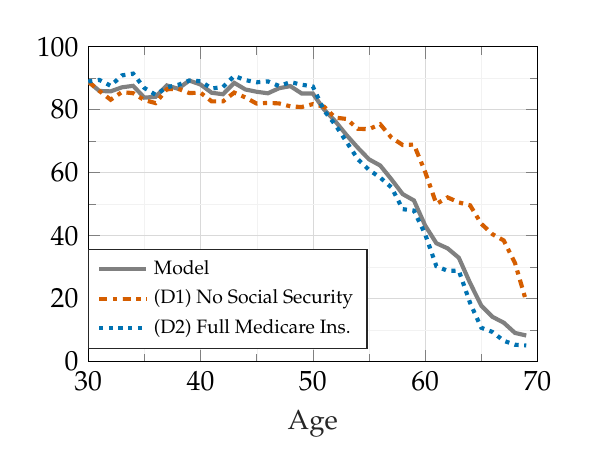
\begin{tikzpicture}
\begin{axis}[%
width=5.706cm,
height=4cm,
at={(0cm,0cm)},
scale only axis,
xmin=30,
xmax=70,
xlabel style={font=\color{white!15!black}},
xlabel={Age},
ymin=-0,
ymax=0100,
ylabel style={font=\color{white!15!black}},
ylabel={},
axis background/.style={fill=white},
%title style={font=\bfseries},
title={},
legend style={at={(axis cs:30,20)}, anchor=west, legend cell align=left, align=left, draw=white!15!black, font=\scriptsize},
grid=both,
grid style={line width=0.2pt, draw=gray!30},
minor grid style={line width=0.1pt, draw=gray!10},
minor tick num=1
]
% Back line (Overall) - full
\addplot [color=gray, line width=1.5pt]
  table[row sep=crcr]{%
30	88.970588	\\
31	85.964912	\\
32	85.840708	\\
33	87.121212	\\
34	87.596899	\\
35	83.846154	\\
36	84.10596	\\
37	87.730061	\\
38	86.666667	\\
39	89.265537	\\
40	88.020833	\\
41	85.388128	\\
42	84.931507	\\
43	88.546256	\\
44	86.440678	\\
45	85.714286	\\
46	85.227273	\\
47	86.851211	\\
48	87.5	\\
49	85.185185	\\
50	85.154062	\\
51	80.060423	\\
52	76.353276	\\
53	71.967655	\\
54	67.96875	\\
55	64.268585	\\
56	62.302483	\\
57	57.905983	\\
58	53.222453	\\
59	51.209677	\\
60	43.248532	\\
61	37.619962	\\
62	36	\\
63	33.004926	\\
64	25	\\
65	17.810458	\\
66	14.24	\\
67	12.389381	\\
68	9.145427	\\
69	8.333333	\\
};
\addlegendentry{Model}
% Blue line (Good health) - dotted
\addplot [color=red, line width=1.5pt, dashdotted]
  table[row sep=crcr]{%
30	88.970588	\\
31	85.964912	\\
32	83.185841	\\
33	85.606061	\\
34	85.271318	\\
35	83.076923	\\
36	82.119205	\\
37	86.503067	\\
38	86.666667	\\
39	85.310734	\\
40	85.416667	\\
41	82.648402	\\
42	82.648402	\\
43	85.462555	\\
44	83.898305	\\
45	81.954887	\\
46	82.19697	\\
47	82.00692	\\
48	81.089744	\\
49	80.864198	\\
50	81.792717	\\
51	80.966767	\\
52	77.492877	\\
53	77.088949	\\
54	73.958333	\\
55	73.860911	\\
56	75.395034	\\
57	71.153846	\\
58	68.814969	\\
59	68.951613	\\
60	60.273973	\\
61	50.095969	\\
62	52.173913	\\
63	50.574713	\\
64	49.666667	\\
65	43.79085	\\
66	40.48	\\
67	38.495575	\\
68	31.334333	\\
69	19.109195	\\
};
\addlegendentry{(D1) No Social Security}

% Red line (Poor health) - dash-dotted
\addplot [color=blue, line width=1.5pt, dotted]
  table[row sep=crcr]{%
30	88.970588	\\
31	89.473684	\\
32	87.610619	\\
33	90.909091	\\
34	91.472868	\\
35	86.923077	\\
36	84.768212	\\
37	87.116564	\\
38	87.878788	\\
39	89.265537	\\
40	89.0625	\\
41	86.757991	\\
42	87.214612	\\
43	90.748899	\\
44	89.40678	\\
45	88.721805	\\
46	89.015152	\\
47	87.543253	\\
48	88.782051	\\
49	87.962963	\\
50	87.394958	\\
51	79.758308	\\
52	75.213675	\\
53	69.811321	\\
54	64.322917	\\
55	60.911271	\\
56	58.465011	\\
57	55.34188	\\
58	48.440748	\\
59	47.983871	\\
60	40.508806	\\
61	30.326296	\\
62	28.869565	\\
63	28.899836	\\
64	18.666667	\\
65	10.784314	\\
66	9.44	\\
67	6.637168	\\
68	5.397301	\\
69	5.172414	\\
};
\addlegendentry{(D2) Full Medicare Ins.}

% % Green line (Disabled) - dashed
% \addplot [color=green, line width=1.5pt, dashed]
%   table[row sep=crcr]{%
% 30	91.91176471	\\
% 31	89.47368421	\\
% 32	88.49557522	\\
% 33	91.66666667	\\
% 34	91.47286822	\\
% 35	86.92307692	\\
% 36	85.43046358	\\
% 37	87.73006135	\\
% 38	88.48484848	\\
% 39	89.26553672	\\
% 40	89.0625	\\
% 41	86.75799087	\\
% 42	87.21461187	\\
% 43	90.74889868	\\
% 44	88.98305085	\\
% 45	88.72180451	\\
% 46	88.63636364	\\
% 47	87.5432526	\\
% 48	88.46153846	\\
% 49	87.34567901	\\
% 50	86.55462185	\\
% 51	79.15407855	\\
% 52	76.06837607	\\
% 53	70.08086253	\\
% 54	64.32291667	\\
% 55	60.19184652	\\
% 56	59.36794582	\\
% 57	55.55555556	\\
% 58	48.23284823	\\
% 59	47.58064516	\\
% 60	38.94324853	\\
% 61	28.59884837	\\
% 62	28	\\
% 63	28.40722496	\\
% 64	17.16666667	\\
% 65	0.653594771	\\
% 66	0.64	\\
% 67	0.147492625	\\
% 68	0.149925037	\\
% 69	0	\\
% };
% \addlegendentry{Medicare B Reform Full}
\end{axis}
\end{tikzpicture}} & \scalebox{0.9}{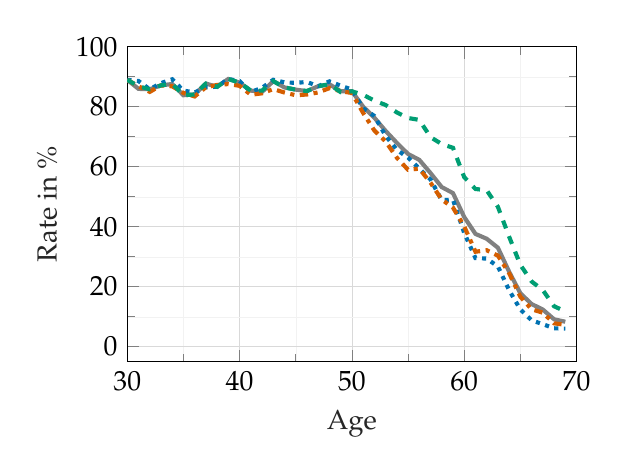
\begin{tikzpicture}
\begin{axis}[%
width=5.706cm,
height=4cm,
at={(0cm,0cm)},
scale only axis,
xmin=30,
xmax=70,
xlabel style={font=\color{white!15!black}},
xlabel={Age},
ymin=-5,
ytick={0,20,...,100},
ymax=0100,
ylabel style={font=\color{white!15!black}},
ylabel={Rate in \%},
axis background/.style={fill=white},
%title style={font=\bfseries},
title={},
legend style={at={(axis cs:30,20)}, anchor=west, legend cell align=left, align=left, draw=white!15!black, font=\scriptsize},
grid=both,
grid style={line width=0.2pt, draw=gray!30},
minor grid style={line width=0.1pt, draw=gray!10},
minor tick num=1
]
% Back line (Overall) - full
\addplot [color=gray, line width=1.5pt]
  table[row sep=crcr]{%
30	88.970588	\\
31	85.964912	\\
32	85.840708	\\
33	87.121212	\\
34	87.596899	\\
35	83.846154	\\
36	84.10596	\\
37	87.730061	\\
38	86.666667	\\
39	89.265537	\\
40	88.020833	\\
41	85.388128	\\
42	84.931507	\\
43	88.546256	\\
44	86.440678	\\
45	85.714286	\\
46	85.227273	\\
47	86.851211	\\
48	87.5	\\
49	85.185185	\\
50	85.154062	\\
51	80.060423	\\
52	76.353276	\\
53	71.967655	\\
54	67.96875	\\
55	64.268585	\\
56	62.302483	\\
57	57.905983	\\
58	53.222453	\\
59	51.209677	\\
60	43.248532	\\
61	37.619962	\\
62	36	\\
63	33.004926	\\
64	25	\\
65	17.810458	\\
66	14.24	\\
67	12.389381	\\
68	9.145427	\\
69	8.333333	\\
};
% \addlegendentry{Model} % legend shown in row (A) only

% Red line (Poor health) - dash-dotted
\addplot [color=blue, line width=1.5pt, dotted]
  table[row sep=crcr]{%
30	88.970588	\\
31	88.596491	\\
32	85.840708	\\
33	87.878788	\\
34	89.147287	\\
35	85.384615	\\
36	84.768212	\\
37	86.503067	\\
38	86.666667	\\
39	89.265537	\\
40	88.541667	\\
41	84.931507	\\
42	86.30137	\\
43	88.986784	\\
44	88.135593	\\
45	87.969925	\\
46	88.257576	\\
47	86.851211	\\
48	88.461538	\\
49	87.037037	\\
50	85.714286	\\
51	79.456193	\\
52	76.923077	\\
53	70.350404	\\
54	65.625	\\
55	63.069544	\\
56	59.367946	\\
57	55.769231	\\
58	48.856549	\\
59	48.991935	\\
60	37.964775	\\
61	29.558541	\\
62	29.391304	\\
63	26.765189	\\
64	18.833333	\\
65	12.418301	\\
66	8.8	\\
67	7.522124	\\
68	6.146927	\\
69	6.034483	\\
};
%\addlegendentry{(D3) No Cap. Gains Tax}
% \addlegendentry{(D3)} % legend shown in row (A) only
% Blue line (Good health) - dotted
\addplot [color=red, line width=1.5pt, dashdotted]
  table[row sep=crcr]{%
30	88.970588	\\
31	86.842105	\\
32	84.955752	\\
33	87.121212	\\
34	86.821705	\\
35	84.615385	\\
36	83.443709	\\
37	86.503067	\\
38	87.272727	\\
39	87.570621	\\
40	86.979167	\\
41	84.018265	\\
42	84.474886	\\
43	85.903084	\\
44	84.745763	\\
45	83.834586	\\
46	84.090909	\\
47	84.775087	\\
48	86.217949	\\
49	85.185185	\\
50	84.593838	\\
51	77.945619	\\
52	72.079772	\\
53	68.463612	\\
54	63.020833	\\
55	58.992806	\\
56	59.367946	\\
57	54.700855	\\
58	49.064449	\\
59	46.370968	\\
60	40.117417	\\
61	31.669866	\\
62	32.173913	\\
63	30.377668	\\
64	24.5	\\
65	16.666667	\\
66	12.48	\\
67	11.356932	\\
68	7.796102	\\
69	7.327586	\\
};
%\addlegendentry{(D4) No Income Tax}
% \addlegendentry{(D4)} % legend shown in row (A) only



% Green line (Disabled) - dashed
\addplot [color=green, line width=1.5pt, dashed]
  table[row sep=crcr]{%
30	88.970588	\\
31	86.842105	\\
32	85.840708	\\
33	87.121212	\\
34	87.596899	\\
35	83.846154	\\
36	84.10596	\\
37	87.730061	\\
38	86.666667	\\
39	89.265537	\\
40	88.020833	\\
41	85.388128	\\
42	85.388128	\\
43	88.546256	\\
44	86.440678	\\
45	85.714286	\\
46	85.227273	\\
47	86.851211	\\
48	87.5	\\
49	84.876543	\\
50	85.154062	\\
51	83.987915	\\
52	82.051282	\\
53	80.592992	\\
54	78.125	\\
55	76.258993	\\
56	75.620767	\\
57	69.871795	\\
58	67.567568	\\
59	66.330645	\\
60	56.555773	\\
61	52.591171	\\
62	52.173913	\\
63	46.633826	\\
64	36.666667	\\
65	27.287582	\\
66	21.76	\\
67	18.879056	\\
68	13.493253	\\
69	11.781609	\\
};
%\addlegendentry{(D5) No Disability Benefit}
% \addlegendentry{(D5)} % legend shown in row (A) only
\end{axis}
\end{tikzpicture}} \\[0.4ex]
\multicolumn{2}{c}{\small (C) Disability}\\[0.3ex]
\scalebox{0.9}{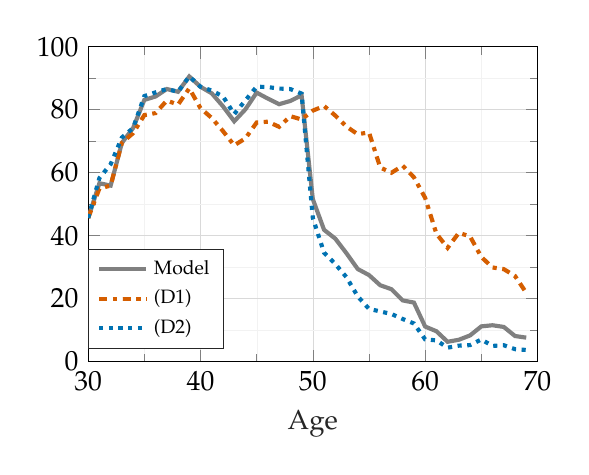
\begin{tikzpicture}
\begin{axis}[%
width=5.706cm,
height=4cm,
at={(0cm,0cm)},
scale only axis,
xmin=30,
xmax=70,
xlabel style={font=\color{white!15!black}},
xlabel={Age},
ymin=-0,
ymax=0100,
ylabel style={font=\color{white!15!black}},
ylabel={},
axis background/.style={fill=white},
%title style={font=\bfseries},
title={},
legend style={at={(axis cs:30,20)}, anchor=west, legend cell align=left, align=left, draw=white!15!black, font=\scriptsize},
grid=both,
grid style={line width=0.2pt, draw=gray!30},
minor grid style={line width=0.1pt, draw=gray!10},
minor tick num=1
]
% Back line (Overall) - full
\addplot [color=gray, line width=1.5pt]
  table[row sep=crcr]{%
30	45.652174	\\
31	56.666667	\\
32	55.932203	\\
33	69.491525	\\
34	74.193548	\\
35	83.13253	\\
36	84.210526	\\
37	86.585366	\\
38	85.714286	\\
39	90.566038	\\
40	87.288136	\\
41	85.217391	\\
42	81.102362	\\
43	76.335878	\\
44	80.141844	\\
45	85.443038	\\
46	83.536585	\\
47	81.767956	\\
48	82.795699	\\
49	84.615385	\\
50	51.612903	\\
51	41.880342	\\
52	39.08046	\\
53	34.42029	\\
54	29.431438	\\
55	27.516779	\\
56	24.28115	\\
57	23.030303	\\
58	19.469027	\\
59	18.78453	\\
60	11.167513	\\
61	9.68523	\\
62	6.338028	\\
63	6.976744	\\
64	8.351648	\\
65	11.226611	\\
66	11.583012	\\
67	11.048689	\\
68	8.166969	\\
69	7.651246	\\
};
\addlegendentry{Model}
% Blue line (Good health) - dotted
\addplot [color=red, line width=1.5pt, dashdotted]
  table[row sep=crcr]{%
30	45.652174	\\
31	55	\\
32	55.932203	\\
33	69.491525	\\
34	72.580645	\\
35	78.313253	\\
36	78.947368	\\
37	82.926829	\\
38	81.632653	\\
39	86.792453	\\
40	80.508475	\\
41	77.391304	\\
42	73.228346	\\
43	68.70229	\\
44	70.921986	\\
45	75.949367	\\
46	76.219512	\\
47	74.585635	\\
48	77.956989	\\
49	76.923077	\\
50	79.723502	\\
51	81.196581	\\
52	78.16092	\\
53	74.637681	\\
54	72.240803	\\
55	72.818792	\\
56	61.661342	\\
57	60	\\
58	62.241888	\\
59	58.563536	\\
60	52.030457	\\
61	40.677966	\\
62	36.150235	\\
63	40.930233	\\
64	39.78022	\\
65	33.264033	\\
66	29.92278	\\
67	29.400749	\\
68	27.22323	\\
69	21.886121	\\
};
%\addlegendentry{(D1) No Social Security}
\addlegendentry{(D1)}

% Red line (Poor health) - dash-dotted
\addplot [color=blue, line width=1.5pt, dotted]
  table[row sep=crcr]{%
30	45.652174	\\
31	58.333333	\\
32	62.711864	\\
33	71.186441	\\
34	74.193548	\\
35	84.337349	\\
36	85.526316	\\
37	86.585366	\\
38	85.714286	\\
39	90.566038	\\
40	87.288136	\\
41	86.086957	\\
42	84.251969	\\
43	78.625954	\\
44	82.978723	\\
45	87.341772	\\
46	87.195122	\\
47	86.740331	\\
48	86.55914	\\
49	85.128205	\\
50	45.62212	\\
51	34.615385	\\
52	31.034483	\\
53	26.811594	\\
54	20.735786	\\
55	16.778523	\\
56	15.974441	\\
57	15.151515	\\
58	13.569322	\\
59	12.154696	\\
60	7.106599	\\
61	6.779661	\\
62	4.460094	\\
63	5.116279	\\
64	5.274725	\\
65	7.068607	\\
66	5.019305	\\
67	5.243446	\\
68	3.99274	\\
69	3.736655	\\
};
%\addlegendentry{(D2) Full Medicare Ins.}
\addlegendentry{(D2)}

% Green line (Disabled) - dashed
% \addplot [color=green, line width=1.5pt, dashed]
%   table[row sep=crcr]{%
% 30	45.65217391	\\
% 31	61.66666667	\\
% 32	62.71186441	\\
% 33	71.18644068	\\
% 34	74.19354839	\\
% 35	84.3373494	\\
% 36	85.52631579	\\
% 37	86.58536585	\\
% 38	85.71428571	\\
% 39	90.56603774	\\
% 40	87.28813559	\\
% 41	86.08695652	\\
% 42	84.2519685	\\
% 43	78.6259542	\\
% 44	82.9787234	\\
% 45	87.34177215	\\
% 46	86.58536585	\\
% 47	85.63535912	\\
% 48	86.02150538	\\
% 49	85.64102564	\\
% 50	46.08294931	\\
% 51	35.47008547	\\
% 52	30.651341	\\
% 53	27.53623188	\\
% 54	23.07692308	\\
% 55	19.46308725	\\
% 56	17.25239617	\\
% 57	16.06060606	\\
% 58	13.86430678	\\
% 59	13.5359116	\\
% 60	7.614213198	\\
% 61	7.263922518	\\
% 62	4.460093897	\\
% 63	6.046511628	\\
% 64	4.835164835	\\
% 65	1.03950104	\\
% 66	0.193050193	\\
% 67	0.374531835	\\
% 68	0.362976407	\\
% 69	0.177935943	\\
% };
% \addlegendentry{Medicare B Reform Full}
\end{axis}
\end{tikzpicture}} & \scalebox{0.9}{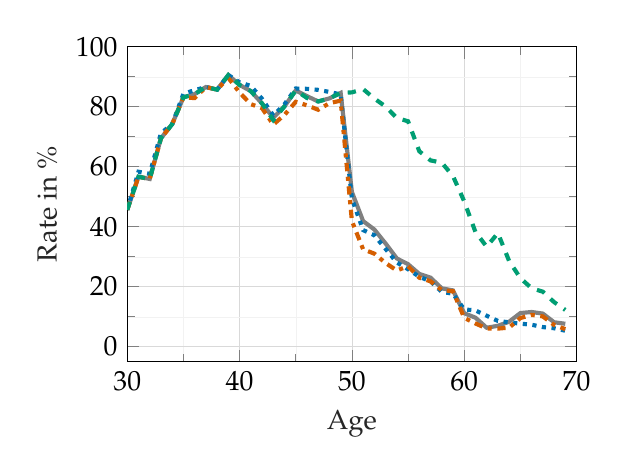
\begin{tikzpicture}
\begin{axis}[%
width=5.706cm,
height=4cm,
at={(0cm,0cm)},
scale only axis,
xmin=30,
xmax=70,
xlabel style={font=\color{white!15!black}},
xlabel={Age},
ymin=-5,
ytick={0,20,...,100},
ymax=0100,
ylabel style={font=\color{white!15!black}},
ylabel={Rate in \%},
axis background/.style={fill=white},
%title style={font=\bfseries},
title={},
legend style={at={(axis cs:30,20)}, anchor=west, legend cell align=left, align=left, draw=white!15!black, font=\scriptsize},
grid=both,
grid style={line width=0.2pt, draw=gray!30},
minor grid style={line width=0.1pt, draw=gray!10},
minor tick num=1
]
% Back line (Overall) - full
\addplot [color=gray, line width=1.5pt]
  table[row sep=crcr]{%
30	45.652174	\\
31	56.666667	\\
32	55.932203	\\
33	69.491525	\\
34	74.193548	\\
35	83.13253	\\
36	84.210526	\\
37	86.585366	\\
38	85.714286	\\
39	90.566038	\\
40	87.288136	\\
41	85.217391	\\
42	81.102362	\\
43	76.335878	\\
44	80.141844	\\
45	85.443038	\\
46	83.536585	\\
47	81.767956	\\
48	82.795699	\\
49	84.615385	\\
50	51.612903	\\
51	41.880342	\\
52	39.08046	\\
53	34.42029	\\
54	29.431438	\\
55	27.516779	\\
56	24.28115	\\
57	23.030303	\\
58	19.469027	\\
59	18.78453	\\
60	11.167513	\\
61	9.68523	\\
62	6.338028	\\
63	6.976744	\\
64	8.351648	\\
65	11.226611	\\
66	11.583012	\\
67	11.048689	\\
68	8.166969	\\
69	7.651246	\\
};
% \addlegendentry{Model} % legend shown in row (A) only

% Red line (Poor health) - dash-dotted
\addplot [color=blue, line width=1.5pt, dotted]
  table[row sep=crcr]{%
30	45.652174	\\
31	58.333333	\\
32	57.627119	\\
33	71.186441	\\
34	74.193548	\\
35	84.337349	\\
36	85.526316	\\
37	86.585366	\\
38	85.714286	\\
39	90.566038	\\
40	88.135593	\\
41	86.956522	\\
42	82.677165	\\
43	77.099237	\\
44	80.851064	\\
45	86.075949	\\
46	85.97561	\\
47	85.635359	\\
48	84.946237	\\
49	84.102564	\\
50	49.308756	\\
51	38.888889	\\
52	37.164751	\\
53	32.608696	\\
54	28.093645	\\
55	25.838926	\\
56	23.322684	\\
57	21.818182	\\
58	18.289086	\\
59	17.679558	\\
60	12.436548	\\
61	12.106538	\\
62	10.328638	\\
63	8.604651	\\
64	8.131868	\\
65	7.692308	\\
66	7.335907	\\
67	6.554307	\\
68	6.170599	\\
69	5.338078	\\
};
%\addlegendentry{(D3) No Cap. Gains Tax}
% \addlegendentry{(D3)} % legend shown in row (A) only
% Blue line (Good health) - dotted
\addplot [color=red, line width=1.5pt, dashdotted]
  table[row sep=crcr]{%
30	45.652174	\\
31	56.666667	\\
32	55.932203	\\
33	69.491525	\\
34	74.193548	\\
35	83.13253	\\
36	82.894737	\\
37	86.585366	\\
38	85.714286	\\
39	89.622642	\\
40	84.745763	\\
41	80.869565	\\
42	79.527559	\\
43	74.045802	\\
44	77.304965	\\
45	81.64557	\\
46	80.487805	\\
47	79.005525	\\
48	81.182796	\\
49	82.051282	\\
50	41.935484	\\
51	32.478632	\\
52	31.034483	\\
53	27.898551	\\
54	25.41806	\\
55	26.845638	\\
56	23.003195	\\
57	21.818182	\\
58	18.879056	\\
59	18.508287	\\
60	9.64467	\\
61	7.748184	\\
62	6.103286	\\
63	6.046512	\\
64	6.373626	\\
65	9.56341	\\
66	10.617761	\\
67	10.11236	\\
68	7.259528	\\
69	5.871886	\\
};
%\addlegendentry{(D4) No Income Tax}
% \addlegendentry{(D4)} % legend shown in row (A) only


% Green line (Disabled) - dashed
\addplot [color=green, line width=1.5pt, dashed]
  table[row sep=crcr]{%
30	45.652174	\\
31	56.666667	\\
32	55.932203	\\
33	69.491525	\\
34	74.193548	\\
35	83.13253	\\
36	84.210526	\\
37	86.585366	\\
38	85.714286	\\
39	90.566038	\\
40	87.288136	\\
41	85.217391	\\
42	81.102362	\\
43	75.572519	\\
44	80.141844	\\
45	85.443038	\\
46	82.926829	\\
47	81.767956	\\
48	82.795699	\\
49	84.615385	\\
50	84.792627	\\
51	85.897436	\\
52	82.758621	\\
53	80.072464	\\
54	76.254181	\\
55	75.167785	\\
56	65.175719	\\
57	62.121212	\\
58	61.356932	\\
59	56.906077	\\
60	48.477157	\\
61	38.256659	\\
62	33.333333	\\
63	37.906977	\\
64	28.571429	\\
65	22.869023	\\
66	19.498069	\\
67	18.35206	\\
68	14.882033	\\
69	12.27758	\\
};
%\addlegendentry{(D5) No Disability Benefit}
% \addlegendentry{(D5)} % legend shown in row (A) only
\end{axis}
\end{tikzpicture}}
\end{tabular}
\tabnotes{\textit{Notes:} Labor force participation rate (percent) by age and health status, simulated from the estimated model (Model) and from counterfactual economies that eliminate one policy instrument. Rows (A), (B), and (C) show individuals in good health, in poor health, and with a disability. Left panels: D1 sets Social Security benefits to zero; D2 sets out-of-pocket medical expenses after age 65 to zero for participants and nonparticipants. Right panels: D3 sets the net return on assets equal to the pretax return; D4 sets the income tax to zero; D5 sets disability benefits to zero. Line styles are the same in every row; the legends of row (A) identify them.}
\end{figure}


\end{document}
